\documentclass[a4paper,11pt,oneside,titlepage,openright]{book}
\usepackage[italian]{babel}
\usepackage[utf8]{inputenc}
\usepackage{indentfirst}
\usepackage[dvips]{graphicx}
\usepackage{amssymb}
\usepackage{amsmath}
\usepackage{latexsym}
\usepackage{amsthm}
\usepackage{amsfonts}
\usepackage{lettrine}
\usepackage{epsfig}
\usepackage{hyperref}
\usepackage{graphicx}
\usepackage{color}
\usepackage{courier}
\usepackage[font={small,it}]{caption}
\usepackage{mdwlist}
\usepackage{listings}
\usepackage[T1]{fontenc}
\usepackage{booktabs}
\usepackage{longtable}
\usepackage{pdflscape}
\usepackage{rotating}
\usepackage[babel]{csquotes}
\usepackage{epigraph}
\usepackage{tabularx}
\usepackage[style=numeric-comp,useprefix,hyperref,backend=bibtex]{biblatex}
\usepackage{algorithm2e}

\bibliography{tex_files/bibliography/bibliography}

\pagestyle{headings}

\lstdefinelanguage{JavaScript}{
  morekeywords={typeof, new, true, false, catch, function, return, null, catch, switch, var, if, in, while, do, else, case, break},
  morecomment=[s]{/*}{*/},
  morecomment=[l]//,
  morestring=[b]",
  morestring=[b]'
}

\lstset{%
    % Basic design
    backgroundcolor=\color{background},
    basicstyle={\scriptsize\ttfamily},
    frame=none,
    % Line numbers
    numbers=none,
    % xleftmargin={0.75cm},
    % numbers=left,
    % stepnumber=1,
    % firstnumber=1,
    % numberfirstline=true,
    % Code design
    keywordstyle=\color{black}\bfseries,
    commentstyle=\color{darkgray}\ttfamily,
    ndkeywordstyle=\color{gray}\bfseries,
    stringstyle=\color{black},
    % Code
    language=html,
    alsolanguage=javascript,
    alsodigit={.:;},
    tabsize=2,
    showtabs=false,
    showspaces=false,
    showstringspaces=false,
    extendedchars=true,
    breaklines=true,
    % Support for German umlauts
    literate=%
    {Ö}{{\"O}}1
    {Ä}{{\"A}}1
    {Ü}{{\"U}}1
    {ß}{{\ss}}1
    {ü}{{\"u}}1
    {ä}{{\"a}}1
    {ö}{{\"o}}1
}

\lstdefinelanguage{json}{
    basicstyle=\scriptsize\ttfamily,
    % Line numbers
    numbers=none,
    frame=none,
    % numbers=left,
    % numberstyle=\scriptsize,
    % stepnumber=1,
    % numbersep=8pt,
    % showstringspaces=false,
    % breaklines=true,
    % frame=lines,
    backgroundcolor=\color{background},
    literate=
     *{0}{{{\color{numb}0}}}{1}
      {1}{{{\color{numb}1}}}{1}
      {2}{{{\color{numb}2}}}{1}
      {3}{{{\color{numb}3}}}{1}
      {4}{{{\color{numb}4}}}{1}
      {5}{{{\color{numb}5}}}{1}
      {6}{{{\color{numb}6}}}{1}
      {7}{{{\color{numb}7}}}{1}
      {8}{{{\color{numb}8}}}{1}
      {9}{{{\color{numb}9}}}{1}
      {:}{{{\color{punct}{:}}}}{1}
      {,}{{{\color{punct}{,}}}}{1}
      {\{}{{{\color{delim}{\{}}}}{1}
      {\}}{{{\color{delim}{\}}}}}{1}
      {[}{{{\color{delim}{[}}}}{1}
      {]}{{{\color{delim}{]}}}}{1},
}

\DeclareCaptionFont{white}{\color{white}}
\DeclareCaptionFormat{listing}{\colorbox[cmyk]{0.43, 0.35, 0.35,0.01}{\parbox{\textwidth}{\hspace{15pt}#1#2#3}}}
\captionsetup[lstlisting]{format=listing,labelfont=white,textfont=white, singlelinecheck=false, margin=0pt, font={bf,footnotesize}}

\definecolor{background}{rgb}{.96,.96,.96}
\definecolor{black}{rgb}{0,0,0}
\definecolor{red}{rgb}{1,0,0}
\definecolor{magenta}{rgb}{1,0,1}
\definecolor{gray}{rgb}{.5,.5,.5}
\definecolor{lightgray}{rgb}{.9,.9,.9}
\definecolor{darkgray}{rgb}{.4,.4,.4}
\definecolor{purple}{rgb}{0.65, 0.12, 0.82}
\definecolor{Brown}{cmyk}{0,0.81,1,0.60}
\definecolor{OliveGreen}{cmyk}{0.64,0,0.95,0.40}
\definecolor{CadetBlue}{cmyk}{0.62,0.57,0.23,0}
\definecolor{lightlightgray}{gray}{0.9}

\definecolor{punct}{rgb}{0,0,0}
\definecolor{delim}{rgb}{0,0,0}
%\definecolor{numb}{RGB}{127,56,236}
\definecolor{numb}{rgb}{0,0,0}

\linespread{1.5}

\newcommand{\minisizeurl}[1]{\footnotesize #1 \normalsize}

\newcommand{\terminale}{
    \lstset{language={}}
}

\newcommand{\javascript}{
    \lstset{
    language=JavaScript,
    backgroundcolor=\color{lightgray},
    extendedchars=true,
    basicstyle=\footnotesize\ttfamily,
    showstringspaces=false,
    showspaces=false,
    tabsize=2,
    breaklines=true,
    showtabs=false,
    captionpos=b
   }
}

\newcommand{\html}{
    \lstset{
        language=HTML,
        basicstyle=\ttfamily\footnotesize,
        keywordstyle=\color{OliveGreen},
        commentstyle=\color{gray},
        stepnumber=1,
        numbersep=5pt,
        backgroundcolor=\color{lightgray},
        frame=none,
        tabsize=2,
        captionpos=b,
        breaklines=true,
        breakatwhitespace=false,
        showspaces=false,
        showtabs=false,
        stringstyle=\color{red}\ttfamily,
        xleftmargin=17pt,
        framexleftmargin=17pt,
        framexrightmargin=5pt,
        framexbottommargin=4pt,
    }
}

\newcommand{\xml}{
    \lstset{
        language=XML,
        basicstyle=\ttfamily\footnotesize,
        keywordstyle=\color{OliveGreen},
        commentstyle=\color{gray},
        stepnumber=1,
        numbersep=5pt,
        backgroundcolor=\color{lightgray},
        frame=none,
        tabsize=2,
        captionpos=b,
        breaklines=true,
        breakatwhitespace=false,
        showspaces=false,
        showtabs=false,
        stringstyle=\color{red}\ttfamily,
        xleftmargin=17pt,
        framexleftmargin=17pt,
        framexrightmargin=5pt,
        framexbottommargin=4pt,
    }
}

\newcommand{\ext}{png}

% \newcommand{\def}[1]{{\em {\bfseries #1}}}

\hyphenation{sil-la-ba-zio-ne}
\hyphenation{del-le} \hyphenation{pa-ro-le}

% examples
\theoremstyle{plain}
\newtheorem{thm}{Teorema}[section]
\theoremstyle{definition}
\newtheorem{defn}{Definizione}[chapter]
\newtheorem{ex}{Esempio}[chapter]
\theoremstyle{remark}
\newtheorem{codifica}{Codifica}

\begin{document}

\baselineskip=12mm
\thispagestyle{empty}

\begin{figure}
\begin{center}
~~\centerline {
\psfig{file=images/logo/logo.png,width=4cm}}
\end{center}
\end{figure}

\vskip 1.40cm

\begin{center}
\large
Università degli Studi \textit{``Roma Tre''}\\
Dipartimento di Ingegneria\\
Corso di Laurea Magistrale in Ingegneria Informatica\\
\end{center}

\vskip 1cm \Large

\begin{center}
Tesi di laurea magistrale
\end{center}

\vskip 1cm \baselineskip=10mm

\begin{center}
\textbf{{\em Tecniche di realizzazione e strumenti di navigazione di scene fotorealistiche in ambiente web.}}\\
\end{center}

\vskip 1cm

\begin{center}
Laureando\\
{Michele D'Antimi}\\
\end{center}

\vskip 1cm

\begin{center}
\large{
\begin{tabularx}{\textwidth}{>{\centering\arraybackslash}X >{\centering\arraybackslash}X}
  Relatore\\
  Prof.~Alberto Paoluzzi\\
\end{tabularx}
}
\end{center}

\begin{center}
\large{
\begin{tabularx}{\textwidth}{>{\centering\arraybackslash}X >{\centering\arraybackslash}X}
  Correlatori\\
  Dott.~Enrico Marino, Dott.~Federico Spini\\
\end{tabularx}
}
\end{center}

\vskip 1.5cm

\centerline{Anno Accademico 2014/2015}

\normalsize


% \baselineskip=12mm
\thispagestyle{empty}

\begin{figure}
\begin{center}
~~\centerline {
\psfig{file=images/logo/logo.png,width=5cm}}
\end{center}
\end{figure}

\vskip 1.40cm

\begin{center}
\large
Università degli Studi \textit{``Roma Tre''}\\
Facoltà di Ingegneria\\
Corso di Laurea Magistrale in Ingegneria Informatica\\
\end{center}

\vskip 1cm \Large

\begin{center}
Tesi di laurea magistrale
\end{center}

\vskip 1cm \baselineskip=10mm

\begin{center}
\textbf{{\em Titolo della tesi}}\\
\end{center}

\vskip .5cm

\begin{center}
Laureando\\
{Nome Cognome}\\
\end{center}

\vskip 1cm

\begin{center}
\large{
\begin{tabularx}{\textwidth}{>{\centering\arraybackslash}X >{\centering\arraybackslash}X}
  Correlatori\\
  Dott.~Enrico Marino, Dott.~Federico Spini\\
\end{tabularx}
}
\end{center}

\vskip 1.5cm

\centerline{Anno Accademico 2014/2015}

\normalsize


% \baselineskip=12mm
\thispagestyle{empty}

\begin{figure}
\begin{center}
~~\centerline {
\psfig{file=images/logo/logo.png,width=5cm}}
\end{center}
\end{figure}

\vskip 1.40cm

\begin{center}
\large
Università degli Studi \textit{``Roma Tre''}\\
Facoltà di Ingegneria\\
Corso di Laurea Magistrale in Ingegneria Informatica\\
\end{center}

\vskip 1cm \Large

\begin{center}
Tesi di laurea magistrale
\end{center}

\vskip 1cm \baselineskip=10mm

\begin{center}
\textbf{{\em Titolo della tesi}}\\
\end{center}

\vskip .5cm

\begin{center}
Laureando\\
{Nome Cognome}\\
\end{center}

\vskip 1cm

\begin{center}
\large{
\begin{tabularx}{\textwidth}{>{\centering\arraybackslash}X >{\centering\arraybackslash}X}
  Correlatori\\
  Dott.~Enrico Marino, Dott.~Federico Spini\\
\end{tabularx}
}
\end{center}

\vskip 1.5cm

\centerline{Anno Accademico 2014/2015}

\normalsize


\newpage

\newpage\null\thispagestyle{empty}\newpage
\thispagestyle{empty}
\begin{flushright}
\null\vspace{\stretch{1}}
{\em Dedicated to my family} \\
{\em and ...}
\vspace{\stretch{2}}\null
\end{flushright}

% \newpage\null\thispagestyle{empty}\newpage
\thispagestyle{empty}
\begin{flushright}
\null\vspace{\stretch{1}}
{\em To my family} \\
{\em and ...}
\vspace{\stretch{2}}\null
\end{flushright}

% \newpage\null\thispagestyle{empty}\newpage
\thispagestyle{empty}
\begin{flushright}
\null\vspace{\stretch{1}}
{\em Dedicated to my family} \\
{\em and ...}
\vspace{\stretch{2}}\null
\end{flushright}

\frontmatter

\tableofcontents

\listoffigures

\listoftables

\chapter{Ringraziamenti}
\label{cha:acknowledgements}

Thanks to...


\chapter{Introduction}
\label{cha:introduction}

La grafica 3D negli ultimi anni ha raggiunto traguardi tali da permettere la creazioni di scene virtuali ad elevato livello di realismo.
\\
L’evoluzione delle tecniche di grafica 3D hanno permesso di riprodurre fedelmente la realtà, ricreando persone ed ambienti estremamente credibili. Tali tecniche vengono utilizzate soprattutto nell’architettura e nell’industria cinematografica e videoludica.
\\
I videogiochi, in particolare, permettono all’utente di immedesimarsi in prima persona all’interno di credibili ambienti virtuali. Inoltre l’utilizzo dei sensori virtuali nei giochi ha permesso di annullare quasi completamente la percezione che l’utente ha dell’ambiente reale, dandogli la sensazione di trovarsi all’interno di un luogo differente.
\\
\\
Il particolare interesse legato al mondo videoludico ed alle tecnologie di realtà virtuale appena citate, unito alla volontà di approfondire i software e le tecniche di grafica 3D che permettono la realizzazione di ambienti fotorealistici, ha portato alla scelta di un lavoro di tesi che affrontasse tali argomenti.
\\
Il lavoro è stato svolto in collaborazione con Edoardo Carra presso il CVD Lab nell’Università degli Studi di Roma Tre. Lavoro che ha inoltre permesso di approfondire un ulteriore argomento di interesse come la programmazione su web.
\\
L’obiettivo è consistito nella realizzazione di un servizio web che permettesse la costruzione e la fruizione di scene fotorealistiche anche su hardware di basse prestazioni.
Un servizio che inoltre fosse accessibile da qualsiasi dispositivo mediante browser web e che non richiedesse alcuna attività di installazione o aggiornamento software da parte dell’utilizzatore.
\\
La natura web del servizio comporta però gravi problemi di fluidità quando si prova a rendere fotorealistica una scena, fluidità che soprattutto su hardware di fascia bassa rende inutilizzabile il servizio.
\\
L’attività di ricerca svolta durante il lavoro di tesi ha permesso di individuare le caratteristiche che maggiormente incidono sulla fluidità consentendo la creazione di una procedura in grado di rendere le scene create dal sistema fotorealistiche e fruibili su web.
Procedura valida sotto una determinata precondizione abilitante che verrà dettagliata nell’elaborato.
\\
Inoltre il servizio permette di automatizzare questa procedura, nascondendone all’utente la complessa logica di funzionamento su cui si basa.
\\
Il servizio nel dettaglio offre gli strumenti che consentono all’utilizzatore di creare, rendere fotorealistica e navigare una scena. 
La creazione viene effettuata tramite un servizio editor, la resa fotorealistica tramite il servizio di bake e la fruizione della scena tramite il servizio navigatore.
\\
L’editor offre tutti gli strumenti che permettono la realizzazione su web di scene 3D con la possibilità, tra le altre, di caricare oggetti, posizionarli nell’ambiente ed inserire luci. 
In particolare, in questo lavoro di tesi, ha permesso la costruzioni di abitazioni 3D arredate.
\\
Il servizio di bake rappresenta un servizio remoto a cui viene affidata la scena creata nell’editor e si occupa di effettuare la procedura per renderla fotorealistica ed ottimizzata per essere utilizzata in ambiente web. In particolare il servizio permette la creazione di luci ed ombre estremamente realistiche.
\\
La scena costruita in questo modo viene affidata al servizio navigatore che permette la fruizione di essa in ambiente web.
\\
Il navigatore  permette di sopperire i limiti dovuti dall’utilizzo di immagini statiche della scena virtuale che consentono di valutare l’ambiente creato solamente da punti di vista fissi.
In particolare permette all’osservatore (controllato dall’utente) di passeggiare virtualmente all’interno dello spazio creato, dando la sensazione di visitare realmente la scena realizzata, in maniera molto simile a come viene effettuato nei videogiochi.
\\
Questo consente all’utente di valutare in maniera estremamente accurata l’ambiente virtuale, permettendo di osservare a piacimento ogni singolo dettaglio presente in essa.
\\
Un sistema di questo tipo, nella sua interezza, presenta caratteristiche innovative in quanto permette di creare, rendere fotorealistica e navigare una scena 3D mediante servizio web accessibile da browser. Inoltre queste funzionalità, normalmente fruibili su hardware ad alte prestazioni, vengono permesse anche su dispositivi poco performanti.
\\
Un servizio del genere può essere utilizzato per permettere la comunicazione fra il committente e l’esecutore in maniera più semplice, in quanto agevolata dalla comprensibilità del prodotto in 3D. Permettendo di mostrare in relativo breve tempo progetti in tre dimensioni che verranno poi realizzati realmente anche dopo elevate distanze temporali.
\\
Un architetto potrebbe ad esempio utilizzare il sistema per la creazione della struttura di un appartamento 3D in cui sono presenti le informazioni estremamente realistiche di luci ed ombre.
\\
Una volta creata la scena virtuale l’utente, tramite il servizio di navigazione, potrebbe visitare l’appartamento ancora prima che esso sia stato realizzato.
\\ 
Gli acquirenti in questo modo otterrebbero una idea precisa dello spazio disponibile e di quanto le stanze siano illuminate dalla luce solare. Informazione fondamentale anche per l’architetto durante la progettazione dell’abitazione.
\\
Questo sistema permetterebbe all’utente di navigare la scena accedendo solamente al servizio in rete, non costringendolo ad installare alcun software di grafica 3D.
Inoltre l’utilizzo di visori di realtà virtuale, che permettono la visione stereoscopica 3D dell’ambiente, consentirebbero all’utente di ottenere una migliore percezione dello spazio, grazie alle informazioni di profondità.
\\
Il sistema potrebbe anche essere utilizzato da un arredatore di interni al fine di mostrare al cliente la possibile disposizione di mobili e di decorazioni all’interno di un ambiente virtuale che rispecchia la sua abitazione. 
\\
Anche in questo caso il servizio permetterebbe all’utente di farsi una idea estremamente precisa di come sarà il risultato finale.
\\
Inoltre potrebbe essere utilizzato da organizzatori di musei o mostre per ricreare virtualmente  l’ambiente da visitare o una porzione di esso, rendendola accessibile da ogni utente sul web. 
\\
Gli utenti anche in questo caso navigherebbero la scena, ottenendo una idea chiara di quello che offre ancor prima di averla visitata. Potrebbe inoltre essere utilizzata per mostrare agli utenti porzioni di museo momentaneamente chiuse.
\\
Anche in questo caso l’utilizzo dei visori di realtà aumentata permetterebbero di dare all’utilizzatore l’illusione di trovarsi realmente all’interno del museo.
\\
\\
Ogni aspetto del lavoro di tesi è stato interamente svolto in collaborazione con il collega Edoardo Carra ed i due elaborati differiscono per la modalità con cui viene trattato un argomento.
In particolare nel presente elaborato verrà descritto accuratamente il servizio di navigazione e trattato con minore dettaglio il servizio di editor.
\\
Nell' elaborato viene inizialmente effettuata una panoramica generale delle tecniche e tecnologie abilitanti per la comprensione degli argomenti affrontati.
\\
Successivamente viene descritta la modalità con cui le tecniche scelte sono state utilizzate al fine di rendere la scena fotorealistica ed in quale condizioni possono essere applicate.
\\
Viene poi presentata l’architettura del sistema e vengono discussi: l’editor, il servizio di bake ed il navigatore. In particolare nell’elaborato verranno esaminati accuratamente il servizio di bake e di navigazione.
\\
Infine vengono presentati e discussi i risultati ottenuti ed i possibili sviluppi futuri del sistema realizzato.



Section 1

Section 2

In conclusions...



% \chapter{Introduction}
\label{cha:introduction}

La grafica 3D negli ultimi anni ha raggiunto traguardi tali da permettere la creazioni di scene virtuali ad elevato livello di realismo.
\\
L’evoluzione delle tecniche di grafica 3D hanno permesso di riprodurre fedelmente la realtà, ricreando persone ed ambienti estremamente credibili. Tali tecniche vengono utilizzate soprattutto nell’architettura e nell’industria cinematografica e videoludica.
\\
I videogiochi, in particolare, permettono all’utente di immedesimarsi in prima persona all’interno di credibili ambienti virtuali. Inoltre l’utilizzo dei sensori virtuali nei giochi ha permesso di annullare quasi completamente la percezione che l’utente ha dell’ambiente reale, dandogli la sensazione di trovarsi all’interno di un luogo differente.
\\
\\
Il particolare interesse legato al mondo videoludico ed alle tecnologie di realtà virtuale appena citate, unito alla volontà di approfondire i software e le tecniche di grafica 3D che permettono la realizzazione di ambienti fotorealistici, ha portato alla scelta di un lavoro di tesi che affrontasse tali argomenti.
\\
Il lavoro è stato svolto in collaborazione con Edoardo Carra presso il CVD Lab nell’Università degli Studi di Roma Tre. Lavoro che ha inoltre permesso di approfondire un ulteriore argomento di interesse come la programmazione su web.
\\
L’obiettivo è consistito nella realizzazione di un servizio web che permettesse la costruzione e la fruizione di scene fotorealistiche anche su hardware di basse prestazioni.
Un servizio che inoltre fosse accessibile da qualsiasi dispositivo mediante browser web e che non richiedesse alcuna attività di installazione o aggiornamento software da parte dell’utilizzatore.
\\
La natura web del servizio comporta però gravi problemi di fluidità quando si prova a rendere fotorealistica una scena, fluidità che soprattutto su hardware di fascia bassa rende inutilizzabile il servizio.
\\
L’attività di ricerca svolta durante il lavoro di tesi ha permesso di individuare le caratteristiche che maggiormente incidono sulla fluidità consentendo la creazione di una procedura in grado di rendere le scene create dal sistema fotorealistiche e fruibili su web.
Procedura valida sotto una determinata precondizione abilitante che verrà dettagliata nell’elaborato.
\\
Inoltre il servizio permette di automatizzare questa procedura, nascondendone all’utente la complessa logica di funzionamento su cui si basa.
\\
Il servizio nel dettaglio offre gli strumenti che consentono all’utilizzatore di creare, rendere fotorealistica e navigare una scena. 
La creazione viene effettuata tramite un servizio editor, la resa fotorealistica tramite il servizio di bake e la fruizione della scena tramite il servizio navigatore.
\\
L’editor offre tutti gli strumenti che permettono la realizzazione su web di scene 3D con la possibilità, tra le altre, di caricare oggetti, posizionarli nell’ambiente ed inserire luci. 
In particolare, in questo lavoro di tesi, ha permesso la costruzioni di abitazioni 3D arredate.
\\
Il servizio di bake rappresenta un servizio remoto a cui viene affidata la scena creata nell’editor e si occupa di effettuare la procedura per renderla fotorealistica ed ottimizzata per essere utilizzata in ambiente web. In particolare il servizio permette la creazione di luci ed ombre estremamente realistiche.
\\
La scena costruita in questo modo viene affidata al servizio navigatore che permette la fruizione di essa in ambiente web.
\\
Il navigatore  permette di sopperire i limiti dovuti dall’utilizzo di immagini statiche della scena virtuale che consentono di valutare l’ambiente creato solamente da punti di vista fissi.
In particolare permette all’osservatore (controllato dall’utente) di passeggiare virtualmente all’interno dello spazio creato, dando la sensazione di visitare realmente la scena realizzata, in maniera molto simile a come viene effettuato nei videogiochi.
\\
Questo consente all’utente di valutare in maniera estremamente accurata l’ambiente virtuale, permettendo di osservare a piacimento ogni singolo dettaglio presente in essa.
\\
Un sistema di questo tipo, nella sua interezza, presenta caratteristiche innovative in quanto permette di creare, rendere fotorealistica e navigare una scena 3D mediante servizio web accessibile da browser. Inoltre queste funzionalità, normalmente fruibili su hardware ad alte prestazioni, vengono permesse anche su dispositivi poco performanti.
\\
Un servizio del genere può essere utilizzato per permettere la comunicazione fra il committente e l’esecutore in maniera più semplice, in quanto agevolata dalla comprensibilità del prodotto in 3D. Permettendo di mostrare in relativo breve tempo progetti in tre dimensioni che verranno poi realizzati realmente anche dopo elevate distanze temporali.
\\
Un architetto potrebbe ad esempio utilizzare il sistema per la creazione della struttura di un appartamento 3D in cui sono presenti le informazioni estremamente realistiche di luci ed ombre.
\\
Una volta creata la scena virtuale l’utente, tramite il servizio di navigazione, potrebbe visitare l’appartamento ancora prima che esso sia stato realizzato.
\\ 
Gli acquirenti in questo modo otterrebbero una idea precisa dello spazio disponibile e di quanto le stanze siano illuminate dalla luce solare. Informazione fondamentale anche per l’architetto durante la progettazione dell’abitazione.
\\
Questo sistema permetterebbe all’utente di navigare la scena accedendo solamente al servizio in rete, non costringendolo ad installare alcun software di grafica 3D.
Inoltre l’utilizzo di visori di realtà virtuale, che permettono la visione stereoscopica 3D dell’ambiente, consentirebbero all’utente di ottenere una migliore percezione dello spazio, grazie alle informazioni di profondità.
\\
Il sistema potrebbe anche essere utilizzato da un arredatore di interni al fine di mostrare al cliente la possibile disposizione di mobili e di decorazioni all’interno di un ambiente virtuale che rispecchia la sua abitazione. 
\\
Anche in questo caso il servizio permetterebbe all’utente di farsi una idea estremamente precisa di come sarà il risultato finale.
\\
Inoltre potrebbe essere utilizzato da organizzatori di musei o mostre per ricreare virtualmente  l’ambiente da visitare o una porzione di esso, rendendola accessibile da ogni utente sul web. 
\\
Gli utenti anche in questo caso navigherebbero la scena, ottenendo una idea chiara di quello che offre ancor prima di averla visitata. Potrebbe inoltre essere utilizzata per mostrare agli utenti porzioni di museo momentaneamente chiuse.
\\
Anche in questo caso l’utilizzo dei visori di realtà aumentata permetterebbero di dare all’utilizzatore l’illusione di trovarsi realmente all’interno del museo.
\\
\\
Ogni aspetto del lavoro di tesi è stato interamente svolto in collaborazione con il collega Edoardo Carra ed i due elaborati differiscono per la modalità con cui viene trattato un argomento.
In particolare nel presente elaborato verrà descritto accuratamente il servizio di navigazione e trattato con minore dettaglio il servizio di editor.
\\
Nell' elaborato viene inizialmente effettuata una panoramica generale delle tecniche e tecnologie abilitanti per la comprensione degli argomenti affrontati.
\\
Successivamente viene descritta la modalità con cui le tecniche scelte sono state utilizzate al fine di rendere la scena fotorealistica ed in quale condizioni possono essere applicate.
\\
Viene poi presentata l’architettura del sistema e vengono discussi: l’editor, il servizio di bake ed il navigatore. In particolare nell’elaborato verranno esaminati accuratamente il servizio di bake e di navigazione.
\\
Infine vengono presentati e discussi i risultati ottenuti ed i possibili sviluppi futuri del sistema realizzato.



Section 1

Section 2

In conclusions...



% \chapter{Introduction}
\label{cha:introduction}

La grafica 3D negli ultimi anni ha raggiunto traguardi tali da permettere la creazioni di scene virtuali ad elevato livello di realismo.
\\
L’evoluzione delle tecniche di grafica 3D hanno permesso di riprodurre fedelmente la realtà, ricreando persone ed ambienti estremamente credibili. Tali tecniche vengono utilizzate soprattutto nell’architettura e nell’industria cinematografica e videoludica.
\\
I videogiochi, in particolare, permettono all’utente di immedesimarsi in prima persona all’interno di credibili ambienti virtuali. Inoltre l’utilizzo dei sensori virtuali nei giochi ha permesso di annullare quasi completamente la percezione che l’utente ha dell’ambiente reale, dandogli la sensazione di trovarsi all’interno di un luogo differente.
\\
\\
Il particolare interesse legato al mondo videoludico ed alle tecnologie di realtà virtuale appena citate, unito alla volontà di approfondire i software e le tecniche di grafica 3D che permettono la realizzazione di ambienti fotorealistici, ha portato alla scelta di un lavoro di tesi che affrontasse tali argomenti.
\\
Il lavoro è stato svolto in collaborazione con Edoardo Carra presso il CVD Lab nell’Università degli Studi di Roma Tre. Lavoro che ha inoltre permesso di approfondire un ulteriore argomento di interesse come la programmazione su web.
\\
L’obiettivo è consistito nella realizzazione di un servizio web che permettesse la costruzione e la fruizione di scene fotorealistiche anche su hardware di basse prestazioni.
Un servizio che inoltre fosse accessibile da qualsiasi dispositivo mediante browser web e che non richiedesse alcuna attività di installazione o aggiornamento software da parte dell’utilizzatore.
\\
La natura web del servizio comporta però gravi problemi di fluidità quando si prova a rendere fotorealistica una scena, fluidità che soprattutto su hardware di fascia bassa rende inutilizzabile il servizio.
\\
L’attività di ricerca svolta durante il lavoro di tesi ha permesso di individuare le caratteristiche che maggiormente incidono sulla fluidità consentendo la creazione di una procedura in grado di rendere le scene create dal sistema fotorealistiche e fruibili su web.
Procedura valida sotto una determinata precondizione abilitante che verrà dettagliata nell’elaborato.
\\
Inoltre il servizio permette di automatizzare questa procedura, nascondendone all’utente la complessa logica di funzionamento su cui si basa.
\\
Il servizio nel dettaglio offre gli strumenti che consentono all’utilizzatore di creare, rendere fotorealistica e navigare una scena. 
La creazione viene effettuata tramite un servizio editor, la resa fotorealistica tramite il servizio di bake e la fruizione della scena tramite il servizio navigatore.
\\
L’editor offre tutti gli strumenti che permettono la realizzazione su web di scene 3D con la possibilità, tra le altre, di caricare oggetti, posizionarli nell’ambiente ed inserire luci. 
In particolare, in questo lavoro di tesi, ha permesso la costruzioni di abitazioni 3D arredate.
\\
Il servizio di bake rappresenta un servizio remoto a cui viene affidata la scena creata nell’editor e si occupa di effettuare la procedura per renderla fotorealistica ed ottimizzata per essere utilizzata in ambiente web. In particolare il servizio permette la creazione di luci ed ombre estremamente realistiche.
\\
La scena costruita in questo modo viene affidata al servizio navigatore che permette la fruizione di essa in ambiente web.
\\
Il navigatore  permette di sopperire i limiti dovuti dall’utilizzo di immagini statiche della scena virtuale che consentono di valutare l’ambiente creato solamente da punti di vista fissi.
In particolare permette all’osservatore (controllato dall’utente) di passeggiare virtualmente all’interno dello spazio creato, dando la sensazione di visitare realmente la scena realizzata, in maniera molto simile a come viene effettuato nei videogiochi.
\\
Questo consente all’utente di valutare in maniera estremamente accurata l’ambiente virtuale, permettendo di osservare a piacimento ogni singolo dettaglio presente in essa.
\\
Un sistema di questo tipo, nella sua interezza, presenta caratteristiche innovative in quanto permette di creare, rendere fotorealistica e navigare una scena 3D mediante servizio web accessibile da browser. Inoltre queste funzionalità, normalmente fruibili su hardware ad alte prestazioni, vengono permesse anche su dispositivi poco performanti.
\\
Un servizio del genere può essere utilizzato per permettere la comunicazione fra il committente e l’esecutore in maniera più semplice, in quanto agevolata dalla comprensibilità del prodotto in 3D. Permettendo di mostrare in relativo breve tempo progetti in tre dimensioni che verranno poi realizzati realmente anche dopo elevate distanze temporali.
\\
Un architetto potrebbe ad esempio utilizzare il sistema per la creazione della struttura di un appartamento 3D in cui sono presenti le informazioni estremamente realistiche di luci ed ombre.
\\
Una volta creata la scena virtuale l’utente, tramite il servizio di navigazione, potrebbe visitare l’appartamento ancora prima che esso sia stato realizzato.
\\ 
Gli acquirenti in questo modo otterrebbero una idea precisa dello spazio disponibile e di quanto le stanze siano illuminate dalla luce solare. Informazione fondamentale anche per l’architetto durante la progettazione dell’abitazione.
\\
Questo sistema permetterebbe all’utente di navigare la scena accedendo solamente al servizio in rete, non costringendolo ad installare alcun software di grafica 3D.
Inoltre l’utilizzo di visori di realtà virtuale, che permettono la visione stereoscopica 3D dell’ambiente, consentirebbero all’utente di ottenere una migliore percezione dello spazio, grazie alle informazioni di profondità.
\\
Il sistema potrebbe anche essere utilizzato da un arredatore di interni al fine di mostrare al cliente la possibile disposizione di mobili e di decorazioni all’interno di un ambiente virtuale che rispecchia la sua abitazione. 
\\
Anche in questo caso il servizio permetterebbe all’utente di farsi una idea estremamente precisa di come sarà il risultato finale.
\\
Inoltre potrebbe essere utilizzato da organizzatori di musei o mostre per ricreare virtualmente  l’ambiente da visitare o una porzione di esso, rendendola accessibile da ogni utente sul web. 
\\
Gli utenti anche in questo caso navigherebbero la scena, ottenendo una idea chiara di quello che offre ancor prima di averla visitata. Potrebbe inoltre essere utilizzata per mostrare agli utenti porzioni di museo momentaneamente chiuse.
\\
Anche in questo caso l’utilizzo dei visori di realtà aumentata permetterebbero di dare all’utilizzatore l’illusione di trovarsi realmente all’interno del museo.
\\
\\
Ogni aspetto del lavoro di tesi è stato interamente svolto in collaborazione con il collega Edoardo Carra ed i due elaborati differiscono per la modalità con cui viene trattato un argomento.
In particolare nel presente elaborato verrà descritto accuratamente il servizio di navigazione e trattato con minore dettaglio il servizio di editor.
\\
Nell' elaborato viene inizialmente effettuata una panoramica generale delle tecniche e tecnologie abilitanti per la comprensione degli argomenti affrontati.
\\
Successivamente viene descritta la modalità con cui le tecniche scelte sono state utilizzate al fine di rendere la scena fotorealistica ed in quale condizioni possono essere applicate.
\\
Viene poi presentata l’architettura del sistema e vengono discussi: l’editor, il servizio di bake ed il navigatore. In particolare nell’elaborato verranno esaminati accuratamente il servizio di bake e di navigazione.
\\
Infine vengono presentati e discussi i risultati ottenuti ed i possibili sviluppi futuri del sistema realizzato.



Section 1

Section 2

In conclusions...



\mainmatter

%\part{Part 1}
\label{part:part_1}


%\chapter{Stato dell'arte}
\label{cha:chapter_stato_arte}

Questo capitolo fornisce una panoramica dettagliata del processo di rendering e delle principali tecniche di Grafica Computazionale utilizzate in questo lavoro di tesi.
\\
Ogni argomento viene trattato ad un livello di dettaglio tale da permettere la comprensione dei capitoli seguenti. 
In particolare ogni tecnica viene dettagliata al fine di comprenderne vantaggi e svantaggi di utilizzo in riferimento al contesto preso in esame per questo elaborato.
\\
Inoltre per ognuna di esse vengono forniti degli esempi reali di utilizzo all'interno del mondo videoludico. Esempi che permettono di comprendere quanto queste tecniche siano ancora utilizzate ai giorni d'oggi.

\section{Rendering 3D}
\label{sec:chapter_stato_arte_rendering3d}

Per Rendering si intende il processo di generazione di un’ immagine a due dimensioni a partire una scena a tre dimensioni.
Ogni scena rappresenta un  ambiente contenente principalmente oggetti, luci e camere.
Gli oggetti sono entità 3D composte da una geometria ed un materiale che rispettivamente ne definiscono forma ed aspetto. Queste entità possono essere soggette a trasformazioni che ne alterano posizione, rotazione e scalatura all’interno dello spazio tridimensionale della scena.
La visibilità di un oggetto può essere alterata dalla presenza o meno di sorgenti luminose, così come dalla presenza di camere.
Ogni camera definisce un volume di vista all’ interno della scena; solamente gli oggetti contenuti in questo volume sono renderizzati.
\\
\begin{figure}[htb]
 \centering
 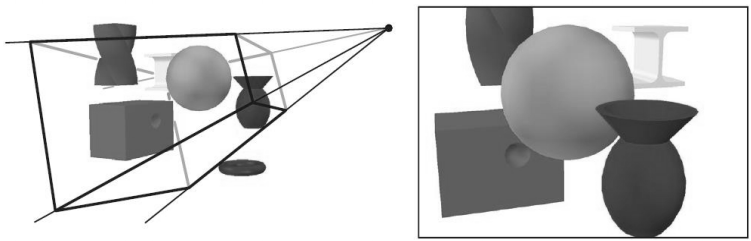
\includegraphics[width=0.9\linewidth]{images/chapter_stato_arte/stato_arte_rendering_3d.png}\hfill
 \caption[Rendering 3D]{A sinistra una scena 3D, a destra un render 2D}
 \label{fig:stato_arte_rendering_3d}
\end{figure}
\\
In un ambiente grafico 3D è possibile pre-rendirizzare una scena (pre-rendering) o renderizzarla in tempo reale (real-time rendering).
\\
Il rendering real time permette la generazione di un flusso di immagini intervallate da brevi istanti di tempo.
È un processo interattivo in quanto ogni immagine da esso generata rappresenta il feedback dell’interazione dell’osservatore con l’immagine precedente.
\\ 
Si viene a creare un ciclo che prevede il rendering e l’interazione con l’immagine renderizzata, e ciò avviene con una velocità tale per cui l’osservatore non vede le singole immagini, ma un unico processo dinamico.
\\ 
La rapidità con cui le immagini vengono mostrate su schermo è misurata in frame per secondo (FPS): maggiore è l’FPS, minore è il tempo di risposta ad un azione dell’osservatore, migliore è l’interattività.
\\ 
Allo stato attuale, il rendering in real-time è possibile grazie all’esistenza di componenti hardware dedicate all’accelerazione grafica: le unità di processamento grafico, o GPU. 
Esse sono in grado di gestire, ad ogni frame, milioni se non miliardi di pixel. 
\\
Tuttavia è importante sottolineare il fatto che il rendering real-time produce risultati qualitativamente peggiori rispetto ad un rendering off-line (o pre-rendering), anche se il divario tra i due tende ad assottigliarsi. 
\\

Il pre-rendering è il processo nel quale le immagini da mostrare non vengono renderizzate in tempo reale dall’ hardware che lo effettua. Piuttosto esse vengono renderizzate precedentemente da un hardware differente, tipicamente più potente di quello utilizzato, e poi proiettate su schermo.
\\
Il processo di fatto permette di diminuire enormemente il carico di lavoro della macchina addetta alla riproduzione video, in quanto essa si limita solamente a mostrare immagini pre-calcolate da un’ altra macchina senza effettuare alcun calcolo di rendering.
\\
Ne consegue un processo computazionalmente oneroso per l’ hardware che lo effettua ma molto efficiente per la macchina che riproduce il video, permettendole di utilizzare modelli grafici più complessi di quelli che sarebbe riuscita a renderizzare in real-time.
\\
I primi impieghi di questa tecnica risalgono all’ inizio degli anni 90 per permettere realizzazioni grafiche ad altissimo livello di realismo, nettamente superiore a quella ottenibile in real-time, e viene utilizzata ancora oggi principalmente per la creazione di film o videogiochi.
Nel 1991 nacquero i primi videogiochi che ne facevano uso, e già nel 1995 venne creato il primo film 3D completamente prerenderizzato: Toy Story.
In quegli anni la grafica pre-renderizzata nei giochi era utilizzata principalmente per la realizzazione di cut-scene fotorealistiche e sfondi prerenderizzati.
\\
Videogiochi come Resident Evil e Final Fantasy sulla prima Playstation fecero largo uso di questa tecnica e contribuirono a renderla famosa fino all’inizio degli anni 2000. 
Verso la fine degli anni 90 questa tecnica ha permesso di ottenere enormi miglioramenti grafici; la figura mette in comparazione un’ immagine che fa utilizzo di sfondi prerenderizzati con una renderizzata in tempo reale.
\\
\begin{figure}[htb]
 \centering
 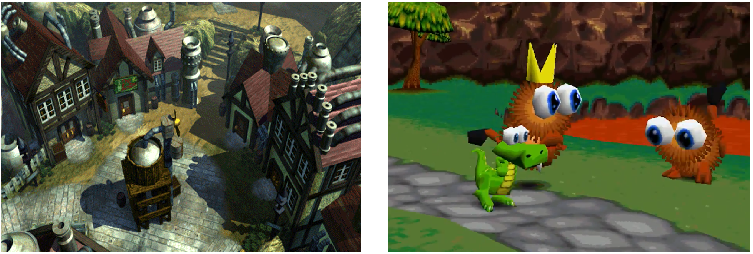
\includegraphics[width=1\linewidth]{images/chapter_stato_arte/stato_arte_croc_ffvii.png}\hfill
 \caption[Confronto tra scena prerenderizzata e real time]{A sinistra una scena prerenderizzata (Final Fantasy VII, 1997), a destra una scena renderizzata in tempo reale (Croc, 1997)}
 \label{fig:stato_arte_confronto_ffvii_croc}
\end{figure}
\\
Lo svantaggio derivante dall’utilizzo di sfondi prerenderizzati risiede però nel basso livello di interattività del personaggio giocante con la scena.
\\
Lo sfondo (o scena) infatti rimane fisso, in quanto l’hardware su cui viene eseguito il gioco non effettuare calcoli real-time ma mostra solamente l’immagine di rendering ottenuta da un hardware molto più potente.
\\
Questo comporta l’impossibilità di muovere la telecamera a proprio piacimento all’interno della scena, cosa possibile invece con il rendering real-time. La camera risulta infatti immobile e permette solamente di osservare la scena dal medesimo punto di osservazione con cui è stata renderizzata dall’hardware più potente. Di fatto è come se l’hardware meno potente mostrasse una fotografia scattata dall’hardware più potente.
\\
Il prerendering inoltre rende impossibile modificare le ombre e le luci dello sfondo in quanto anch’esse rimangono fisse; solamente un approccio real-time permette di calcolarle e quindi modificarle dinamicamente.
\\
Con l’aumentare della potenza degli hardware disponibili sul mercato però già dopo i primi anni 2000 l’utilizzo degli sfondi prerenderizzati è iniziato a diminuire. Le nuove macchine hanno permesso infatti la creazione di convincenti scene 3D in real-time.
\\ 
Nei giorni d’oggi la maggior parte dei giochi sono quasi interamente realizzati tramite rendering real-time. A differenza però degli sfondi prerenderizzati che sono stati completamente abbandonati, i filmati prerenderizzati vengono ancora ampiamente creati, nonostante la differenza con quelli real-time si sia molto assottigliata (\ref{fig:stato_arte_cutscenes}).
\\
\begin{figure}[htb]
 \centering
 
\includegraphics[width=1\linewidth]{images/chapter_stato_arte/stato_arte_tw.png}\hfill
 \caption[Confronto tra cutscene moderne prerenderizzate e real time]{A sinistra una cutscene prerenderizzata, a destra una cutscene renderizzata in tempo reale (The Witcher 3,  2015)}
 \label{fig:stato_arte_cutscenes}
\end{figure}
\\
Attualmente, nonostante la grafica sia quasi completamente real-time, vengono utilizzati differenti metodi di pre-rendering  che alleggeriscono il carico di lavoro del rendering real-time. Metodi quali ad esempio le lightmap che permettono l’utilizzo di luci ed ombre precalcolate, non richiedendo di doverle calcolare real-time, o le env-map precomputate che permettono di alleggerire il carico di lavoro dovuto al calcolo di superfici riflettenti o rifrangenti.
\\
Proprio queste due tecniche, che saranno analizzate nel dettaglio successivamente, vengono utilizzate in questo lavoro di tirocinio per permettere la fruizione di ambienti fotorealistici anche su hardware con prestazioni non elevate. 
\\
Nel presente lavoro di tesi viene utilizzato un approccio misto di prerenderizzazione unito ad una renderizzazione real-time.
Il rendering real-time risulta necessario per permettere il movimento della camera all’interno della scena, inoltre la precomputazione permette il calcolo offline delle informazioni di luce tramite l’utilizzo di un hardware estremamente performante.

\section{Rendering pipeline}
\label{sec:chapter_stato_arte_rendering_pipeline}

Il processo di generazione di immagini 2D dato un insieme di oggetti 3D, delle fonti di luce, e delle texture, si decompone in una successione di passi di elaborazione; tale successione è detta pipeline di rendering. Nella visione più elementare di questa pipeline è possibile individuare tre fasi: Applicazione, Geometria, Rasterizzazione.
Ognuna di queste fasi è essa stessa una pipeline i cui passi possono essere parallelizzati, o anch’essi messi in pipeline. La velocità complessiva del processo viene determinata dal passo più lento della pipeline, ed è espressa in immagini renderizzate per secondo (FPS).

A differenza delle vecchie pipeline di rendering, dove tutto il processo viene eseguito sulla CPU, l’odierna fruibilità di un hardware dedicato all’accelerazione grafica consente di spostare su di esso l’esecuzione di alcuni passi. Infatti, mentre lo stadio Applicazione è sviluppato interamente in software e fatto girare sulla CPU, gli stadi Geometria e Rasterizzazione sono eseguiti sull’unita di processamento grafico (GPU).

\begin{figure}[htb]
 \centering
 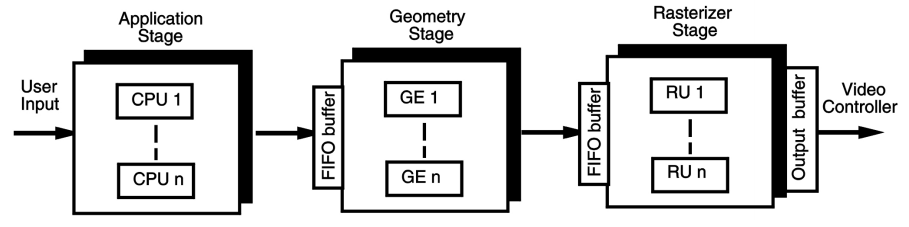
\includegraphics[width=1.0\linewidth]{images/chapter_stato_arte/stato_arte_pipeline.png}\hfill
 \caption[Pipeline di rendering]{Pipeline di rendering}
 \label{fig:stato_arte_pipeline}
\end{figure}

Il livello applicazione è quello più flessibile; infatti lo sviluppatore ne ha pieno controllo, e ne può modificare l’implementazione. I cambiamenti fatti a questo livello possono incidere sulle performance dei livelli che seguono. 
Questa prima fase ha due compiti fondamentali: gestire gli input che possono provenire da più sorgenti, come tastiera o mouse, ed inviare allo step successivo la posizione della camera, le informazioni sulle luci presenti nella scena, e le primitive di rendering; quest’ ultime rappresentano la descrizione in punti, spigoli e triangoli, delle entità geometriche presenti nella scena e sono il dato di input fondamentale per gli hardware grafici. 
Come esempio pratico si può fare riferimento all’editor che verrà mostrato più avanti in questo elaborato: tale strumento consente di selezionare e muovere oggetti o parti di esso; in questo caso il livello Applicazione si occupa di tradurre il movimento del mouse nella corrispondente matrice di rotazione da applicare all’oggetto che si è scelto di ruotare. Inoltre questo livello si occuperà, ad ogni ciclo di rendering, di inviare allo stadio Geometria la posizione della camera, le informazioni sulle luci, e le primitive di rendering dei modelli presenti nella scena.\\

Il livello Geometria è dove vengono effettuate la maggior parte delle operazioni su vertici e triangoli. A differenza del livello Applicazione, questo secondo stadio si può decomporre in una successione di sotto-processi:
Inizialmente ad ogni oggetto della scena è associato un sistema di riferimento in coordinate modello, rispetto al quale l’oggetto appare immobile. Per posizionare ed orientare ogni oggetto nello stesso sistema di riferimento, è necessario applicare ad ognuno una trasformazione del modello, la quale opererà sui vertici e sulle normali di questo per posizionarlo nel sistema di riferimento in coordinate mondo, unico per ogni modello, rispetto al quale gli oggetti appariranno posizionati ed orientati in base alle trasformazioni di modello applicate. Siccome al processo di render partecipano solo gli oggetti che la camera vede, bisogna applicare un’ulteriore trasformazione alla camera e a tutti i modelli della scena. Tale trasformazione porta tutti gli oggetti della scena da un sistema di riferimento in coordinate mondo, ad uno in coordinate camera. In questo nuovo sistema di riferimento la camera è posizionata nell’origine, e punta verso le z negative, con l’asse y che punta verso l’alto, e l’asse x orientata verso destra. Entrambe le trasformate mostrate sono implementate mediante una matrice 4x4. 

\begin{figure}[htb]
 \centering
 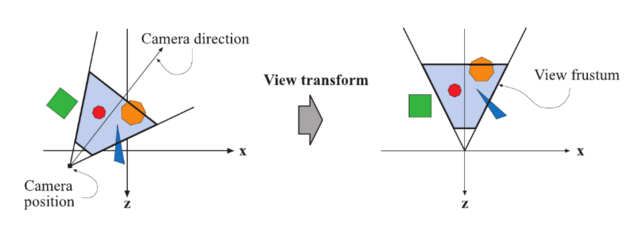
\includegraphics[width=1.0\linewidth]{images/chapter_stato_arte/stato_arte_view_transform.png}\hfill
 \caption[Trasformazione della vista]{Trasformazione della vista}
 \label{fig:stato_arte_trasfvista}
\end{figure}

Forma e posizione degli oggetti non sono l’unico aspetto chiave per un rendering realistico; infatti anche le informazioni sui materiali di ogni oggetto, così come l’effetto di ogni fonte luminosa nella scena, risultano fondamentali. 
Il processo di determinazione di un effetto luminoso su di una superficie composta da un certo materiale è detta shading. Tale processo consiste nel calcolo di una equazione di shading in corrispondenza dei vertici dell’oggetto; ogni vertice può memorizzare diverse informazioni, come la posizione dello stesso, una normale, un colore, o qualsiasi altra informazione necessaria al calcolo dell’equazione, il cui risultato può essere, ad esempio, un colore, un vettore o una coordinata di una texture. E’ importante che il calcolo delle equazioni di shading venga fatto in un sistema di riferimento comune a tutti gli oggetti, in modo che le relazione tra oggetti, camera, e luci, siano preservate. 
Dopo lo shading, il processo di rendering si occupa della trasformazione del volume di vista percepito dalla camera, in un cubo unitario detto volume di vista canonico.
Tipicamente vengono usati due metodi di proiezione: ortografica e prospettica.
In quella ortografica il volume di vista appare come un parallelepipedo rettagolo, e la proprietà fondamentale è che le linee parallele rimangono tali dopo la trasformazione.
Nella proiezione prospettica invece viene simulato il modo in cui noi percepiamo la dimensione degli oggetti: tanto più un oggetto si allontana dalla camera, tanto più sarà piccolo dopo la proiezione. In questo caso le linee parallele convergono all’orizzonte, e il volume di vista è rappresentato come una piramide tronca con base rettangolare.
Un oggetto che subisce una delle due proiezioni  si dice appartenente al sistema di riferimento con coordinate normalizzate della camera. 

\begin{figure}[htb]
 \centering
 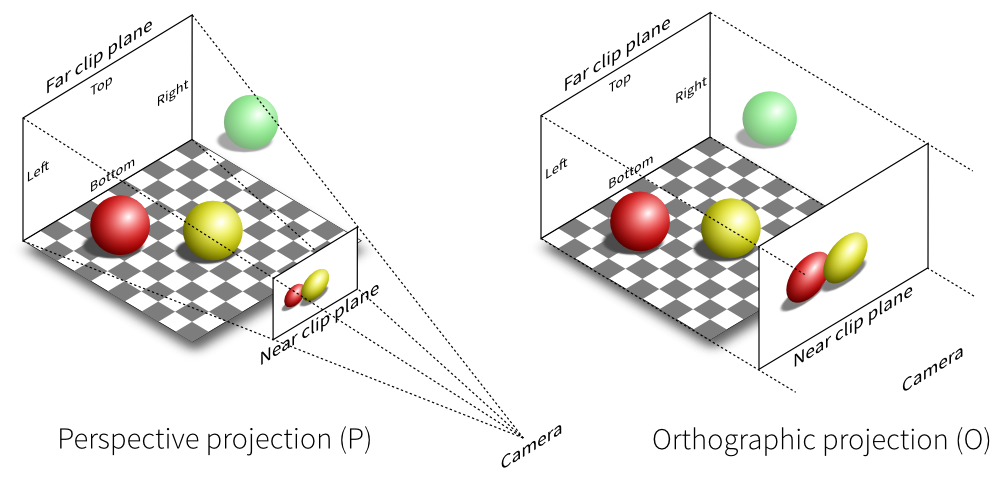
\includegraphics[width=1.0\linewidth]{images/chapter_stato_arte/stato_arte_projections.png}\hfill
 \caption[Proiezione prospettica ed ortogonale]{Volume di vista nella proiezione ortografica (a sinistra), e prospettica (a destra)}
 \label{fig:stato_arte_trasfvista}
\end{figure}

A questo punto, dato un volume di vista, sappiamo quali sono le primitive di rendering da dare in pasto alla fase di rasterizzazione, dove verrano finalmente disegnate su schermo.
Se una primitiva risiede all’interno del volume passerà allo stadio successivo, così come verrà ignorata se presente al di fuori di esso. Per quanto riguarda le primitive che si trovano parzialmente all’interno del volume di vista c’è bisogno di un ulteriore passo di elaborazione, detto clipping. La trasformazione in coordinate camera, e la proiezione, fanno si che il clipping possa essere fatto con riferimento ad un volume di vista rappresentato da un cubo unitario: questo vuol dire che che se ad esempio abbiamo un spigolo con un vertice nel volume di vista e con l’altro fuori, è sufficiente calcolare un nuovo vertice nell’intersezione tra lo spigolo ed il cubo unitario, scartando così il vertice esterno.\\

\begin{figure}[htb]
 \centering
 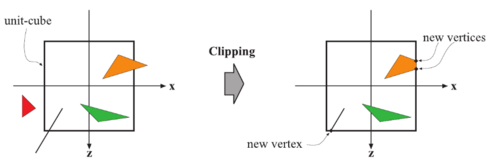
\includegraphics[width=1.0\linewidth]{images/chapter_stato_arte/stato_arte_clipping.png}\hfill
 \caption[Clipping]{Clipping}
 \label{fig:stato_arte_clipping}
\end{figure}

A questo punto le primitive nel volume di vista, le quali sono ancora descritte in coordinate a tre dimensioni, sono passate alla fase di mappatura su schermo. 
Nella mappatura le coordinate x,y di ogni primitiva sono trasformate in coordinate di schermo, mentre la z non subisce alcuna mappatura.
Le coordinate di schermo insieme alla z costituiscono le coordinate di finestra, le quali vengono passate alla fase di rasterizzazione.

\begin{figure}[htb]
 \centering
 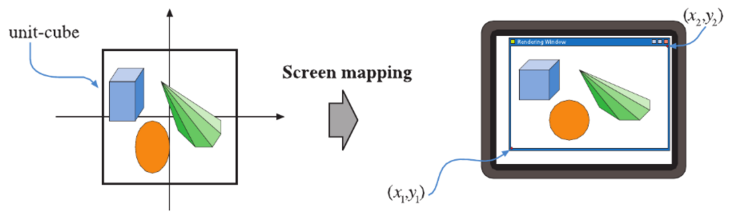
\includegraphics[width=1.0\linewidth]{images/chapter_stato_arte/stato_arte_mapping.png}\hfill
 \caption[Mappatura su schermo]{Mappatura su schermo delle primitive nel volume di vista}
 \label{fig:stato_arte_mapping}
\end{figure}

A questo punto le coordinate di finestra, insieme alle informazioni di shading associate ad ogni vertice, vengono convertite in pixel sullo schermo. Anche qui, come nella fase Geometria, si può decomporre il processo in più passi:

Vi è una fase iniziale di computazione di informazioni necessarie alla fase successiva; tali informazioni saranno utili, ad esempio, per l’interpolazione dei dati di shading computati nella fase Geometria.
Per ogni pixel vengono individuati dei frammenti, ovvero porzioni di pixel posizionate all’interno di un triangolo. Le proprietà di ogni frammento sono generate mediante interpolazione dei dati memorizzati sui vertici del triangolo di cui fa parte. 
Tali proprietà includono:

\begin{itemize}
\item Profondità del frammento: l’interpolazione della coordinata (di finestra) z sui vertici del triangolo di cui il frammento fa parte;
\item Dati di shading calcolati nella fase Geometria;
\end{itemize}

I dati di shading interpolati sono necessari al calcolo dello shading sui frammenti di pixel, il cui risultato è un colore da dare in input alla fase successiva.
In quest’ultima fase del processo di rasterizzazione vengono dapprima memorizzate le informazioni di ogni pixel in un buffer di colori, detto pixel buffer, ovvero un array dove ogni elemento è un pixel con un informazione a 3 componenti di colore: rosso, verde e blu.
A questo punto il colore ottenuto dallo shading sui frammenti di pixel ed il colore memorizzato nel buffer sono combinati.
Tale buffer deve contenere il colore relativo alle primitive di scena visibili dal punto di vista della camera. 
Per individuare quali oggetti sono visibili e quali non lo sono all’interno della scena viene fatto uso di un ulteriore buffer, detto z-buffer. Questo buffer ha stesse dimensioni e forma del pixel buffer, e per ogni pixel viene memorizzata la distanza tra la camera e la primitiva di rendering più vicina ad essa. Il funzionamento dello z-buffer è il seguente: 
Quando una primitiva deve essere renderizzata su un determinato pixel, il valore z tra la primitiva e il pixel del piano immagine della camera viene confrontato con quello memorizzato nello z buffer:

\begin{itemize}
\item Se il nuovo valore z è più piccolo di quello memorizzato nel buffer, allora la nuova primitiva è più vicina alla camera di quanto lo fosse quella relativa al valore di z memorizzato nel buffer. A questo punto vengono aggiornati z-buffer e pixel buffer, entrambi nella stessa posizione: il primo con il nuovo valore z, il secondo con il colore relativo alla nuova primitiva da renderizzare. 
\item Se invece il nuovo valore z è più grande di quello memorizzato nel buffer, non vi è alcun aggiornamento.
\end{itemize}

\begin{figure}[htb]
 \centering
 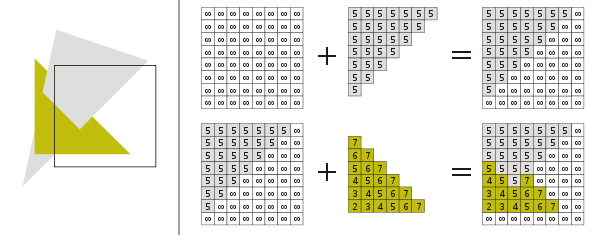
\includegraphics[width=1.0\linewidth]{images/chapter_stato_arte/stato_arte_z_buffer.png}\hfill
 \caption[Z-buffer]{Z-buffer}
 \label{fig:stato_arte_z_buffer}
\end{figure}


\section{Ray Tracing}
\label{sec:chapter_stato_arte_ray_tracing}

In computer grafica, ray tracing è una tecnica di rendering che permette di generare un’ immagine tracciando la direzione della luce attraverso ogni pixel della scena da renderizzare.
Essa viene utilizzata per determinare quali oggetti sono visibili dall’ osservatore, ovvero la camera, e quali di questi sono illuminati o in ombra. \cite{rayt1}
\\
Il meccanismo base è semplice, vengono lanciati dei raggi (view ray) da ogni pixel del piano immagine, che rappresenta l’immagine a due dimensioni dell’ ambiente osservato dalla camera, verso la scena.
\\ 
Per ogni raggio lanciato viene calcolato l’oggetto più vicino a partire dall’ osservatore. Dall’oggetto viene lanciato un nuovo raggio (shadow ray) verso ogni luce e viene valutata la presenza di un altro oggetto tra i due.
Se tale oggetto è presente ed è opaco, allora la luce viene bloccata, se invece è trasparente la luce viene attenuata.
\\
Se tale oggetto è assente allora l’ oggetto intersecato dal primo raggio viene colpito dalla luce.
Quindi il colore di uno specifico pixel da mostrare sul piano immagine viene calcolato in base al colore ed alle proprietà del materiale del primo oggetto intersecato dal view ray, insieme alla quantità di luce che quel pixel riceve dalle luci presenti nella scena, calcolate grazie agli shadow ray.
\\
\begin{figure}[htb]
 \centering
 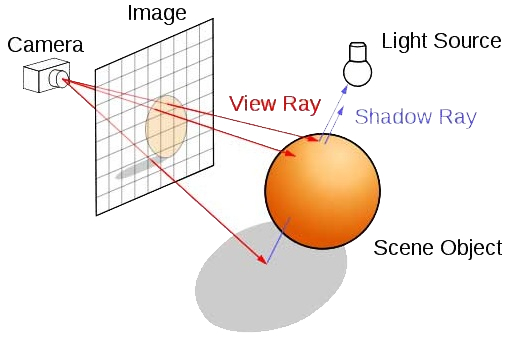
\includegraphics[width=0.7\linewidth]{images/chapter_stato_arte/stato_arte_raytracing_shadowray.jpg}\hfill
 \caption[Ray tracing e shadow ray]{Algoritmo di ray tracing, ed utilizzo dello shadow ray}
 \label{fig:stato_arte_raytracing_shadowray}
\end{figure}
\\
Altri raggi possono essere lanciati dall’ oggetto intersecato dal view ray in maniera tale da consentire la crazione di un’effetto di riflessione e/o rifrazione.
Se l’ oggetto intersecato è ad esempio riflettente, un raggio può essere generato verso la direzione di riflessione.
\\
Questo raggio prende il colore del primo oggetto intersecato. Dal punto appena intersecato viene nuovamente lanciato il ray shadow insieme ad un’ulteriore raggio nella direzione di riflessione e/o rifrazione, a seconda del fenomeno provocato dall’oggetto colpito. 
\\Questo procedimento viene ripetuto ricorsivamente fino a quando una superficie non riflettente viene colpita o fino quando il contributo massimo di rimbalzi non viene raggiunto.
\\
Se l’ oggetto intersecato è solido e trasparente, un nuovo raggio può essere generato nella direzione di rifrazione, ed esattamente come per la riflessione questo verrà valutato ricorsivamente.
\\
\begin{figure}[htb]
 \centering
 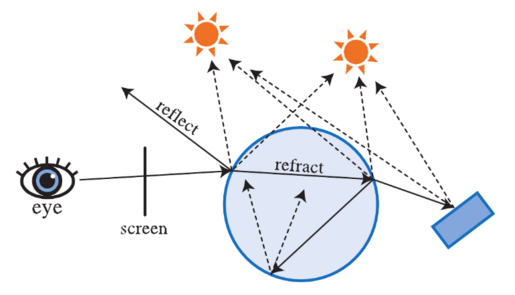
\includegraphics[width=0.7\linewidth]{images/chapter_stato_arte/stato_arte_refr_refl.png}\hfill
 \caption[Ray tracing ed effetti di rifrazione/riflessione]{Algoritmo di ray tracing e gestione degli effetti di rifrazione e riflessione}
 \label{fig:stato_arte_refr_refl}
\end{figure}
\\
Il problema principale è il fatto che, oltre alle sorgenti luce, ogni singolo oggetto visibile ad occhio nudo riflette luce ed il 
ray tracing calcola solamente le luci dirette alle superfici mentre quelle indirette vengono completamente ignorate. L’ algoritmo di path tracing risolve questa limitazione. \cite{path_ray}

\section{Path Tracing}
\label{sec:chapter_stato_arte_path_tracing}

In computer grafica, path tracing è una tecnica di rendering che fornisce una soluzione molto più realistica al problema del calcolo della luce rispetto al ray casting.
Il rendering che si ottiene mediante questo algoritmo è una vera simulazione di come la luce percorre la scena e non solamente una approssimazione artistica. Permette di simulare effetti quali ad esempio luci indirette come la luce che rimbalza da una superficie (Fig. \ref{fig:stato_arte_luci_dir_ind}), ombre leggere ed effetti caustici (Fig. \ref{fig:stato_arte_ombre_caust}) 
\\
\begin{figure}[htb]
 \centering
 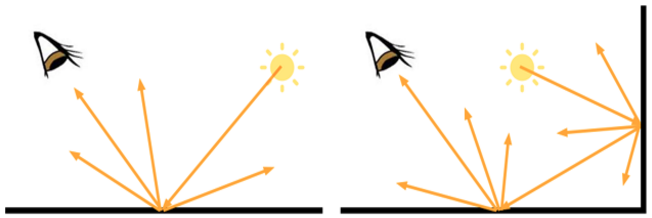
\includegraphics[width=0.8\linewidth]{images/chapter_stato_arte/stato_arte_luci_dir_ind.png}\hfill
 \caption[Illuminazione diretta e indiretta]{Confronto tra illuminazione diretta (a sinistra) e indiretta (a destra)}
 \label{fig:stato_arte_luci_dir_ind}
\end{figure}
\\
\begin{figure}[htb]
 \centering
 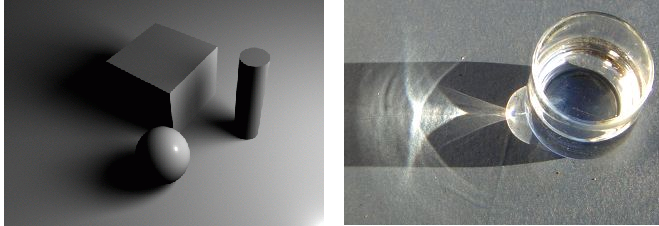
\includegraphics[width=0.8\linewidth]{images/chapter_stato_arte/stato_arte_ombre_caust.png}\hfill
 \caption[Ombreggiature ed effetti caustici]{Una scena con delle ombre leggere (a sinistra), ed effetti caustici nella realtà (a destra)}
 \label{fig:stato_arte_ombre_caust}
\end{figure}

L’ approccio utilizzato prevede di lanciare raggi a partire dalla camera virtuale verso la scena. 
A differenza del ray tracing però, quando un raggio colpisce una superficie, ne viene calcolato il rimbalzo ottico randomico e quindi creato un  nuovo raggio nella direzione calcolata. 
La creazione di nuovi raggi in base ai rimbalzi continua fino a quando non viene colpita una fonte di luce o non si raggiunge una soglia massima di rimbalzi.
Questo algoritmo permette di ottenere un’ approssimazione fisica molto realistica delle fonti luminose che nel mondo reale  proiettano raggi di luce che rimbalzano tra oggetti, cambiando colore ed intensità fino a quando non raggiungono l’ occhio (la camera in questo caso). 
Il processo appena descritto viene simulato dal path-tracing; l’unica differenza è che i raggi vengono tracciati al contrario, dalla camera alla scena. Questo perchè, se venissero lanciati raggi di luci a partire dalle fonti luminose, verrebbere inutilmente calcolata una moltitudine di raggi che non raggiungerebbero mai la camera, non contribuendo in alcun modo all’ immagine finale.
Questo provoca un incremento delle prestazioni dell’ algoritmo ma provoca anche alcune imprecisioni nel calcolo delle luci, soprattutto quando vengono lanciati pochi raggi nella scena. 
L’ algoritmo ricorsivo nel dettaglio è il seguente:
\begin{itemize}
\item Per ogni pixel p del piano immagine della camera viene lanciato un raggio nella scena.
\item Viene calcolata e salvata la direzione del nuovo raggio in base al rimbalzo ottico che effettua sull’ oggetto intersato. La direzione viene calcolata secondo una funzione randomica che tiene conto del materiale colpito.
\item Viene calcolata la radianza nel punto intersecato, cioè la quantità di luce ricevuta,  tramite una specifica funzione pesata che tiene in considerazione l’attenuazione della radianza in base ai rimbalzi. Per effettuare il calcolo è però necessaria l’informazione della quantità di luce ricevuta nel punto di intersezione, quantità ottenuta dal risultato della chiamata ricorsiva dell’ algoritmo sul nuovo raggio.
\item Viene chiamata la funzione ricorsiva e si ricomincia con il punto due fino a quando:
\begin{itemize}
\item Una fonte di luce viene colpita; in tal caso la chiamata ricorsiva ritorna la luce emessa dalla luce.
\item Una soglia massima di rimbalzi è raggiunta oppure il raggio lascia la scena, ad esempio colpendo lo sfondo; in tal caso nessuna luce è emessa e viene tornato nero.
\end{itemize}
\end{itemize}

Quindi se il raggio colpisce una fonte di luce, la radianza emessa viene distribuita su ogni punto di intersezione colpito dal raggio secondo una specifica funzione pesata che tiene conto del fenomeno fisico dei rimbalzi. 
Nell’ algoritmo appena proposto per ogni pixel del piano immagine della camera viene lanciato un solo raggio che rimbalza nella scena. Di norma però per ogni pixel vengono lanciati un numero elevato di raggi, equivalente al numero di sample scelto. Il sample indica il numero di raggi da lanciare per ogni pixel del piano immagine.
Quando però questo numero è basso è possibile ottenere con una elevata probabilità una scena rumorosa (figura a sinistra) in quanto da ogni pixel partono pochi raggi di luce. 
Siccome i raggi lanciati quando intersecano un oggetto rimbalzano in una direzione randomica dipendente dal materiale colpito, è molto probabile che questi non colpiscano la fonte di luce che invece dovrebbe illuminare il pixel, producendo di fatto un pixel nero invece che colorato. 
Lanciando quindi pochi raggi per ogni pixel del piano immagine, la probabilità che per quel pixel siano conteggiate nel calcolo tutte le fonti da cui riceve la luce è bassa. 
Molto probabile invece è che per alcuni pixel non vengano conteggiate delle luci, che invece verranno conteggiate per altri pixel. Questo provoca rumore nell’ immagine renderizzata. 
Il rumore è facilmente identificabile dall’ alternanza continua di pixel illuminati diversamente, ma che in realtà dovrebbero avere un’illuminazione identica.
Maggiore è il sample, quindi, maggiore è la probabilità che per quel pixel vengano conteggiate tutte le fonti di luce che riceve \ref{fig:stato_arte_effetto_sampling} .
\\
\begin{figure}[htb]
 \centering
 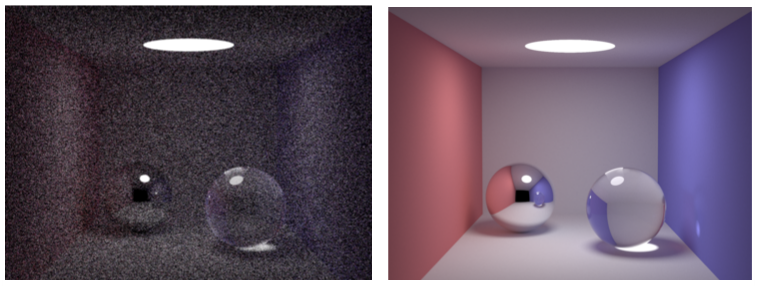
\includegraphics[width=0.8\linewidth]{images/chapter_stato_arte/stato_arte_effetto_sampling.png}\hfill
 \caption[Illuminazione al variare dei sample]{Illuminazione al variare dei sample: confronto tra render con basso valore di sample (a sinistra), e alto valore di sample (a destra).}
 \label{fig:stato_arte_effetto_sampling}
\end{figure}

È chiaro quindi quanto questo algoritmo sia computazionalmente oneroso, permettendo di ottenere risultati corretti solamente con sample alto. Maggiore è il sample, maggiore è il tempo di attesa per il completamento del rendering, migliore è il risultato dell’ illuminazione globale della scena ottenuta.
Oltre a quella appena descritta, esistono diverse implementazioni del path tracing, che permettono di ottenere alcuni vantaggi in determinate situazioni.
Un approccio prevede, quando un raggo colpisce una superficie, di lanciare un nuovo raggio sia nella direzione di rimbalzo che verso le funti di luce dirette.
\\
\begin{figure}[htb]
 \centering
 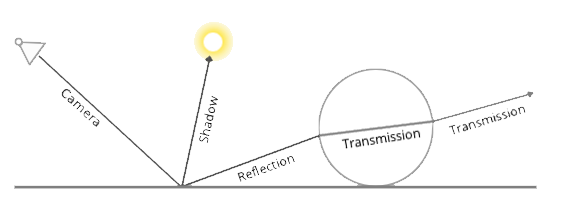
\includegraphics[width=0.8\linewidth]{images/chapter_stato_arte/stato_arte_path_alt.png}\hfill
 \caption[Path Tracing: implementazioni alternative]{Approccio utilizzato da un'implementazione alternativa dell'algoritmo di path tracing.}
 \label{fig:stato_arte_path_alt}
\end{figure}

Questa implementazione permette di ottenere in scene con poche luci indirette risultati di rendering con basso o impercettibile rumore anche con sample basso. 
Blender utilizza questo approccio con il suo Cycles Render, che verrà spiegato nei capitoli successivi.



\section{Lightmap}
\label{sec:chapter_stato_arte_lightmap}

Le lightmap sono strutture dati identiche a normali texture ma, mentre quest’ultime sono array di elementi d’immagine chiamati texels, le lightmap sono array di elementi di luce , o irradianza, detti lumels. Questi elementi di luce vengono pre-computati offline.
Il fattore scala di un lumel definisce la risoluzione della lightmap: ad esempio un fattore scala 16 indica che il lumel ha un fattore scala 16:1 rispetto all’unità geometrica usata dal sistema per misurare distanze o definire coordinate. 
Un fattore scala 1 indica invece che il lumel è grande esattamente quanto un unità geometrica. 
\\
\begin{figure}[htb]
 \centering
 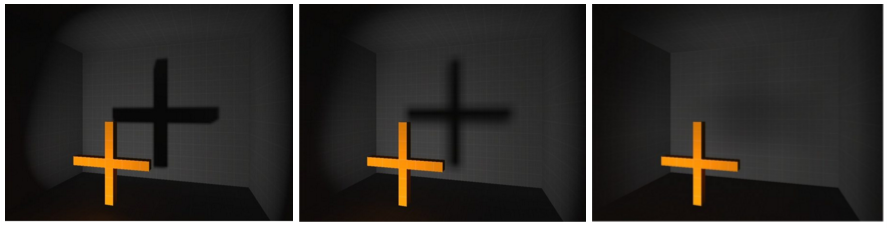
\includegraphics[width=1\linewidth]{images/chapter_stato_arte/stato_arte_scale_shadow.png}\hfill
 \caption[Fattore scala lumel]{Effetto dell'aumento del fattore scala dei lumel sulla risoluzione dell'ombra (da sinistra verso destra).}
 \label{fig:stato_arte_scale_shadow}
\end{figure}

Diminuendo il fattore scala aumenta la definizione della lightmap ma aumenta anche lo spazio occupato in memoria, peggiorando le prestazioni del rendering; per questo i grafici 3D spesso devono giungere a compromessi tra performance e qualità.
Il mapping di una lightmap o di una texture, su di una superficie 3D avviene nello stesso modo: il processo, detto di texturizzazione, inizia individuando un punto nello spazio definito in coordinate modello; si sceglie questo sistema di riferimento in modo che la texture rimanga mappata sulla superficie sempre nello stesso modo, anche se la superficie si dovesse spostare. \\
Dopodichè il vettore con le tre coordinate del punto viene proiettato in un vettore a due coordinate (u,v), avente ognuna un valore compreso nell’intervallo tra 0 e 1. Questi due valori sono moltiplicati per la risoluzione della texture, o della lightmap, ottenendo così la posizione del texel, o lumel, da mappare sul punto individuato nello spazio del modello.
\\
\begin{figure}[htb]
 \centering
 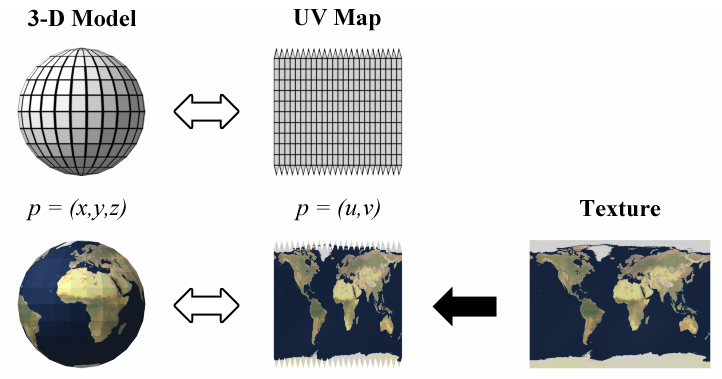
\includegraphics[width=0.6\linewidth]{images/chapter_stato_arte/stato_arte_uvmap.png}\hfill
 \caption[Texturizzazione mediante mappa UV]{Processo di texturizzazione di un oggetto.}
 \label{fig:stato_arte_uvmap}
\end{figure}
\\
Quando viene creata una lightmap per ogni oggetto della scena, tipicamente ogni oggetto avra due texture: una texture diffuse che definisce il colore principale della superficie 3D, ed una lightmap con i valori di luce e ombra proiettati sull’oggetto della scena; quest’ultime tipicamente sono in bianco e nero, a meno che non vi sia del colore proveniente dalla luce stessa, o da un oggetto riflettente. 
\\
Per ogni oggetto è possibile sommare lightmap e diffuse texture, moltiplicando i valori di irradianza della lightmap per i valori RGB della diffuse texture; in questo modo è possibile memorizzare un unica texture al posto di due. Anche se dal punto di vista del consumo di memoria è una soluzione vantaggiosa, ci sono comunque degli aspetti per cui vale la pena tenere separate le due mappe, primo fra tutti la riusabilità della diffuse texture.
\\
Questa infatti è decisamente più riusabile di una lightmap, ad esempio è possibile ripetere una diffuse texture su di una superficie 3D. Sommando la diffuse ad una lightmap si perderebbe questo vantaggio. Inoltre in presenza di due scene identiche, una vista di giorno, l’altra di notte, è possibile generare due lightmap diverse mantenendo la stessa diffuse map.
\\
\begin{figure}[htb]
 \centering
 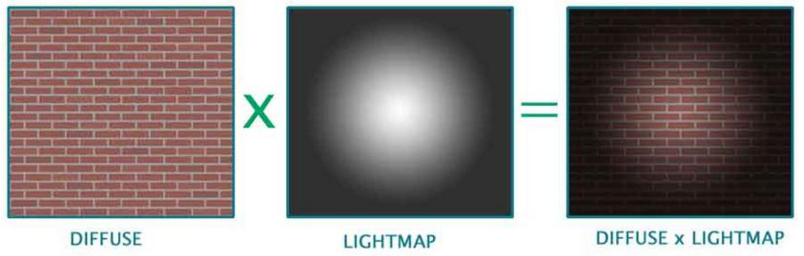
\includegraphics[width=0.9\linewidth]{images/chapter_stato_arte/stato_arte_diffuse_lightmap.png}\hfill
 \caption[Combinazione texture/lightmap]{Combinazione di una diffuse texture con una lightmap.}
 \label{fig:stato_arte_diffuse_lightmap}
\end{figure}
\\
\subsection{Baking delle lightmap}
\label{sec:chapter_stato_arte_baking_lightmap}

Il processo di precomputazione delle informazioni di luce all’interno di una scena con oggetti e luci statiche, e la memorizzazione dei risultati all’interno di una struttura dati del tipo sopra descritto, è detto baking delle lightmap. 
\\
Questo approccio è il migliore se si vogliono sfruttare algoritmi di illuminazione indiretta nelle applicazioni real-time, come i videogiochi. In generale, il baking delle lightmap porta in dote tutta una serie di vantaggi.
A livello qualitativo, il bake permette la fruizione di:
\begin{itemize}
\item Illuminazione indiretta.
\item Rimbalzi multipli.
\item Migliore illuminazione diretta.
\item Una più ampia scelta di sorgenti luminose da inserire nella scena.
\end{itemize}
Per quanto riguarda le performance:
\begin{itemize}
\item Sono elevate a tempo di esecuzione.
\item Non dipendono dal tipo di luce utilizzata.
\item Non dipendono dall’ algoritmo di illuminazione indiretta utilizzato.
\item Sono identiche sia per lightmap di ottima qualità, che di pessima qualità.
\item Permettono di aggiungere alla scena le sorgenti luminose che si desidera.
\item Sono scalabili.
\item Se si eseguisse l’algoritmo in realtime l’angolazione e la posizione delle luci, nonchè la posizione dell’osservatore, inficierebbero sule performance di rendering delle ombre e degli effetti di luce sulla scena.
\end{itemize}
L’intero processo di baking di una lightmap si può scomporre in tre fasi.
\\

La prima fase riguarda il calcolo delle coordinate di texture della lightmap.
In questa fase il modello 2D della lightmap viene proiettato sulla superficie 3D del modello, individuando per ogni poligono della superficie una specifica area della lightmap.
Il processo di mappatura di una texture 2D su una superficie 3D è detto UV mapping.
\newpage
\begin{figure}[htb]
 \centering
 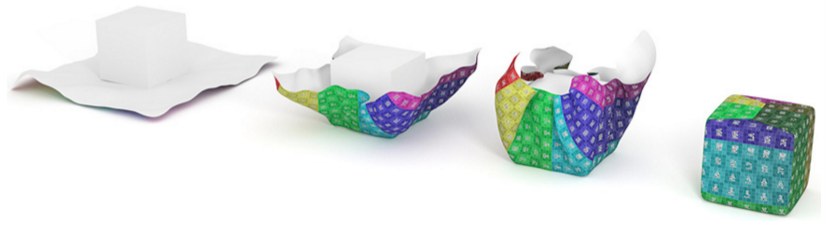
\includegraphics[width=0.9\linewidth]{images/chapter_stato_arte/stato_arte_unwrap.png}\hfill
 \caption[Mappatura delle coordinate UV]{Processo di unwrap (da destra verso sinistra).}
 \label{fig:stato_arte_unwrap}
\end{figure}
Si consideri il seguente esempio per comprendere il processo di UV Mapping.
\\
Si supponga di avere uno scatolone, che può essere visto come un’ oggetto cubico 3D all’interno della scena. 
\\
Aprendo lo scatolone in tutti i punti dove presenta una piega, si ottiene una superficie piana (Fig \ref{fig:stato_arte_unwrap}); questa procedura è detta \emph{unwrap} di un oggetto 3D su di un immagine 2D. Guardando questa superficie si definisce U la direzione destra o sinistra sulla superficie, e V la direzione in alto o in basso sulla stessa. 
\\
Questa superficie viene definita \emph{mappa UV}. U e V sono dette coordinate di texture; (u=0,v=0) indica l’angolo in basso a sinistra della texture, mentre (u=1,v=1) indica l’angolo in alto a destra della stessa. 
\\
Queste coordinate vengono usate al posto della X e Y che invece, insieme alla Z, fanno riferimento alle coordinate nello spazio 3D. Una volta riassemblata la scatola, una qualsiasi posizione (u,v) presente sulla superficie 2D, viene trasformata in una posizione (x,y,z) sulla scatola; questa operazione è detta wrap di un immagine 2D su di un oggetto 3D, e verrà descritto al passo successivo.
\\
Una mappa UV può essere generata dall’applicazione software in modo completamente automatico, semi automatico, o creata a mano dall’artista 3D. Ad esempio utilizzando Blender, 
un software per la computer grafica 3D che verrà esposto in un paragrafo dedicato in quanto punto cardine del presente lavoro di tesi, espone un interfaccia per mezzo della quale poter decidere esattamente come mappare le facce di un oggetto 3D in un immagine 2D. 
\newpage
\begin{figure}[htb]
 \centering
 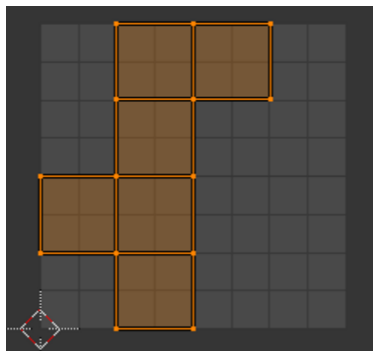
\includegraphics[width=0.5\linewidth]{images/chapter_stato_arte/stato_arte_uvmap_blender.png}\hfill
 \caption[Mappa UV realizzata in Blender]{Una mappa UV realizzata con il software di grafica 3D Blender.}
 \label{fig:stato_arte_uvmap_blender}
\end{figure}
Questa prima fase è fondamentale, perchè senza eseguire l’unwrap dell’oggetto 3D sulla lightmap è impossibile stabilire, dato il valore di radianza di un poligono dell’oggetto 3D, qual’è il lumel corrispondente in cui memorizzarlo.
\\
La seconda fase prevede di calcolare la posizione in coordinate mondo e la normale, per ogni lumel in ogni lightmap.
\\
Ogni lumel di una lightmap deve essere mappato in una posizione nel sistema di riferimento in coordinate mondo. Finchè le geometrie nella scena rimarrano statiche, e la dimensione delle lightmap rimarrà invariata, le corrispondenze tra coordinate texture e coordinate mondo risulteranno invariate, e quindi possono essere preprocessate offline una volta sola e poi riutilizzate.
\\
A questo punto verrà mostrato come, partendo da una mappa UV di un poligono, le posizioni in coordinate texture vengono mappate in posizioni sulla superficie del poligono.
Si consideri il triangolo in figura \ref{fig:stato_arte_ligh_triangle1}.
\\
Come è possibile notare, le componenti per la posizione dei vertici sono vettori 2D e non 3D; il motivo verrà spiegato più avanti.
\newpage
\begin{figure}[htb]
 \centering
 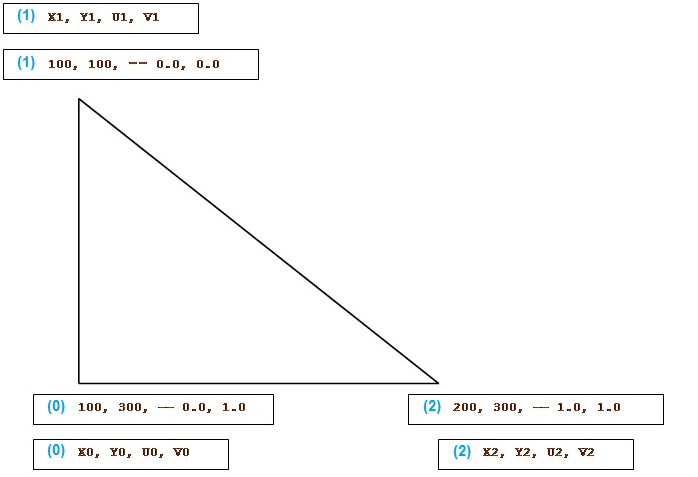
\includegraphics[width=0.7\linewidth]{images/chapter_stato_arte/stato_arte_ligh_triangle1.png}\hfill
 \caption[Triangolo di esempio per mapping UV]{Un triangolo definito all'interno di una mappa UV}
 \label{fig:stato_arte_ligh_triangle1}
\end{figure}
Allo stato attuale i dati in possesso sono:	
\begin{itemize}
\item Le posizioni dei vertici del triangolo nel mondo.
\item Le coordinate texture $(u,v)$ per ognuno dei tre vertici.
\end{itemize}
Dato un punto in coordinate texture interno al poligono in figura \ref{fig:stato_arte_ligh_triangle1}, bisogna ottenere la posizione 2D del triangolo corrispondente nel mondo.
Un modo possibile è sfruttare le derivate per calcolare la variazione delle coordinate mondo $x$ e $y$ in base a come variano le coordinate texture $u$ e $v$; siccome in tutto sono 4 coordinate avremo 4 equazioni così espresse, in base ai vertici del triangolo in figura \ref{fig:stato_arte_ligh_triangle1}:
\\
\begin{equation}
\frac{dx}{du} = \frac{(x_1 - x_2)*(v_0 - v_2) - (x_0 - x_2)*(v_1 - v_2)}{(v_0 - v_2)*(u_1 - u_2) - (v_1 - v_2)*(u_0 - u_2)}
\label{dxdu}
\end{equation}
\begin{equation}
\frac{dx}{dv} = \frac{(x_1 - x_2)*(u_0 - u_2) - (x_0 - x_2)*(u_1 - u_2)}{(v_0 - v_2)*(u_1 - u_2) - (v_1 - v_2)*(u_0 - u_2)}
\label{dxdv} 
\end{equation}
\begin{equation}
\frac{dy}{du} = \frac{(y_1 - y_2)*(v_0 - v_2) - (y_0 - y_2)*(v_1 - v_2)}{(v_0 - v_2)*(u_1 - u_2) - (v_1 - v_2)*(u_0 - u_2)}
\label{dydu}
\end{equation}
\begin{equation}
\frac{dy}{dv} = \frac{(y_1 - y_2)*(u_0 - u_2) - (y_0 - y_2)*(u_1 - u_2)}{(v_0 - v_2)*(u_1 - u_2) - (v_1 - v_2)*(u_0 - u_2)} 
\label{dydv}
\end{equation}
\\
Per la derivazione completa delle quattro equazioni si rimanda a [numero fonte], tuttavia l’idea di base è piuttosto semplice. Osservando la figura \ref{fig:stato_arte_ligh_triangle2} si supponga di dover determinare come varia la coordinata $x$ rispetto alla $u$. Per fare questo si fissa la coordinata $v$ e si muove la $u$. Così facendo viene individuato un nuovo generico punto nello spazio. 
\\
\begin{figure}[htb]
 \centering
 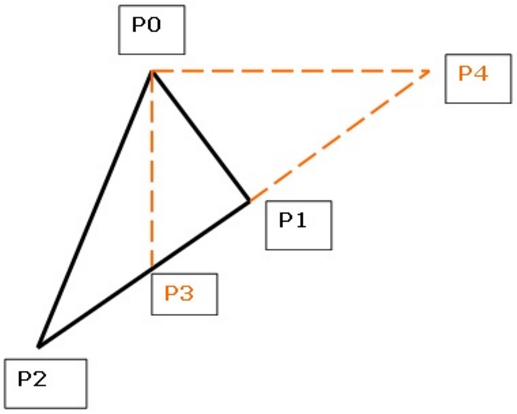
\includegraphics[width=0.5\linewidth]{images/chapter_stato_arte/stato_arte_ligh_triangle2.png}\hfill
 \caption[Triangolo di esempio per calcolo coordinate]{Dal vertice $p_0$ del triangolo in foto, si ottiene il punto $p_4$ mantenendo fissa la coordinata $v$ di $p_0$ e variando la coordinata $u$.}
 \label{fig:stato_arte_ligh_triangle2}
\end{figure}
\\
Dalla figura \ref{fig:stato_arte_ligh_triangle2} si può vedere come, fissando la $v$ e muovendo $p_0$ lungo l’asse delle $u$, si ottiene il punto $p_4$. A questo punto viene calcolata la variazione di $x$ rispetto a $u$ nello spostamento da $p_0$ a $p_4$:
\begin{equation}
\frac{dx}{du} = \frac{(x_4 - x_0)}{(u_4 - u_0)} 
\label{derivata_1}
\end{equation}
Dall'equazione \ref{derivata_1} vengono quindi individuate due componenti: $dx = (x_4-x_0)$ dove l’incognita è $x_4$, e $du = (u_4-u_0)$ dove l’incognita è $u_4$ E’ possibile ottenere queste coordinate di $p_4$ utilizzando l’equazione della retta passante per due punti: costruendo il triangolo come in figura \ref{fig:stato_arte_ligh_triangle2}, la retta passante per $p_1$ e $p_2$ è la stessa che passa per $p_3$ e $p_4$, pertanto è possibile definire le equazioni per due rette: una usando $x_4$ come ingognita, e $x_1,x_2,y_1,y_2,y_4=y_0$ come coordinate note, e l’altra con $u_4$ come incognita e $u_1,u_2,v_1,v_2,v_4=v_0$ come coordinate note:
\begin{equation}
\frac{(x_1 - x_2)}{(y_1 - y_2)} = \frac{(x_4 - x_2)}{(y_4 - y_2)} 
\label{eq_retta1}
\end{equation}
\begin{equation}
\frac{(u_1 - u_2)}{(v_1 - v_2)} = \frac{(u_4 - u_2)}{(v_4 - v_2)} 
\label{eq_retta2}
\end{equation}
A questo punto l’ultimo passaggio consiste nell'esprimere l'equazione \ref{eq_retta1} in funzione di $x_4$, e l'equazione \ref{eq_retta2} in funzione di $u_4$, e sostituirle in \ref{derivata_1}; svolgendo i calcoli si arriva ad una forma equivalente alle equazioni \ref{dxdu},\ref{dxdv},\ref{dydu},\ref{dydv}.
Ottenute le quattro equazioni manca un’ultimo un passaggio, ovvero calcolare lo spostamento di un generico punto $(u,v)$ della lightmap rispetto al primo vertice $(u_0,v_0)$:
\begin{equation}
s_u = u - u_0
\end{equation}
\begin{equation}
s_v = v - v_0
\end{equation}
Si hanno quindi tutti gli elementi per scrivere l’equazione della posizione finale $(x,y)$ corrispondente ad un punto $(u,y)$ in coordinate texture della lightmap:
\begin{equation}
x = x_0 + (\frac{d_x}{d_u} * s_u) + (\frac{d_x}{d_v} * s_v)
\label{eq_fin1}
\end{equation}
\begin{equation}
y = y_0 + (\frac{d_y}{d_u} * s_u) + (\frac{d_y}{d_u} * s_v)
\label{eq_fin2}
\end{equation}
Per ognuna di queste equazioni si calcolano, a partire dalla posizione del vertice iniziale, il comportamento di $x$ e $y$ al variare di $u$ e $v$ moltiplicato per lo spostamento effettivo sulle coordinate $u$ e $v$.
Quindi è possibile ottenere la posizione $(x,y)$ corrispondente alle coordinate $(u,v)$; tuttavia  manca ancora un dettaglio: in una scena i poligoni appartengono ad oggetti definiti in uno spazio a tre dimensioni,quindi le rispettive posizioni devono essere definite in tre coordinate piuttosto che due. 
Per ottenere la terza coordinata di sfrutta l’equazione del piano. 
\begin{equation}
ax + by + cz = d
\label{eq_piano}
\end{equation}
Se ad esempio, per il calcolo delle equazioni \ref{eq_fin1} e \ref{eq_fin2} si utilizzasse come riferimento un triangolo proiettato sugli assi $x$ e $z$, e quindi mancante della coordinata $y$, tale coordinata potrebbe essere ricavata da \ref{eq_piano} nel modo seguente:
\begin{equation}
ax + by + cz = d
\end{equation}
\begin{equation}
by = -(ax + cz + d)
\end{equation}
\begin{equation}
y = - \frac{(ax + cz + d)}{b}
\end{equation}
Il procedimento è il medesimo se si volessero estrarre le componenenti X o Z.
La fase finale prevede il calcolo della componente RGB da associare ad ogni pixel.
Questo è l’ultimo processo coinvolto nel calcolo delle lightmap, dove viene assegnato un valore ad ogni lumel. A questo punto viene mostrata una descrizione in pseudocodice di come funziona un semplice l’algoritmo per il calcolo del colore per ogni lumel di una ligthmap:
\begin{algorithm}[H]
Sia L la lightmap (vista come matrice di lumels)\;
Sia H l'altezza della lightmap\;
Sia W la larghezza della lightmap\;
Siano I e J due indici per iterare gli elementi di L\;
 \For{I = 0; I < H; I++} {
  \For{J = 0; I < W; I++} { 
   Sia CL = L[I,J], ovvero il lumel corrente\;
   \For{ogni LI nella scena} {
    \If{LI guarda in una posizione diversa da dove si trova CL}
     {
     Ignora l'effetto di LI su CL e passa al lumel successivo\;
     }
	\If{La distanza tra CL e LI è maggiore del raggio d'azione di LI}
	 {
     Ignora l'effetto di LI su CL e passa al lumel successivo\;
     }
	\If{I primi due test hanno avuto esito positivo}
	 {
     N = numero di collisioni dei raggi da LI a CL\;
     }
	\If{N > 0}
	 {
     Estrai il colore da LI e memorizzalo in CL\;
     }
    }
   }
  }
\end{algorithm}
L’algoritmo gestisce per ogni lumel una struttura dati contenente:
\begin{itemize}
\item Posizione del lumel in coordinate mondo.
\item La normale del lumel.
\item Il colore finale.
\item Le componenti R,G.B e Alpha del colore.
\item Un booleano che indica se la posizione del lumel è valida, ovvero se il lumel appartiene a qualche poligono o meno.
\item Un riferimento al poligono di cui il lumel da parte. 
\end{itemize}
La dimensione di questa struttura dati determinerà la dimensione della lightmap; si supponga infatti che la struttura pesi 4 bytes, e che la lightmap abbia una risoluzione di 1024x1024, la dimensione totale sarà 1024*1024*4 = 4194304 bytes = 4 Mb. Ovviamente la quantità di memoria allocata per la struttura dati può essere considerevolmente ridotta, diminuendo lo spazio occupato dall’immagine.
I risultati dell’algoritmo per il calcolo del colore per ogni lumel possono essere ulteriormente processati per migliorarne la qualità.
Siccome senza l’applicazione di alcun filtro l’immagine finale potrebbe apparire sgranata, si potrebbe migliorare l’esperienza visiva applicando dei filtri.
Ad esempio si potrebbe ridurre il distacco di colore tra un pixel e l’adiacente aggiungendo un effetto blur; l’algoritmo per l’applicazione di un effetto di questo tipo è molto semplice:
\begin{algorithm}[H]
Sia L la lightmap (vista come matrice di lumels)\;
Sia H l'altezza della lightmap\;
Sia W la larghezza della lightmap\;
Siano I e J due indici per iterare gli elementi di L\;
 \For{I = 0; I < H; I++} {
  \For{J = 0; I < W; I++} { 
    Sia CL = L[I,J], ovvero il lumel corrente\;
    Sia S la somma degli 8 lumel confinanti con CL, ignorando i lumel non validi\;
    Sia A = S/numero dei lumel validi confinanti con CL\;
    Aggiornare il valore in L[I,J] con A\;
   }
  }
\end{algorithm}

\subsection{Contesto di utilizzo}
\label{sec:chapter_stato_arte_contex_use}

Gli algoritmi di illuminazione globale, o indiretta, sono onerosi dal punto di vista computazionale, specialmente per il rendering in real-time.
\\
Tuttavia in una scena statica, o parzialmente statica, l’illuminazione indiretta può essere pre-processata, memorizzando i risultati per utilizzarli durante il rendering.
\\
I rimbalzi multipli di luce su delle superfici creano giochi di luci e ombre che sono alla base di una scena realistica. Le interriflessioni portano inoltre al fenomeno del color blending, dove il colore di un oggetto appare su un oggetto adiacente. 
Radiosity è stata la prima tecnica nella computer grafica a simulare i rimbalzi di luce tra superfici diffuse.
\\
L’idea alla base di questo algoritmo è relativamente semplice. Se in un ambiente viene accesa una luce, le particelle luminose cominceranno a rimbalzare per tutto l’ambiente, fino a raggiungere una condizione di equilibrio. In questa condizione di equilibrio, la superficie può essere considerata essa stessa una fonte luminosa.
\\
Una superficie colpita da una fonte luminosa può assorbire o riflettere la luce stessa. L’algoritmo radiosity pone dapprima l’assunzione base che tutte le luci indirette provengono da superfici diffuse: una tesi questa che crolla nel momento in cui si ha a che fare ad esempio con un pavimento di marmo lucido, o uno specchio, ma in generale per la maggior parte degli ambienti può rivelarsi una buona approssimazione. Basandosi su questa tesi, la funzione di distribuzione bidirezionale della riflettanza (BRDF) per superfici diffuse, ovvero la funzione che regola come la luce viene riflessa su di una superficie opaca, è una semisfera uniforme.
\begin{figure}[htb]
 \centering
 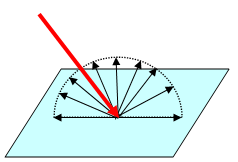
\includegraphics[width=0.4\linewidth]{images/chapter_stato_arte/stato_attuale_brdf_semistefa.png}\hfill
 \caption[BRDF superfici diffuse]{BRDF per superfici diffuse}
 \label{fig:stato_attuale_brdf_semistefa}
\end{figure}
Quindi la quantità di radiazione luminosa emessa della superficie (radianza) è proporzionale al flusso di radiazione luminosa incidente la superficie (irradianza) moltiplicato per il potere riflettente della superficie. 
\begin{equation}
L_s = \frac{r*E}{\pi}
\end{equation}
L’algoritmo prevede che ad ogni superficie ne corrisponda una analoga rappresentata da dei poligoni; non è necessario che ci sia una relazione 1:1 con i poligoni della superficie originale, infatti è possibile utilizzarne anche meno, o di più in caso si volesse un maggior dettaglio delle ombre.
\\
A questo punto viene creata una matrice di fattori forma con tutti i poligoni utilizzati. Questa matrice, dato un poligono i e un poligono j, restituisce il fattore forma Fij, ovvero un valore geometrico che denota una proporzione della quantità di luce che, partendo dal poligono i, arriva al poligono j.
\\
Una parte significativa dell’algoritmo radiosity è dedicata a calcolare in modo accurato i fattori forma tra tutti i poligoni della scena. 
Il fattore forma Fij dipende dai seguenti parametri:
\begin{itemize}
\item La forma dei due poligoni i e j.
\item L’orientamento dei due poligoni.
\item La distanza tra i e j.
\item L’occlusione di i e j a causa di altri poligoni.
\end{itemize}
Una volta ottenute tutte le relazioni geometriche tra i poligoni, alcuni poligoni sono designati come fonti luminose; questa designazione è necessaria per i processamenti al passo successivo.
\\
Come gia menzionato, le radiazioni luminose pervadono la scena fino ad ottenere una situazione di equilibrio; per calcolare questo equilibrio, l’algoritmo risolve un complesso sistema di equazioni lineari (riferimento bibliografico libro).
\\
Risolvendo questo sistema di equazioni lineari si ottengono i valori di radianza per ogni poligono, e quindi la radianza di tutta la superficie; questo avviene perchè la radianza nelle superfici diffuse è costante e non dipende dall’angolo di vista.
\\
La parte computazionalmente più onerosa è la risoluzione del sistema di equazioni lineari, e nonostante le GPU diventino sempre più veloci, il calcolo di alcuni algoritmi rimane tuttavia proibitivo per le applicazioni che necessitano di rendering real-time.
\\
Pertanto il calcolo dell’algoritmo radiosity viene fatto off-line, e le risultanti informazioni luminose possono essere memorizzate sui vertici delle superifici e poi interpolate, oppure memorizzate su delle lightmap per ogni superficie.
\\
In questo modo durante il ciclo di rendering, nella fase calcolo dello shading sui vertici delle geometrie, non sarà necessaria alcuna computazione delle informazioni di luce.
\newpage 
\begin{figure}[htb]
 \centering
 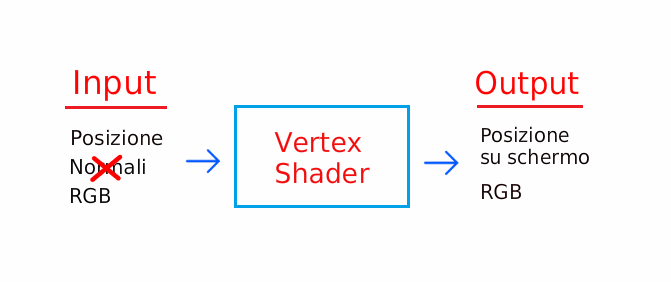
\includegraphics[width=0.8\linewidth]{images/chapter_stato_arte/stato_arte_ver_sh.jpg}\hfill
 \caption[Vertex shading lightmap]{Dettaglio circa l'operazioni di vertex shading utilizzando le lightmap.}
 \label{fig:stato_arte_ver_sh}
\end{figure}
La Id Software nel 1997 fu la prima software house che, per la realizzazione del videogioco Quake II, processò offline l’algoritmo radiosity, memorizzando le informazioni di luce su delle lightmap.
\\
\begin{figure}[htb]
 \centering
 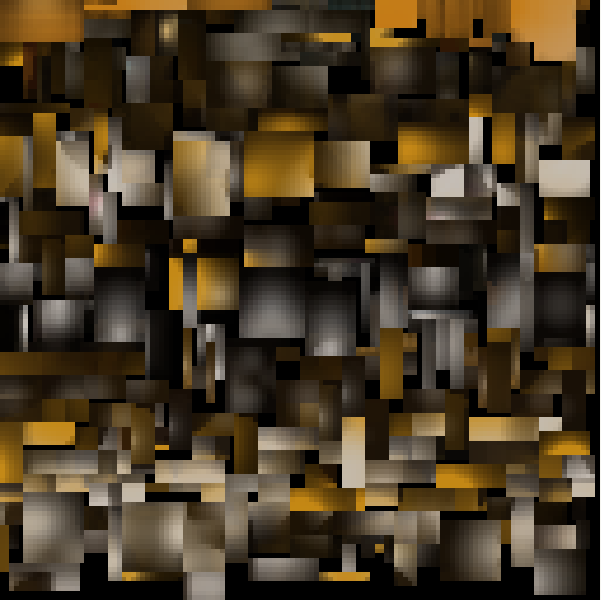
\includegraphics[width=0.4\linewidth]{images/chapter_stato_arte/stato_arte_quake_lightmap.png}\hfill
 \caption[Lightmap Quake II]{Una lightmap utilizzata nel videogioco Quake II (1997).}
 \label{fig:stato_arte_quake_lightmap}
\end{figure}
\\
Nonostante gli anni, il pre-calcolo offline delle luci rimane una tecnica attuale; ne è la prova The Witness, un gioco di avventura con elementi puzzle sviluppato da Thekla e uscito il 26 gennaio 2016. 
\\
Per lo stile grafico dell’opera l’autore Jonathan Blow vide l’illuminazione indiretta come soluzione migliore, in modo da poter simulare i rimbalzi di luce attraverso la scena ed ottenere un aspetto più ricco e delicato rispetto a soluzioni come quelle adottate generalmente dagli shooter in prima persona, dove si fa largo uso di illuminazione diretta, ombre dinamiche, ed effetti particellari. Siccome calcolare la luce indiretta in tempo reale sarebbe stato troppo gravoso, la soluzione finale fu quella di pre-computarla e mappare i risultati su delle   lightmap.	
\\
\begin{figure}[htb]
 \centering
 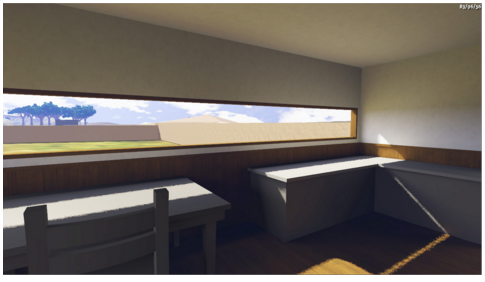
\includegraphics[width=0.8\linewidth]{images/chapter_stato_arte/stato_arte_lightmap_witness.png}\hfill
 \caption[Lightmap The Witness]{Un ambiente alpha con luci precomputate, tratto dal videogioco The Witness (2016)}
 \label{fig:stato_arte_lightmap_witness}
\end{figure}


\section{Environment map}
\label{sec:chapter_stato_arte_envmap}

Nella grafica computazionale, una environment map è un’efficiente tecnica utilizzata per approssimare la riflessione e rifrazione di oggetti tramite l’utilizzo di una texture precomputata.
La texture rappresenta l’ immagine dell’ ambiente che circonda uno o più oggetti nella scena.
L’ Environment map si basa principalmente su due assunzioni:
\begin{itemize}
\item L’ambiente è infinitamente distante dagli oggetti.
\item Gli oggetti non possono riflettere se stessi.
\end{itemize}
La prima assunzione permette di accedere alla environment map tramite la sola direzione in cui guarda l’osservatore. Il fatto che la env map non dipenda dalla sua posizione comporta però errori nella riflessione quando l’ambiente non è sufficientemente distante. 
\\
In tal caso è molto probabile che gli oggetti riflessi da un oggetto possano apparire in posizioni sbagliate.
\\
Questo errore è particolarmente riscontrabile su superfici in cui la riflessione dipende pesantemente dalla posizione (come gli specchi), mentre risulta quasi impercettibile su superfici curve. 
\\
Il presente aspetto verrà analizzato più nel dettaglio a fine paragrafo.
La seconda assunzione invece non permette di ottenere riflessioni multiple come ad esempio quelle ottenute da due oggetti vicini che si riflettono tra loro. Per questo motivo, è preferibile utilizzare l’environment map su oggetti convessi piuttosto che su oggetti concavi, i quali riflettono se stessi.
\\
Un oggetto viene detto convesso se comunque vengono presi due punti che gli appartengono anche il segmento che li congiunge gli appartiene interamente. In caso contrario l’ oggetto viene detto concavo. \cite{env1}
\begin{figure}[htb]
 \centering
 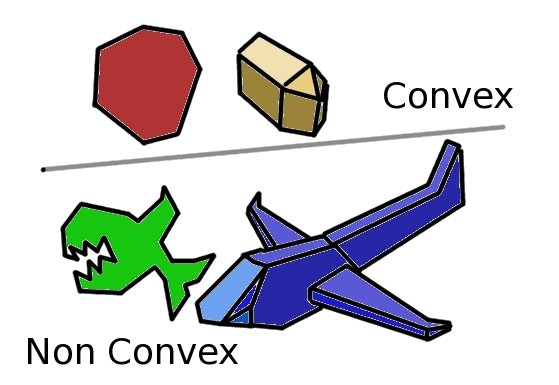
\includegraphics[width=0.5\linewidth]{images/chapter_stato_arte/stato_arte_conc_conv.jpg}\hfill
 \caption[Concavo,convesso]{Differenza tra oggetti convavi e convessi.}
 \label{fig:stato_arte_conc_conv}
\end{figure}
L’env map viene utilizzata ancora oggi nei videogiochi moderni permettendo di alleggerire notevolmente il carico computazionale del rendering real-time per la realizzazione di superfici riflettenti o rifrangenti.
\\
\begin{figure}[htb]
 \centering
 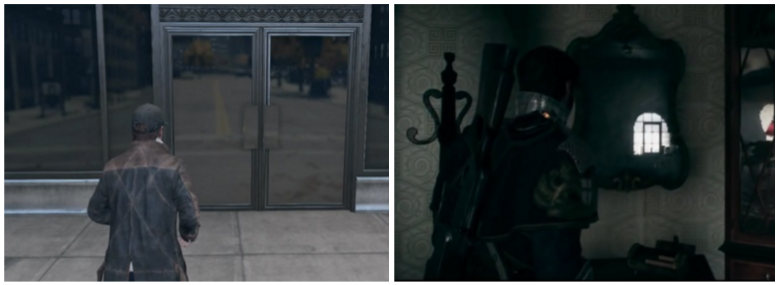
\includegraphics[width=1\linewidth]{images/chapter_stato_arte/stato_arte_wd_to.png}\hfill
 \caption[Le env map nei videogiochi]{Le env map sono tutt'oggi di ampio utilizzo in ambiente videoludico.}
 \label{fig:stato_arte_wd_to}
\end{figure}
\\
Videogiochi recenti quali Watch Dogs (a sinistra) e The Order: 1886 (a destra) ne fanno ampio utilizzo in quanto questa tecnica permette di ottenere un frame-rate costante anche in presenza di effetti complessi di riflessione e rifrazione. Siccome la texture utilizzata durante l’algoritmo di env-map è precomputata e rimane fissa, non è possibile però ottenere la riflessione/rifrazione dinamica di oggetti o personaggi in movimento (in entrambe le figure è possibile notare come  il personaggio in movimento non venga riflesso). Compromesso comunque accettabile in quanto il calcolo real-time di questi effetti potrebbe provocare una drastica diminuzione del frame-rate.
Nel presente lavoro di tesi l’utilizzo delle env-map ben si addiceva al contesto di lavoro preso in riferimento. Le scene di interni di appartamenti risultano infatti fisse nel tempo,  cosa che ha permesso di sfruttare questa tecnica per mantenere costanti le prestazioni dell’ applicazione anche in presenza di molti effetti di riflessione e rifrazione.

\subsection{L'algoritmo di environment-mapping}
\label{sec:chapter_stato_arte_algo_envmapping}

L’algoritmo di environment-mapping si comporta in maniera differente per superfici riflettenti e rifrangenti. Questo perchè le due superfici deviano in maniera differente i raggi che le colpiscono.
Le superfici riflettenti, riflettono il raggio di incidenza $i$ (partito dall’ occhio dell’ osservatore) che le colpisce in una direzione $r$ dipendente dalla normale $n$ sulla superficie.
\\
\begin{figure}[htb]
 \centering
 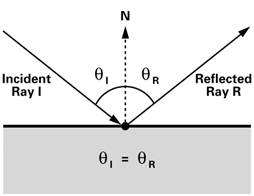
\includegraphics[width=0.5\linewidth]{images/chapter_stato_arte/stato_arte_inc_refl.png}\hfill
 \caption[Env map: riflessione]{Comportamento del raggio di incidenza i quando si ha un effetto di riflessione.}
 \label{fig:stato_arte_inc_refl}
\end{figure}

Per superfici perfettamente riflettenti (ad esempio uno specchio) l’angolo di incidenza $\Theta_i$ è lo stesso dell’ angolo di riflessione $\Theta_r$.
Il calcolo del vettore $r$ è essenziale per l’ algoritmo di env-map di riflessione ed il suo utilizzo verrà spiegato a breve durante la trattazione completa dei passi dell’algoritmo.
\begin{equation}
r = i - 2(n * i)n 
\end{equation}
Le superfici rifrangenti, invece, rifrangono  il raggio di incidenza $i$ che le colpisce in una direzione $t$ dipendente dal mezzo attraversato.
\\
\begin{figure}[htb]
 \centering
 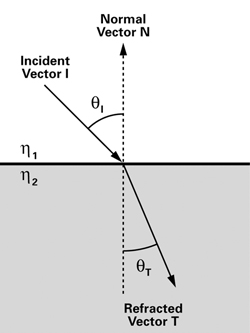
\includegraphics[width=0.4\linewidth]{images/chapter_stato_arte/stato_arte_refr.png}\hfill
 \caption[Env map: rifrazione]{Comportamento del raggio di incidenza i quando si ha un effetto di rifrazione.}
 \label{fig:stato_arte_refr}
\end{figure}
\\
La \emph{legge di Snell} \cite{env2} descrive la relazione tra l’ angolo di incidenza e di rifrazione di un raggio che transita tra due mezzi con indice di rifrazione differente.
\begin{equation}
n_1sin\Theta_1 = n_2sin\Theta_2 
\end{equation}
L’ equazione prevede quattro variabili: l’angolo di incidenza $\Theta_i$, l’angolo di rifrazione $\Theta_t$, l’indice di rifrazione del primo mezzo attraversato $n_1$ e l’indice di rifrazione del secondo mezzo attraversato $n_2$.
L’ indice di rifrazione è una grandezza adimensionale specifica per un mezzo che quantifica la diminuzione della velocità di propagazione della luce quando esso viene attraversato. Maggiore è l’indice di rifrazione per un mezzo, minore è la velocità di propagazione.
Nella figura l’indice di rifrazione $n_2$ è maggiore dell’ indice di rifrazione $n_1$. 
Siccome la velocità di propagazione è minore nel secondo mezzo rispetto al primo, anche l’angolo di rifrazione è minore rispetto all’angolo di incidenza (l’angolo è più vicino alla normale). 
L’equazione permette il calcolo del vettore $t$, essenziale per l’algoritmo di env-map di rifrazione:
\begin{equation}
t = \frac{\eta_1}{\eta_2}i + (\frac{\eta_1}{\eta_2}cos\Theta_i - \sqrt[2]{1 - sin^2\Theta_t})n
\end{equation}
Il calcolo del vettore $r$ e del vettore $t$ è semplice e questo rende l’environment map il metodo più veloce per renderizzare una superficie che rifrae o riflette.
L’ env-map prende il nome di \emph{env-map di riflessione} , quando viene utilizzata per simulare la riflessione e di \emph{env-map di rifrazione} quando viene utilizzata per simulare la rifrazione. Nulla vieta di utilizzare la stessa env-map per simulare entrambi gli effetti.
L’algoritmo usa il vettore $r$ quando viene utilizzata una env-map di riflessione e $t$ quando viene utilizzata una env-map di rifrazione.
Le operazione che l’ algoritmo effettua sono le seguenti: \cite{real_time_book}
\begin{itemize}
\item Generare o caricare una immagine a due dimensioni che rappresenta l’ ambiente ( l’env-map stessa).
\item Per ogni pixel che contiene un oggetto riflettente, calcolare la normale alla superficie dell’oggetto.
\item Computare il vettore $r$ oppure il vettore $t$.
\item Usare il vettore scelto come indice nella env-map per prelevare il valore che rappresenta la radianza entrante nella direzione di $r$ o $t$.
\item Usare il dato ottenuto dalla environment map come radianza. 
\end{itemize}
\begin{figure}[htb]
\centering
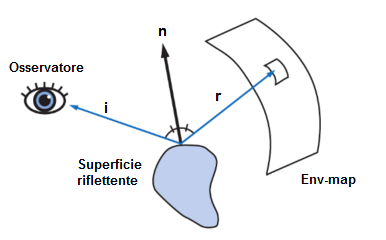
\includegraphics[width=0.6\linewidth]{images/chapter_stato_arte/stato_arte_env_alg.png}\hfill
\caption[Algoritmo environment mapping]{Environment mapping.}
\label{fig:stato_arte_env_alg}
\end{figure}
Il vettore r o t $(x,y,z)$, tramite una funzione di proiezione, viene convertito in un valore a due dimensioni $(u,v)$. Di fatto la env map viene utilizzata come una tabella a due dimensioni; il valore a due dimensioni viene utilizzato come indice e viene prelevato il valore di radianza del pixel da mostrare su schermo.
\\
Questo approccio produce risultati simili al ray tracing per quanto riguarda la riflessione o rifrazione, risultando però  più efficiente. 
Calcolare l’ angolo di incidenza e riflessione seguito da una ricerca nella env-map rispetto a calcolare l’esatta riflessione o rifrazione della luce tracciando un raggio e seguendo il suo percoso ottico semplifica di molto il lavoro eseguito dalla GPU. 

Esistono però problemi nell’ utilizzo della env map su superfici piatte in quanto i raggi che da esse vengono riflessi variano pochissimo in termini di angolazione. Questo si traduce in una proiezione delle componenti $(x,y,z)$ di $r$ o di $t$ in valori $(u,v)$ che sono molto simili per tutti i raggi riflessi dalla superficie. In questo modo i valori $(u,v)$ indicizzano solo una piccola porzione della tabella (env map) e questa porzione viene mappata su una superficie potenzialmente più larga. Il risultato visibile sulla superficie è quindi quello che solamente una piccola porzione della envmap viene riflessa sulla superficie e quest’ ultima può risultare ingrandita.
Inoltre nel caso di env map di rifrazione, l’algoritmo simula solo il primo raggio rifratto.
\\
\begin{figure}[htb]
\centering
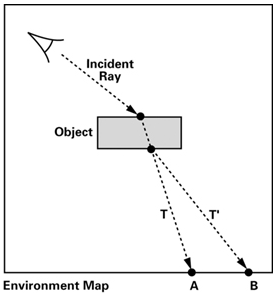
\includegraphics[width=0.5\linewidth]{images/chapter_stato_arte/stato_arte_refr_2.png}\hfill
\caption[Environment mapping: rifrazione]{Environment mappin: rifrazione}
\label{fig:stato_arte_refr_2}
\end{figure}
\newpage
Il raggio in realtà dovrebbe essere rifratto due volte: la prima quando entra nel mezzo, la seconda quando esce (vettore $T’$). Nella pratica però la seconda rifrazione non viene simulata ed il raggio prosegue nella direzione $T$ invece che in quella di $T’$. 
Questo tipo di semplificazione permette di alleggerire il carico di lavoro del render permettendo di ottenere una rifrazione convincente utilizzando un solo raggio.
Il risultato ottenuto da quest’ ultimo è sicuramente non accurato fisicamente come quello che si otterrebbe utilizzando due raggi ma comunque risulta molto simile.
Viene preferito questo approccio in quanto risulta più veloce e crea un credibile effetto di rifrazione.

\subsection{Env map cubica}
\label{sec:chapter_stato_arte_envmap_cubica}

Una env map cubica o cube map utilizza le immagini ottenute da sei facce di un cubo come env map \cite{env3} . 
L’ ambiente viene proiettato su ogni faccia del cubo e salvato tramite sei texture quadrate oppure disposte in sei diverse regioni di una singola texture (Fig. \ref{fig:stato_arte_cubo_envmap} ).
\begin{figure}[htb]
 \centering
 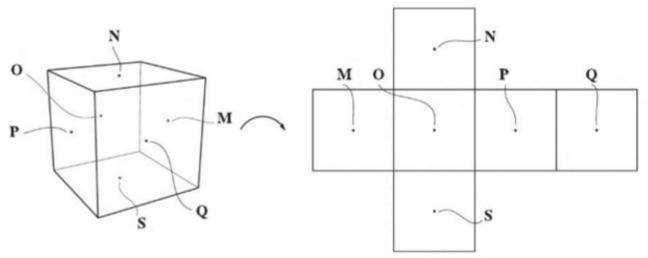
\includegraphics[width=0.6\linewidth]{images/chapter_stato_arte/stato_arte_cubo_envmap.png}\hfill
 \caption[Env map cubica]{Env map cubica}
 \label{fig:stato_arte_cubo_envmap}
\end{figure}
Nel dettaglio per ottenere una cube map, inizialmente viene piazzata una camera nella scena, successivamente viene proiettato l’ ambiente su ogni faccia di un cubo, disposto nel centro della camera, ed infine quest’ ultimo viene salvato su sei diverse texture quadrate o su una singola texture con sei diverse regioni cubiche (Fig. \ref{fig:stato_arte_texture_env_cubo} ).
\\
La scena viene quindi renderizzata sei volte (una per ogni faccia del cubo), con la camera posizionata al centro del cubo che guarda ad ogni faccia del cubo con un angolo di vista di 90 gradi.
\\
La forza di questo metodo è che l’ env map può essere facilmente generata real-time da qualsiasi renderer in quanto ha differenti vantaggi rispetto ad altre tecniche come le env-map sferica.
\\
L’ env map cubica, a differenza di quella sferica, è infatti indipendente dal punto di vista; infatti in applicazioni in cui il esso si muove non è necessario creare una nuova env-map per ogni nuovo punto di vista.
\begin{figure}[htb]
 \centering
 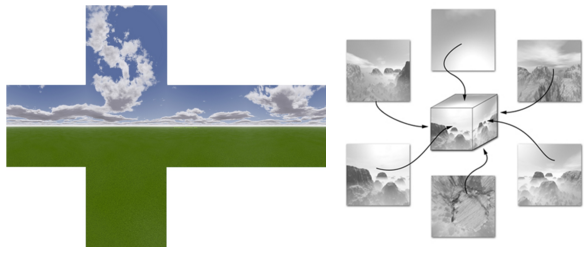
\includegraphics[width=0.9\linewidth]{images/chapter_stato_arte/stato_arte_texture_env_cubo.png}\hfill
 \caption[Env map texture]{Differenza tra una singola texture con sei regioni quadrate (sinistra), o sei texture quadrte distinte (destra).}
 \label{fig:stato_arte_texture_env_cubo}
\end{figure}

\section{Open GL}
\label{sec:chapter_stato_arte_open_gl}

OpenGL è una API, sviluppata dal Khronos Group nel 1992, per il controllo della GPU. L’obiettivo di OpenGL è quello di avere una API uniforme e multipiattaforma, indipendente dal linguaggio, che permette al programmatore di interfacciarsi con l’hardware di accelerazione grafica del sistema, senza occuparsi di come funziona l’hardware e il software sottostanti.
\\
Inoltre le sue funzionalità e comandi possono essere richiamati da ambienti di sviluppo basati su linguaggi molto differenti fra loro, quali Ada, C, C++, Fortran, Python, Perl e Java, fornendo inoltre una totale indipendenza dai protocolli e dalle tipologie di rete. 
Normalmente OpenGL viene fornito dai drivers della scheda video.
\\
L’API consiste in circa 150 comandi per la definizione di oggetti e per la creazione di applicazioni 3D interattive. Per essere indipendente dalla piattaforma, OpenGL non possiede alcun comando per realizzare operazioni su finestra, o per ricevere input dall’utente.
\\ 
A questo ci pensa il software con cui l’utente interagisce mediante GUI, il quale si occuperà di tradurre i comandi utente in direttive OpenGL per controllare l’hardware grafico sottostante. 
L’approccio di OpenGL con le strutture geometriche che si vogliono renderizzare è molto a basso livello; ogni modello è scomponibile in entità geometriche più semplici, dette primitive.
\\
Per primitive si intendono punti, linee, poligoni e immagini, ed ognuna di queste è generata considerando:
\begin{itemize}
\item La posizione rispetto le altre primitive.
\item I fattori di illuminazione rispetto le sorgenti di luce definite.
\item Il materiale che si intende simulare.
\item La texture applicata.
\item Il colore di ogni vertice, in base al quale cambierà il rendering del colore della texture.
\item Il valore di trasparenza.
\item Effetti aggiuntivi applicati alle primive, ad esempio tramite lo stencil-buffer. 
\end{itemize}
OpenGL ha enormi capacità di rendering: l’elevato numero di funzionalità di base offerte permette di scegliere tra moltissimi effetti e modalità di disegno, a tal punto che difficilmente si ha la necessità di implementarne di nuove.
\\
La grande varietà di cose che OpenGL permette di effettuare lo portano ad essere uno strumento piuttosto complesso da utilizzare, tuttavia la struttura base di un programma generico in OpenGL è piuttosto semplice: basta specificare gli oggetti da renderizzare, e inizializzare alcuni stati che servono a istruire OpenGL su come deve svolgere alcuni passi del rendering. 
\\
In effetti OpenGL è una vera e propria macchina a stati: utilizza infatti delle variabili di stato, le quali una volta settate, rimangono tali fino a nuova modifica. Tra i controlli impostabili mediante variabili di stato ci sono: modalità di disegno dei poligoni, posizione e caratteristiche delle luci, proprietà dei materiali degli oggetti da renderizzare.
\\
Alcune variabili di stato fanno riferimento a delle modalità che possono essere abilitate o disabilitate usando appositi comandi, come glEnable() o glDisable(). In generale ogni variabile ha un valore di default, e in qualsiasi momento è possibile interrogarle per sapere il valore attuale.
\\
Quando deve renderizzare oggetti, OpenGL viene coinvolto in una successione di fasi di processamento chiamata OpenGL rendering pipeline. L’obiettivo di questa pipeline è quello di ricevere primitive geometriche e di convertirle in pixel. La pipeline di render di OpenGL viene istruita su come deve elaborare le varie primitive mediante le variabili di stato sopra esposte.
I passi chiave della pipeline di rendering di OpenGL sono mostrati in figura \ref{fig:stato_arte_opengl_pipeline} , e per ognuno verrà fornita una descrizione generale del funzionamento:
\\
\begin{figure}[htb]
 \centering
 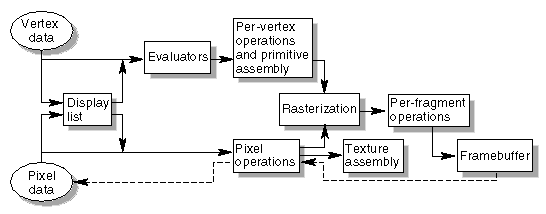
\includegraphics[width=0.9\linewidth]{images/chapter_stato_arte/stato_arte_opengl_pipeline.png}\hfill
 \caption[Pipeline di rendering di OpenGL]{Pipeline di rendering di OpenGL.}
 \label{fig:stato_arte_opengl_pipeline}
\end{figure}
\\
Tutti i dati, ad esempio delle descrizioni di geometrie, o delle descrizioni di pixel, vengono inizialmente memorizzati in una lista di elementi da renderizzare, detta \emph{display list}. Gia da questo punto è possibile istruire la pipeline affinchè, invece di memorizzare temporaneamente i dati in una lista, li processi immediatamente. 
\\
Una volta estratti i dati dalla lista inizia il processamento vero e proprio dei dati. La prima fase prevede che alla fine tutte le primitive geometriche siano descritte mediante vertici. Per ottenere ciò è necessario che tutte le primitive in input siano valutate in modo da individuare casi particolari come le curve parametriche, le quali sono descritte da punti di controllo e da funzioni polinomiali chiamate funzioni base. 
\\
In tal caso uno strumento di valutazione farà uso di un metodo di mappatura polinomiale per ottenere dai punti di controllo i vertici usati per rappresentare la superficie. Inoltre questo metodo consente di estrarre dai punti di controllo anche informazioni come normali di faccia, coordinate di texture e colore. 
\\
A questo punto le coordinate di ogni vertice vengono proiettate nel sistema di riferimento della camera mediante la matrice modello-vista. Inoltre, se abilitati, vengono calcolati gli effetti luminosi utilizzando i vertici proiettati, le normali  e le informazioni sul materiale e sulle luci; il risultato di questo calcolo sarà un colore.
\\
Il flusso di vertici viene interpretato in modo diverso a seconda di come è stata istruita la pipeline di rendering. Vi è infatti una informazione di connettività tra vertici che determina come i vertici devono essere connessi per creare una sequenza di primitive base. 
\\
Attraverso l’informazione di connettività dei vertici si può scegliere se le primitive base dovranno essere punti, linee, o poligoni. Ad esempio si supponga di avere una sequenza di sei vertici, e che l’informazione di connettività tra vertici indichi che il rendering deve utilizzare triangoli; l’interpretazione del flusso di sei vertici avrà come risultato due triangoli. 
L’output di questa fase è quindi composto da primitive geometriche base, insieme alle informazione sul colore, profondità, e altre informazioni utili alle fase di rasterizzazione.
\\
\begin{figure}[htb]
 \centering
 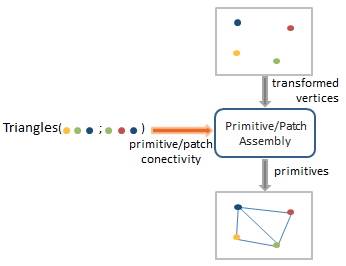
\includegraphics[width=0.5\linewidth]{images/chapter_stato_arte/stato_arte_prim_ass.png}\hfill
 \caption[Primitive Assembly]{Un'esempio di interpretazione delle primitive geometriche in base all'informazione di connettività fornita.}
 \label{fig:stato_arte_prim_ass}
\end{figure}
\\
Come visto nella prima fase della pipeline, la lista degli elementi da renderizzare può contenerei anche informazioni sui pixel, oltre che sulle geometrie. Mentre queste ultime sono soggette ai processamenti sopra descritti, i dati sui pixel vengono elaborati diversamente.
Per prima cosa i dati sono estratti dalla lista e copiati in una unità di memorizzazione governata da OpenGL in cui vige un determinato formato di immagine; di base esistono tre tipi di formato immagine:
\begin{itemize}
\item Colore: vengono memorizzati i colori in formato RGBA, ovvero ogni colore avrà una componente di rosso R, di verde G, e di blu B, e una componente alpha, usata solitamente dallo shader come valore di traslucenza, ma non solo. In generare viene sfruttata in modo diverso a seconda di come è stato istruito lo shader.
\item Profondità: questo formato memorizza le informazioni sulla profondità, necessarie  per i test di profondità sul depth buffer.
\item Profondità/Stencil: questo formato combina informazione di stencil e di profondità, e permette di allocare sia uno stencil buffer che un depth buffer.
\end{itemize}
La pipeline di rendering viene istruita in base al tipo di formato da adottare, influenzando così il modo in cui il dato deve essere interpretato.
Il trasferimento dei dati nella memoria di OpenGL è detto unpack.
Dopo lo spacchettamento dei dati, questi vengono scalati e processati mediante una mappa di pixel, e vengono ridimensionati in base al tipo di dato. Dopodichè vengono memorizzati in una area dedicata alle texture, per poi essere usati per la mappatura delle texture, o per essere dati in pasto al rasterizzatore. 
Per essere memorizzati in questa area, i dati sono prima raccolti in oggetti texture. Se nello stesso momento sono salvati troppi oggetti nella memoria texture, verranno mantenuti in memoria solo  gli oggetti texture ad alta priorità. 

A questo punto inizia il processo di rasterizzazione, in cui i dati sui pixel e quelli sulle geometrie, vengono convertiti in frammenti: partendo da una griglia di pixel in coordinate finestra, si individuano i pixel della griglia occupati dalle primitive. Successivamente ad ognuno di questi pixel si associa colore e profondità, ottenendo così un frammento. 
\\
\begin{figure}[htb]
 \centering
 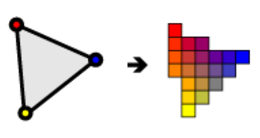
\includegraphics[width=0.4\linewidth]{images/chapter_stato_arte/stato_arte_raster.png}\hfill
 \caption[Rasterizzazione OpenGL]{Processo di rasterizzazione.}
 \label{fig:stato_arte_raster}
\end{figure}

Ogni frammento con coordinate di finestra $(x_w,y_w)$ prodotto dalla rasterizzazione, modificherà il pixel nel framebuffer che si trova nella stessa posizione in base a determinati parametri e condizioni. Questi sono valutati attraverso una serie di operazioni sui frammenti, mostrate in figura \ref{fig:stato_arte_frag_op}
\begin{figure}[htb]
 \centering
 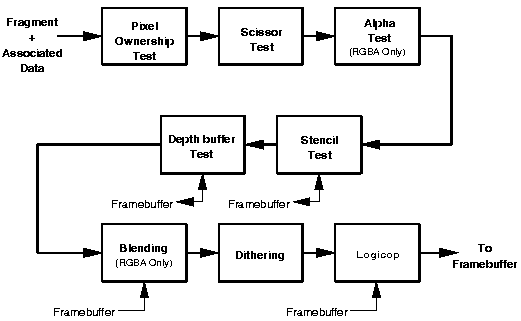
\includegraphics[width=0.9\linewidth]{images/chapter_stato_arte/stato_arte_frag_op.png}\hfill
 \caption[Operazioni sui frammenti]{Operazioni sui frammenti generati nella fase di rasterizzazione di OpenGL.}
 \label{fig:stato_arte_frag_op}
\end{figure}
\emph{Pixel ownership test} : si valuta se il pixel in posizione $(x_w,y_w)$ è presente nel framebuffer. Se non è presente, il frammento potrebbe essere scartato, oppure processato solamente da un sottoinsieme delle operazioni sui frammenti.
\\

\emph{Scissor test} : vengono scartati i frammenti al di fuori di una certa porzione rettangolare dello schermo definita mediante una funzione; questo test si può attivare o meno mediante \texttt{glEnable()} o \texttt{glDisable()} sulla variabile corrispondente allo stato di questo test. Se disattivato, il test avrà sempre esito positivo.
\\

\emph{Alpha test} : viene confrontato il valore alpha del frammento, con un valore di riferimento; il tipo di confronto $(>,\geq,<,\leq)$ dipende dalla costante scelta tra quelle offerte da OpenGL: never, always, equal, gequal, lequal, ecc.
\\

\emph{Stencil test} : viene confrontato i valore dello stencil buffer nella posizione $(x_w,y_w)$ del frammento con un valore di riferimento. Se il test ha esito negativo, il frammento viene scartato.
\\

\emph{Depth buffer test} : viene confrontato il valore del depth buffer nella posizione $(x_w,y_w)$ del frammento, con il valore $z_w$ del frammento stesso. Se il test non da esito positivo, il frammento viene scartato.
\\

\emph{Blending} : data la posizione $(x_w,y_w)$ del frammento, e la sua componente di colore RGBA, si prende la componente RGBA del pixel in posizione $(x_w,y_w)$ nel framebuffer, e la si combina con quella del frammento.
\\

\emph{Dithering} : Prima di spiegare questo processo è necessaria una premessa, ossia che per ogni pixel vengono memorizzate delle informazioni sui colori, e la quantità di informazioni memorizzata dipende dal numero di bitplanes che il sistema alloca al framebuffer.
Ad esempio se avessimo un 1 bitplane per l’informazione di colore di un pixel, per ogni pixel potremmo memorizzare l’informazione di colore in 1 bit; con 8 bitplanes avremmo 8 bit di informazione, e quindi 256 tonalità di colore possibili da memorizzare. 
\\
Ovviamente la quantità di bitplanes che un sistema alloca al framebuffer non può essere infinita, pertanto se si vuole aumentare la quantità di colori rappresentabili bisogna ricorre ad uno stratagemma; questo stratagemma è detto dithering, e a grandi linee il funzionamento è il seguente: supponiamo che la quantità di bitplanes allocata per le informazioni di colore non sia sufficiente a memorizzare il rosa, e supponiamo che un poligono necessiti questa colorazione. 
\\
Il dithering agisce in questo caso creando per l’occhio umano un illusione ottica, facendo apparire il poligono rosa quando in verità non lo è. Questa illusione è possibile coprendo l’area del poligono con un motivo “a scacchi”, dove ogni casella, ossia un pixel, assumerà una colorazione tra quelle disponibili nelle informazioni di colore, con l’obiettivo di ottenere come risultato complessivo, una tonalità di colore mancante nelle informazioni dei pixel. Ad esempio l’illusione del rosa è ottenibile alternando, in un motivo a scacchi, pixel rossi con pixel bianchi. Un tecnica simile al dithering è usata per rappresentare scale di grigi nelle foto dei quotidiani in bianco e nero.
\\

\emph{Logical operation}: L’ultimo passo corrisponde ad una serie di operazioni logiche tra colore e posizione del frammento, e colore e posizione del pixel nel framebuffer associato al frammento. Il risultati sostituiranno i valori del framebuffer nella posizione $(x_w,y_w)$ del frammento.
\\

Alcune implementazioni di OpenGL sono in grado di funzionare anche se il computer attraverso cui l’utente osserva il render di una scena è diverso dal computer che l’ha renderizzata.
Questa situazione è possibile se i computer sono connessi tra di loro mediante infrastruttura di rete.
\\
In un ambiente di questo tipo la macchina sulla quale è installato il software grafico, il quale traduce i comandi dell’utente in chiamate a funzioni di OpenGL, è detto client; questa è la macchina con cui l’utente sta interagendo. 
\\
La macchina che riceve le chiamate a funzione di OpenGL, e che processa la pipeline di render, è detta server. Il formato di interscambio di informazioni tra client e server è sempre lo stesso; in questo modo il programma OpenGL può funzionare in ambiente distribuito anche se le macchine comunicanti sono di diverso tipo. Se invece non è previsto che la specifica implementazione di OpenGL operi attraverso la rete, allora avremo un solo calcolatore che fungerà sia da client che da server.


In conclusions...



%\chapter{Tecnologie Abilitanti}
\label{cha:chapter_tecnologie_abilitanti}

Questo capitolo offre al lettore una descrizione esaustiva di tutte le tecnologie abilitanti per la realizzazione del sistema oggetto del presente elaborato di tesi. 
\\
Il sistema è composto da tre servizi principali per la costruzione, la resa fotorealistica, e la navigazione di scene 3D, il tutto su ambiente web.
\\
Per degli aspetti del sistema per cui esiste già una conoscenza pregressa, verranno utilizzate delle tecnologie già affermate; infatti se per un problema esiste già una soluzione comprovata, è inutile reimplementarla. 
\\
In particolare nel capitolo si parlerà di tecnologie per la gestione delle richieste utente, per abilitare la costruzione di ambient 3D sul browser, per il processamento del baking delle lightmap, e per la realizzazione di applicazioni web scalabili.

\section{Blender}
\label{sec:chapter_tecnologie_abilitanti_blender}

Blender è un software di computer grafica 3D professionale, gratuito ed open source. 
Viene utilizzato maggiormente per la creazione di film animati, effetti visivi, applicazioni 3D interattive e videogiochi.
Supporta interamente la pipeline 3D ed offre varie funzionalità avanzate come la modellazione 3D, la mappatura UV, l’ unwrap, la texturizzazione di oggetti, la simulazione di particelle, animazioni, rendering.
Il software dispone di un interprete interno Python grazie al quale offre delle API per la creazione ed esecuzione di script Python. 
Tali script permettono la realizzazione di applicazioni personalizzate in base ai propri interessi.
Python è un linguaggio di programmazione interpretato, interattivo ed orientato agli oggetti che comprende moduli, eccezioni, gestione dinamica dei tipi e classi. Inoltre le variabili non sono tipizzate e l’indentazione è necessaria per definire i blocchi.
Questa funzionalità di scripting è stata essenziale in questo lavoro di tesi per la creazione, tra le altre cose, di un tool che effettuasse il processo di baking in maniera automatica. Il tool verrà esaminato nei capitoli successivi.
Il software Blender è multi-piattaforma e compatibile con i sistemi operativi Linux, Windows e Macintosh.
\\
Attualmente il motore di default per il render è il Blender Render. Esso è un motore di tipo Biased in cui il calcolo della luce avviene secondo un’approssimazione visiva; viene calcolata la dimensione degli oggetti e la distanza delle luci, e da queste si ricavano ombre ed illuminazione.
Il punto di forza di questo tipo di motore è il totale controllo sulla luce ma può richiedere molta esperienza in campo fotografico ed artistico per poter essere padroneggiato. Ulteriore caratteristica positiva è l’efficienza; il motore permette di ottenere anteprime di rendering in minore tempo rispetto ad algoritmi di tipo Unbiased, come il path tracing.
Questo tipo di soluzione è però fisicamente non corretta in quanto non calcola i rimbalzi di luce sugli oggetti, non permettendo quindi di ottenere ombre e luci realistiche.
\\
Blender ha un ulteriore motore di render di tipo Unbiased chiamato Cycles, il quale permette di ottenere un’illuminazione fisicamente più corretta dei motori Biased.
Nel presente lavoro di tesi è stato scelto questo motore di rendering in quanto, a differenza del Blender Render, permette di ottenere sugli oggetti presenti nella scena degli effetti di luci ed ombre estremamente realistici; paragonabili a quelli nel mondo reale.
\begin{figure}[htb]
 \centering
 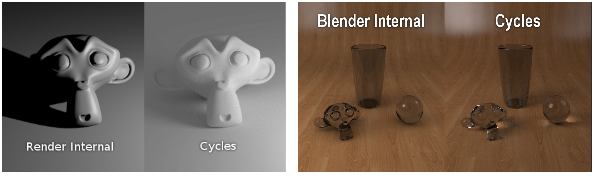
\includegraphics[width=0.9\linewidth]{images/chapter_tecnologie_abilitanti/tecnologie_abilitanti_bias_unbias.png}\hfill
 \caption[Cycles render e Blender render]{Confronto tra ombre e luci ottenute mediante Blender render (Unbiased) e Cycles render (Biased)}
 \label{fig:tecnologie_abilitanti_bias_unbias}
\end{figure}
Per modificare i materiali degli oggetti, le texture, ed il rendering in generale, Blender permette una metodologia di programmazione molto potente e flessibile, grazie al Node Editor. Tale strumento ha permesso di lavorare con il Cycles Renderer con estrema facilità ed è stato essenziale per permettere la creazioni di materiali complessi. 
\\
Maggiori dettagli circa il funzionamento del Node Editor verranno forniti nel capitolo [capitolo node editor].
\begin{figure}[htb]
 \centering
 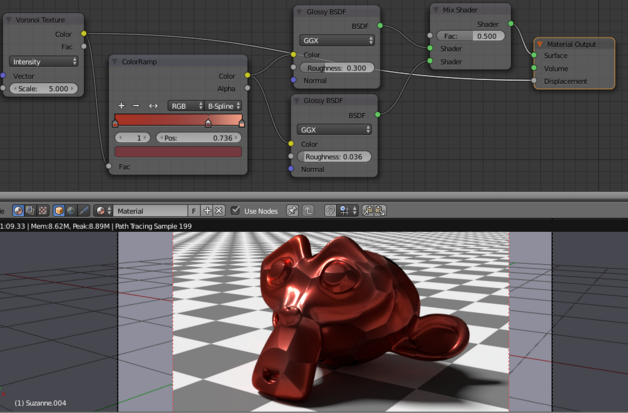
\includegraphics[width=1\linewidth]{images/chapter_tecnologie_abilitanti/tecnologie_abilitanti_node_editor.png}\hfill
 \caption[Blender Node Editor]{Il Node Editor di Blender}
 \label{fig:tecnologie_abilitanti_node_editor}
\end{figure}
Cycles correntemente supporta un integratore path tracing che funziona bene per la maggior parte degli effetti luce, ma non è cosi adatto per effetti caustici ed alcune complesse situazioni di luce. I raggi vengono lanciati dalla camera verso la scena, rimbalzando sulle superfici incontrate fino a quando viene raggiunta una fonte di luce come una lampada, un oggetto che emette luce, o lo sfondo della scena. 
Le luci vengono individuate sia tramite sample indiretto, in cui i raggi seguono il proprio percorso ottico fino a quando incontrano una fonte di luce, sia tramite sample di luce diretto, in cui si prende una luce e viene direzionato il raggio verso di essa.
\\
Per sample, come spiegato in precedenza, si intende il numero di raggi di luce che vengono tracciati per ogni pixel e Blender permette di indicare il numero di sample da utilizzare per effettuare il rendering della scena. Maggiore è il sample, migliore e meno rumoroso è il risultato ottenuto con il render.
\\
Nel dettaglio Blender utilizza due diversi integratori: l’integratore path tracer e l’integratore path tracer ramificato (\emph{branched path tracer}).
\\
L’integratore path tracer prevede un approccio classico, esaminato in dettaglio nel capitolo \ref{sec:chapter_stato_arte_ray_tracing}, in cui il raggio di luce ogni volta che colpisce un oggetto nella scena rimbalza in una direzione parzialmente casuale fino a quando non colpisce la fonte luminosa da cui riceve la luce.
Questo rende il singolo sample molto veloce da calcolare, ma ne richiede un numero elevato per ottenere un risultato di rendering pulito e senza rumore.
\begin{figure}[htb]
 \centering
 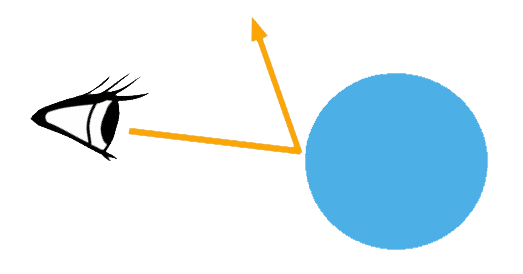
\includegraphics[width=0.6\linewidth]{images/chapter_tecnologie_abilitanti/tecnologie_abilitanti_sferaluce1.jpg}\hfill
 \caption[Integratore path tracer classico]{Integratore path tracer classico in cui il raggio di luce rimbalza in una sola direzione}
 \label{fig:tecnologie_abilitanti_sferaluce1}
\end{figure}
L’integratore path tracer ramificato (formalmente chiamato integratore non progressivo) prevede un approccio differente, in cui il raggio quando colpisce un oggetto  viene diviso in più raggi con direzioni randomiche. Sia la direzione che il numero di raggi in cui viene diviso sono dipendenti dal tipo di materiale di cui è costituito l’oggetto intersecato.
\\
Blender permette nel dettaglio di effettuare, tramite questo integratore, una più precisa parametrizzazione del sample voluto, permettendo di :
\begin{itemize}
\item Specificare il numero di sample da utilizzare, cioè il numero di raggi da lanciare, per ogni pixel del piano immagine tramite l’ attributo AA Render Samples.
\item Specificare un numero differente di sample o di raggi in cui il raggio viene diviso in base al tipo di materiale colpito, tramite gli attributi: \emph{Diffuse Samples}, \emph{Glossy Samples}, \emph{Transmission Samples}. Quindi se ad esempio il Diffuse Samples ha valore 5 mentre il Glossy Samples ha valore 2, il raggio viene diviso 5 volte quando colpisce un oggetto diffuse, mentre viene diviso 2 volte quando ne incontra uno glossy.
\end{itemize}
Questo permette di avere un maggiore controllo sul numero di raggi presenti nella scena e permette di creare configurazioni specifiche in base alla scena da renderizzare.
Se ad esempio in una scena fossero presenti molti oggetti con materiale glossy, ma pochi con materiale di tipo diffuse, il valore dell’attributo glossy samples può essere incrementato rispetto a quello diffuse, in modo da velocizzare il rendering degli oggetti diffuse che incidono poco sul risultato finale.
\\
Ogni sample quindi risulta più lento da calcolare rispetto l’approccio classico ma è richiesto un numero nettamente inferiore di sample per ottenere un risultato di rendering senza rumore.
Ad esempio in una scena in cui sono presenti solo oggetti con materiale diffuse, per ottenere un numero di sample equivalente all’ integratore path tracing classico, che ne utilizza 250, è necessario utilizzare 10 AA samples e 24 Diffuse Samples. Dove 10 x 25 = 250.
\begin{figure}[htb]
 \centering
 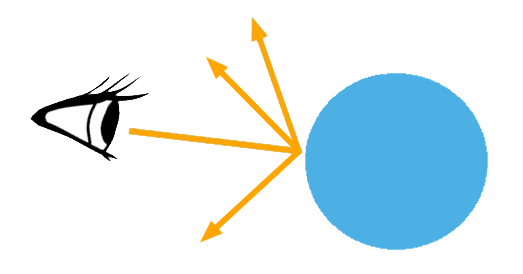
\includegraphics[width=0.6\linewidth]{images/chapter_tecnologie_abilitanti/tecnologie_abilitanti_sferaluce2.jpg}\hfill
 \caption[Integratore path tracer ramificato]{Integratore path tracer ramificato in cui il raggio di luce rimbalza in più direzione}
 \label{fig:tecnologie_abilitanti_sferaluce2}
\end{figure}
Per il presente lavoro di tesi è stato preferito utilizzare l’approccio di path tracing classico per facilitare all’ utilizzatore dell’ applicazione creata l’avvio di questo algoritmo. Egli infatti indicherà solamente un valore di sample senza dover necessariamente conoscere il funzionamento dell’ algoritmo. Algoritmo che avrebbe dovuto comprendere nel caso in cui avesse utilizzato l’approccio ramificato.
Oltre al samples esistono ulteriori parametri per effettuare il rendering ma questi verrano analizzati nel dettaglio nei capitoli successivi.
\\
Infine Blender offre il rendering GPU permettendo di utilizzare la scheda grafica, al posto della CPU, per migliorare notevolmente i tempi di rendering grazie alla maggiore potenza di calcolo.
In particolare Cycles prevede due modalità di rendering GPU:
\begin{itemize}
\item CUDA: l'architettura di elaborazione in parallelo che permette il rendering veloce su schede grafiche NVidia.
\item OpenCL: supporta il rendering su schede grafiche AMD/ATI, però ancora in fase sperimentale.
\end{itemize}
In questo lavoro di tesi è stato utilizzato CUDA per ottenere miglioramenti netti nei tempi di rendering permettendo di velocizzare notevolmente il servizio creato.

\section{Node JS}
\label{sec:chapter_tecnologie_abilitanti_nodejs}

Node.js è un framework open-source, multi-piattaforma che permette lo sviluppo di applicazioni web lato server scritte in JavaScript ed eseguibili su Linux, Microsoft Windows ed OS X.
La piattaforma è costruita sull’ engine Javascript runtime V8 di Google, utilizzato anche da Chrome/Chromium.
\\
Node.js nasce con l’ obiettivo di facilitare la realizzazione di applicazioni web lato server, contenendo a tal proposito librerie integrate per la creazione di web-server altamente scalabili.
Esso non sfrutta il classico modello basato su processi o thread concorrenti ma prevede una architettura basata su singolo thread ed una API di I/O non bloccante, fondamentale per la creazione di applicazioni web real-time altamente produttive e scalabili.
\\
Nello specifico lo sviluppatore utilizza un modello asincrono di programmazione basato su eventi in cui vengono eseguite azioni solo al verificarsi di uno specifico evento. 
Quando ad esempio viene richiesto un valore ad un server remoto, l’istruzione che ha effettuato la richiesta non blocca l’esecuzione ma viene saltata.
\\
In questo modo l’esecuzione è in grado di proseguire con le istruzioni successive senza dover attendere il valore richiesto.
\\
La funzione di callback viene eseguita solamente quando è completata la chiamata remota ed il controllo dell’ esecuzione è tornato all’istruzione sospesa.
Questo metodo garantisce un’ ottimizzazione delle performance quando si lavora su web. 
I tempi di attesa tra una richiesta HTTP e l’ altra risulterebbero, infatti, troppo lunghi rispetto ai tempi di lavoro del processore e quindi attendere una risposta rallenterebbe troppo il sistema.
\\
Ogni funzione in Node.js è asincrona, quindi le istruzioni che normalmente bloccherebbero il thread vengono invece eseguite in background.
\\
\begin{figure}[htb]
 \centering
 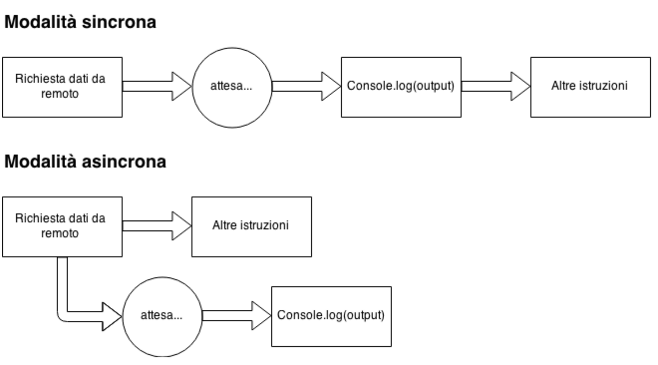
\includegraphics[width=0.9\linewidth]{images/chapter_tecnologie_abilitanti/tecnologie_abilitanti_node_mod.png}\hfill
 \caption[NodeJS: modalità sincrona e asincrona]{Differenza tra modalità sincrona e asincrona}
 \label{fig:tecnologie_abilitanti_node_mod}
\end{figure}
\\
Ad esempio per leggere un file in maniera asincrona bisogna specificare una funzione di callback da eseguire una volta che l’ operazione di lettura è stata completata.
La callback è una funzione che viene chiamata solo dopo che un dato task è stato completato.
Un esempio di callback è il seguente :
\begin{lstlisting}[language=javascript]
var callback = function(err, contents) {
	console.log(contents);
}
fs.readFile('etc/hosts', callback);
console.log('Fai qualcos\'altro...');
\end{lstlisting}
Il codice è non-bloccante in quanto la funzione che esegue la lettura inizia a leggere il file e ritorna immediatamente il controllo all’ambiente di esecuzione, permettendo l’esecuzione delle istruzioni successive( stampa a video di una stringa nell’esempio). 
La callback viene invocata solamente quanto il file è stato letto.
\\
Quindi le callback rappresentano un approccio comodo e molto utilizzato soprattutto nelle interazioni con il server; tuttavia il loro utilizzo in situazioni complesse può presentare problemi.
\\
Quando ad esempio viene sottomessa ad un server una richiesta per l’elenco dei post e delle foto pubblicati sul blog di un utente, vengono effettuate tre chiamate al metodo \texttt{get()}. 
Ciascuna \texttt{get()} ha la relativa funzione di callback (passata come terzo argomento), che viene eseguita quando il server restituisce il risultato richiesto.
\begin{lstlisting}
$.get("/users", {id: "12345"},
 function(user) {
  $.get("/blogs", {id: user.blogId},
   function(blog) {
   	displayPostList(blog.posts);
   });
  $.get("/photos", {id: user.albumId},
   function(album) {
   	displayPhotoList(album.photos);
   }
  );	
 }
);
\end{lstlisting}
La prima callback viene invocata quando la prima get restituisce la rappresentazione json dell’ utente richiesto. Le altre 2 get sono annidate dentro la prima callback in quanto dipendenti dall’esito della prima chiamata.
\\ 
Visto che la visualizzazione dei post e delle foto è asincrona, non necessariamente quest’ultime verranno visualizzate dopo i post. Quindi per vincolare l’ordine di visualizzazione o per effettuare ulteriori elaborazioni su entrambi gli insiemi di risultati prima di visualizzarli (come mostrare solo le foto relative ai post), bisogna trovare un modo per sincronizzare le callback; cosa tutt’altro che semplice.
\\
Da questo esempio quindi è possibile notare i principali difetti derivanti da un uso intensivo delle callback:
\begin{itemize}
\item Scarsa leggibilità del codice, che tende facilmente a svilupparsi verso destra a causa dei molteplici annidamenti delle callback.
\item Difficoltà di composizione delle callback e di sincronizzazione del flusso di elaborazione.
\item Difficoltà nella gestione degli errori e nel debug, soprattutto in presenza di callback anonime. Non è possibile infatti gestire l’eccezione all’interno della funzione chiamante la callback.
\end{itemize}
Il problema principale è che dall’ esecuzione di chiamate asincrone, diversamente da quelle sincrone, non si ottiene un valore di ritorno o una eccezione. Non è possibile quindi la composizione di funzioni e la gestione di eventuali eccezioni.
Per questo motivo l’api di node, che prima faceva solamente uso delle callback, permette ora anche l’utilizzo delle promesse.
\\
Le promesse, o promise, sono oggetti che rappresentano il risultato di una chiamata di funzione asincrona. L’ oggetto, nel dettaglio, rappresenta la promessa che un risultato verrà fornito non appena disponibile.
Il vantaggio principale nell’utilizzo delle promesse rispetto alle callback consiste nel rendere il codice più leggibile in quanto più simile al flusso di esecuzione sincrono.
La componente principale dell’oggetto promessa è il suo metodo then. 
Il metodo then viene invocato una volta ottenuto il risultato dell’ operazione asincrona e prende come argomento due callback opzionali, una eseguita quando l’operazione è andata a buon fine, l’altra in caso di errore.
\begin{lstlisting}[language=javascript]
var promise = doSomethingAsync();
promise.then(onFulfilled, onRejected);
\end{lstlisting}
Il conclusione quindi il fatto che Node.js operi su thread singolo ed utilizzi chiamate I/O non bloccanti, piuttosto che usare thread concorrenti, permette il supporto di decine di migliaia di connessioni senza pagare il costo dovuto al cambiamento di contesto; risultando quindi ideale per applicazioni real-time altamente concorrenti, applicazioni I/O bound, applicazioni data streaming. 
\\
Operare con un singolo thread però non consente la scalatura orizzontale; non comporta quindi benefici in termini di prestazioni all’ aumentare numero di processori fisici. 
Per questo motivo non è consigliabile utilizzare Node.js per applicazioni che fanno utilizzo intensivo della CPU.
Nel presente lavoro di tesi Node.js ha permesso la creazione di un server in grado di accettare richieste concorrenti da parte dei client, i dettagli verrano esaminati nei capitoli successivi.



\section{Web component e Polymer}
\label{sec:chapter_tecnologie_abilitanti_webcomp_poly}

Al giorno d’oggi le applicazioni web sono molto complesse: è fondamentale trovare il modo corretto di suddividere lo sviluppo dell’applicazione in più componenti non sovrapposte, in modo che il team di sviluppo operi in maniera più efficiente. 
Ogni componente del sistema deve garantire la proprietà di isolamento, per nascondere la propria complessità agli altri componenti.
Un buon isolamento tra componenti rende il software più manutenibile e semplice da sviluppare.
Inizialmente la complessità delle applicazioni web veniva gestita lato server, isolando l’applicazione in più pagine web; questo obbligava l’utente a dover navigare molte pagine sul browser.
Con l’avvento di tecniche come AJAX, che hanno semplificato la realizzazione di single page applications, gli utenti hanno cominciato a fruire di una esperienza d’uso più fluida, simile a quella che si ha con le applicazioni desktop. 
La logica delle applicazione lato client, che spesso è anche più complessa di quella lato server, può essere isolata all’interno di una singola pagina web o documento mediante i web component.

I web component sono un’ insieme di tecnologie prodotte da  Google e approvate dal W3C che consentono la creazione di widget, ovvero elementi html che includono logica di funzionamento e stile, che possono essere importate in documenti o applicazioni web. Da una widget viene separata ogni responsabilità che ha a che fare con altre widget; di conseguenza ogni elemento non dipende dai dettagli implementativi degli altri elementi. Sono possibili dipendenze solo tra le interfacce esposte dalle widget. 
Assegnare le responsabilità in questo modo permette al modello a componenti di soddisfare la proprietà di incapsulamento.
Inoltre la fruibilità di elementi html facilmente integrabili nell’applicazione permette alle componenti di interagire in modo semplice tra loro; in questo modo è soddisfatta anche la proprietà di interoperabilità tra componenti.
Questi web component sono parte del browser, quindi non hanno bisogno di librerie esterne per essere usati, ma basta includerli aggiungendo un tag nella pagina html. 
Una widget è portabile e gode di un elevata riusabilità; inoltre all’interno di una widget è possibile effettuare tutto ciò che è consentito dai linguaggi html, css e JavaScript. 
L’obiettivo principale dei web component è cambiare il modo in cui le applicazioni web vengono create, consentendo agli sviluppatori di estendere il vocabolario HTML creando nuovi elementi HTML riusabili. Questa aggiunta permette agli sviluppatori di interfacciarsi a più alto livello con lo sviluppo di applicazioni web, definibili mediante aggregazione di più componenti.
Quando si parla di web components in verità si parla di quattro tecnologie differenti, le quali insieme forniscono tutti gli strumenti necessari per creare i propri componenti.
Tali tecnologie sono: Custom Elements, Templates, HTML Imports e Shadow DOM. 

\subsection{Custom elements}
\label{sec:chapter_tecnologie_abilitanti_custom_elements}

La tecnologia custom element permette di creare nuovi elementi HTML all’interno del DOM del browser; ogni elemento racchiude logica di funzionamento, stile CSS e un tag HTML necessario per importare l’elemento nelle applicazioni web. 
Nonostante questi elementi facciano parte dei web components, possono essere utilizzati anche come entità separate. Uno dei motivi per cui è stata creata la tecnologia Custom Elements è la possibilità di introdurre le lifecycle callbacks, che consentono di associare specifici comportamenti ad un elemento HTML durante il suo ciclo di vita. Ad esempio è possibile istruire un elemento HTML sul comportamento che deve assumere nel momento in cui viene inserito nel DOM, e su quello che deve assumere quando viene rimosso dal DOM. 
Per registrare un nuovo elemento HTML nel browser si usa il metodo \texttt{Document.registerElement()}, e il nuovo elemento utilizzerà di default l’interfaccia HTMLElement; se invece l’elemento non viene registrato sul browser, userà l’interfaccia HTMLUnknownElement. E’ anche possibile creare un elemento HTML come estensione di un elemento nativo, come \texttt{<button>}; in questo caso però non sarà possibile includere l’estensione nel DOM come elemento a se stante, ma sempre insieme all’elemento nativo che estende; ad esempio l’inclusione sarà \texttt{<button is=”my button”>} e non \texttt{<my-button>} .
I vantaggi apportati dalla tecnologia custom elements sono:
\begin{enumerate}
\item Definizione e creazione di nuovi elementi HTML/DOM.
\item Estendere la logica funzionale di elementi nativi mediante nuovi elementi.
\item Racchiudere tutte le funzionalità di un nuovo elemento in un tag.
\item Estendere le API degli elementi del DOM nativi.
\item Estrema utilità nelle Single Page Applications.
\end{enumerate}
A questo punto verrà mostrato come è possibile creare un nuovo custom element utilizzando ad esempio le classi di JavaScript 6.
Per prima cosa viene definita la classe, la cui struttura è tipicamente la seguente:
\begin{lstlisting}[language=JavaScript]
class MyButton extends HTMLElement {    
/* E possibile estendere 
   qualsiasi altro elemento o classe */
/* Costruisco le proprieta dell'elemento 
   esteso, ovvero HTMLElement */     
   constructor() {          
      super();                         
   }   								  
/* Qui vengono definite quelle necessarie 
   tra le quattro lifecycle callbacks offerte:
   createdCallback(){ . . } 
   attachedCallback(){ . . } 
   detachedCallback(){ . . } 
   attributeChangedCallback() { . . } */
/* Qui vengono definiti i metodi getters e setters:
   set ...{ . . } 
   get ...{ . . } */
}
\end{lstlisting}
Come discusso in precedenza, le lifecycle callback risultano uno strumento utile nella definizione di un custom element, Lo sviluppatore può decidere di implementare una delle quatto callback disponibili:
\begin{itemize}
\item \emph {createdCallback} - Il comportamento dell’elemento quando viene registrato.
\item \emph {attachedCallback} - Il comportamento dell’elemento quando viene inserito nel DOM.
\item \emph {detachedCallback} - Il comportamento dell’elemento quando viene rimosso dal DOM.
\item \emph {attributeChangedCallback(attributeName)} - il comportamento dell’elemento quando un suo attributo viene modificato.
\end{itemize}
\emph{createdCallback} viene invocata in modo sincrono alla creazione dell’elemento, le altre callback sono invece chiamate in modo asincrono. Le callback asincrone solitamente sfruttano \texttt{MutationObserver} per mettersi in ascolto dei cambiamenti sul DOM; questo consente alle callbacks di essere invocate prima di altri elementi come layout, stile, o altri eventi; in questo modo si evitano problemi, come il caricamento di contenuto senza stile, prima che la callbacks abbiano modo di reagire alle modifiche sul DOM.
Per la definizione di metodi o proprietà, possono essere utilizzati dei metodi getter e setter:
\begin{lstlisting}[language=JavaScript]
set properties(prop) {
     this.mybutton_text = prop.text;
}

get text() {
     return this.textContent;
}
\end{lstlisting}
Una volta definite le callback e i getter e setter è possibile attivare il nuovo elemento, utilizzando il metodo \texttt{Document.registerElement()}:
\begin{lstlisting}[language=JavaScript]
var mybutton = document.registerElement("my-button", MyButton);
\end{lstlisting}
A questo punto il nuovo elemento si può includere nel documento HTML, usando direttamente i tag:
\begin{lstlisting}[language=HTML5]
<my-button></my-button>
\end{lstlisting}
oppure in Javascript:
\begin{lstlisting}[language=JavaScript]
var custom_button = new MyButton
document.getElementById("something").appendChild(custom_button)
\end{lstlisting}
E’ possibile associare uno stile al nuovo elemento in due modi:
Specificandolo nell’implementazione della lifecycle callback \emph{createCallback} :
\begin{lstlisting}[language=JavaScript]
createdCallback(){ 
     this.innerHTML = ""+ 
         " <style> "+ " p { color: orange; } "+ " </style> "+ 
         .
         .
         + "";
}
\end{lstlisting}
Oppure utilizzando un file css standard:
\begin{lstlisting}[language=HTML5]
my-button > p { 
background-color:#FFA500;
}
\end{lstlisting}

\subsection{HTML imports}
\label{sec:chapter_tecnologie_abilitanti_html_imports}

HTML imports è un modo per importare e riusare documenti HTML in altri documenti HTML. Come il tag \texttt{<script>} permette di iniettare codice Javascript nelle pagine, così HTML imports permettere di iniettare intere risorse HTML. In particolare HTML imports permette di importare dei custom element da URL esterni. In generale si può dire che HTML imports è il meccanismo di pacchettizzazione per le tecnologie Web Components.
Per importare una risorsa HTML si inserisce nel documento il tag \texttt{<link>} come mostrato dall’esempio:
\begin{lstlisting}[language=HTML5]
<link rel="import" href="myfile.html">
\end{lstlisting}
L’elemento HTML \texttt{<template>} è un meccanismo per mantenere nel DOM un contenuto HTML lato client che non viene renderizzato quando la pagina viene caricata, ma che può essere successivamente istanziato a tempo di esecuzione usando JavaScript. Un template può essere visto come un frammento di contenuto che viene memorizzato per un successivo uso all’interno del documento. Durante il caricamento della pagina il parser del browser processerà comunque il contenuto del \texttt{<template>} , ma solo per assicurarsi che il contenuto sia valido, dopodichè tale contenuto non verrà renderizzato.
Per creare un elemento \texttt{<template>} , basta definire il template content e racchiuderlo tra i tag \texttt{<template>} :
\begin{lstlisting}[language=HTML5]
<template id="mytemplate">
  <img src="" alt="great image">
  <div class="comment"></div>
</template>
\end{lstlisting}
Se incluso in un elemento template, un contenuto HTML gode delle seguenti proprietà: 
\begin{itemize}
\item Il contenuto è inattivo e nascosto finchè non viene attivato esplicitamente.
\item Il contenuto inattivo non ha alcun effetto collaterale: non verrà eseguito alcuno script, non verrà caricata nessuna immagine, o eseguiti file audio.
\item Il contenuto inattivo è come se non fosse presente nel documento: usando \texttt{document.getElementById()} o \texttt{querySelector()} nella pagina principale non verrà restituito alcun nodo figlio di un \texttt{<template>}
\item Il template può essere posizionato ovunque all’interno di \texttt{<head>}, \texttt{<body>}, o \texttt{<frameset>}, e può includere qualsiasi tipo di contenuto ammissibile nei tre tag sopra citati. Può essere posizionato anche come figlio di una \texttt{<table>} o di una \texttt{<select>}. 
\end{itemize}
Per utilizzare un template bisogna attivarlo. Il modo più semplice per farlo è creare un clone della proprietà .content del template mediante \texttt{document.importNode()}. la proprietà \texttt{.content} è un \texttt{DocumentFragment} di sola lettura, contenente il template content. Una volta appeso al DOM, il clone si attiva.
\begin{lstlisting}[language=JavaScript]
var t = document.querySelector('#mytemplate');
var clone = document.importNode(t.content, true);
document.body.appendChild(clone);
\end{lstlisting}

\subsection{Shadow DOM}
\label{sec:chapter_tecnologie_abilitanti_shadow_dom}

Shadow DOM è la tecnologia core dei Web Components. Shadow DOM permette di incapsulare le implementazioni degli elementi in un albero DOM separato, in modo da separarle dal resto del documento, e allo stesso tempo proteggere il documento dai cambiamenti introdotti dal componente. Uno dei motivi per cui viene utilizzato lo shadow DOM è lo stile; lo stile di un web component non dovrebbe influenzare lo stile della pagina che lo ospita, e viceversa la pagina ospitante non dovrebbe influenzare lo stile del componente; questa situazione può manifestarsi ad esempio nei grandi siti, dove spesso il css è male organizzato. In generale lo Shadow DOM fornisce ad un normale albero DOM il supporto adeguato all’incapsulamento sia per JavaScript che per CSS; inoltre fornisce lo strumento necessario a controllare come diversi alberi DOM interagiscono l’uno con l’altro. 
Lo shadow DOM è rappresentato dalla propria radice, detta \emph{shadow root}.
Un elemento in cui è inserito un nodo shadow root è detto \emph{shadow host}. Il contenuto di uno shadow host viene renderizzato, mentre quello dello shadow root no. 
Nella tecnologia shadow DOM un nodo può esprimere tre diversi tipi di alberi: \emph{light DOM}, \emph{shadow DOM} e \emph{composed DOM}.
Al Light DOM e allo shadow DOM si può anche fare riferimento con il nome logical DOM; questo è il DOM con cui lo sviluppatore interagisce. Il composed DOM è ciò che il browser vede, e che usa per renderizzare i pixel su schermo.

Il light DOM di un custom element viene visto dall’utente finale come un normale sottoalbero. Quindi può accedervi per chiedere informazioni usando \texttt{.childNodes}, \texttt{.children}, \texttt{.innerHTML} o qualsiasi altro metodo o proprietà di un comune sottoalbero.
\begin{lstlisting}[language=HTML5]
<custom-element>
  <p>something hidden from end user</p>
  <h1>Hello World</h1>
</custom-element>
\end{lstlisting}
Un elemento custom può definire uno shadow DOM associando un nodo shadow root a se stesso. Lo shadow DOM è interno all’elemento e celato all’utente finale. I suoi nodi non sono figli del custom element. Un nodo shadow root viene definito in questo modo:
\begin{lstlisting}[language=HTML5]
#shadow-root
  <!-- tutto cio che viene definito qui dentro andra
  	   nello shadow DOM del custom element -->
  <p>something hidden from end user</p>
\end{lstlisting}
E un tipico utilizzo per associarne uno ad un custom element:
\begin{lstlisting}[language=JavaScript]
var cel = document.getElementById('custom-element');
var shadow = cel.createShadowRoot();
document.body.appendChild(cel);
\end{lstlisting}
Il composed DOM è ciò che il browser renderizza. Per il rendering, il light DOM viene distribuito nello shadow DOM per creare il composed DOM; nel nostro esempio il composed DOM avrà questo aspetto:
\begin{lstlisting}[language=HTML5,label={custom_el_code}]
<custom-element>
  <p>something hidden from end user</p>
  <h1>Hello World</h1>
</custom-element>
\end{lstlisting}
I nodi nel light DOM o nello shadow DOM esprimono relazioni tra parenti o fratelli che corrispondono a quelle dei rispettivi alberi a cui appartengono; le relazioni che esistono nel composed DOM finale non sono espresse da nessuna parte nel DOM. Guardando l’esempio \ref{custom_el_code} questo vuol dire che, anche se dal composed DOM si evince che \texttt{<p>}, così come \texttt{<h1>}, sono figli di \texttt{<custom-element>}, in verità il primo è figlio dello shadow DOM, mentre il secondo è figlio del light DOM. I due nodi non solo relazionati, ma il composed DOM li renderizza come se lo fossero. In questo modo l’utente può manipolare light e shadow DOM come se fossero normali sottoalberi del DOM, lasciando poi al sistema l’onere di sincronizzare i due nell’albero di render finale.

I produttori di browser sono tutt’oggi al lavoro per introdurre nativamente il supporto ai web components:
\begin{itemize}
\item \textbf{Google Chrome} è al momento il punto di riferimento per il supporto ai Web Components, principalmente per il fatto che Google è uno dei principali promotori di questi nuovi standards. Tutti e quattro di standards dei Web Component hanno un supporto nativo in Chrome e possono essere usati senza bisogno di polyfills. 
\item \textbf{Firefox} utilizza un’implementazione di Templated e offre la possibilità di attivare Shadow DOM e i Custom Elements. Al momento l’implementazione di HTML Imports è in standby in quanto si temono eccessive sovrapposizioni con ECMAScript 6 (ES6), ovvero lo standard su cui si basa l’implementazione JavaScript di SpiderMonkey, l’engine utilizzato da Mozilla. 
\item \textbf{Safari} ha un supporto per Templates e recentemente ha aggiunto un supporto per Shadow DOM. Esiste anche un prototipo di implementazione di Custom Elements, ma come per Mozilla, il team di WebKit, il motore su cui si basa Safari, pensa che i moduli ES6 debbano essere la base per l’import di nuovi elementi custom e quindi non sta lavorando attivamente ad un supporto per la tecnologia.
\item \textbf{Microsoft} ha da poco aggiunto un supporto per HTML Template in Edge 13. l’obiettivo è quello di fornire al browser un supporto completo ai Web Components.
\end{itemize}

Siccome nella stragrande maggioranza dei browser ancora non è presente un supporto nativo ai Web Components, molti fanno ancora affidamento al \emph{Web Components Polyfill}.
Per polyfill si intende una porzione di codice, comunemente detta plugin, che permette di introdurre nel browser una tecnologia che nativamente non offrirebbe. 
Grazie al polyfill, molti browsers, tra cui Internet Explorer 11, hanno il supporto ai Web Components. 
Un browser con supporto nativo ai Web Components può garantire prestazioni d’uso migliori. Il Web Components Polyfill usato dai browser per includere il supporto ai Web Component si chiama \texttt{Webcomponent.js}

\texttt{Webcomponents.js} è un insieme di polyfills che implementano le tecnologie dei Web Components. Grazie a questo plugin gli sviluppatori possono usufruire dei Web Component su tutti i browsers moderni, ad eccezione di Google Chrome, che non necessita più dello strato polyfill.



\section{WebGL}
\label{sec:chapter_tecnologie_abilitanti_webgl}
WebGL (Web Graphics Library) è una API Javascript che permette il rendering interattivo su browser web senza il bisogno di installare plug-in aggiuntivi.
Esso è integrato completamente come standard web in tutti i browser che permettono l’utilizzo dell’ accellerazione GPU per il rendering di immagini 2D e 3D.
Risulta compatibile con la maggior parte dei moderni browser disponibili sul mercato (figura: \ref{fig:stato_arte_webgl_compat}).
\\
\begin{figure}[htb]
 \centering
 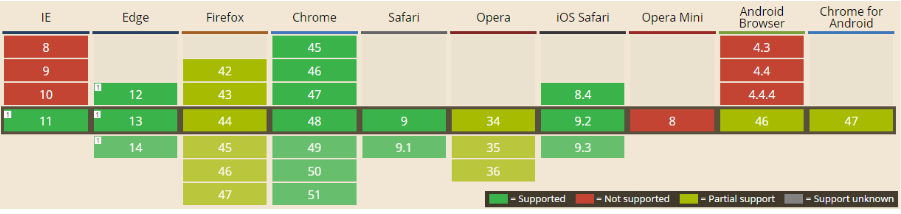
\includegraphics[width=0.8\linewidth]{images/chapter_tecnologie_abilitanti/tecnologie_abilitanti_webgl_compat.png}\hfill
 \caption[Lista browser compatibili]{Browser compatibili con WebGL.}
 \label{fig:stato_arte_webgl_compat}
\end{figure}
WebGL si basa sulle \emph{OpengGL ES 2.0}, librerie grafiche OpenGL ottimizzate per dispositivi mobili, che forniscono un’ interfaccia di programmazione per la grafica 3D. Utilizza l’ elemento canvas HTML5, che viene acceduto attraverso il DOM (Document Object Model), per renderizzare l’ immagine desiderata.
\\
Le API WebGL sono di basso livello e funzionano intuitivamente come una sequenza di messaggi da inviare all’ oggetto gl che rappresenta un contesto WebGL costruito su una canvas.
\begin{lstlisting}[language=JavaScript]
gl=document.getElementById("canvas_id").getContext("experimental-webgl");
\end{lstlisting}

Analizzare la pipeline di rendering di WebGL equivale praticamente ad analizzare la pipeline di OpenGL ES 2.0. Grazie a WebGL il programmatore non deve preoccuparsi dell’ intero processo di rendering in quanto alcune delle fasi più complesse vengono gestite dalla libreria.
La pipeline di WebGL è implementata per mezzo di Shader programmabili seguendo le specifiche di OpenGL ES 2.0 e di GLSL. Quest’ultimo è un linguaggio di programmazione ad alto livello per la gestione delle unità di shader di una GPU.
\\
Per shader si intende un’ insieme di istruzioni software che permettono di definire particolari operazioni ed effetti, come colorazione ed illuminazione, per il rendering degli elementi 3D della scena.
\\
In figura \ref{fig:tecnologie_abilitanti_webglrender}  è possibile osservare la pipeline di WebGL.La pipeline risulta simile a quella analizzata precedentemente in capitolo \ref{sec:chapter_stato_arte_open_gl}, ma presenta alcune differenze negli Shader.
\\
\begin{figure}[htb]
 \centering
 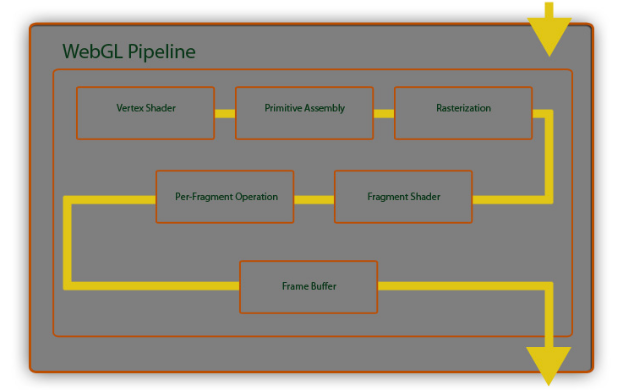
\includegraphics[width=1\linewidth]{images/chapter_tecnologie_abilitanti/tecnologie_abilitanti_webglrender.png}\hfill
 \caption[La pipeline di WebGL]{La pipeline di rendering WebGL}
 \label{fig:tecnologie_abilitanti_webglrender}
\end{figure}

Le specifiche WebGL richiedono che lo sviluppatore provveda a fornire alla GPU due shader chiamati rispettivamente Vertex Shader e Fragment Shader:
\begin{itemize}
\item Il Vertex Shader è un metodo programmabile il cui compito è quello di restituire, per ogni tripletta di coordinate che identificano un vertice nello spazio, una coppia di coordinate che identifichino lo stesso vertice sul piano bidimensionale dello schermo (la canvas). Tale operazione prende in considerazione le informazioni come il punto di vista e l’angolazione dalla quale viene osservata la scena.
\item Il Fragment Shader è un metodo programmabile il cui compito è quello di definire il colore di ognuno dei pixel della canvas sulla quale giace la rappresentazione bidimensionale della scena calcolata con le informazione del Vertex Shader. Tramite esso è possibile implementare effetti d’ illuminazione, effettuare il texture mapping, applicare le ombre oppure effetti come la rifrazione, riflessione o il bump mapping.
\end{itemize}
WebGL utilizza un dialetto del linguaggio di programmazione C chiamato GLSL per la definizione degli shaders. Questo linguaggio è stato appositamente realizzato per svolgere questo compito e per essere facilmente integrato in una pagina web.
\\
Un esempio di fragment shader è il seguente:


\begin{lstlisting}[language=html]
<script id="shader--fs" type="x-shader/x-fragment">
\end{lstlisting}
\begin{lstlisting}[language=javascript]
void main(void){
	gl_FragColor = vec4(1.0,1.0,1.0,1.0);
}
\end{lstlisting}
\begin{lstlisting}[language=html]
</script>
\end{lstlisting}

GLSL richiede che nella variabile \texttt{gl\_FragColor} venga inserito il colore con il quale viene renderizzato a video il pixel in oggetto. Se si utilizzasse lo shader creato nell’esempio tot su un modello tridimensionale, esso verrebbe visualizzato di colore bianco.
\\
Un vertex shader segue lo stesso approccio; la variabile da valorizzare in questo caso è chiamata \texttt{gl\_Position}.

\begin{lstlisting}[language=javascript]
void main(void){
	gl_Position = uPMatrix * uMVMatrix * vec4(aVertexPositionm 1.0);
}
\end{lstlisting}

Il problema di WebGL risiede però nella sua complessità.
Per disegnare un semplice triangolo bianco è necessario dichiarare le coordinate dei punti (x,y,z) che compongono i vertici (nove valori nell’ esempio).
Questi valori devono poi essere memorizzati all’ interno di un buffer utilizzato durante la fase di disegno.

\begin{lstlisting}[language=javascript]
function initBuffers() {
	triangleVertexPositionBuffer = gl.createBuffer();
	gl.bindBuffer(gl.ARRAY_BUFFER, triangleVertexPositionBuffer);

	var vertices = [ 0.0, 1.0, ...];

	gl.bufferData(gl.ARRAY_BUFFER, new Float32Array(vertices), gl.STATIC_DRAW);
	triangleVertexPositionBuffer.itemSize = 3;
	triangleVertexPositionBuffer.numItems = 3;
}
\end{lstlisting}
Successivamente per effettuare il rendering della scena su schermo sono necessarie ulteriori operazioni:

\begin{lstlisting}[language=javascript]
function drawScene() {
	gl.viewport(0, 0, gl.viewportWidth, gl.viewportHeight);
	gl.clear(gl.COLOR_BUFFER_BIT | gl.DEPTH_BUFFER_BIT);
	gl.bindBuffer(gl.ARRAY_BUFFER, triangleVertexPositionBuffer);

	gl.vertexAttribPointer(
		shaderProgram.vertexPositionAttribute,
		triangleVertexPositionBuffer.itemSize,
		gl.FLOAT, false, 0, 0);

	gl.uniformMatrix4fv(shaderProgram.pMatrixUniform, false, new Float32Array([1,0,0,0,....]));

	gl.uniformMatrix4fv(shaderProgram.uMVMatrixUniform, false, new Float32Array([1,0,0,0,..]));

	gl.drawArrays(gl.TRIANGLES, 0, triangleVertexPositionBuffer.numItems);
}
\end{lstlisting}
La funzione \texttt{DrawScene} nell’ esempio gestisce le operazioni necessarie per disegnare il triangolo nella canvas; nelle prime due righe viene resettata la scena, poi viene caricato nel contesto 3D il buffer contenente le informazioni dei vertici del triangolo e vengono impostati i parametri richiesti dagli shader.
Infine viene invocata la funzione \texttt{drawArrays} che disegna i vertici presenti nel buffer invocando per ognuno di essi gli shader.
\\
L’ esempio fornito, volutamente non completo, non vuole essere una spiegazione esaustiva di come usare WebGl, piuttosto risulta utile al fine di comprenderne la complessità di utilizzo.
\\
Disegnare un solo triangolo bianco e statico (senza alcuna animazione) è costato infatti circa 60 righe; a queste bisogna aggiungere ulteriori istruzioni di gestione del contesto WebGl sulla canvas scelta.
Le API WebGL risultano quindi decisamente troppo complesse e laboriose da utilizzare, soprattutto per la realizzazione di scene complesse. Scene complesse, come gli appartamenti 3D arredati costruiti nel presente lavoro di tesi.
\\
Three.js nasce con l’obiettivo di risolvere i problemi appena esposti e per facilitare il lavoro dello sviluppatore.



\section{Three.js}
\label{sec:chapter_tecnologie_abilitanti_threejs}

Three.js è una libreria/API JavaScript, basata su WebGL, che permette la creazione e visualizzazione di grafica 3D su browser web. Nasce con l’obiettivo di rendere WebGL facile da utilizzare.
La libreria Three.js permette di lavorare ad un livello più alto di astrazione rispetto a WebGL in quanto gestisce la fase di rendering per ogni oggetto nella scena, nascondendola di fatto al programmatore.
La libreria inoltre, occupandosi della matematica base, nasconde al programmatore la complessa algebra lineare delle trasformazioni come traslazione, rotazione o scalatura di un oggetto nella scena, permettendogli di utilizzare direttamente i risultati provenienti dai calcoli.
Di fatto questo velocizza il lavoro dello sviluppatore facendogli risparmiare parecchie linee di codice; un semplice cubo che con WebGL richiederebbe centinaia di righe di codice tra Javascript e GLSL per scrivere lo shader, in Three.js richiederebbe solo una piccola frazione di esse.
A questo punto verrà descritto un breve progetto Three.js al fine di presentarne la facilità di utilizzo rispetto a WebGL.
I progetti sviluppati in Three.js seguono tipicamente un approccio procedurale; per convenzione il codice viene sviluppato in tre funzioni: ‘init’, ‘animate’ e ‘render’ dividendo di fatto il progetto in tre segmenti logici: inizializzazione, aggiornamento e disegno.
\begin{lstlisting}[language=javascript]
var camera, scene, renderer;
init();
animate();

function init() {
 // sezione di set-up di progetto
}
function animate() {
 // sezione per l'aggiornamento e l'animazione
 requestAnimationFrame( animate );
 render();
}
function render() {
 // sezione di disegno su canvas
 renderer.render( scene, camera );
}
\end{lstlisting}
La funzione \texttt{animate()} utilizza il metodo \texttt{requestAnimationFrame()} che consente di invocare consecutivamente la funzione passata come parametro, nell’ esempio animate, all’ interno di un ciclo altamente ottimizzato dal browser. Questo ciclo permette al render di disegnare la scena al massimo per 60 volte al secondo, valore che però diminuisce all’aumentare della complessità della scena.
\\
Con un progetto completamente statico è possibile evitare l’invocazione della funzione animate ed accodare la funzione di disegno della scena a quella preposta all’ inizializzazione.
\\
A questo punto, per permettere a Three.js di effettuare il render su schermo sono necessari: un oggetto scena, un oggetto camera ed un renderer.
La scena permette di indicare quali oggetti renderizzare ed in quale posizione, semplicemente aggiungendoli e spostandoli all’interno di essa.
La camera indica quale porzione della scena viene renderizzata e mostrata su schermo. L’istanza di renderer è essenziale per indicare quale scena deve essere renderizzata da Three.js, e per definire la risoluzione della finestra del browser in cui viene mostrato il render.
\\ 
Infine viene aggiunto l’elemento renderer al documento HTML. Questo rappresenta l’elemento canvas che il renderer usa per mostrare la scena.
\\
Una volta inseriti i tre elementi, è necessario aggiungere alla scena l’elemento da renderizzare, ad esempio un cubo.
\begin{lstlisting}[language=javascript]
var geometry = new THREE.BoxGeometry(1,1,1);
var material = new THREE.MeshBasicMaterial({color: 0x00ff00});
var cube = new THREE.Mesh(geometry, material);
scene.add(cube);
\end{lstlisting}
Per fare questo bisogna inizializzare una Box Geometry, contenente le primitive geometriche fondamentali di un cubo.
\\
Oltre alla geometria bisogna creare un materiale che conferisce alcune proprietà all’oggetto. Esistono diversi materiali, ognuno con proprie caratteristiche, a cui si possono aggiungere proprietà che sono comuni ad ogni materiale come il colore. In questo esempio il materiale permette all’oggetto di assumere il colore verde.
\\ 
Infine bisogna creare la Mesh vera e propria che rappresenta l’oggetto con una propria geometria a cui è applicato un materiale. La mesh può essere inserita nella scena per essere renderizzata.
\\
L’esecuzione del codice nell’esempio permette la visualizzazione su schermo di un cubo statico verde.
\\
Risulta chiaro quindi quanto Three.js velocizzi e semplifichi il lavoro degli sviluppatori, risultando comprensibile anche a chi non comprende dettagliatamente la pipeline di rendering. Nel codice è totalmente assente l’ algebra lineare delle trasformazioni descritta tramite matrice. Per effettuare una traslazione è sufficiente indicare solamente la nuova posizione sugli assi $x$,$y$ o $z$ dell’ oggetto; Three.js nasconde al programmatore tutta la logica delle operazioni da effettuare sulla matrice di trasformazione per ogni traslazione, rotazione o scalatura. Inoltre effettua automaticamente la mappatura dalle coordinate 3D della scena a quelle 2D dello schermo, cosa che invece con WebGL sarebbe stata a carico del programmatore.
Three.js quindi, nel presente lavoro di tesi, è stato utilizzato come libreria base per la creazione dell’ editor e del navigatore di scene 3D fotorealistiche. I due ambienti verrano dettagliati nei capitoli successivi.


In conclusions...



%\part{Part 2}
\label{part:part_2}


%\chapter{Lightweight render loop}
\label{cha:chapter_lrl}

Nel paragrafo \ref{sec:chapter_tecnologie_abilitanti_webgl} è stato mostrato come nel browser venga utilizzato WebGL per usufruire dell’accelerazione grafica per il rendering 3D.
\\ 
Dal momento che, come per OpenGL, anche WebGL permette di interfacciarsi con le primitive solamente a basso livello, è necessario uno strumento che permetta di semplificare l’esperienza d’uso che altrimenti sarebbe fin troppo complessa, e Three.js è la soluzione a questo problema. Nonostante questa libreria contribuisca sensibilmente alla fruibilità di scene su browser, permangono tuttavia del problemi da risolvere: la scena deve avere una resa fotorealistica, e la fruizione della scena deve poter scalare su piattaforme multiple.
\\
Per fruire di una scena, avendo anche la possibilità di navigarla, è necessario effettuare il rendering in real-time; questo vuol dire che ad ogni ciclo di rendering tutte le informazioni sulla scena devono essere ricalcolate.
Utilizzare Three.js per rendere una scena fotorealistica è una pressochè impossibile, perchè nonostante fornisca tutti gli strumenti per aumentare l’impatto grafico di una scena, sarebbe computazionalmente oneroso utilizzarli in un contesto real-time.
Nel capitolo \ref{cha:chapter_stato_arte} è stato mostrato come uno degli elementi principali per migliorare la resa visiva di una scena sia l’illuminazione indiretta, e come gli algoritmi di illuminazione indiretta siano onerosi da calcolare.
\\
Un supporto per il calcolo real-time dell’illuminazione indiretta sul renderer di three.js sarebbe quindi inutilizzabile sulla stragrande maggioranza delle piattaforme. Generalmente le prestazioni di un rendering real-time risentono del numero di luci in una scena; questo perchè con l’aumentare delle luci, aumenta la quantità di informazioni di luci e ombre che la fase di vertex shading deve computare ad ogni ciclo.
Il fattore scalabilità è quindi fortemente influenzato dal numero di luci in una scena, specialmente in contesti come quello affrontato nel presente elaborato di tesi, dove si vogliono realizzare ambienti di dimensioni anche notevoli, come un’intera abitazione, e navigarli in prima persona.
\\
Per rendere scalabile il servizio di fruibilità della scena bisogna quindi ridurre il carico computazionale sulla pipeline di rendering, rendendola appunto “lightweight”, pur mantenendo la resa grafica fotorealistica.
A fronte di tale necessità verranno descritti gli accorgimenti adottati per velocizzare il ciclo di render.
Il primo accorgimento è quello di liberare la pipeline di rendering dal calcolo delle informazioni luminose, le quali verranno preprocessate offline una sola volta, e memorizzate all’interno di strutture dati chiamate \textbf{lightmapped texture} mediante il processo di baking; nel capitolo \ref{sec:chapter_lrl_li_te_ba} verrà spiegato cosa sono le lightmapped texture e quali caratteristiche la differenziano da una normale lightmap. 
\\
Siccome il calcolo dell’illuminazione non dipende più dal renderer di ThreeJS, può essere affidato ad uno strumento esterno, come un’applicazione desktop in grado di processare algoritmi di illuminazione complessi; ovviamente dovrà anche essere in grado di memorizzare i risultati ottenuti, processo di baking delle lightmap.
Un’altro dettaglio che incide profondamente sulle performance di un rendering è la presenza di effetti rifrangenti o riflettenti all’interno della scena. Ad esempio Three.js permette di creare degli specchi che riflettono l’ambiente circostante renderizzandolo in tempo reale.
Se all’interno della scena ci fossero degli oggetti in movimento, questi apparirebbero riflessi nella posizione in cui effettivamento si trovano.
\\
\begin{figure}[htb]
 \centering
 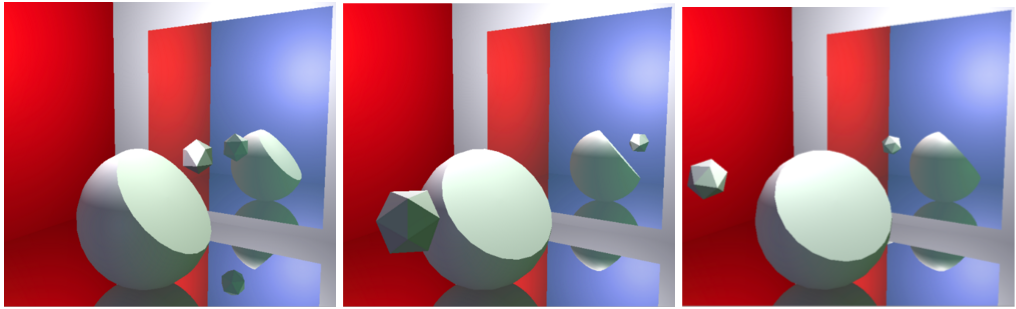
\includegraphics[width=0.9\linewidth]{images/chapter_lrl/lrl_specchio.png}\hfill
 \caption[ThreeJS Mirror]{In foto è possibile notare come lo specchio realizzato in ThreeJS rifletta in ogni istante di tempo gli oggetti della scena nelle posizioni in cui effettivamente si trovano.}
 \label{fig:lrl_specchio}
\end{figure}
\\
Nonostante il comportamento assolutamente realistico gli specchi risultano inutilizzabili se si vuole  alleggerire il carico di lavoro del renderer. Questo perchè per ogni specchio aggiunto una nuova pipeline di rendering dovrà essere eseguita, aumentando drasticamente la mole di lavoro da svolgere. Questa è sicuramente la soluzione meno scalabile perchè all’aumentare del numero degli specchi ci sarà bisogno di un hardware sempre più potente per mantenere fluida l’esperienza visiva. Se il contesto di utilizzo prevede scene prevalentemente statiche, è possibile  mantenere un’unica pipeline di rendering pur avendo effetti riflettenti o rifrangenti, utilizzando delle env-map. 
\\
Nel paragrafo \ref{sec:chapter_lrl_cond_app} verrano mostrate le condizioni che una scena deve soddisfare affichè il suo render possa essere reso leggero dalle soluzioni sopra mostrate.


\section{Condizioni di applicabilità}
\label{sec:chapter_lrl_cond_app}

Il lightweight render loop permette di diminuire drasticamente le operazioni effettuate dal ciclo di render quando viene calcolata una scena in cui sono presenti un elevato numero di luci e superfici riflettenti/rifrangenti.
\\
L’utilizzo delle informazioni di luci ed ombre precalcolate e salvate su lightmap e l’utilizzo delle env-map di riflessione e rifrazione è però possibile solo su scene statiche e immutabili nel tempo.
\\
Modificare una scena dopo che sono state applicate delle lightmap e delle env-map porterebbe ad un risultato fisicamente impossibile da osservare nella vita reale.
\\
È preferibile infatti evitare di modificare la posizione di oggetti che proiettano ombra su una scena in cui il bake è già stato effettuato in quanto l’ombra non si sposterebbe dinamicamente insieme all’oggetto. Essa piuttosto rimarrebbe fissa nella vecchia posizione.
\\ 
Inoltre l’oggetto spostato non proietterebbe nessuna ombra nella nuova posizione, rendendo di fatto la scena renderizzata non realistica. 
\\
Questo inconveniente viene ottenuto perchè le informazioni di luci ed ombre sono salvate all’interno delle lightmapped texture, ed all’interno del ciclo di render non viene effettuato alcun calcolo dinamico delle luci  (perchè le luci sono totalmente assenti nella scena).
\newpage
\begin{figure}[htb]
 \centering
 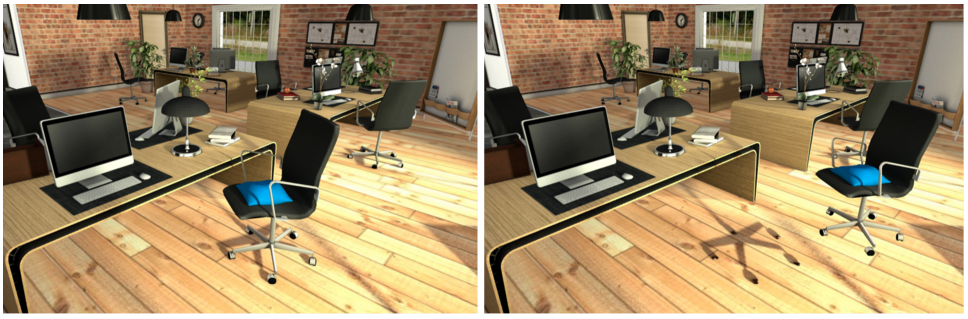
\includegraphics[width=1\linewidth]{images/chapter_lrl/lrl_appl1.png}\hfill
 \caption[Applicabilità, ombre statiche]{L' ombra sul pavimento rimane statica.}
 \label{fig:lrl_appl1}
\end{figure}
Stesso discorso per le env-map, modificare la scena dopo che le env-map sono state calcolate renderebbe irrealistici gli effetti di riflessione e rifrazione. Questo perchè le superfici continuerebbero a riflettere o rifrangere  il vecchio ambiente che risulterebbe diverso da quello modificato.
\begin{figure}[htb]
 \centering
 \includegraphics[width=1\linewidth]{images/chapter_lrl/lrl_appl2.png}\hfill
 \caption[Applicabilità, riflesso con env map]{Uno specchio ottenuto tramite una env map riflettente. Il riflesso risulta però immutibile nonostante lo spostamento degli oggetti.}
 \label{fig:lrl_appl2}
\end{figure}
\\
Proprio per questi motivi è possibile ottenere scene fotorealistiche e scalabili solamente se esse, una volta create, non vengono modificate nel tempo.
\\
Questo di fatto non rappresenta una limitazione per il presente lavoro di tesi in quanto l’applicazione creata è rivolta principalmente ad architetti per la creazione di appartamenti fotorealistici.
\\
Gli appartamenti infatti una volta progettati ed arredati risultano completamente statici nel tempo in quanto in essi sono totalmente assenti animazioni, come lo spostamento di un oggetto.
\\
Quindi per l’architetto è sufficiente creare l’appartamento, scegliere da dove provengono le luci, inserire gli effetti di riflessione/rifrazione ed avviare il processo di bake.
Siccome questi effetti così come le luci influenzano l’intero appartamento, esattamente come nel mondo reale, è necessario che la scena creata sia completamente computata durante il processo di bake. 
\\
Se ad esempio venisse processato un bake diverso per ogni singola stanza, il risultato ottenuto non risulterebbe completamente corretto in quanto luci ed ombre posso conivolgere insieme più stanze e gli effetti di riflessione/rifrazione in una stanza possono dipendere da altre stanze.
\\
\begin{figure}[htb]
 \centering
 \includegraphics[width=1\linewidth]{images/chapter_lrl/lrl_appl3.png}\hfill
 \caption[Applicabilità, scene autocontenute]{Effetti di luce fotorealistici ottenuti tramite un unico bake dell'intera scena.}
 \label{fig:lrl_appl3}
\end{figure}
Questo ragionamento può essere applicabile solo su porzioni di scena autocontenute, come ad esempio una stanza chiusa di un appartamento, in cui è impossibile che luci, ombre ed effetti di riflessione/rifrazione possano influenzare altre stanze.
Nulla vieta comunque l’applicazione totale o parziale di questa tecnica su scene dinamiche, in cui il beneficio ottenuto dal miglioramento delle prestazioni è talmente elevato da giustificare  risultati non completamente realistici. 

\section{Lightmapped texture baking}
\label{sec:chapter_lrl_li_te_ba}

Nel paragrafo \ref{sec:chapter_stato_arte_lightmap} si è già discusso di lightmap, e di come queste vengono realizzate.
Le lightmapped texture sono di base delle lightmap, ma con delle differenze sia nelle proprietà che nel processo costruttivo. 
\\
Come già accennato nell’introduzione, per il baking di queste lightmapped texture si è fatto uso di uno strumento esterno in grado di computare algoritmi di illuminazione complessi senza coinvolgere il real-time rendering di Three JS. La scelta è ricaduta sul software di grafica 3D Blender, il quale dispone di algoritmi di illuminazione indiretta per una resa grafica notevole, come il Path Tracing. Inoltre la realtà open source del programma ha permesso di modellarne dei comportamenti, per venire incontro a delle esigenze di utilizzo che verrano mostrate nei capitoli più avanti. Blender permette di eseguire l’unwrap dei modelli 3D e quindi di produrre le mappe UV di cui si è già discusso nel paragrafo \ref{sec:chapter_stato_arte_lightmap}. 
\\
\begin{figure}[htb]
 \centering
 \includegraphics[width=1\linewidth]{images/chapter_lrl/lrl_unwrap.png}\hfill
 \caption[Blender unwrap]{Processo di unwrap in Blender.}
 \label{fig:lrl_unwrap}
\end{figure}
Il processo di baking delle lightmap prevede nella stragrande maggioranza dei casi che le UV Map utilizzate siano quelle generate dal software in uso. Ci sono tuttavia dei casi dove questa potrebbe non essere la soluzione ottimale.
Quando si crea una scena è possibile importare dei modelli creati da terze parti; ogni modello è rappresentato da un file obj contenente le primitive geometriche del modello (vertici, spigoli e facce), le coordinate UV, e le normali. Inoltre al file obj viene allegata la diffuse texture pensata per il modello dal creatore dello stesso.

Le coordinate UV del modello sono realizzate per consentire un mapping ottimale della diffuse texture sulle superfici 3D dell’oggetto. Siccome quindi l’UV Map già esiste, ed è ottimizzata per il modello, è possibile esulare Blender dall’eseguire l’unwrap, evitando quindi di generare una mappa UV diversa, a favore di quella preesistente. 
Ovviamente qualora mancasse la mappa UV di un modello, l’unwrap sarà necessario. 
Utilizzando per la lightmap la stessa UV Map usata per mappare la diffuse texture si avrà che:  se un texel $T$ nella diffuse texture copre la posizione $(u1,v1)$, e un lumel $L$ copre la stessa posizione $(u1,v1)$ nella lightmap, allora $L$ e $T$ saranno mappati sullo stesso frammento del modello 3D.
Quindi diffuse texture e lightmap sono completamente sovrapponibili, e il mapping sul modello 3D sarà ottimale per le lightmap così come lo è per la diffuse texture.
I vantaggi di una scelta simile sono soprattutto a livello qualitativo. 
Nel paragrafo \ref{sec:chapter_stato_arte_lightmap} si è già fatto cenno a come i software di grafica 3D permettano all’artista di intervenire sul processo di unwrap, per modellare a mano l’UV map generata dal software nei punti dove il mapping può aver commesso degli errori; questo può accadere con geometrie complesse, specialmente in punti dove la superficie del modello è curva. 
Nel presente lavoro di tesi si assume che la mappa UV realizzata dal creatore del modello sia quella ottimale, in quanto creata appositamente per quell’oggetto. Una procedura completamente automatizzata infatti difficilmente riuscirebbe a raggiungere lo stesso risultato.
\\
\begin{figure}[htb]
 \centering
 \includegraphics[width=1\linewidth]{images/chapter_lrl/lrl_diff_uvmap.png}\hfill
 \caption[Confronto UV Map]{In foto viene mostrata una mappa uv generata automaticamente da Blender (a sinistra), e una mappa uv creata dall'artista del modello (a destra).}
 \label{fig:lrl_diff_uvmap}
\end{figure}
Nel contesto del presente elaborato di tesi il software di grafica 3D è completamente trasparente all’utente. Pertanto le uniche UV Map in possesso sono quelle generate da Blender in modo completamente automatico o quelle create da terzi per i modelli importati, per le quali invece il creatore potrebbe aver avuto la possibilità di intervenire a mano per migliorarle.
\\
Generalmente le informazioni luminose calcolate offline vengono memorizzate in una struttura dati separata dalla diffuse texture, in modo da poter usare l’una indipendentemente dall’altra, e sfruttare la riusabilità delle diffuse texture.
\\ 
Tuttavia allo stato attuale è previsto un unico setup di illuminazione all’interno della scena, anche se la flessibilità del sistema permetterebbe l’installazione di un supporto per diversi setup di illuminazione all’interno della stessa scena, come il ciclo giorno/notte.  Avere per uno stesso appartamento setup di illuminazione diversi è utile specialmente per branche dell’architettura come l’illuminotecnica. Pertanto il fattore riusabilità di una texture, di cui si è fatto cenno nel paragrafo \ref{sec:chapter_stato_arte_lightmap}, diventa superfluo. In questo caso ha poco senso mantenere elementi di immagine e di luce in strutture dati separate, e quindi grazie alla sovrapponibilità delle due strutture dati si può ottenere un’unica texture dove in ogni texel i valori RGB della diffuse texture sono moltiplicati per i valori di irradianza memorizzati nei lumel della lightmap. Questa nuova struttura dati viene detta lightmapped texture. 
\\
\begin{figure}[htb]
 \centering
 \includegraphics[width=1\linewidth]{images/chapter_lrl/lrl_li_te.png}\hfill
 \caption[Lightmapped texture]{Confronto tra una normale diffuse texture (a sinistra), e relativa lightmapped texture (a destra)}
 \label{fig:lrl_li_te}
\end{figure}
Il software Blender permette la creazione di lightmapped textures, specificando la modalità di bake “combined”; questa modalità emula ciò che si avrebbe con render completo del modello, e quindi produce in output la combinazione tra luce e colore diffuse del modello.

In conclusions...



%\chapter{Architettura del sistema}
\label{cha:chapter_architettura_sistema}

Il contesto applicativo a cui si rifersce il sistema trattato nel presente lavoro di tesi è prevalentemente architetturale.
All’interno di tale contesto l’obiettivo è quello di garantire all’utente la possibilità di costruire ambienti 3D fotorealistici e di fruirne mediante navigazione degli interni, il tutto mediante servizio web. 
Nonostante siano molte le applicazioni di grafica 3D che permettono di realizzare e rendere fotorealistiche delle scene, nella maggior parte dei casi queste sono applicazioni desktop, come Blender.
Per utilizzare un’applicazione desktop di grafica 3D è necessario:
\begin{itemize}
\item Installare il software.
\item Mantenere aggiornato il software.
\item Comprendere l’interfaccia, che in software di questo tipo può risultare complessa.
\item Imparare ad usare gli strumenti che il software offre per realizzare una scena, quindi:
\begin{itemize}
\item Inserire nuovi oggetti o importarne di gia esistenti.
\item Inserire luci o camere.
\item Importare modelli preesistenti. 
\item Texturizzare gli oggetti.
\item Scegliere il tipo di renderer.
\item Imparare il processo di baking delle lightmap.
\end{itemize}
\end{itemize}
Tutto ciò difficilmente rappresenterebbe un problema per un utenza già avvezza con questo tipo di software, ma spesso si ha a che fare con utenti alle prime armi, che non conoscono bene il panorama dei software di grafica 3D e che quindi si ritrovano a dover provare software diversi, rischiando di ripetere i passi sopra descritti più di una volta. 
\\
Sperimentando con mano l’utilizzo di un software come Blender ci si rende effettivamente conto di quanto procedure come il baking delle lightmap richiedano uno studio preventivo.
\\
Inoltre l’utente potrebbe sentirsi limitato nell’uso di strumenti di questo tipo per motivi prettamente legati all’hardware.
Ad esempio il baking delle lightmap prevede che per ogni oggetto della scena venga eseguito un render completo, e per la realizzazione di scene fotorealistiche questo render è un processo oneroso e di durata sensibilmente variabile a seconda dell’hardware di accelerazione grafica a disposizione. 
\\Questo limita la maggior parte degli utenti che intendono realizzare scene fotorealistiche complesse, in quanto non possessori di un hardware adatto allo scopo. Sulla base di queste motivazioni si è deciso di realizzare un ecosistema che venisse incontro a tutte le esigenze degli utenti per la realizzazione e la navigazione di interni 3D fotorealistici, garantendo semplicità d’uso e prestazioni compatibili con la maggior parte degli hardware di accelerazione grafica. 
\\
Le carattestistiche fondamentali di questo sistema sono:
\begin{itemize}
\item Separazione delle responsabilità funzionali di realizzare, rendere fotorealistca, e navigare la scena, incapsulandole in moduli implementati e mantenuti come entità a se stanti.
\item Realizzazione  web-based del servizio, con architettura client-server. 
\end{itemize}
L’implementazione di moduli autocontenuti in ambiente web permette all’utente di interfacciarsi solamente con le funzionalità di cui ha bisogno direttamente da browser, rimanendo all’oscuro di dettagli tipici nelle applicazioni desktop come l’installazione di software o aggiornamenti. Ogni modulo corrisponde ad un servizio separato; il sistema in tutto ne prevede tre:
\begin{itemize}
\item L'\textbf{Editor}, che incapsula le responsabilità funzionali di realizzare una scena, e mediante interfaccia semplice ed intuitiva offre tutte le funzioni tipiche di un ambiente di editing 3D, renderizzando dinamicamente il risultato su schermo. Il servizio di Editor è accessibile da browser mediante apposita URL.
\item Il \textbf{Navigator}, che incapsula le responsabilità funzionali di navigazione di una scena, e anche qui il servizio offre un’interfaccia attraverso la quale poter cambiare modalità di navigazione, e importare o rimuovere la scena. Il servizio di Navigator è accessibile da browser mediante apposita URL.
\item Il \textbf{Baking Service}, che rappresenta la funzionalità peculiare del nostro sistema, ciò che permette, data una scena con un determinato setup di illuminazione, di ottenere una scena fotorealistica mediante processo di baking delle lightmap su ogni oggetto della scena. A differenza dell’Editor e del Navigator, il servizio di bake è accessibile mediante feature presente all’interno dell’editor.
\end{itemize}
La caratteristica che più contraddistingue tale sistema dalla media dei servizi di editing 3D online che si trovano sul web, è proprio il Baking Service.
\\
Questo servizio è stato realizzato appositamente per permettere all’utente di effettuare il bake delle lightmap senza però preoccuparsi di alcun dettaglio circa il modo in cui il bake verrà effettuato. L’utente non ha bisogno di imparare come si fa il baking delle lightmap, e non deve installare alcun software; mediante l’interfaccia offerta dall’Editor è sufficiente premere un bottone, semplificando drasticamente l’esperienza d’uso. 
\\
Nascondere all’utente gli aspetti più onerosi dell’esecuzione di un bake non è l’unico grande vantaggio di un servizio simile; sfruttando infatti l’architettura client-server è possibile installare il servizio di bake su un nodo fisico completamente diverso da quello sul quale l’utente sta realizzando la scena.
\\ 
Siccome il bake prevede il processamento di algoritmi di illuminazine complessi, si predispone quindi una macchina con una configurazione hardware di fascia alta, il cui compito è esclusivamente quello di effettutare il baking e restituire il risultato. 
\\
L’Editor si occuperà di trasformare la richiesta di bake dell’utente in una richiesta al servizio remoto in modo completamente trasparente all’utente.
\\ 
Questa caratteristica estende la possibilità di far richiesta di bake onerosi anche a computer che non hanno i requisiti sufficienti per far girare il processo in locale. 
\\
Nonostante la parte computazionalmente più onerosa, ovvero il bake, sia assegnata ad un nodo di calcolo differente da quello in uso dall’utente, si consideri che l’Editor, così come il Navigator, girano sul client; questo vuol dire che la complessità computazionale del rendering real-time di ThreeJS è tutta a carico dell’hardware su cui l’utente sta creando, o navigando la scena. 
\\
Il vantaggio è però quello di avere lato client solamente la pipeline di rendering “lightweight”. L’incapsulamento delle responsabilità funzionali in moduli differenti permette di organizzare il codice in modo che l’intero sistema sia flessibile ai cambiamenti durante il corso della sua vita, e permette inoltre di poter apportare interventi mirati all’implementazione di uno specifico servizio, senza dipendere dai dettagli implementativi di altri moduli. Le uniche dipendenze presenti tra i servizi sono nelle interfacce che questi espongono.
\\  
A questo punto è possibile individuare tre servizi implementati in modo completamente diverso tra loro; mentre l’Editor e il Navigator si basano sulla stessa tecnologia, ovvero ThreeJS, Baking Service è un entità completamente diversa, scritta in Python. 
\\
Ciononostante i tre servizi devono comunicare; in particolare la scena creata nell’Editor deve poter essere inviata al servizio remoto di baking, e lo stesso servizio deve fornire in output un dato comprensibile sia dall’Editor che dal Navigator. 
\\
Per consentire questo scambio di informazioni si è scelto un formato comune di interscambio dei dati, ovvero il JSON, e su ogni servizio è stato implementato un supporto per il riconoscimento del formato. Per semplificare l’installazione dei supporti al formato si è partiti da standard di formati JSON già definiti in ThreeJS per la descrizione di scene; studiando tutte le possibilità offerte si è arrivati a scegliere lo standard che meglio si adattasse al presente lavoro di tesi. 
\\
Nel paragrafo \ref{sec:chapter_architettura_sistema_formato_scambio} verrà mostrato un modo per riuscire a descrivere in un unico file tutte le informazioni presenti in una scena generata nell’Editor, ed elaborata dal servizio di bake.

\section{Section 2}
\label{sec:chapter_architettura_sistema_il_servizio}

In this section...

\section{Formato di scambio dei dati}
\label{sec:chapter_architettura_sistema_formato_scambio}

Per permettere la comunicazione delle  tre componenti principali (servizio, editor, navigatore) del sistema creato per il presente lavoro di tesi è stato utilizzato un formato di scambio di dati completamente indipendente dal linguaggio di programmazione: JSON (JavaScript Object Notation).
Questo formato si basa sul linguaggio JavaScript ed utilizza testo, semplice da leggere e scrivere, per trasmettere dati costituiti da coppie attributo-valore (oggetti).
\\
Esso rappresenta il formato  di dati più usato per permettere la comunicazione asincrona tra browser/server, questo perchè utilizza convenzioni conosciute dai programmatori Java, Javascritpt, C, Perl, Python per citarne alcuni. Questa caratteristica rende di fatto il JSON un linguaggio ideale per lo scambio di dati ed ha consentito in questo lavoro la comunicazione tra un’ applicazione browser lato client scritta in Javascript (sia l’ editor che il navigatore) ed il servizio lato server scritto in Python.
\\
Il formato JSON è basato su due strutture di dati universali:
\begin{itemize}
\item Un insieme di coppie nome/valore. In base al tipo di linguaggio utilizzato esse possono rappresentare un oggetto, un record, una struct, un dizionario, una tabella hash, un elenco di chiavi, un array associativo.
\item Un elenco ordinato di valori. Nelle maggior parte dei linguaggi essi rappresentano un array o un vettore.
\end{itemize}

Nello specifico queste strutture vengono rappresentate tramite oggetti, array e valori:
\begin{itemize}
\item Un oggetto è una serie non ordinata di nomi/valori che inizia con una parentesi graffa sinistra e termina con una destra. Ogni nome è seguito dai due punti ed i valori sono separati dalla virgola.
\begin{figure}[htb]
 \centering
 \includegraphics[width=0.9\linewidth]{images/chapter_architettura_sistema/oggetto_json.png}\hfill
 \caption[Un oggetto JSON]{Un oggetto JSON}
 \label{fig:architettura_sistema_oggetto_json}
\end{figure}
\item Un elenco ordinato di valori. Nelle maggior parte dei linguaggi essi rappresentano un array o un vettore.
\begin{figure}[htb]
 \centering
 \includegraphics[width=0.9\linewidth]{images/chapter_architettura_sistema/array_json.png}\hfill
 \caption[Un array JSON]{Un array JSON}
 \label{fig:architettura_sistema_array_json}
\end{figure}
\item Un valore può essere di tipo booleano (true, false), un numero (intero, reale o in virgola mobile), una stringa, un oggetto o un array. Queste strutture possono essere annidate.
\begin{figure}[htb]
 \centering
 \includegraphics[width=0.9\linewidth]{images/chapter_architettura_sistema/valore_json.png}\hfill
 \caption[Un valore JSON]{Un valore JSON}
 \label{fig:architettura_sistema_valore_json}
\end{figure}

\end{itemize}

Inoltre sono disponibili funzioni, scritte in diversi linguaggi di programmazione tra cui JavaScript e Python, che permettono facilmente di effettuare il parsing e la scrittura del formato dati JSON. Questa caratteristica è stata sfruttata in questo elaborato ed ha agevolato il lavoro di lettura e scrittura del JSON.
Tramite l’utilizzo di queste strutture dati all’interno del JSON è possibile definire il proprio formato di scambio (uno standard), creato appositamente per il trasferimento dei dati voluti.
Three.js definisce infatti il proprio standard tramite due formati differenti: il formato JSON 3 ed il formato JSON 4. 
\\
Entrambi i formati sono stati oggetto di profondo studio nel presente lavoro, questo ha permesso di valutare quale tra i due si addicesse meglio ad essere utilizzato all’interno dell’ecosistema creato. 

\subsection{I due formati di Three.js}
Attualmente in Three.js sono definiti due standard differenti per il trasferimento di dati: il formato JSON 3 e JSON 4. Di fatto questi formati descrivono la metodologia con cui deve essere scritto il file di testo affinché il parser possa riconoscere correttamente le informazioni inserite.
Nello specifico il file utilizzato per lo scambio di dati risulta differente in base a quale dei due formati è stato scelto, inoltre ad ogni formato corrisponde uno specifico parser che viene utilizzato per analizzare il testo.
\\
In Three.js risultano già definiti due differenti parser in grado di analizzare i formati JSON 3 e JSON 4. I due analizzatori presentano caratteristiche differenti, che verrano dettagliate successivamente. Inoltre entrambi i formati ed i corrispettivi parser risultano incompleti in quanto non permettono di trasferire alcune strutture dati Three.js, essenziali per questo lavoro di tesi.
Nel presente lavoro inoltre entrambi i formati di scambio sono stati studiati accuratamente per permettere di scegliere quali tra i due meglio si addicesse per l’architettura client/server sviluppata.
\\
In particolare Three.js ha un parser JSON 3 che permette di analizzare (un importer) un formato di questo tipo ma non di scriverlo (un exporter), mentre Blender presenta dei plug-in che permettono di utilizzare un parser sia per la lettura che per la scrittura.
\\
Invece per quanto riguardo il formato JSON 4; Three.js ha un parser che ne permette sia la lettura che la scrittura , mentre Blender ha un plug-in che permette di utilizzare il parser per la sola scrittura di questo formato.
\\
La scelta di quale formato utilizzare è risultata quindi fondamentale al fine di comprendere cosa sviluppare per permettere lo scambio completo dei dati da Three.js verso Blender e da Blender verso Three.js.
Con il formato JSON 3 era necessario creare un exporter scritto nel linguaggio Three.js, mentra con il formato JSON 4 era necessario creare un importer in Blender scritto con il linguaggio Python.
Quest’ultima  tra le due risultava la soluzione più complessa da realizzare in quanto necessitava lo studio di una libreria completamente nuova (quella di Blender) scritta in Python.
Nonostante la maggiore complessità questa soluzione è stata quella adottata in quanto il formato JSON 4 , rispetto al JSON 3, meglio si addiceva al contesto di questo lavoro.
\\
In questo capitolo verranno quindi esaminati i vantaggi e gli svantaggi dei due formati e dei rispettivi parser, verrà inoltre motivata la scelta che ha portato all’utilizzo di un formato piuttosto che di un’altro e verranno descritte le modifiche ed i miglioramenti apportati al formato scelto.

\subsection{Il formato JSON 3}
Il formato JSON 3 permette il trasferimento di dati Three.js attraverso un file di testo molto difficile da scrivere e da leggere. 
Questa difficoltà si ripercuote direttamente sul parser, rendendolo di fatto molto complesso e poco modificabile.
Durante il presente lavoro di tesi è stato confermato che il formato JSON 3 verrà presto deprecato in favore del nuovo formato JSON 4.
\\
Nonostante questo, studiare i vantaggi e gli svantaggi del formato JSON 3 si è reso necessario per poter prendere alcune importanti decisioni progettuali, descritte nell'introduzione al capitolo.
Viene adesso fornito un piccolo esempio di file scritto nel formato JSON 3 in cui vengono riportate le informazioni di due piani (uno blu ed uno rosso) insieme ai corrispondenti parametri di renderizzazione.

\begin{lstlisting}[language=json]
{ 
	"metadata" :{"formatVersion" : 3.1},
	"materials" : [{
		"DbgColor" : 15658734,
		"DbgIndex" : 0,
		"colorDiffuse" : [0, 0, 1],
		"shading" : "Lambert",
		"transparency" : 1.0,
		"trasnparent" : true,
	},{
	"materials" : [{
		"DbgColor" : 15658734,
		"DbgIndex" : 1,
		"colorDiffuse" : [1, 0, 0],
		"shading" : "Lambert",
		"transparency" : 0.5,
		"trasnparent" : true,
	}],
	"vertices" : [1,0,1,1,0,-1...],
	"normals" : [0.1.0],
	"uvs" : [],
	"faces" : [34,0,1,2,0,0,0,0, 34,3,0,2,0,0,0,0, ...]
}
\end{lstlisting}
I parametri fondamentali (visibili nell’esempio) sono:
\begin{itemize}
\item \texttt{materials}: un array di materiali da assegnare ai corrispondenti oggetti dove per ogni materiale vengono descritte le proprietà da esso possedute.
\item \texttt{vertices}: un array di vertici descritti in coordinate mondo. All’interno di questo array sono presenti i vertici di tutti gli oggetti nella scena da renderizzare.
\item \texttt{normals}: un array in cui vengono inserite le normali. Ogni normale è un vettore rappresentato mediante i tre valori (x,y,z). All’interno di questo array sono presenti le normali di tutti gli oggetti nella scena.
\item \texttt{colors}: un array in cui sono descritti i colori delle facce di ogni oggetto presente nella scena.
\item \texttt{uvs}: un array che contiene le coordinate uv di ogni oggetti della scena.
\item \texttt{faces}: un array complesso in cui sono riportate le informazioni di tutte le facce degli oggetti nella scena. In questo array sono presenti dei codici univoci che permettono di descrivere la tipologia di tutte le facce inserite.
\end{itemize}

Il parametro faces risulta il più complesso tra quelli presentati e proprio da quest’ultimo il parser inizia ad analizzare il JSON.
Questo formato si basa infatti sull’utilizzo di una complessa bitmask che permette al parser, a partire dai codici univoci presenti nell’array faces, di riconoscere il numero di vertici che compongono le facce e le caratteristiche che esse possiedono. 
Il codice univoco viene prelevato, convertito in  binario e poi sovrapposto sulla bitmask.
\\
La bitmask utilizzata è la seguente:
\begin{itemize}
\item $00 00 00 00$ = \texttt{TRIANGLE} (3 valori)
\item $00 00 00 01$ = \texttt{QUAD} (4 valori)
\item $00 00 00 10$ = \texttt{FACE\_MATERIAL} (1 valore)
\item $00 00 01 00$ = \texttt{FACE\_UV} (1 valore)
\item $00 00 10 00$ = \texttt{FACE\_VERTEX\_UV} (3 valori se triangolo, 4 altrimenti)
\item $00 01 00 00$ = \texttt{FACE\_NORMAL} (1 valore)
\item $00 10 00 00$ = \texttt{FACE\_VERTEX\_NORMAL} (3 valori se triangolo, 4 altrim.)
\item $01 00 00 00$ = \texttt{FACE\_COLOR} (1 valore)
\item $10 00 00 00$ = \texttt{FACE\_VERTEX\_COLOR} (3 valori se triangolo, 4 altrimenti)
\end{itemize}
Al fine di comprendere meglio il funzionamento della bitmask verrà fornito un esempio:

``faces'' : [34,\textcolor{red}{0,1,2,}\textcolor{blue}{0,}\textcolor{purple}{0,0,0,}    34,\textcolor{red}{3,0,2,}\textcolor{blue}{0,}\textcolor{purple}{0,0,0,}    34,\textcolor{red}{4,5,6,}\textcolor{blue}{1,}\textcolor{purple}{0,0,0,}   34,\textcolor{red}{6,4,5,}\textcolor{blue}{1,}\textcolor{purple}{0,0,0}]
Come riportato precedentemente nell’array faces sono rappresentate le diverse facce che compongono l’oggetto da renderizzare. 
Ogni faccia è descritta medianti diversi valori nell’ array, il numero di valori dell’array da assegnare alla faccia e cosa rappresentano questi valori viene indicato dal codice univoco in questo caso 34.
\\
Nell’esempio infatti il codice 34 viene convertito nel binario 00100010 e poi sovrapposto sulla bitmask. La sovrapposizione viene effettuata bit a bit a partire da destra verso sinistra.
Nell’ ordine da destra verso sinistra avvengono quindi le seguenti tre sovrapposizioni con il binario 00\textcolor{purple}{1}000\textcolor{blue}{1}\textcolor{red}{0}:

\begin{itemize}
\item \texttt{Triangle} (primo zero a partire da destra): la faccia quindi è costituita da tre vertici (in rosso nell'esempio) e rappresenta quindi un triangolo e non un quadrato. Siccome è la prima sovrapposizione nell’array faces i tre valori dopo il codice rappresentano tre indici da utilizzare nell’array vertices.
\item \texttt{Face Material} (primo uno a partire da destra): alla faccia quindi è associato un materiale. Siccome è la seconda sovrapposizione, nell’array faces il valore dopo le tre cordinate (in blu nell'esempio) rappresenta un indice da utilizzare nell’array materials.
\item \texttt{Face Vertex Normal} (secondo uno a partire da destra): alla faccia sono associate delle normali di vertice. Siccome è la terza sovrapposizione i 3 valori dopo l’indice del materiale (in viola nell'esempio) rappresentano le normali di vertice. La prima normale è associata al primo vertice, la seconda normale al secondo vertice e la terza normale al terzo vertice.
\end{itemize}

Le tre sovrapposizione calcolate permettono di indicare al parser il numero di indici (oltre al codice) da considerare per la faccia, in base al codice ad essa assegnato; in questo caso 7 (3+1+3). 
Questo permette di fatto al parser di distringuere le diverse facce presenti nell’array.
\\
Inoltre è utile specificare come  i vertici, nel punto 1, vengono prelevati dall’array a triplette; ad esempio per l’indice 0 vengono prelevati i tre valori a partire dalla posizione zero mentre per l’indice 1 i tre valori a partire dalla posizione tre e così via. I tre valori presi rappresentano infatti, nell’ ordine, il valore della coordinata (x, y, z).
Stesso discorso per il punto 2 dove le normali nell’array normals sono prelevate a triplette.

Le tre sovrapposizione calcolate permettono di indicare al parser il numero di indici (oltre al codice) da considerare per la faccia in base al codice ad essa assegnato, in questo caso 7 (3+1+3). 
Questo permette di fatto al parser di distringuere le diverse facce presenti nell’array.
I vertici, nel punto 1, vengono prelevati dall’array vertices tramite gli indici (rossi nell’esempio) inseriti dopo il codice. Ad esempio se l’indice è uguale a 0 vengono prelevati i tre valori a partire dalla posizione zero, mentre se l’indice è uguale ad 1 vengono presi i tre valori a partire dalla posizione tre. Essi rappresentano infatti, nell’ ordine, il valore della coordinata (x, y, z).
Stesso discorso per il punto 2 dove le normali nell’array normals sono prelevate a triplette.
\\
Viene ora fornito un ulteriore esempio, in cui vengono utilizzate facce quadrangolari invece che triangolari. Inoltre viene esaminata la modalità di utilizzo dell’array colors.
\\
Il codice inserito nell' array faces per questo esempio è 65.

\begin{lstlisting}[language=json]
{ 
"metadata" : { "formatVersion" : 3 }, 
"materials" : [], 
"vertices" : [ -5,5,-5, -5,-5,-5, 5,-5,-5, 5,5,-5, -5,5,5, -5,-5,5, 5,-5,5, 5,5,5 ], 
"faces" : [ 65,3,2,1,0,0, 65,4,5,6,7,1, 65,7,6,2,3,2, 65,0,1,5,4,3, 65,0,4,7,3,0, 65,6,5,1,2,1 ], 
"colors": [ 16711680, 65280, 255, 16776960 ], 
"normals": [], 
"uvs": [] 
}
\end{lstlisting}

Anche per questo esempio verrà analizzata una faccia dell'array faces:

``faces'' : [65,\textcolor{red}{3,2,1,0,}\textcolor{blue}{0,}]

Il codice viene convertito nel binario 01000001 e sovrapposto sulla bitmask.
Nell’ ordine da destra verso sinistra avvengono due sovrapposizioni con il binario 0\textcolor{blue}{1}00000\textcolor{red}{1}:

\begin{itemize}
\item \texttt{Quad}(primo uno a partire da destra): la faccia quindi è costituita da quattro vertici e rappresenta quindi un quadrato e non un triangolo. Siccome è la prima sovrapposizione nell’array faces i quattro valori dopo il codice rappresentano tre indici da utilizzare nell’array vertices.
\item \texttt{Face color} (secondo uno a partire da destra): alla faccia è associato un colore descritti nel formato decimale; in questo caso 16711680 = 0xff0000. Siccome è la seconda sovrapposizione il valore dopo i quattro vertici rappresenta l’indice da utilizzare per prelevare il colore della faccia dall’array colors.
\end{itemize}
Le due sovrapposizione calcolate permettono di indicare al parser che il numero di indici oltre al codice da considerare per la faccia sono 5 (4+1). 
\\
La trattazione del JSON 3 nel presente paragrafo non è volutamente esaustiva ma risulta particolarmente adatta per mostrare i problemi che derivano dall’utilizzo di questo formato di scambio.
\\
Lo standard risulta infatti molto complesso sia da scrivere che da leggere, complessità che aumenta esponenzialmente all’incrementare del numero di oggetti presenti nella scena.
\\
Siccome viene utilizzato un array di vertici ed uno di facce per tutti gli oggetti, tali array con l’incrementare del numero oggetti diventano talmente popolati da risultare di fatto incomprensibili. Per una persona che legge questo formato risulta difficile comprendere non solo quanti e quali oggetti sono presenti nella scena ma anche a quali oggetti associare i parametri di rendering. 
Questo rende difficile modificare a mano un file di testo scritto tramite questo formato.
\\
Inoltre il fatto che tutto sia scritto all’interno di questi array non permette di riportare all’interno del formato di scambio la descrizione gerarchica degli oggetti presenti nella scena.
Descrizione però fondamentale per questo elaborato al fine di mantenere inalterata la scena durante lo scambio di informazioni tra editor e servizio. 
\\
La gerarchia permette alle persone che utilizzano il sistema creato in questo lavoro di tesi di abbracciare un approccio iterativo incrementale. infatti se venisse salvata una scena nel formato JSON 3 e poi quest’ultimo venisse caricato, tutta la gerarchia associata agli oggetti andrebbe persa. Inconveniente non voluto in quanto la scena salvata deve risultare assolutamente identica a come è stata creata.
\\
Infine il parser del JSON 3, descritto in [riferim], risulta non solo molto complesso ma anche poco modificabile. La modificabilità del parser in questo lavoro di tesi risulta però essenziale per inserire nuove informazioni all’interno del file .json. Informazioni che permettono sia di aggiungere parametri del linguaggio Three.js non ancora inseriti nelllo standard JSON (lo standard è infatti incompleto) sia di aggiungere caratteristiche completamente nuove.
\\
Quindi la complessità di questo formato, la totale assenza di gerarchie e la bassa modificabilità del parser hanno fatto propendere la scelta verso il formato JSON 4.

\subsection{Il formato JSON 4}

Il formato di scambio JSON 4 descrive i dati Three.js all’interno di un file di testo di più semplice lettura e scrittura rispetto al JSON 3.
\\
In questo formato è inoltre completamente assente la complicata logica basata sulla bitmask.
Una differenza fondamentale rispetto al JSON 3 è la presenza di una descrizione gerarchica degli oggetti nella scena. Vengono infatti descritte esplicitamente le relazioni padre-figlio, relazioni fondamentali all’interno del linguaggio Three.js in quanto permettono la creazione di scene complesse e di oggetti composti.
\\
La gerarchia prevede che tutte le trasformazioni effettuate sul padre si riversino anche sui figli; quindi se un oggetto A è padre di un oggetto B e viene applicata una traslazione ad A, la medesima traslazione viene applicata anche su B. 
\\
L’utilizzo del JSON 4 ha quindi permesso di mantenere inalterata la scena durante il passaggio editor-servizio, cosa che nel formato JSON 3 non sarebbe stato possibile effettuare in quanto tutte le informazioni gerarchiche vengono perse. 
\\
Inoltre ha permesso di inserire un oggetto fittizio come padre dell’ intera scena, agevolando in questo modo le trasformazioni comuni a tutti gli oggetti presenti in essa. 
Ad esempio la rotazione sull’intera scena, invece di avvenire su ogni oggetto che essa contiene, è sufficiente eseguirla sull l’oggetto fittizio.
L’utilizzo di questo oggetto inoltre permette, a chi utilizza il sistema creato nel presente lavoro di tesi, di importare ed assemblare agevolmente più scene differenti provenienti da differenti JSON 4. 
\\
Viene adesso fornito un piccolo esempio di file scritto nel formato JSON 4 in cui vengono riportate le informazioni di due piani insieme ai corrispondenti parametri di renderizzazione.



\begin{lstlisting}[language=json]
{
    "object": {
        "uuid": "AA27DD33-63C4-49D4-ACE4-3850318F6F21",
        "type": "Scene",
        "name": "Scene",
        "matrix": [1,0,0,0,0,1,0,0,0,0,1,0,0,0,0,1],
        "children": [
            {
                "uuid": "108CB82E-56CF-4E45-8463-767E44F2134D",
                "type": "Mesh",
                "name": "mesh",
                "matrix": [1,0,0,0,0,1,0,0,0,0,1,0,0,0,0,1],
                "geometry": "709E63E2-CD16-4B43-A34C-56FCBB8F488C",
                "material": "3FE7EF3A-5890-4E2E-ACFA-6A42FCEE5A69"
            }]
    },

    "geometries": [
        {
            "uuid": "709E63E2-CD16-4B43-A34C-56FCBB8F488C",
            "type": "BufferGeometry",
            "data": {
                "attributes": {
                    "position": {
                        "itemSize": 3,
                        "type": "Float32Array",
                        "array": [-50,50,0,-50,-50,0,50,50,0,-50,-50,0,50,-50,0,50,50,0]
                    },
                    "normal": {
                        "itemSize": 3,
                        "type": "Float32Array",
                        "array": [0,0,1,0,0,1,0,0,1,0,0,1,0,0,1,0,0,1]
                    },

                    "uv": {
                        "itemSize": 2,
                        "type": "Float32Array",
                        "array": [0,1,0,0,1,1,0,0,1,0,1,1]
                    }
                },
            }
        }],
    "materials": [
        {
            "uuid": "3FE7EF3A-5890-4E2E-ACFA-6A42FCEE5A69",
            "type": "MeshPhongMaterial",
            "color": 16777215,
            "map": "80AD9D92-53C5-4F65-B85E-8425B78FD5C5",
            "lightMap": "8FC68D4F-C786-4180-A1D6-DC4892F35295"
        }],
    "textures": [
        {
            "uuid": "80AD9D92-53C5-4F65-B85E-8425B78FD5C5",
            "name": "",
            "repeat": [1,1],
            "offset": [0,0],
            "image": "B9F5F547-5793-41A0-907E-7BCE625AFB77"
        },
        {
            "uuid": "8FC68D4F-C786-4180-A1D6-DC4892F35295",
            "name": "",
            "repeat": [1,1],
            "offset": [0,0],
            "image": "333E1080-5747-415A-9170-05B8D6A745AD"
        }],
    "images": [
        {
            "uuid": "B9F5F547-5793-41A0-907E-7BCE625AFB77",
            "url": "data:image/jpeg;base64,/9j/...
        },
        {
            "uuid": "333E1080-5747-415A-9170-05B8D6A745AD",
            "url": "data:image/jpeg;base64,/9j/...    
}]
}
\end{lstlisting}


Come è possibile notare i due array vertices e faces caratteristici del JSON 3 sono stati completamente abbandonati in favore di una descrizione ad albero della scena molto più comprensibile.
Inoltre i vertici degli oggetti nel JSON 4 sono descritti in coordinate modello invece che mondo. Proprio per questo ad ogni oggetto, oltre ad vertici che lo costituiscono, viene descritta la matrice di trasformazione che riporta le trasformazioni di traslazione, rotazione e scalatura da eseguire su quell’oggetto.
\\
Come osservabile nell’esempio sopra mostrato, la descrizione gerarchica della scena e gli oggetti presenti in essa risultano facilmente comprensibili anche da chi legge il formato per la prima volta.
\\
Verrano ora analizzati i parametri fondamentali di questo formato:

\begin{itemize}
\item \texttt{Object}: rappresenta la scena vera e propria. Al suo interno sono riportati tutti gli oggetti presenti nella scena insieme alle loro informazioni gerarchiche.
\item \texttt{Geometries}: un array in cui sono inserite tutte le geometrie presenti nella scena. Per ogni geometria vengono descritti gli attributi di cui è costituita.
\item \texttt{Materials}: un array in cui sono inseriti tutti i materiali presenti nella scena. Esattamente come per le geometrie, per ogni materiale vengono descritti gli attributi che lo costituiscono.
\end{itemize}
All’interno di object oltre all’ uuid (un codice univoco nel JSON), il nome, il tipo e la matrice di trasformazione viene anche riportato un array children in cui vengono inseriti tutti gli oggetti direttamente figli della scena.
\\
A sua volta ognuno di questi oggetti contiene gli stessi parametri (coppie) posseduti dall’ object scena più ulteriori nuovi come  material e geometry in cui viene indicato per valore il riferimento alla geometria ed al materiale assegnato ad essi.
\\
Ogni coppia geometry e material ha assegnato per valore un uuid che viene utilizzato come indice di ricerca all’interno, rispettivamente, degli array geometries e materials per permettere individuazione della geometria e del materiale corrispondente.
\\
Inoltre ogni oggetto può avere ulteriori figli che, se presenti, vengono inseriti all’interno dell’ array children.

\begin{itemize}
\item \texttt{Position}: contiene i vertici in coordinata modello dell’oggetto.
\item \texttt{Normal}: descrive le normali dell’oggetto.
\item \texttt{Uv}: descrive le coordinate uv dell’oggetto.
\end{itemize}
L’oggetto position in particolare permette di non utilizzare il complesso concetto della bitmask presente nel formato JSON3.
\begin{lstlisting}[language=json]
"position": {
            "itemSize": 3,
            "type": "Float32Array",
            "array": [-50,50,0,-50,-50,0,50,50,0,-50,-50,0,50,-50,0,50,50,0]
            },
\end{lstlisting}
La coppia array rappresenta l’insieme dei vertici che costituiscono l’oggetto di riferimento. 
Il valore itemsize, nell’esempio uguale a 3, indica che ognuno di questi vertici è costituito da tre valori negli assi (x,y,z).
L’ array, visibile nell’esempio, ha la forma [x,y,z,  x,y,z,  x,y,z…].
\\
Per distinguere ogni singolo vertice, esso viene considerato dal parser come un array bidimensionale del tipo [[x,y,z],[x,y,z],[x,y,z]].
\\
In questo array di vertici, a differenza del JSON 3, sono scritti esplicitamente tutti i vertici di ogni triangolo; vengono ripetuti anche  i vertici comuni.
Inoltre la sequenza di vertici viene scritta secondo l’ordine di renderizzazione del triangolo, a differenza del JSON 3 in cui viene scritta in maniera disordinata.
Scriverli in ordine significa che l’array della facce implicitamente considerato è il seguente [[0,1,2],[3,4,5],[6,7,8],[9,10,11],…,[n-2,n-1,n]]. Ogni valore dell’array bidimensionale rappresenta infatti un triangolo ed ogni valore del triangolo rappresenta un indice che permette l’individuzione del vertice (x,y,z) all’interno dell’array dei vertici.
\\
In questo formato si assume che ogni faccia sia costituita solamente da tre vertici (e non anche quattro) in quanto three.js genera facce triangolari.
Inoltre il fatto che in questo formato le facce siano triangolari e che i vertici siano scritti solamente secondo l’ordinamento di renderizzazione permette non solo di eliminare all’interno del json l’informazione delle facce in quanto ridondante, ma permette anche di eliminare tutta la complessa logica basata su bitmask utilizzata nell’altro formato.
\\
Questa caratteristica ha permesso nell’importer di Blender di importare agevolmente le informazioni di vertici e facce di ogni oggetto.

All’interno dell’array materials sono inserite i materiali presenti nella scena e, come le geometrie, ad ogni materiale sono assegnati i parametri che lo contraddistinguono; ad esempio il nome, il colore ed il tipo.
\begin{lstlisting}[language=json]
"materials": [
        {
        "uuid": "3FE7EF3A-5890-4E2E-ACFA-6A42FCEE5A69",
        "type": "MeshPhongMaterial",
        "color": 16777215,
        "map": "80AD9D92-53C5-4F65-B85E-8425B78FD5C5",
        "lightMap": "8FC68D4F-C786-4180-A1D6-DC4892F35295"
        }],
\end{lstlisting}
Inoltre ad ogni materiale possono essere assegnate delle texture. In questo lavoro di tesi sono state utilizzate maggiormente:
\begin{itemize}
\item \texttt{Diffuse texture}: applicate sugli oggetti creati o inseriti nella scena da chi utilizza l’editor.
\item \texttt{Texture lightmap}: applicate automaticamente sugli oggetti della scena dal processo di bake.
\end{itemize}
Se il materiale possiede una diffuse texture sarà infatti presente nell’oggetto json material la coppia che ha per nome map e per valore un id utilizzato come riferimento per trovare la texture all’interno dell’array textures. 
Se invece il materiale possiede una lightmap sarà presente la coppia con nome lightmap.
\\
Nell’ oggetto texture del json sono descritti gli attributi della texture ed inoltre è presente una coppia con nome \texttt{image} che ha per valore un id da utilizzare come riferimento per trovare i dati dell’immagine vera e propria.
\\
Come osservabile questo formato risulta meno compresso rispetto a quello JSON 3 ma permette una maggiore leggibilità dei dati, fondamentale per questo lavoro. 
\\
Inoltre la maggiore compressione del JSON 3 non comporta grandi benefici in termini di dimensioni del formato di scambio in quanto le informazioni più pesanti come i dati delle texture e dei vertici risultano invariate.
\\
Il JSON 4 quindi è risultato il formato ideale per effettuare lo scambio dei dati. Esso però, esattamente come il formato JSON 3 è lungi dall’ essere completo. 
Molte delle strutture dati presenti in Three.js ancora non hanno una descrizione standardizzata sulla controparte JSON, non permettendo quindi lo scambio di alcuni dati che in questo lavoro di tesi era fondamentale trasferire.
\\
Fortunatamente però il parser del JSON 4, descritto in [riferim], risulta di semplice comprensione e modificabile. Questa caratteristica ha permesso di aggiungere nuovi parametri, definiti appositamente per questo lavoro di tesi, all’interno del json al fine di descrivere le strutture dati mancanti.
\\
Le nuove coppie aggiunte oltre a completare una mancanza dello standard JSON 4, permettendo la mappatura di strutture dati esistenti in Three.js, hanno permesso di descrivere nel JSON le nuove funzionalità uniche dell’ editor creato durante questo lavoro di tesi; funzionalità che l’editor normale Three.js non possiede.


\subsection{Il formato JSON 4 modificato}

Il formato JSON 4 come spiegato nel paragrafo precedente è stato modificato per sopperire alle mancanze dello standard e per aggiungere nuove informazioni create appositamente per questo lavoro di tesi. Le informazioni vengono scritte medianti coppie.
\\
Aggiungere nuove coppie non è un’operazione semplice; bisogna infatti definire un nome univoco e decidere il tipo di valore da assegnargli.
Inoltre oltre a descrivere la coppia, bisogna anche definire all’interno di quale oggetto del JSON questa verrà inserita.
\\
Una volta che la coppia è stata definita, bisogna modificare il parser esistente affinchè esso possa riconoscere o scrivere la nuova coppia quando necessario. 
Le maggiori modifiche ed aggiunte apportate riguardano come le informazioni delle texture vengono riportate all’interno del file .json.
Lo standard prevedeva che le immagini fossero indicate all’interno del JSON solamente tramite il path locale alla texture. Questo avrebbe comportato durante lo scambio di dati l’invio oltre al json anche delle texture utilizzate.
\\
Nel presente lavoro di tesi si è preferito utilizzare però un unico file di scambio che contenesse tutte le informazioni della scena, comprese le immagini, al fine di semplificare la costruzione/modifica dei parser del servizio creato. Infatti sia Three.js che Python offrono funzioni che permettono di scrivere e caricare facilmente immagini codificate secondo questo standard.
Le immagini inserite vengono quindi convertite in base 64, una stringa di caratteri che rappresenta l’immagine , ed inserite direttamente nel file di scambio come valore della coppia url.
\begin{lstlisting}[language=json]
"images": [
        {
        "uuid": "B9F5F547-5793-41A0-907E-7BCE625AFB77",
        "url": "data:image/jpeg;base64,/9j/...
        }
        ]
\end{lstlisting}
Three.js inoltre non riportava le informazioni di repeat associate ad ogni texture. 
Il repeat permette di ripetere più volte una texture, sull’asse x ed y, sulla superficie dell’oggetto a cui è applicata. Questa informazione è essenziale in questo lavoro di tesi per evitare l'applicazione su oggetti di texture allungate che non risulterebbero realistiche.
\begin{figure}[htb]
 \centering
 \includegraphics[width=1\linewidth]{images/chapter_architettura_sistema/repeat.png}\hfill
 \caption[Esempio di ripetizione delle texture]{A sinistra una texture non ripetuta, a destra una texture ripetuta quattro volte in orizzontale}
 \label{fig:architettura_sistema_repeat}
\end{figure}
Questa informazione è stata quindi inserita nel JSON all’interno dell’array textures tramite la coppia con nome repeat. 
\\
Ad essa viene assegnato per valore un array di cui il primo elemento rappresenta il valore di repeat sull’asse x, mentre il secondo rappresenta il valore di repeat sull’asse y.
\begin{lstlisting}[language=json]
"textures": [
        {
            "uuid": "80AD9D92-53C5-4F65-B85E-8425B78FD5C5",
            "name": "",
            "repeat": [1,1],
            "offset": [0,0],
            "image": "B9F5F547-5793-41A0-907E-7BCE625AFB77"
        },
],
\end{lstlisting}
Inoltre Three.js non riportava nemmeno l’informazione delle texture env-map di riflessione e rifrazione costruite tramite l’utilizzo di CubeCamera.
\begin{lstlisting}[language=json]
"children": [
    {
        "uuid": "8D7C8218-DBB6-4567-9ED1-160841201F15",
        "type": "CubeCamera",
        "mapping": 301,
        "matrix": [1,0,0,0,0,1,0,0,0,0,1,0,0,0,0,1],
        "children": [
            {
                "uuid": "D2E3E64A-74B7-4391-B57F-D29A1CA64800",
                "type": "PerspectiveCamera",
                "matrix": [-2,0,-1,0,0,-1,0,0,-1,0,2,0,0,0,0,1],
                "zoom": 1,
                "fov": 90,
                "aspect": 1,
                "near": 1,
                "far": 10000
            },
            ...]
    }],
\end{lstlisting}
Le informazioni delle CubeCamera non sono infatti normalmente inserite all’interno del formato di scambio. 
Queste informazioni sono state quindi aggiunte all’interno del formato e sono state sfruttate per permettere lo scambio delle informazioni sulle env-map.
\\
Per ogni CubeCamera nel JSON viene indicato a quale oggetto assegnarla e vengono descritte le informazioni di tutte e sei le perspective camera ad essa assegnate. 
Inoltre è stato creata la coppia mapping per indicare se la cube map deve essere utilizzata per la riflessione o per la rifrazione. La coppia accetta come valore lo stesso id univoco utilizzato in Three.js che risulta differente per la riflessione e rifrazione. Viene utilizzato il valore 301 per la riflessione e 302 per la rifrazione.
\\

Nel formato sono state aggiunte anche le informazioni delle skybox quando essa viene inserita nella scena. La skybox rappresentano l’ambiente (di solito il cielo) che circonda la scena mediante 6 immagini applicate ad un cubo. Risulta quindi chiaro quanto essa fosse fondamentale per ottenere una scena fotorealistica.
Inoltre sono stati inseriti ulteriori parametri non presenti nello standard del formato JSON per permettere di comunicare al servizio ulteriori informazioni.

\begin{lstlisting}[language=json]
"children": [
    {
        "uuid": "57432C9D-67DF-4B43-A536-77BB7645EAFC",
        "type": "Mesh",
        "avoid_bake": true,
        "name": "mesh",
        "matrix": [1,0,0,0,0,1,0,0,0,0,1,0,0,0,0,1],
        "geometry": "D6F14425-4F6C-4D75-974C-02C6B18D07A7",
        "material": "95139D79-876C-4DA6-9AD8-FE8A79B642E2"
    }]
\end{lstlisting}
In questo lavoro di tesi ad ogni oggetto possono essere assegnate due nuove coppie che accettano come valore un booleano:

\begin{itemize}
\item \texttt{Not\_project\_shadow}: quando è true all’oggetto verrà applicata la lightmap, ma esso non influenzerà gli altri oggetti nella scena ( ad esempio non proietta la sua ombra).
\item \texttt{Avoid\_bake}: quando è true permette all’oggetto di evitare completamente il processo di bake. Di fatto all’oggetto non verranno quindi applicate le lightmap ed inoltre non influenzerà gli altri oggetti presenti nella scena.
\end{itemize}
Not\_project\_shadow viene invece utilizzata quando si vuole che un oggetto riceva gli effetti di luce ed ombra dall’ambiente ma che esso non proietti la sua ombra sull’ambiente.
Avoid\_bake invece è utile per nascondere completamente un oggetto dal processo di bake. Questo attributo è stato fondamentale per permettere l’utilizzo di skybox. Per definizione le texture che costituiscono la skybox non devono essere influenzate dalla scena creata. Ad esempio è impensabile che una skybox che rappresenta il cielo possa ricevere ombra.
\begin{figure}[htb]
 \centering
 \includegraphics[width=1\linewidth]{images/chapter_architettura_sistema/skybox.jpg}\hfill
 \caption[Esempio di skybox influenzata dalla scena]{Una skybox influenzata dalla scena}
 \label{fig:architettura_sistema_skybox}
\end{figure}
Inoltre questo parametro quando viene aggiunto ad un oggetto permette di velocizzare il processo di bake in quanto questo oggetto non viene valutato. Quindi può essere utilizzato su quegli oggetti che influenzano poco la scena (ad esempio un libro di una libreria) per migliorare le prestazioni generali del sistema. Questi due attributi verrano approfonditi nel capitolo X.

In conclusions...



%\chapter{Baking service}
\label{cha:chapter_baking_service}

In questo capitolo verrà mostrato nel dettaglio il servizio dedicato al processamento del baking delle lightmap su richiesta dell’utente. 
\\
Nel paragrafo \ref{sec:chapter_architettura_sistema_il_servizio_baking} si è descritto in generale il servizio, individuandone i punti focali nella gestione diversificata delle richieste utente in base al loro tipo, e nella pipeline di elaborazione che viene eseguita a fronte di una richiesta di baking delle lightmap. In questo capitolo verranno dettagliati tali punti, discutendo le soluzioni scelte a fronte di ogni problema. Inoltre saranno presenti riferimenti alle tecnologie utilizzate per implementare determinate soluzioni. 
\\
Attualmente il servizio di bake viene erogato da un calcolatore collegato alla rete.
Sul calcolatore è implementato un web server; questo web server è configurato per eseguire specifiche operazioni in base al tipo di richieste che cattura. Per riconoscere il tipo della richiesta, il server guarda all’URL e al metodo della richiesta. Il tipo di richiesta principale che il server cattura è una richiesta di bake; l’operazione corrispondente consiste in una serie di pre e post elaborazioni, che fanno da contorno all’operazione più importante, ovvero il processo di baking. Per invocare tale processo, è necessario che sul calcolatore sia installato un software di grafica 3D abilitato alla generazione di ligthmap, che in questo caso è Blender. La modalità con cui avviene l’istanziazione di Blender, per richiedere un bake, verrà spiegato nel prossimo paragrafo. Ovviamente trattandosi della procedura computazionalmente più onerosa, si è scelto di installare il servizio su di un calcolatore munito di hardware di accelerazione grafica performante. 
\\
Oltre alle richieste di bake di una scena, il web server è in grado di elaborare richieste per ottenere la lista dei bake in attesa o in esecuzione sul servizio, richieste per conoscere lo status di completamento di un bake, o richieste per annullare un bake.
\\ 
Nel paragrafo \ref{sec:chapter_architettura_sistema_il_servizio_baking} si è accennato al fatto che il server tenga memoria delle sue azioni così che, in caso fallimento da parte del client, esso sia in grado di ricevere il risultato e di effettuare tutte le operazioni sopra citate.

\section{Architettura del servizio}
\label{sec:chapter_baking_service_architettura_servizio}

FOTO ARCHITETTURA (RIFARE QUELLA DI SPINI)

Nella descrizione generale del servizio nel paragrafo \ref{sec:chapter_architettura_sistema_il_servizio_baking} si è accennato al fatto che le richieste sono elaborate dal server in modo differente a seconda del loro tipo, e che le elaborazioni più complesse possono essere decomposte in una successione di passi di elaborazione più piccoli. Ogni passo di elaborazione può essere implementato in una funzione separata, e ognuna di queste funzioni è detta Middleware. Ogni middleware è un componente autocontenuto che racchiude le responsabilità funzionali di implementare un passo di elaborazione.
\\
Questa caratteristica permette l’aggiunta o la rimozione di middleware dalla pipeline in modo agevole. Il flusso di dati in ingresso verrà elaborato attraverso i passi successivi della pipeline. 
\\
Il servizio prevede dunque un web server che ascolta le richieste dei client da remoto; questo web server è identificabile mediante indirizzo IP e numero di porta dalla quale è in ascolto; a fronte di una richiesta da parte del client manda in esecuzione una pipeline di middleware che la elabora, producendo una risposta. La pipeline di Middleware viene quindi invocata ogni volta che una richiesta HTTP viene catturata dal server. 
\\
Le richieste HTTP sottomesse dal client possono essere diverse, e quindi il server dovrà essere in grado di riconoscere che tipo di richiestà è, e quali sono le operazioni necessarie per soddisfarla. 
\\
Per ogni tipologia di richiesta ci sarà dunque una diversa pipeline di Middleware, ma non è detto che ci sia sempre bisogno di elaborare un flusso di dati mediante più passi di elaborazione; per operazioni semplici è infatti possibile definire un solo Middleware. 
Le diverse tipologie di richieste HTTP che il client può sottomettere sono mostrate in tabella:
\begin{table}[]
\centering
\caption[Richieste utente e middleware]{Tipi di richiesta utente e middleware}
\begin{tabular}{|l|l|l|l|l|}
\hline
\begin{tabular}[c]{@{}l@{}}Funzionalità\\ Editor\end{tabular} & \begin{tabular}[c]{@{}l@{}}Metodo \\ richiesta\end{tabular} & Contenuto & URL & Middleware \\ \hline
Bake & POST & \begin{tabular}[c]{@{}l@{}}scene.json, \\ email, \\ nome scena, \\ sampling\end{tabular} & /bake & \begin{tabular}[c]{@{}l@{}}validate\_parameters, \\ assign\_id, \\ create\_directory, \\ save\_input, \\ enqueue,  answer,\\ run\end{tabular} \\ \hline
Jobs & GET &  & /jobs & get\_jobs \\ \hline
Status & GET & \begin{tabular}[c]{@{}l@{}}id processo\\ bake\end{tabular} & /jobs:id & status \\ \hline
Delete & DELETE & \begin{tabular}[c]{@{}l@{}}id processo\\ bake\end{tabular} & /jobs:id & delete\_bake \\ \hline
\end{tabular}
\label{table:middleware_table}
\end{table}
Per diversificare le azioni in base alle richieste HTTP, il server è controllato da una tabella di routing, che associa a seconda del metodo e URL della richiesta, un certo numero di middleware, che sia una pipeline o uno singolo.
\\
All’arrivo di una richiesta HTTP il server confronta metodo e URL della richiesta con quelli presenti nella tabella di routing; se c’è una corrispondenza, allora il server invoca la pipeline di Middleware corrispondente. 
\\
Il Baking Service è realizzato con la consapevolezza che l’attività di modifica, aggiunta o rimozione di middleware può essere piuttosto frequente, pertanto si è cercato di individuare un framework che semplificasse questo tipo di operazioni. La soluzione è stata quella di realizzare un server HTTP basato su NodeJS. 
L’ambiente NodeJS, mostrato nel paragrafo \ref{sec:chapter_tecnologie_abilitanti_nodejs}, consente la realizzazione di applicazioni lato server in poche righe di codice, grazie a framework come \texttt{ExpressJS}. Questo framework è lo standard de facto per la realizzazione di applicazioni server-side in ambiente Node, ed offre tutta una serie di strumenti per la realizzazione della routing table, e per la realizzazione dei middleware. 
\begin{figure}[htb]
 \centering
 \includegraphics[width=1\linewidth]{images/chapter_baking_service/ba_se_ex_js.png}\hfill
 \caption[ExpressJS]{In foto un dettaglio sulla gestione delle richieste utilizzando un framework ExpressJS}
 \label{fig:ba_se_ex_js}
\end{figure}
Seguendo l’ordine della tabella, verranno ora analizzati i punti focali relativi alla realizzazione di ogni middleware, iniziando appunto dalla pipeline per processamento del bake. 
\\
Il primo passo della pipeline prevede che tutte le informazioni presenti nella POST vengano validate.
\\
Una volta validati i parametri vengono resi persistenti in una struttura dati contenente tutte le informazioni relative al processo di bake. Questo è necessario in quanto non solo ogni fase della pipeline di processamento ha bisogno di queste informazioni, ma come verrà mostrato più avanti in questo paragrafo, anche gli altri middleware mostrati in tabella ne faranno uso. 
\\
Viene dunque creata ed inizializzata una struttura \texttt{bake\_data} contenente le seguenti informazioni:
\begin{itemize}
\item Email utente, nome scena, e sampling (estratti dalla richiesta).
\item Istante di accettazione della richiesta (viene fatto coincidere con il momento in cui viene creata la struttura dati. Questo dato è utile per conoscere ad esempio il tempo che intercorre tra accettazione della richiesta, e l’inizio del processamento del bake).
\end{itemize}
Il passo di elaborazione successivo si occupa di assegnare un id univoco al processo di bake, memorizzandolo nel rispettivo bake\_data. L’id univoco è fondamentale per creare una corrispondenza tra client e processo di bake richiesto dal client, utile specialmente per le funzionalità Jobs, Status, e Delete. 
Successivamente bisogna rendere persistente su disco la scena fornita dall’utente; siccome il formato delle richieste di bake è sempre lo stesso, bisogna diversificare gli input in base al processo. Per prima cosa viene quindi creata nel file system una directory avente per nome l’id del processo. Il path della directory appena creata verrà memorizzato nei bake\_data del processo. 
L’operazione successiva prevede la scrittura del file di input, ovvero la scena, all’interno di questa directory. 
A questo punto la fase di preprocessamento è conclusa, e può così iniziare la fase principale, ovvero il bake. Per i motivi gia discussi nei capitoli precedenti questa è ovviamente la fase più pesante e che richiede il maggior tempo per essere processata; fungerà quindi da collo di bottiglia per tutta la pipeline. Durante il processamento di un bake è possibile che le richieste per altri bake continuino ad arrivare, pertanto è necessario disciplinare gli arrivi in una struttura dati a coda. 
\\
Il server continuerà quindi ad accettare richieste, e per ognuna eseguirà tutti i passi di preprocessamento sopra mostrati; al termine di questi il processo di bake, rappresentato dai rispettivi bake\_data, verrà inserito all’interno di una coda. La disciplina è semplicemente quella di processare il primo bake in coda una volta concluso quello in esecuzione; per la realizzazione di questa disciplina è stato necessario trovare un modo per notificare al gestore della coda che può servire il prossimo bake. Per fare ciò il modo più corretto è quello di far notificare il termine del processo di bake direttamente al processo stesso, mediante invocazione di una callback al concludersi del processo. La callback viene ascoltata dal gestore, che quindi si impegnerà a controllare se ci sono delle richieste in coda, e in caso di elaborare la prima di queste. 
\\
A seguito dell’estrazione di una richiesta dalla coda può avere inizio il processo più importante, ovvero la fase di bake. 
\\
Questa fase prevede che alla fine, nella stessa directory generata nei passi precendenti, sia presente anche un file di output, contenente la scena con le lightmap. 
\\
Per comprendere la fase è necessario discutere un particolare circa il software di grafica 3D utilizzato. Uno dei motivi per cui è stato scelto Blender, è la possibilità che ha di essere invocato direttamente da console di comando sottomettendo una stringa contenente, oltre alla chiamata al processo Blender, un path del file contenente la lista di comandi che deve svolgere. 
\\
Questo metodo automatizza completamente l’esperienza d’uso con Blender, in quanto il processo seguirà la lista dei comandi senza bisogno di interazione da parte dell’utente.
\\ 
Ciò di cui si occupa la fase di bake è automatizzare anche la sottomissione di questa stringa sulla console dei comandi. La sottomissione è fatta mediante lo spawn di un processo figlio a quello che si occupa della fase di bake; a questo processo figlio viene associato il path del processo in cui si deve trasformare, ossia Blender, e una stringa contenente:
\begin{itemize}
\item Lo script che Blender deve eseguire (\ref{sec:chapter_baking_service_pipeline_baking_caricam_scena}).
\item Il path locale, estratto dai bake\_data, dove è memorizzata la scena.
\item Il path locale dove memorizzare l’output.
\item Il sampling, anch’esso estratto dai bake\_data.
\end{itemize}
A questo punto il processo sarà completamente autonomo ed inizierà la procedura di baking sulla scena. Durante l’esecuzione del bake bisogna poter ascoltare il processo, in modo ad esempio da poter individuare il motivo di un’eventuale fallimento dello stesso. Il modo migliore per farlo è quello di realizzare dei log di sistema per ogni processo di bake che verrà lanciato.
\\ 
Per questo motivo la prima attività in cui si impegna la fase di bake è la creazione di due file di log all’interno della stessa directory usata per l’input e per l’output del processo di bake. Di questi due log uno conterrà eventuali errori, e quindi sarà la destinazione per i messaggi di errore del processo,lo \texttt{stderr}; l’altro log sarà invece la destinazione per i messaggi di sistema del processo, quindi lo \texttt{stdout}. 
Questo secondo log in particolare è l’unico strumento in possesso per interrogare il processo, e chiedere ad esempio il suo stato di completamento. 
\\
Durante la scrittura dello stdout nel log, è possibile infatti deviare il flusso attraverso un filtro: questo filtro attua un processo di riconoscimento di template di stringhe all’interno del flusso.
\\ 
Il processo di Blender che genera gli stdout e stderr durante l’esecuzione, viene istruito affinchè per ogni lightmap processata produca una stringa contenente il numero di lightmap che fino a quel momento ha processato sul totale di lightmap che deve produrre. 
Questa stringa ha un template noto al filtro, che quindi la riconosce, estrae l’informazione di completamento, e la memorizza nei bake\_data del processo. In questo modo l’utente può venire a conoscenza dello stato di completamento del bake. 
\\
Al termine del processo di bake viene calcolata la durata complessiva del processo, e memorizzata nei bake\_data insieme al codice di uscita del processo, che può essere 0 (esito positivo), o 1 (errore nel processo).
\\ 
L'ultimo passo prevede la creazione e l'invio della mail all'utente. Utilizzando le API offerte da un servizio di mailing viene creato un tipo diverso di mail a seconda dell’esito del bake; la mail viene poi spedita all’indirizzo memorizzato nei bake\_data. 
\\
Se il processo di bake è terminato correttamente, la mail conterrà l’URL per scaricare l'output del processo, ossia la scena con le lightmap. Se l’esito è negativo la mail conterrà un messaggio di errore specifico in base al fallimento riscontrato.
\\
Per quanto riguarda la gestione delle Email, è stato necessario individuare uno strumento che consentisse la creazione e l’invio di email transazionali da applicazione web in modo del tutto automatico. 
\\
Le e-mail transazionali sono e-mail che vengono spedite all’utente in base ad una qualche azione. L’azione può essere innescata direttamente dall’utente, oppure può avere come target l’utente stesso. La conferma di un indirizzo email, la richiesta di reimpostare una password o una conferma di pagamento sono solo alcune delle azioni che possono scatenare l’invio di una email transazionale. 
\\
Il grande vantaggio di questo tipo di email è che sono configurate in modo che l’azione scatenante causi l’invio dell’ email in real-time, entro pochi secondi dopo l’azione. Nel contesto del presente lavoro di tesi l’azione scatenante per l’invio di una mail è l’esecuzione del processo di bake. 
\\
Per la creazione e l’invio di email transazionali sono state utilizzate le API offerte dal servizio Mandrill, un’infrastruttura per l’invio di e-mail semplice da utilizzare e ben documentata.
\\
Terminata la descrizione del Middleware che si prende carico dell'elaborazione delle richieste di bake, seguendo la tabella \ref{table:middleware_table} verrà ora fornita una descrizione dei Middleware per l'elaborazione degli altri tipi di richieste che l'utente può sottomettere al servizio.
\\ 
In qualsiasi momento durante l’utilizzo dell’editor, l’utente ha la possibilità di interrogare il servizio di Baking per sapere quante richieste di bake sta elaborando. 
\\
Questa richiesta viene passata dal server HTTP al middleware che si occuperà di copiare in una lista tutti i bake\_data delle richieste di bake in coda in attesa di essere processate, insieme al bake\_data del processo attualmente in esecuzione. 
Questa lista verrà inviata in risposta al client, che si occuperà di mostrare sull’editor i nomi dei processi.
L’utilità di restituire al client la lista con tutti i bake\_data sta nel fatto che una futura esigenza di utilizzare lato client un’informazione diversa presente nei bake\_data non richiederà alcuna modifca lato server. 
\\
Per ogni processo che l’editor mostra all’utente, vengono offerte due funzionalità: chiedere lo stato di esecuzione della richiesta, o annullarla. Per funzionalità di questo tipo diventa essenziale mantenere nell’editor gli id dei processi mostrati all’utente.
Questo perchè al momento della sottomissione di una delle due richieste al server, questo deve essere in grado di riconoscere il processo per il quale è stato chiesto lo status, o l’eliminazione. 
\\
Per quanto riguarda l’elaborazione della richiesta di status da parte del server, la prima cosa che il middleware fa è estrarre l’informazione chiave, ovverò l’id del processo. Da questo momento in poi il middleware si impegna nel determinare lo stato della richiesta individuando a che punto si trova nel suo ciclo di vita. 
\\
Il ciclo di vita di una richiesta di bake prevede una fase precedente all’inserimento in coda, una fase durante l’attesa in coda, e un’ultima fase dopo l’estrazione dalla coda. In ognuna di queste fasi i bake\_data della richiesta possono trovarsi in luoghi differenti. 
\\
Per prima cosa si controlla se i bake\_data con quell’id si trovano in coda di attesa. In tal caso viene preparato il messaggio di risposta per l’utente contenente la notifica del fatto, insieme ad una stima del numero di processi che precedono nella coda quello richiesto. Si parla di stima in quanto dalla sottomissione della richiesta dell’utente, alla ricezione della risposta, la situazione nella coda potrebbe essere cambiata. Tuttavia trattandosi il bake di un processo tipicamente lento, la stima è una buona approssimazione della realtà. 
\\
Se questo primo controllo fallisce, è possibile che la richiesta non sia in attesa perchè gia in esecuzione. A questo punto vengono controllati i bake\_data del processo in esecuzione, i quali vengono marcati come tali nel momento esatto in cui l’istanza di Blender inizia il bake. 
Se il bake\_data contiene l’id che si sta cercando, allora non solo verrà notificato all’utente lo stato di esecuzione in corso, ma verrà notificata anche la percentuale di completamento del processo, estratta dai bake\_data e calcolata mediante il parsing dello stdout mostrato in precedenza.
\\ 
Se ancora non c’è una corrispondenza con l’id del processo in esecuzione, l’unica possibilità è che il processo sia già terminato da tempo. A questo scopo il sistema mantiene uno storico dei processi di bake terminati, che quindi può essere consultato in ricerca dei bake\_data. Se la ricerca ha esito positivo l’utente verrà notificato a riguardo, esortandolo a controllare le sue mail. 
\\
Per quanto riguarda l’elaborazione della richiesta di eliminazione di un bake, anche in questo caso il middleware si impegna dapprima nell’estrazione dell’id dalla richiesta. A questo punto viene effettuata una ricerca su due fronti: o il processo è in attesa in coda, e quindi l’annullamento del processo corrisponderà semplicemente nel rimuovere dalla coda i rispettivi bake\_data, facendo avanzare tutte le richieste antecedenti, o il processo è già in esecuzione. In questo secondo caso bisognerà arrestare il processo di Blender, inviandogli un segnale di terminazione. 
Una volta fermato il processo, il gestore della coda provvederà a soddisfare la richiesta successiva.    

\section{Pipeline di baking}
\label{sec:chapter_baking_service_pipeline_baking}
L’operazione di Bake, in questo lavoro di tesi, avviene tramite l’utilizzo di un processo Blender installato su un server remoto. Blender in questo lavoro di tesi ha permesso la creazione e l’applicazione di texture lightmap sugli oggetti presenti nella scena creata in Three.js.
Questa procedura risulta però complessa da effettuare in quanto prevede una profonda conoscenza, da parte di chi la utilizza, dell’algoritmo di bake e dei parametri che esso accetta. Inoltre è necessaria una buona esperienza nell’utilizzo di Blender, un software difficile da padroneggiare.
\\
Nel dettaglio per permettere a Blender la creazione delle lightmap, la scena creata in ambiente web (descritta tramite il formato JSON4) deve essere importata, tale e quale a quella originale, all’interno del software Blender. Questa importazione all’interno di un linguaggio differente, quello Python, risulta un’operazione complessa.
\\
Una volta che la scena è stata importata correttamente in Blender, verranno calcolate ed applicate le informazioni di luce (lightmap) agli oggetti inseriti. 
Infine la scena, con applicate le informazioni di luce, verrà esportata nel file di scambio JSON 4. All’interno di quest’ultimo vengono infatti trascritte tutte le strutture dati Python in un formato comprensibile a Three.js.
\\
L’obiettivo principale di questo lavoro è stato quindi quello di automatizzare il processo di creazione delle lightmap al fine di semplificare l’esperienza dell’utente che utilizza questo sistema. L’utente infatti una volta creata la scena in Three.js dove solamente premere un pulsante ed il processo di bake penserà ad effettuare tutte le elaborazione in maniera totalmente autonoma.
\\
L’elaborazione risulta quindi completamente trasparente e l’utilizzatore non si accorge del fatto che il flusso di dati in input (il json creato in Three.js) deve passare attraverso più passi di elaborazione (una pipeline quindi).
L’implementazione di ognuno di questi passi è stata realizzata tramite il linguaggio Python, sfruttando le API fornite da Blender.
In particolare nel presente lavoro è stato creato uno script bake.py che permettesse di svolgere questi passi in maniera totalmente automatica.
\\
I passi da effettuare sono:
\begin{itemize}
\item Il caricamento all’interno di Blender della scena Three.js ricevuta come input tramite il formato JSON4. Prevede la creazione di un parser scritto in Python.
\item Il mapping tra il rendering Rasterization di Three.js con il rendering Path Tracing (Cycles render) di Blender.
\item Il ciclo di bake durante il quale vengono calcolate ed applicate le lightmap.
\item L’esportazione della scena da Blender nel linguaggio Three.js tramite la scrittura di un file JSON4.
\end{itemize}

Il caricamento della scena prevede l’analisi del file in entrata al fine di riconoscere le strutture dati Three.js ed adattarle in quelle utilizzate dalle API di Blender.
Questo adattamento è specifico per le due tecnologie utilizzate ed è ugualmente valido per entrambi i render di Blender: Blender render e Cycles render.
\\
Il mapping risulta un’operazione complessa in quanto ha il compito di mappare specificatamente un rendering di tipo rasterization in un rendering di tipo path tracing (chiamato Cycles render in Blender).
Questo tipo di mappatura è stato oggetto di studio e sperimentazioni in questo lavoro di tesi in quanto non esiste una metodologia standard che permettesse di effettuarla. Questa operazione in particolare viene dettagliata nel paragrafo [mappatura parametri].
\\
Anche l’operazione di bake è stata studiata approfonditamente al fine di comprendere come Blender la effettuasse. Sono state effettuate sperimentazioni tramite l’interfaccia grafica fornita dal software al fine di comprendere quali parametri influenzassero il Bake e quali valori assegnare ad essi per ottenere i risultati voluti. L’operazione di bake è stata poi replicata tramite codice sfruttando le API messe a disposizione da Blender.
\\
Il ciclo di bake viene effettuato grazie all’utilizzo di CUDA, l'architettura di elaborazione in parallelo di NVIDIA. 
CUDA ha infatti permesso, in questo lavoro di tesi, miglioramenti netti nei tempi di bake rispetto a computazioni basate su CPU grazie allo sfruttamento della potenza di calcolo delle GPU (unità di elaborazione grafica).
\\
Per l’esportazione è stato utilizzato come base un addon (scritto in Python) già esistente, descritto in [X], che permettesse di effettuare questa operazione. Esso però risultava incompleto in quanto non permetteva la scrittura di alcune strutture dati fondamentali. Le modifiche apportate all’ exporter verrano approfondite nel paragrafo [x].
\\
Realizzare lo script è risultata quindi un’operazione complessa in quanto ha reso necessario un accurato studio delle strutture dati utilizzate da Three.js e dalle API di Blender.
Inoltre è stato effettuato un accurato lavoro di ricerca su come effettuare il mapping tra due rendering differenti, anch’ essi studiati dettagliatamente.
Questa fase di studio e sperimentazione è stata velocizzata grazie all’utilizzo del Node Editor, fornito da Blender.
Il suo utilizzo permette una metodologia di programmazione molto potente e flessibile che sfrutta i nodi al fine di modificare i materiali degli oggetti, le texture ed il rendering in generale.
\\
Esso è stato sfruttato principalmente durante la fase di mapping, come spiegato nel paragrafo [x], ed ha permesso di riprodurre alcuni materiali tipici di un Rasterization render tramite la creazioni di complessi materiali in Blender.
\\
Inoltre durante la realizzazione dello script sono state utilizzate due differenti modalità che hanno permesso di lavorare in maniera differente con gli oggetti geometrici:
\begin{itemize}
\item \texttt{Object Mode}: permette di effettuare le operazioni che influenzano l’intero oggetto come ad esempio la traslazione, rotazione la scalatura.
\item \texttt{Edit Mode}: permette di effettuare le operazioni che agiscono sulla geometria dell’oggetto, ma non sulle proprietà globali. Ad esempio permette la modifica dei vertici della geometria.
\end{itemize}
Le due modalità inoltre utilizzano strutture dati differenti, non è però compito di questo elaborato trattare le differenze.
Salvo dove diversamente specificato in questo capitolo si assume che le operazioni vengano effettuate in modalità Objec Mode. 


\subsection{Caricamento della scena}
\label{sec:chapter_baking_service_pipeline_baking_caricamento_scena}
Il caricamento della scena è il primo passo di elaborazione effettuato dallo script installato in Blender. Questo processo risulta avviato su un server remoto che, tra le varie funzioni, intercetta le richieste effettuate dal client (l’editor).
\\
Nella richiesta viene inviato il file .json che rappresenta la scena 3D in Three.js descritta tramite le strutture dati ed i parametri previsti dal rendering di tipo Rasterization.
Questo file viene poi analizzato dallo script creato nel presente lavoro di tesi per permettergli di effettuare il caricamento della scena.
\\
L’analisi prevede in particolare il riconoscimento  delle informazioni Three.js riportate sul json al fine di adattarle in strutture dati utilizzate in Blender.
Di fatto la scena Three.js descritta nel JSON4 viene analizzata, mediante un algoritmo ricorsivo, a partire dall’ oggetto JSON che rappresenta la scena, per definizione il padre di ogni oggetto presente.
\\
Ogni oggetto descritto nel formato JSON viene quindi riconosciuto ed adattato nella struttura dati corrispondente In Blender. Quest’ultimo espone infatti una API scritta in Python per la creazione di scene 3D, molto differente dal linguaggio Three.js.
\\
Viene ora presentato una pseudocodifica dei passi effettuati dall’analizzatore:





La scena descritta nel json viene visitata tramite una visita in profondità ricorsiva. 
Questo permette di riportare in Blender la medisima gerarchia della scena creata in Three.js.
Per ogni oggetto json individuato vengono effettuate delle operazioni di adattamento che permettono di creare in Blender le corrispondenti strutture dati Three.js.
\\
Alcune delle operazione di adattamento sono indicate all’interno della pseudocodifica riportata, altre sono invece incapsulate all’interno dei metodi riportati che, per semplifità di descrizione dell’importer, sono stati descritti solamente mediante la loro interfaccia.
\\
L’oggetto scena scritto nel JSON, rappresentato  tramite un Object3D, viene prima individuato dall’importer e poi  adattato ad una struttura dati che in Blender viene chiamata Empty. 
Come visibile nella pseudo, questo oggetto Empty viene aggiunto, all’inizio del caricamento, come padre della nuova scena che verrà creata in Blender.
\\
Questo tipo di adattamento Object3D-Empty avviene inoltre per ogni Object3D individuato dall’importer.
Le due strutture dati risultano analoghe in quanto rappresentano un oggetto vuoto (null) e non contengono una vera geometria o materiale. Sia gli Object3D che gli Empty vengono normalmente assegnati come padri di un certo numero di oggetti ai quale si vuole che subiscano le medesime trasformazioni effettuate sul padre. Quindi se un oggetto A è padre di un oggetto B e viene applicata una trasformazione ad A, la medesima trasformazione viene applicata anche su B.
\\
Fortunatamente sia Three.js che Blender trattano la gerarchia della scena in maniera equivalente. Quindi essa non ha avuto bisogno di adattamenti ma è stata riportata esattamente come viene descritta nel formato di scambio Three.js.
\\
Successivamente per ogni oggetto 3D descritto nel file JSON in entrata viene valutato se esso:
\begin{itemize}
\item contiene una geometria (e quindi vertici) e cioè se esso rappresenta effettivamente un oggetto solido 3D.
\item rappresenta una luce, essa verrà quindi mappata in una luce Blender secondo il meccanismo spiegato nel paragrafo [x] e quindi aggiunta nella scena Blender.
\item rappresenta un Object 3D e quindi non ha assegnato una geometria, come spiegato precedentemente verrà adattato ad un oggetto Empty di Blender e poi aggiunto nella scena.
\end{itemize}
Per creare un oggetto 3D in Blender è necessario prima creare una mesh, cioè una collezione di vertici (verts), spigoli (edges) e facce (faces) che definiscono la forma dell’ oggetto da rappresentare, e poi creare l’oggetto vero e proprio da aggiungere alla scena. Questo oggetto di solito include la mesh, il materiale e le texture appplicate al materiale.
\\
In Blender la funzione \texttt{from\_pydata} che permette di creare la mesh, accetta come parametri le informazioni dei vertici, degli spigoli e delle facce. Queste tre informazioni sono assegnate alla mesh ed inserite all’interno dei 3 array corrispondenti.
\\
Nel formato JSON4 di Three.js però sono solamente inserite le informazioni dei vertici, scritte all’interno di un array. L’ informazioni delle facce, come spiegato nel paragrafo \ref{sec:formato_scambio_formato_json4}, è ridondante in quanto i vertici dei triangoli vengono scritti nel formato di scambio secondo l’ordine di renderizzazione. Inoltre esattamente come Three.js la primitiva base utilizzata nel rendering sono i triangoli e non i quadrati, quindi ogni faccia è costituita solamente da tre vertici. 
Questo permette di rappresentare l’informazione delle facce tramite un array bidimensionale così costituito: [[0,1,2],[3,4,5],[6,7,8],[9,10,11],…,[n-2,n-1,n]].
\\
Ogni valore dell’array bidimensionale rappresenta infatti un triangolo ed ogni valore del triangolo rappresenta un indice che permette l’individuzione del vertice (x,y,z) all’interno dell’array dei vertici della mesh creata in Blender tramite la funzione \texttt{from\_pydata}.
\\
Infine l’informazione degli spigoli viene omessa in quanto totalmente ridondante per via della presenza delle facce. 
Gli spigoli di solito vengono utilizzati per la creazione di oggetti senza facce. Essi però risultano totalmente inutili in questo lavoro di tesi in quanto permettono di ottenere oggetti costituiti solamente da lati che di fatto nel mondo reale non esistono.
\\
\begin{figure}[htb]
 \centering
 \includegraphics[width=0.6\linewidth]{images/chapter_baking_service/Blender_spigoli.png}\hfill
 \caption[Blender e gli spigoli]{Un oggetto senza facce in Blender}
 \label{fig:baking_service_Blender_spigoli}
\end{figure}


Quindi una volta creata la mesh è possibile creare l’object 3D che rappresenta l’oggetto vero e proprio all’interno della scena. Operazioni quali ad esempio creazione e modifica dei materiali, l’assegnazione di texture e le trasformazioni possono essere effettuate solamente sull’ oggetto.
\\
Il materiale associato all’oggetto nel JSON, quindi proveniente dal render Three.js, non può essere assegnato al nuovo oggetto creato in Blender perchè quest’ultimo utilizza un render differente. 
Questi due render utilizzano infatti tipologie di materiali differenti e per questo è necessario convertire un materiale Three.js in un materiale Cycles render (Blender). Questa operazione risulta molto complessa e verrà spiegata nel paragrafo X.
\\
Inoltre se nell’oggetto json sono descritte anche le normali ad esso associate, queste verranno prelevate ed assegnate all’oggetto creato in Blender.
\\
In questo lavoro di tesi viene supposto infatti che le normali scritte nel json, e quindi quelle create ad hoc per l’oggetto, risultino quelle ideali per l’oggetto e quindi migliori di quelle che riuscirebbe a creare Blender.
Supposizione che poi si è rivelata veritiera in fase di sperimentazione.
\\
Utilizzando le normali di vertici originali è possibile ottenere l’effetto \emph{smooth shading} desiderato, invece utilizzando le normali calcolate da Blender si ottiene un \emph{flat shading} (\ref{fig:baking_service_flat_smooth}).
Nello smooth shading le normali memorizzate per ogni vertice vengono interpolate, questo permette di non osservare la forma delle facce di cui è costituito dell’oggetto.
\\
\begin{figure}[htb]
 \centering
 \includegraphics[width=1\linewidth]{images/chapter_baking_service/flat_smooth.png}\hfill
 \caption[Smooth shading e flat shading in Blender.]{A sinistra un effetto smooth shading, a destra un  effetto flat shading}
 \label{fig:baking_service_flat_smooth}
\end{figure}
In Blender, esattamente come Three.js, di default le normali sono uscenti dal lato frontale della faccia (\emph{front\_side}) di ogni geometria. 
Ci sono casi in cui si rende necessario però utilizzare oggetti Three.js con le normali uscenti dalla faccia anteriore (\emph{back\_side}).
\\
\begin{figure}[htb]
 \centering
 \includegraphics[width=1\linewidth]{images/chapter_baking_service/front_back_side.png}\hfill
 \caption[Front side e back side in Blender.]{A sinistra normali front side, a destra normali back side}
 \label{fig:baking_service_front_back_side}
\end{figure}
Blender tramite l’utilizzo della funzione \texttt{flip\_normals()} permette di girare le normali front\_side e di assegnarle alla faccia opposta, permettendo in questo modo di ottenere le normali back\_side (figura: \ref{fig:baking_service_front_back_side}. 
Adattare correttamente le normali è stato importante in quanto esse sono fondamentali per il corretto calcolo delle luci e per la corretta creazione delle lightmap.
La lightmap viene calcolata sul lato frontale della faccia se le normali sono front\_side, altrimenti sul lato opposto se sono back\_side.
\\
Purtroppo però inserire queste normali non è una operazione semplice in quanto Blender ricalcola automaticamente le normali ogni volta che dalla modalità \emph{object} si passa alla modalità \emph{edit}, sovrascrivendo quelle vecchie.
\\
In particolare il passaggio alla modalità edit  in questo lavoro si rende necessario per effettuare il flip delle normali e per effettuare il baking che verrà descritto nel capitolo x.
\\
Di fatto attualmente non esiste un modo per evitare questa sovrascrittura delle normali. L’unica possibilità per evitarla è salvare localmente in una struttura dati l’associazione geometria e normali importate. Questa struttura dati viene sfruttata prima di effettuare l’esportazione della scena, descritta in X, per forzare l’inserimento delle normali originali nelle geometrie degli oggetti.
Come spiegato in precedenza l’utilizzo delle normali create da Blender deve essere assolutamente evitato per impedire l’esportazione da Blender verso Three.js di una scena in cui gli oggetti che sarebbero dovuti essere smooth sono in realtà flat.
\\
Se all’ oggetto json è assegnata una diffuse texture allora la stessa deve essere applicata al corrispondente oggetto Blender. L’assegnazione della texture all’oggetto non è un’operazione semplice. 
Viene prelevato dal json la stringa che rappresenta l’immagine codificata in base 64. Questa viene poi decodificata, convertita nella texture corrispondente e memorizzata da Blender.
\\
Per assegnare la texture all’oggetto Blender è necessario aggiungere al suo materiale un \texttt{texture\_slot} che ha il compito di memorizzare la texture assegnata. 
A questo punto la texture viene memorizzata nello slot associato all’oggetto.
\\
Per poter associare le coordinate uv (inserite in un array) alla texture è necessario prima inserirle all’interno di una struttura dati della mesh chiamata \texttt{uv\_layer}.
\\
Ad ogni uv\_layer, in cui sono inserite le coordinate uv, è necessario assegnare un nome che risulta fondamentale al fine di identificarlo.
Nel presente lavoro di tesi sono stati creati per ogni mesh due differenti uv\_layer (con associati nomi differenti), uno per la diffuse\_map e l’altro per la lightmap.
\\
Entrambi gli uv\_layer hanno assegnate le stesse coordinate uv, questo per permettere la creazione di una lightmap perfettamente coincidente alla diffusemap (a meno delle informazioni di luce) per permette l’ottenimento dei vantaggi descritti nel paragrafo \ref{sec:chapter_lrl_li_te_ba}.
\\
Infine alla diffuse texture ed alla lightmap vengono assegnate le corrispondenti uv (le stesse nel nostro lavoro).
Durante il caricamento della scena, nessuna lightmap viene creata, quindi l’uniche uv considerate sono quelle riguardanti la diffuse texture.
\\
Il motivo per cui vengono utilizzati due uv\_layer verrà dettagliato durante la spiegazione nel paragrafo [X].
\\
Per ogni texture è inoltre necessario necessario effettuare una mappatura del parametro repeat ed una mappatura del colore da assegnare al materiale, diverso se possiede la texture o meno. Questa mappatura verrà descritta nel capitolo x.

Una volta applicata la texture vengono eseguite le trasformazioni di traslazione, rotazione e scalatura all’oggetto creato.
Nel json tutte le trasformazioni da applicare all’oggetto sono riportate in una matrice di trasformazione associata all’oggetto JSON. In figura \ref{fig:baking_service_matrix} è rapprentata una matrice di trasformazione; non è però compito di questa elaborato spiegarne il funzionamento.
\\
\begin{figure}[htb]
 \centering
 \includegraphics[width=0.6\linewidth]{images/chapter_baking_service/matrix.jpg}\hfill
 \caption[Matrice di trasformazione]{Una matrice di trasformazione.}
 \label{fig:baking_service_matrix}
\end{figure}

Tramite l’utilizzo di una libreria Blender chiamata trasformation.py è stato possibile ottenere queste informazioni dalla matrice di trasformazione. 
In particolare la funzione utilizzata è chiamata decompose() che accetta come parametro la matrice scritta come lista (lista identica a quella presente nel JSON) e permette di ottenere come risultato le tre trasformazioni.
\\
Le informazioni di traslazione e scalatura possono essere applicate direttamente così come sono sugli oggetti Blender. 
Purtroppo questo non è però possibile per la rotazione in quanto la funzione produce come risultato un quaternione. Il quaternione deve essere infatti prima convertito in un angolo di eulero per potere poi essere applicato sull’oggetto. 
\\
Anche questa conversione è stata possibile grazie ad una funzione della libreria \texttt{transformation.py}.
Infine l’oggetto viene aggiunto alla scena Blender, pronto per subire l’operazione di bake che verrà dettagliata accuratamente nel paragrafo [X].



In conclusions...



%\chapter{Creazione della scena}
\label{cha:chapter_creazione_scena}

L’attività di analisi delle componenti del sistema, iniziata nel capitolo precedente con il servizio di bake, prosegue a questo punto con la componente dedicata alla realizzazione di scene 3D da poter sottomettere al suddetto servizio. Tale componente è detta Editor.
\\
L’Editor rappresenta dunque una soluzione per la costruzione e l’arredamento di interni virtuali fruibile dall’utente come servizio web.
\\
Avente come unico requisito una connessione ad internet e un browser, il servizio è accessibile mediante apposità URL, senza necessità alcuna di installare software.
\\ 
Nonostante esistano già soluzioni per la realizzazione di ambienti 3D su web, si è resa necessaria l’implementazione ex novo di un servizio di questo tipo, in modo da soddisfare delle qualità dettate dal contesto del presente elaborato di tesi.
\\
Nel capitolo \ref{cha:chapter_lrl} si è discusso circa la realizzazione di un ciclo di rendering leggero, o \emph{ligthweitght render loop}; questa variante di un normale render loop permette il rendering di ambienti 3D fotorealistici anche su piattaforme hardware che normalmente non soddisferebbero i requisiti per sostenerne il carico computazionale.
\\
Il servizio Editor deve dunque integrare un supporto alla realizzazione di ambienti 3D che soddisfino le condizioni abilitanti per un lightweight render loop. Tali condizioni sono l’assenza di luci all’interno della scena, e l’utilizzo di env map per gli effetti di riflessione o rifrazione.
\\
L’assenza di luci è giustificata dal calcolo delle lightmap ad opera del servizio di baking discusso nel capitolo precedente. Tale servizio è installato su un server remoto, ad accetta richieste di bake da parte dell’utente, comprensive di scena da elaborare.
\\ 
Pertanto la prima funzionalità che l’editor deve integrare è la possibilità di sottomettere richieste di bake al servizio di editor.
\\
La seconda funzionalità è invece legata alla generazione di effetti riflettenti o rifrangenti sugli oggetti presenti all’interno della scena; l’editor quindi implementa anche un supporto alla creazione di envmap di riflessione o rifrazione.
\\
Inoltre, per quanto riguarda la costruzioni di ambienti, l’editor implementa tutte le funzionalità necessarie, come la creazione o l’importazione di modelli, l’aggiunta di materiali, textures, o luci.
\\ 
Ovviamente è garantita anche la possibilità di esportare il lavoro compiuto, in un formato di interscambio dei dati già discusso nel paragrafo \ref{sec:chapter_architettura_sistema_formato_scambio}.
\\
Obiettivo di questo capitolo è descrivere come tutte queste funzionalità siano state implementate nell’editor, con riferimento alle tecnologie utilizzate.
\\ 
Infatti, dal momento che per la realizzazione di ambienti 3D su browser esiste già una soluzione comprovata, ovvero ThreeJS, l’intero editor si basa su questa tecnologia.
\\
In particolare la base di realizzazione dell’Editor è un editor ThreeJS preesistente, il quale però è stato completamente ristrutturato per venire incontro ad alcune esigente realizzative, prima fra tutte l’integrazione delle funzionalità sopra citate.
\\  
Inoltre, come discusso nel paragrafo \ref{sec:chapter_baking_service_pipeline_baking_mapp_parametri}, a fronte della diversità tecnologica tra threejs e Blender è stata necessaria una mappatura esplicita dei parametri, che ha portato ad alcune modifiche sull’editor (in particolare sulle caratteritiche delle SpotLight). Nel paragrafo [sistema di illuminazione] verranno descritte tutte le modifiche apportate all’interno dell’editor, e in particolare all’interno di ThreeJS, per ottenere un sistema di illuminazione simile a quello di Blender.
\\  
Il paragrafo [funzionalità dell’editor] si focalizzerà invece su come le principali funzionalità dell’editor, alcune delle quali sopra citate, sono state implementate nel servizio.
\\
La motivazione della ristrutturazione completa dell’editor su cui si basa il servizio, e la reimplementazione di alcune componenti dello stesso, non è da cercarsi solamente nella necessità di integrare funzionalità o mappare dei parametri, ma anche nella volontà di realizzare nel complesso un servizio che sia flessibile ai cambiamenti.
\\ 
L’idea è infatti quella di realizzare un servizio per la creazione di ambienti 3D, dove ogni funzionalità che lo caratterizza può essere vista come un componente autocontenuto che può essere aggiunto o rimosso dal servizio senza coinvolgere gli altri componenti.
\\
Questa flessibilità permette di ottenere un editor aperto e integrabile con widget realizzate anche da terze parti.
\\ 
Per garantire questa qualità il servizio è stato ristrutturato completamente utilizzando le tecnologie Web Component, discusse nel capitolo \ref{sec:chapter_tecnologie_abilitanti_webcomp_poly} . Ogni funzionalità è rappresentata dunque da un elemento html, che può essere integrato nell’applicazione web importando semplicemente il relativo tag.
\\
Nel paragrafo [Implementazione] verrà mostrato il modo in cui il servizio è stato riorganizzato utilizzando Polymer, un framework che semplifica l’utilizzo delle tecnologie web componente per la realizzazione di elementi html custom.
\\
Quanto discusso fin’ora permette di individuare tre qualità principali che l’editor intende soddisfare:
\begin{itemize}
\item Usabilità: Richiedere solo un browser ed una connessione ad internet
\item Flessibilità: Il servizio è flessibile ai cambiamenti, e pensato per poter essere integrato con nuove funzionalità in modo semplice.
\item Semplicità: Il servizio espone tutte le funzionalità base per la realizzazione di ambienti 3D, in modo facile da comprendere.
\end{itemize}
Il paragrafo a seguire fornirà una panoramica generale delle funzionalità offerte dal serizio, descrivendo i dettagli implementativi circa le funzionalità introdotte esclusivamente nel contesto del presente elaborato di tesi.

\section{Funzionalità dell'editor}
\label{sec:chapter_creazione_scena_funzionalita_editor}

Allo stato attuale il servizio di editor si mostra come in figura [rif foto]:

FOTO

In parte centrale è presente la vista 3D dove viene renderizzata la scena che si sta costruendo.
\\ 
In alto a destra una piccola mappa 2D riprende la scena dall’alto, per avere una vista planimetrica della scena.
\\
A sinistra è presente invece la barra degli strumenti, che racchiude tutte le funzionalità offerte dall’editor.
\\
Tali funzionalità si dividono in cinque categorie principali:
\begin{itemize}
\item File: Tutte le funzionalità relative all’importazione o esportazione di oggetti all’interno della scena. In particolare le opzioni \emph{save} e \emph{open catalog} saranno oggetto di analisi più approfondite in questo capitolo.
\item Project: Tutte le funzionalità che coinvolgono l’intero progetto in corso di sviluppo, come la possibilità di modificare la griglia nella canvas, o la modalità di trasformazione. Project è inoltre la categoria delle funzionalità in assoluto più importanti dell’editor, ossia quelle per la gestione del servizio di bake, e saranno anch’esse oggetto di discussioni più approfondite nel corso del presente elaborato.
\item Scene: Una lista rappresentante lo stato della scena. Ogni oggetto aggiunto alla scena è inserito nella lista; la selezione di un oggetto nella canvas comporta l’evidenziazione dello stesso nella lista; al contrario la selezione di un oggetto nella lista comporta la selezione dello stesso nella canvas. 
\item Insert: Tutte le funzionalità relative all’inserimento di oggetti all’interno della scena. Ad esempio è possibile inserire le forme geometriche o le sorgenti luminose standard di ThreeJS. Tra le geometrie è offerta anche un’opzione per l’inserimento semplificato di mura, con relativa sede per finestre o porte.
\\
Il menu insert fornisce inoltre gli strumenti per inserire una skybox all’interno della scena; questa funzionalità è del tutto nuova, e la sua implementazione, così come quella per l’inserimento dei muri, sarà descritta nei paragrafi successivi.
\item Object: Pannello delle proprietà contestuali all’oggetto attualmente in selezione. Gli oggetti selezionabili all’interno di una scena realizzata nell’editor sono Mesh o Luci; di conseguenza le proprietà nel pannello Object possono essere inerenti a:
\begin{itemize}
\item Geometria e materiale della mesh: E’ possibile applicare trasformate sulla geometria dell’oggetto (rotazione, scalatura, traslazione), così come stabilire la partecipazione o meno della mesh al processo di bake mediante i parametri \texttt{project\_shadow} o \texttt{avoid\_bake} , già menzionato nel paragrafo \ref{sec:chapter_baking_service_pipeline_baking_ciclo_bake} . Per quanto riguarda il materiale è possibile definirne il tipo tra quelli standard offerti da ThreeJS, e per ognuno modificarne le proprietà che lo caratterizzano, come il colore. Inoltre è possibile texturizzare le superfici dell’oggetto, e tra le normali opzioni di texturizzazione come l’aggiunta di una diffuse map, viene offerta anche un’opzione per generare automaticamente sull’oggetto le già menzionate env map di riflessione o rifrazione. I dettagli implementativi di quest’ultma opzione verranno discussi nel paragrafo [gen env map].
\item Sorgente luminosa: E’ possibile configurare tutte le proprietà standard delle luci in ThreeJS, come colore e intensità. Anche qui vi sarà un paragrafo dedicato, il \ref{sec:chapter_creazione_scena_mapping_illuminazione} , per l’adattamento delle luci in ThreeJS al sistema di illuminazione di Blender.
\end{itemize}
\end{itemize}
E’ importante ricordare il fatto che ogni funzionalità menzionata fin’ora è rappresentata da un web component. Ognuna di queste è dunque un modulo implementato come entità a se stante, che racchiude solamente le responsabilità funzionali di implementare l’azione per cui è stato ideato, senza dipendere dalle responsabilità di altri elementi.
\\
I prossimi paragrafi prenderanno in esame ognuna delle componenti fondamentali di cui si è fatto menzione nel presente paragrafo.

\subsection{Salvataggio di una scena}
\label{sec:chapter_creazione_scena_funzionalita_editor_salvataggio_scena}
In ogni fase della costruzione di una scena 3D da parte dell’utente deve essere possibile salvare il lavoro svolto, memorizzando non solo gli oggetti che fino a quel momento sono stati aggiunti alla scena, ma anche tutte le proprietà che li caratterizzano, come trasformazioni sulle relative geometrie, proprietà dei materiali, o informazioni sulle sorgenti luminose. 
\\
La funzionalità di salvataggio della scena si basa su un esportatore preesistente fornito da ThreeJS, al quale però sono state aggiunte due funzionalità per un preprocessamento di alcuni attributi della scena prima della vera e propria esportazione.
\\
Compito di questo paragrafo sarà descrivere e motivare le funzionalità aggiunte, iniziando dal preprocessamento delle geometrie degli oggetti che popolano la scena.
\\
Come già discusso nel paragrafo \ref{sec:chapter_architettura_sistema_formato_scambio} , per far si che la scena salvata sia interpretabile dal servizio di baking, così come dal navigator, si è scelto un formato di scambio dei dati univoco.
\\ 
Questo formato di scambio prevede che le geometrie vengano rappresentate da una classe alternativa alla \texttt{Geometry} standard di ThreeJS, detta \texttt{THREE.BufferGeometry} .
La caratteritica chiave di una BufferGeometry è che i dati, come la posizione dei vertici, gli indici di faccia, le normali, il colore, e le coordinate UV, vengono memorizzati all’interno di buffer. 
\\
Questo formato di memorizzazione riduce il costo di trasferire le informazioni geometriche all’hardware di accelerazione grafica, in quanto WebGL utilizza il medesimo formato di rappresentazione dei dati. La classe BufferGeometry è stata infatti realizzata conseguentemente alla nascita di WebGL, e fa si che il renderer, prima di trasferire i dati geometrici allo shader, non li deve bufferizzare, cosa che avrebbe dovuto fare utilizzando la classe Geometry.
\\
Tale caratteristica rende tuttavia la BufferGeometry una classe molto più complessa da utilizzare rispetto ad una Geometry.
\\
Ad esempio la posizione di un oggetto nello spazio 3D della scena non è accessibile
mediante apposito vettore posizione a tre componenti, ma dovrà essere estratta da un buffer grezzo contenente tutte le informazioni di trasformazione, richiedendo inevitabilmente un maggiore sforzo produttivo.
\\
Per questo motivo è preferibile utilizzare la classe BufferGeometry quando si ha a che fare con oggetti statici, le cui geometrie non devono quindi essere manipolate dopo l’istanziazione dei relativi oggetti.
\\
Nel contesto del presente elaborato di tesi è stato adottato un’approccio per cui, nel momento in cui viene esportata la scena, ogni geometria viene convertita in BufferGeometry.    
\\
La procedura di esportazione della scena prevede che l’intero albero degli oggetti che la compongono venga dapprima convertito in un oggetto descritto in formato JSON; tale oggetto viene poi tradotto in stringa e scritto su un file con estensione .json. La procedura di conversione in BufferGeometry è collocata prima della traduzione dell’albero della scena, e consiste nell’individuare all’interno di essa tutte le Mesh, e per ognuna di queste estrarre la relativa geometria e darla in input al metodo \texttt{fromGeometry()} della classe \texttt{THREE.BufferGeomtry()}. 
\\
\\
Oltre alla conversione in BufferGeometry, il processo di esportazione prevede un preprocessamento anche del base64 delle immagini con cui sono texturizzate le superfici degli oggetti all’interno della scena. 
\\
Se si accede alla proprietà \texttt{image} di una diffuse texture applicata al materiale di un oggetto, è possibile trovarvi un elemento HTML con tag \texttt{<image>} ed attributo \texttt{src} uguale al base64 dell’immagine. Questo base64 si è scoperto avere una dimensione minore di quello che veniva memorizzato nel JSON nel momento in cui, durante il processo di esportazione della scena, il relativo albero degli oggetti veniva tradotto nel suddetto formato. Questa situazione, se si considera la texturizzazione di un elevato numero di oggetti all’interno della scena, comporta inevitabilmente l’esportazione in .json sovradimensionati. 
\\
Pertanto, a seguito della conversione in JSON dell’albero della scena, e prima della relativa traduzione in stringa, ogni base64 sovradimensionato contenuto nell’attributo image del JSON viene sostituito con il più piccolo base64 all’interno nell’attributo src dell’elemento HTML <image> rappresentate la stessa immagine.
\\
Tale procedura permette quindi di ottenere un file .json dalle dimensioni ridotte, il che ne semplifica inoltre il trasferimento al servizio remoto di baking. 

\subsection{Componibilità e Catalogo prodotti}
\label{sec:chapter_creazione_scena_funzionalita_editor_catalogo}
Nell’introduzione si è fatto menzione alla possibilità dell’editor di poter essere esteso nelle funzionalità che offre, mediante l’integrazione di widget.
\\
Durante la realizzazione del sistema trattato nel presente elaborato di tesi, l’editor ha potuto ricevere sin da subito dei contributi volti a estenderne le funzionalità per quanto riguarda l’arredamento di interni 3D.
\\
Obiettivo finale è infatti quello di ottenere un editor ricco di funzionalità volte a migliorare l’esperienza utente dedito alla realizzazione e all’arredamento di interni 3D, come la possibilità di fruire di setup di arredamento preimpostati in base all’ambiente della casa, aiutare l’utente nell’abbinamento e nel posizionamento degli oggetti, fornire un catalogo di prodotti d’arredo pronti all’uso, o un sistema per semplificare la realizzazione delle mura domestiche.
\\
Ognuna di queste funzionalità può essere implementata separatamente, ed inclusa in un elemento html custom da importare all’interno dell’editor.
\\ 
Inoltre alla realizzazione di ogni widget possono prendere parte team di sviluppo differenti, in quanto operanti su moduli completamente disaccoppiati gli uni dagli altri.
\\
\\
Nel presente paragrafo verrà descritta la prima funzionalità realizzata tra quelle sopra citate, ovvero l’inserimento nell’editor di un catalogo di prodotti per l’arredo. 
\\
Alla selezione dell’opzione \texttt{open catalog}, un elemento html rappresentante il catalogo viene mostrato su schermo. Il catalogo mostra all’utente una serie di immagini raffiguranti i modelli che il catalogo ha da offrire. L’utente può quindi scorrere tra i modelli offerti, e una volta trovato il modello di interesse può selezionarlo ed inserirlo all’interno della scena.
\\
La realizzazione del catalogo è indipendente dai modelli che contiene; questo significa che in qualsiasi momento è possibile accordarsi con un fornitore per dei modelli d’arredo, ed inserirli all’interno del catalogo.
\\ 
Il modo in cui il fornitore può mettere a disposizione i propri modelli da inserire nel catalogo è, per ogni oggetto, un file in formato .obj, una texture, e un’immagine del modello, insieme eventualmente ad una descrizione dello stesso in formato JSON.
\\
Per quanto riguarda i dettagli realizzativi, il catalogo è stato implementato nel modo seguente.
\\
Si supponga di avere a disposizione un catalogo di prodotti, memorizzato su di una risorsa remota accessibile mediante relativa URL. Ovviamente la natura web del servizio permette di poter fruire del catalogo da remoto, e scaricare sul client solamente i modelli importati all’interno della scena. Per mostrare quindi all’utente tutti i modelli del catalogo, senza doverli scaricare preventivamente, vengono mostrate lato client solo le immagini dei modelli.
Per scaricare un modello è necessario sottomettere una richiesta alla risorsa dove è memorizzato il catalogo, insieme ad un identificativo del modello stesso che si vuole scaricare. Tale identificativo, insieme all’immagine del modello, dovranno quindi essere scaricati sul client nel momento in cui l’utente accede all’editor.
\\
L’operazione di sottomissione della richiesta viene resa completamente trasparente all’utente, che si limiterà a cliccare sulle immagini relative ai modelli che vuole inserire nella scena.
\\ 
Nel momento in l’utente seleziona il modello dal catalogo, l’editor si occupera di invocare il metodo \texttt{download\_obj}, passando come input l’identificativo del modello associato all’immagine selezionata. Tale metodo si occuperà quindi di sottomettere la richiesta al catalogo, e una volta scaricato il modello con la relativa texture provvederà ad aggiungerlo alla scena. 
\\
\\
Per la sottomissione di una richiesta a risorsa remota si è scelto di utilizzare le API \emph{Fetch} . Queste API espongono un’interfaccia per il fetch delle richieste attraverso la rete.
\\ 
La sottomissione di una richiesta avviene mediante il metodo \texttt{fetch()} , il quale prende come argomento il path alla risorsa dalla quale si vuole scaricare il modello. Il path consiste nell’URL alla risorsa del catalogo, concatenata all’id del modello che si intende scaricare.
\\
Una volta sottomessa la richiesta, non è possibile determinare con certezza il momento in cui tale richiesta verrà soddisfatta, e quindi non è possibile stabilire quando il modello potrà essere aggiunto alla scena.
\\
Per questo motivo il metodo fetch restituisce una promessa che la richiesta verrà elaborata in un certo modo quando, e se, questa sarà soddisfatta.
\\ 
Per associare un’azione da perseguire nel momento in cui la richiesta sarà soddisfatta, si invoca sulla promessa un metodo \texttt{then()}, che come input prende un’oggetto di tipo \texttt{Response}, e una funzione che implementa i passi di elaborazione con cui processare l’oggetto Response una volta ottenuto.
\\
Un oggetto di tipo Response offre un insieme di metodi che permettono di dichiare il tipo di formato in cui si vogliono convertire i dati grezzi della risposta, e come questi dabbano essere gestiti.
\\
Ad esempio se si volessero convertire i dati grezzi di un’oggetto Response in un formato .obj, il metodo che verrebbe invocato sull’oggetto Response sarebbe \texttt{text()} . 
\\
Anche in questo caso verrebbe restituita una promessa, in particolare una promessa che il dato grezzo sarà convertito in testo; di conseguenza su questa promessa può essere invocato un’ulteriore metodo then(), al quale però non verrà passato un’oggetto risposta, ma l’output del passo precedente, e quindi nell’esempio un oggetto in formato testo.
\\ 
In questo modo è possibile quindi avvalersi delle Fetch API per definire una catena di elaborazione basata su promesse.
\\  
L’utilizzo delle promesse è una scelta possibile per la realizzazione del catalogo, in quanto per scaricare obj e texture del modello sarà necessario sottomettere due richieste.
\\
Siccome un’oggetto per essere texturizzato deve trovarsi all’interno della scena, la procedura di texturizzazione potrà essere fatta solo nel momento in cui si è certi che il file obj del modello sia stato completamente scaricato e importato nella scena. In questo caso si utilizzerà dunque una promessa, che l’oggetto è stato scaricato correttamente e aggiunto alla scena. Solo in questo caso verrà eseguito il secondo fetch alla risorsa contenente la texture del modello.
La procedura di scaricamento di un modello dal catalogo è riassunta in figura [fig sotto].

FOTO

\subsection{Invocazione e gestione del processo di bake}
\label{sec:chapter_creazione_scena_funzionalita_editor_bake}
Il processo di baking delle lightmap abilita la possibilità di rendere fotorealistiche le scene 3D realizzate all’interno dell’Editor. Nel capitolo precedente si è discusso in modo approfondito circa il modo in cui il servizio di baking ascolti le richieste dell’utente, ne riconosca la tipologia, ed invochi i realitivi processi di elaborazione.
\\ 
Il tipo di richieste al servizio di bake che l’utente sottomettere dipende dall’opzione selezionata dallo stesso all’interno dell’editor.
\\ 
Nel capitolo \ref{sec:chapter_caso_uso_creazione_scena} si è già discusso circa le opzioni dell’Editor per la gestione del processo di baking all’interno del pannello \texttt{PROJECT/bake} .
\\
La selezione dell’opzione bake, così come jobs, status, o delete, corrisponderà ognuna alla sottomissione di una richiesta di diverso tipo al servizio di baking, in modo completamente trasparente all’utente. Il meccanismo di funzionamento richiama infatti quello del catalogo mostrato nel paragrafo precedente: l’utente non vede la sottomissione di una richiesta http a servizio remoto, ma semplicemente il risultato su schermo scaturito da un click su una funzionalità dell'editor.
\\
Il metodo per richiedere dei servizi al server remoto sarà dunque lo stesso, ovvero il fetch di una richiesta ad un servizio.
\\ 
Alla selezione di ognuna delle opzioni all’interno del pannetto PROJECT/bake corrisponde l’invocazione di una funzione che si prenderà carico del fetch di una richiesta del tipo inerente all’opzione selezionata. Come per l’implementazione del servizio di importazione dei modelli dal catalogo, anche in questo caso si farà uso delle API Fetch, e quindi delle promesse per dichiarare dei passi di elaborazione che verranno svolti quando, e se, la richiesta sarà soddisfatta.
\\ 
A questo punto il paragrafo prenderà in esame punto per punto tutte le opzioni fornite nel pannello PROJECT/bake, descrivendo per ognuna i dettagli implementativi.
\\
Partendo dalla più importante, ovvero bake, la selezione della relativa opzione comporterà per prima cosa l’estrazione delle informazioni riguardanti nome della scena, sampling, ed email, immessi dall’utente nell’apposita form da compilare prima di poter invocare il comando. Una volta estratte tali informazioni, verrà invocato il metodo \texttt{bake()} , che si prenderà carico del fetch della richiesta al servizio di bake, e all’elaborazione della relativa risposta.
\\
Per sottomettere una richiesta al suddetto servizio è necessario conoscere l’indirizzo e la porta sulla quale il server è in ascolto; inoltre è necessario che il tipo di richiesta sia conforme a quella riconosciuta dallo stesso server come richiesta di bake. In particolare, facendo riferimento alla tabella \ref{table:middleware_table} di pagina \pageref{table:middleware_table} , il metodo http di una richiesta di bake è \texttt{POST} , e la rotta di destinazione è \texttt{/bake} . Ovviamente si tratta di una POST in quanto sarà necessario trasferire al servizio di bake la scena 3D sulla quale si è scelto di processare il baking delle lightmap.
\\
Le API Fetch verranno quindi utilizzate per realizzare una POST. Differentemente da quanto visto nel paragrafo precedente, dove per realizzare una GET è sufficiente invocare il metodo fetch() passando come argomento l’url della risorsa, in questo caso allo stesso metodo bisognerà passare un secondo parametro, contenente:
\begin{itemize}
\item Metodo della richiesta, quindi POST.
\item Un header dove verrà specificato il tipo di contenuto del body, quindi un file json.
\item Il body, in cui verrà inserita la scena descritta nel formato di interscambio dei dati discusso nel paragrafo \ref{sec:chapter_architettura_sistema_formato_scambio} .
\end{itemize}
L’invocazione del metodo fetch() restituirà una promessa che la richiestà verra soddisfatta.
\\ 
Il servizio di bake si impegnerà a fornire una risposta con le informazioni relative alla richiesta elaborata, alcune delle quali sono state discusse nel paragrafo \ref{sec:chapter_baking_service_architettura_servizio} .
\\
E’importante sottolineare che questa risposta non conterrà la scena con le lightmap, ma solo alcune informazioni relative all’accettazione della richiesta; il processo di bake potrebbe infatti avere inizio successivamente alla ricezione della risposta, a seconda del numero di processi attualmente in coda (per i dettagli si rimanda al paragrafo \ref{sec:chapter_baking_service_architettura_servizio} ).
\\ 
Sulla promessa verrà quindi invocato un metodo then(), dove verranno specificati i passi di elaborazione per quando la risposta sarà giunta al client. In particolare siccome le informazioni contenute nella risposta dovranno essere interpretate in formato JSON, il metodo then() conterrà le istruzioni per convertire i dati grezzi della risposta nel suddetto formato. Una volta ottenuto il file JSON con i dati della risposta, è possibile farne uso per notificare all’utente l’identificativo del processo di bake da lui richiesto.
\\
\\
La seconda opzione selezionabile dall’utente all’interno del pannello PROJECT/bake è quella relativa alla richiesta dei processi di bake attualmente in accettazione o in esecuzione.
In questo caso il fetch sarà per una \texttt{GET} al servizio di bake, e l’URL della richiesta sarà il medesimo, a meno della parte finale che conterrà \texttt{/jobs} al posto di /bake.
\\
L’output sarà nuovamente una promessa, ed anche in questo caso i dati della futura risposta saranno convertiti in JSON, in quanto rappresentanti i \texttt{bake\_data} dei processi di bake attualmente in stato di attesa o esecuzione (per maggiori dettagli sui bake\_data, si rimanda al capitolo \ref{sec:chapter_baking_service_architettura_servizio} ).
Una volta ottenuti i bake\_data l’ultimo passo di elaborazione consiste nell’estrarre da ognuno il nome della scena e scriverlo in una lista su schermo, come mostrato nel paragrafo \ref{sec:chapter_caso_uso_section_2} .
\\
\\
Per ogni job della lista vengono fornite due operazioni possibili: \emph{delete} e \emph{status}. 
\\
La selezione della prima opzione comporterà l’invocazione del metodo \texttt{delete()} che come unico argomento prende l’id del processo di bake collegato al nome della scena in corrispondenza del quale si è selezionata l’opzione delete. Tale metodo eseguirà il fetch di una richiesta di tipo \texttt{DELETE} , con URL invariato a meno della parte finale, che conterrà \texttt{/delete} concatenato all’id del processo di bake di cui si vuole richiedere l’operazione.
\\
Per la creazione di una richiesta con metodo delete bisognerà passare al metodo fetch() un secondo argomento, che a differenza di quello della POST sarà un oggetto contenente un unico campo \texttt{method} , dove appunto verrà specificato \texttt{delete} .
\\ 
Una volta mantenuta la promessa che la richiesta verrà soddisfatta, la rispostà verrà elaborata estraendo il messaggio di risposta del servizio di bake, e mostrandolo su schermo.
\\
Infinire per quanto riguarda l’opzione \emph{status} la procedura è molto simile, a differenza del fatto che questa volta il metodo della richiesta è GET, e che la parte finale dell’url conterrà \texttt{/status} seguito dall’id del processo di bake. Anche in questo caso verrà infine estratto il messaggio restituito dal servizio di bake, e mostrato su schermo. Per i tipi di messaggi che possono essere restituiti si rimanda al capitolo \ref{sec:chapter_baking_service_architettura_servizio} .

\subsection{Creazione Muri}
\label{sec:chapter_creazione_scena_funzionalita_editor_muri}
Nel presente paragrafo verrà descritta la funzionalità offerta dall’Editor per semplificare la creazione di muri all’interno della scena.
\\
Questa attività in ThreeJS può presentare delle difficoltà nel momento in cui si decide di inserire un foro per una finestra o una porta.
\\
Tale procedura può essere svolta utilizzando la classe \texttt{THREE.ShapeGeometry} offerta da ThreeJS.
\\
Un’oggetto della classe ShapeGeometry può essere posizionato all'interno della scena 3D e mosso lungo un percorso chiuso definito da un insieme di punti forniti dall’utente. Ogni coppia di punti lungo il percorso delimiterà un tratto dello stesso, che può essere visto come uno spigolo della ShapeGeometry. Alla geometria risultante possono essere aggiunti degli oggetti di tipo \texttt{Hole} , i quali vengono costruiti come le SphapeGeometry. Una volta definito all’interno di un oggetto Hole l’insieme di punti che compone il percorso delimitante il foro, tale oggetto viene aggiunto alla ShapeGeometry, ottenendo quindi una geometria bucata.
\\
La procedura appena mostrata porta alla realizzazione di una geometria bucata in due dimensioni; per ottenerne una in tre è possibile istanziare un oggetto della classe \texttt{THREE.ExtrudeGeometry} , passando come argomento l’oggetto ShapeGeometry e un’insieme di parametri per configurare il tipo di estrusione, come lo spessore che dovrà avere la geometria estrusa. 
\\
Come è possibile notare il processo può risultare difficoltoso, e per questo si è deciso di automatizzarlo.
\\ 
In particolare l’editor offre all’utente la possibilità di fruire del processo automatizzato per la creazione dei muri in due modi: il primo è selezionando l’opzione \emph{load wall} nel menu \emph{FILE} , e caricando un file JSON contente la descrizione delle mura che si vogliono costruire all’interno della scena. 
Il JSON descrive un array di oggetti wall, ognuno dei quali è composto da:
\begin{itemize}
\item Un’array di punti per disegnare la ShapeGeometry del muro.
\item Un’array di oggetti hole, ognuno dei quali è descritto da:
\begin{itemize}
\item Un’array di punti per disegnare l’oggetto Hole da aggiungere alla ShapeGeometry.
\end{itemize}
\item Lo spessore che dovrà avere il muro.
\end{itemize}
Una procedura si prenderà poi carico di leggere l’intero file JSON, e passare le informazioni alla funzione generatrice della Mesh muro, che verrà poi importata all’interno della scena.
\\
La seconda modalità è più interattiva, e come mostrato nel capitolo \ref{sec:chapter_caso_uso_creazione_scena} , prevede da subito l’inserimento di un oggetto \texttt{WALL} all’interno della scena. Trattandosi di una comune geometria standard ThreeJS può essere modellata per definire le dimensione del muro. Inoltre l’oggetto WALL è costituito da un secondo elemento \texttt{HOLE} più piccolo, il quale può a sua volta essere modellato per definire le dimensione che il foro dovrà avere. Una volta modellati HOLE e WALL, l’opzione \emph{create} provvederà a rimuoverli dalla scena, e generare la corrispondente Mesh muro. WALL e HOLE rappresentano quindi solamente degli oggetti di supporto alla modellazione della Mesh muro che verrà poi inserita all’interno della scena.
\\
Tale soluzione gode sicuramente di un’usabilità maggiore, in quanto non richiede la scrittura di un file JSON; tuttavia allo stato attuale è uno strumento meno potente, per via del fatto che per ogni muro può essere generato un solo foro. 
\\
\\
E’ importante sottolineare che, nonostante le due modalità sopra mostrate siano differenti, il processo di creazione della Mesh muro rimane identico. Ciò che cambia infatti è solamente il modo in cui l’input, ovvero le coordinate dei punti per disegnare muri e fori, e lo spessore degli stessi, viene passato alla procedura. Infatti, mentre nella prima procedura l’input viene letto da un file JSON, nel secondo caso l’input viene estratto dai dati geometrici degli oggetti WALL e HOLE.
\\ 
Per quanto riguarda la procedura automatizzata per la creazione del muro, una volta ottenuto l’input da uno dei due metodi sopra mostrati, mediante processo di iterazione sui punti che descrivono la forma in 2D del muro e dei relativi fori, verrà creato un’oggetto ShapeGeometry con cui generare, insieme allo spessore del muro, l’ExtrudeGeometry definitiva.
\\ 
Tale ExtrudeGeometry necessita di un’ulteriore passo di elaborazione:
Se si considerano delle mura domestiche, è tipicamente possibile che le due pareti che compongono alcuni muri siano diverse; questo si traduce nella necessità di diver texturizzare le due pareti del muro in maniera differente.
\\
Utilizzando una sola ExtrudeGeometry questa attività risulta impossibile, in relazione soprattutto al fatto che nel processo di baking verrebbe fatto l’unwrap dell’intera geometria, rendendo impossibile un calcolo delle lightmap diversificato su due pareti.
Pertanto si è scelto di combinare l’oggetto ExtrudeGeometry con due oggetti 2D ShapeGeometry identici al muro, entrambi posizionati in corrispondenza delle due parenti, uno con le normali di faccia in posizione frontale (\texttt{FrontSide} ), l’altro con le normali invertite (\texttt{BackSide} ). Quest’ultimo caso ha reso necessario l’inserimento del metodo per il flip delle normali, discusso nel paragrafo \ref{sec:chapter_baking_service_pipeline_baking_caricam_scena} . In questo modo è possibile texturizzare le pareti del muro in maniera differente, come mostrato in figura [rif figura].

FOTO

\subsection{Creazione Skybox}
\label{sec:chapter_creazione_scena_funzionalita_editor_skybox}
La creazione di una skybox è un metodo di ampio utilizzo specialmente in ambiente videoludico, dove il livello di gioco viene racchiuso in una forma geometrica molto grande, come un cubo, sulle cui facce viene proiettato paesaggio mediante l’utilizzo del metodo di mappatura cubica (di cui si è gia discusso nel capitolo \ref{sec:chapter_stato_arte_envmap_cubica} ). Questa tecnica conferisce l’illusione di avere a disposizione un’ambiente di gioco molto più grande di quello che effettivamente si possiede.
\\
\\
L’ambiente Editor fornisce uno strumento molto semplice per la generazione delle skybox, il quale sostanzialmente consiste nello scegliere 6 texture da mappare su ogni faccia del cubo, indicando anche la posizione dove si vuole proiettare la relativa texture, e nello stabilire la dimensione della skybox. 
\\
Una volta che tali parametri sono stati configurati, l’editor si impegna nell’aggiungere alla scena e orientare 6 forme geometriche planari, che costiuiranno le facce della skybox, e nella texturizzazione di ognuna delle facce.
\\
Siccome la skybox risulta un elemento della scena, in caso di sottomissione di una richiesta di bake verrebbe passata al relativo servizio insieme ad essa. Tuttavia gli elementi della skybox non dovrebbero partecipare al processo di baking delle lightmap, pertanto è stato necessario istruire il processo di baking affinchè non considerasse gli elementi della skybox, considerandoli tuttavia per il processo di esportazione della scena finale.
\\
Per risolvere questo problema ad ogni faccia della skybox viene associato il parametro \texttt{avoid\_bake} (di cui si è già discusso nel capitolo \ref{sec:chapter_baking_service_pipeline_baking_ciclo_bake} ), tramite cui Blender è in grado di comprendere se l’oggetto deve o meno partecipare al baking delle lightmap. Siccome il parametro avoid\_bake, per essere letto da Blender, dovrà trovarsi all’interno del JSON contenente la descrizione della scena 3D, si è reso necessario modificare ThreeJS affinchè il metodo per la conversione della scena 3D in formato JSON trascrivesse anche questo nuovo parametro insieme a quelli standard per la descrizione degli oggetti. 

FOTO 

\subsection{Generazione delle env map}
\label{sec:chapter_creazione_scena_funzionalita_editor_envmap}

All’interno dell’editor è possibile creare degli effetti di riflessione o rifrazione sulle superfici della Mesh generando un’envmap di rifrazione o riflessione.
\\
I benefici nell’utilizzo di una struttura dati di questo tipo sono descritti nel capitolo \ref{sec:chapter_stato_arte_envmap} ; questo paragrafo si concenterà piuttosto sul funzionamento della procedura di generazione. 
\\
Unica precondizione per generare un’ envmap all’interno dell’editor, è che la Mesh sulla cui superficie si vuole mappare l’envmap sia selezionata. A seconda che l’utente voglia generare un effetto di riflessione o rifrazione, selezionerà l’apposita funzione \emph{refr} o \emph{refl} nel menu \emph{OBEJCT/material} ; l’editor si impegnerà quindi nella generazione dell’envmap del tipo scelto, e nell’applicazione della stessa sulla superficie dell’oggetto selezionato. Una volta generata, è possibile alterare il coefficiente di rifrazione o riflessione dell’envmap mediante i parametri \texttt{reflectivity} per le envmap di riflessione, e \texttt{refractionRatio} per le envmap di rifrazione. Impostando tali parametro ad 1, l’effetto di rifrazione o riflessione è massimo; al contrario 0 corrisponderà all’annullamento dell’effetto in entrambi i casi.
\\
Il processo generativo, che si tratti di un’envmap di riflessione o rifrazione, è lo stesso a meno di un parametro di configurazione detto \texttt{mapping} , il quale varia a seconda dell’effetto che si vuole generare. Alla selezione da parte dell’utente dell'opzione refr o refl corrisponderà l’invocazione di un metodo \texttt{generate\_env\_map()} , avente come input la Mesh selezionata e l’attributo mapping, il quale indica il tipo di envmap che dovrà essere generato.
\\
\\
I passi fondamentali della procedura generate\_env\_map() possono essere riassunti nel seguente pseudocodice:
\\
\begin{algorithm}[H]
Sia “mesh” la mesh selezionata dall’utente\; 
Sia “mapping” l’attributo mapping\;

Sia cube\_camera un oggetto three.cubecamera\;

Sia w la destinazione del render di cube\_camera\;

\textbf{w è un oggetto webgl\_render\_target\_cube, ossia una texture cubica dove ogni faccia del cubo corrisponde alla destinazione del render di una delle 6 perspective\_camera che compongono cube\_camera}\;

\If{mapping = envmap di riflessione} {
	w.use\_for\_reflection\_envmap()\;
}
\If{mapping = envmap di rifrazione} {
	w.use\_for\_refraction\_envmap()\;	
}

cube\_camera.position = mesh.position\;

scene.add(cube\_camera)\;

Sia material un nuovo materiale di tipo three.mesh\_basic\_material\;
material.color = “white”\;

material.envmap = w\;

\textbf{Effettua un ciclo di render per aggiornare il render delle perspective\_camera sulle facce di w}\;

w.update(scene, renderer)\;

\textbf{Se la mesh ha già meppate delle texture,
queste verranno passate al nuovo materiale}\;
material.diffuse\_texture = mesh.material.diffuse\_texture\;
material.lightmapped\_texture = mesh.material.lightmapped\_texture\;

mesh.material = material\;

\end{algorithm}
Come è possibile osservare dallo pseudocodice, la procedura consiste sostanzialmente nell’istanziazione di un oggetto \texttt{THREE.CubeCamera} , nel posizionamento dello stesso in corrrispondenza della mesh, e nell’utilizzo del target di render della CubeCamera come envmap di riflessione o rifrazione. L’oggetto \texttt{WebGLRenderTargetCube} è dunque esso stesso l’envmap, che verrà quindi assegnata all’attributo \texttt{envMap} del materiale che verrà associato alla mesh.
\\
Infatti il materiale non sarà quello originale della mesh, ma ne verrà creato uno nuovo di tipo Basic, nel quale oltre all’envmap verranno copiate tutte le eventuali texture appartenenti al precedente materiale. Il BasicMaterial permette di avere un materiale che non dipende dalle fonti luminose all’interno della scena, e quindi utilizzabile all’interno di una scena che non ne presenta.
\\ 
L’utilizzo di una tecnica di questo tipo presenta dei vantaggi dal punto di vista della memoria occupata all’interno del file JSON.
\\ 
Infatti se per un certo oggetto venisse creata un’envmap con questa tecnica, l’esportazione della scena comporterebbe l’inserimento nella descrizione dell’oggetto non del base64 di un’envmap, ma solamente le informazioni della cubeCamera che ha generato il WebGLRenderTargetCube per quell’oggetto. Tali informazioni sono decisamente più contenute di un data URL di un’immagine, e comprendono:
\begin{itemize}
\item Mapping: tipo di envmap (rifrazione o riflessione).
\item Near e Far della CubeCamera.
\item Risoluzione dell’envmap.
\item Posizione e orientamento della CubeCamera.
\end{itemize}
Queste informazioni sono sufficienti per far si che, nel momento in cui il file JSON della scena venga reimportato nell’Editor, la CubeCamera possa essere ricreata con i giusti parametri e posizionata correttamente, in modo da renderizzare sul WebGLRenderTargetCube lo stesso ambiente che veniva renderizzato prima dell’esportazione della scena, ottenendo quindi la stessa envmap.
\\
Memorizzare questo tipo di informazioni all’interno del JSON ha richiesto delle attività di modifica all’interno della funzione che si occupa di convertire la scena in JSON, prima dell’esportazione su file.
\\
La prima modifica è stata aggiungere all’interno della funzione di conversione un riconoscimento per oggetti di tipo CubeCamera. Infatti, a differenza degli altri oggetti della scena, il tipo THREE.CubeCamera non veniva riconosciuto, e pertanto tradotto in Object3D. In questo modo è stato possibile inserire nel JSON la descrizione della CubeCamera, e delle relative PerspectiveCamera. Così come per il processo di esportazione, è stato necessario aggiungere un supporto al riconoscimento delle CubeCamera anche in fase di importazione.
\\ 
Una seconda modifica ha riguardato l’inserimento all’interno del JSON dell’attributo mapping, per memorizzare il tipo di envmap che dovrà essere generata dalla cubecamera.
\\
Un ultima attività di modifica ha riguardato la risoluzione della CubeCamera, e quindi in generale delle envmap. Nonostante le attività di test, mostrate nel capitolo \ref{sec:chapter_prove_sperimentali_mirror_envmap} , abbiano mostrato un netto efficientamento delle prestazioni utilizzando le envmap per gli effetti di riflessione o rifrazione, per garantire l’utilizzo di un’elevato numero di queste anche su architetture meno performanti è stato necessario individuare una risoluzione per la CubeCamera che garantisse un buon rapporto qualità/prestazioni. Diverse sperimentazioni hanno dimostrato come il giusto compromesso fosse una risoluzione di 512x512.
\\
Infine, per quanto riguarda il posizionamente della CubeCamera all’interno della scena, è stato necessario trovare un modo mediante cui poter memorizzare all’interno del JSON le relazioni tra CubeCamera e Mesh associata. A riguardo si è scelto di adottare una soluzione che non richiedesse l’aggiunta di alcuna informazione aggiuntiva all’interno del JSON; in particolare si è fatto uso delle gerarchie all’interno della scena: se una CubeCamera è associata ad una determinata mesh, tale mesh sarà il padre della CubeCamera. 

\subsection{Miglioramenti all’usabilità del servizio}
\label{sec:chapter_creazione_scena_funzionalita_editor_usabilita}
In questo paragrafo verranno descritte alcune delle funzionalità integrate all’interno dell’editor con l’obiettivo principale di migliorare l’esperienza dell’utente durante l’utilizzo del servizio. Tali funzionalità, allo stato attuale, sono:
\begin{itemize}
\item Un’indicatore per la percentuale di progresso durante l’importazione di una scena.
\item Un’insieme di shortcut da tastiera per velocizzare l’uso di alcune funzionalità.
\item Una mappa per la vista planimetrica della scena.
\item Un helper per il selezionamento degli oggetti all’interno della scena.
\end{itemize}
Per quanto riguarda la prima funzionalità, ossia l’indicatore di progresso, il funzionamento è piuttosto semplice. Dopo il caricamento del file JSON di una scena all’interno dell’editor, una volta tradotto il file nel corrispondente oggetto \texttt{THREE.Scene} , tale oggetto viene passato ad un metodo \texttt{set\_scene()} , il quale si prende carico di trasferire ogni oggetto della scena importata all’interno di quella associata all’editor. Siccome al metodo set\_scene viene dato in input l’oggetto scena completo, è possibile stabilire immediatamente il numero totale di oggetti che contiene; quindi per ogni oggetto trasferito da questa scena a quella dell’editor, è possibile calcolare una percentuale degli oggetti trasferiti su quelli totali. Tale percentuale viene quindi mostrata nella window dell’editor. 
\\
\\
L’aggiunta degli shortcut da tastiera è anch’essa una procedura non troppo complessa. 
\\
In un elemento HTML è possibile impostare delle funzioni che verranno chiamate al verificarsi di un determinato evento sull’elemento. Tale impostazione avviene invocando sull’elemento il metodo \texttt{addEventListener()} , il quale prende come input il tipo di evento per il quale l’elemento deve mettersi in ascolto, e una funzione che implementa i passi di elaborazione per la gestione dell’evento.
\\
Per realizzare delle scorciatoglie da tastiera sono state individuate alcune delle funzionalità di uso frequente all’interno dell’editor:
\begin{itemize}
\item Rimuovere un’elemento.
\item Duplicare un’elemento.
\item Cambiare modalità di trasformazione di un elemento.
\end{itemize}
Dopodichè l’elemento HTML \texttt{window} rappresentante la pagina dell’editor è stato messo in ascolto dell’evento relativo alla pressione di un tasto. Al verificarsi di tale evento, l’elemento window invoca una funzione \texttt{manage\_press()} , passando come argomento il codice associato al tasto la cui pressione ha scatenato l’evento. Il metodo effettua una serie di confronti tra il codice passato in input, e una serie di codici di tasti associati a funzionalità dell’editor. Se uno dei confronti ha esito positivo, la relativa funzione dell’editor verrà invocata.
\\
\\
Per la realizzazione di una mappa con visuale dall’alto si è utilizzato lo stesso meccanismo per mezzo del quale è possibile osservare la vista 3D della scena durante l’utilzzo dell’editor.
\\
In particolare la vista 3D è ottenuta mediante un'elemento HTML che funge da \texttt{canvas} , al quale è associato un oggetto \texttt{THREE.WebGLRenderer} ; tale oggetto renderer si occuperà, ad ogni ciclo di render, di disegnare sulla canvas la scena dal punto di vista della camera associata al renderer.
\\
Per la realizzazione di una mappa 2D è quindi possibile creare una nuova canvas più piccola e posizionarla all’interno dell’editor.
\\ 
Dopodichè si associa alla canvas un nuono oggetto Three.WebGLRenderer, il quale renderizzerà sulla nuova canvas la scena dal punto di vista di una nuova camera; tale camera non sarà a visione prospettica come quella della canvas principale, ma bensì ortografica, posizionata sulle $y$ positive, e orientata verso l’origine degli assi.
\\ 
In questo modo sulla nuova canvas apparità un’immagine 2D della scena vista dall’alto.
\\
\\
Per quanto riguarda l’ultima funzionalità, ossia l’helper di selezione, viene fornita all’interno dell’editor la possibilità di evidenziare gli oggetti al passaggio del cursore del mouse. Questa funzionalità risulta utile specialmente per scene con molti oggetti, permettendo di individuare all’interno della scena la posizione di oggetti anche molto piccoli.
\\
Se per le shortcut da tastiera l’evento per cui mettersi in ascolto è la pressione di un tasto, in questo caso l’evento scatenante sarà il movimento del mouse.
\\
Alla lettura del movimento del muose, l’editor invocherà la funzione \texttt{on\_mousemove()} , passando come argomento l’evento appena catturato. Tale funzione estrarrà dall’evento la coordinate del mouse, e tale coordinata indicherà la direzione verso cui lanciare un raggio a partire dalla posizione dell’osservatore (per l’invio di raggi attraverso la scena di fa utilizzo della classe \texttt{THREE.RayCaster()} ). Il raggio attraverserà la scena, incontrando o meno degli oggetti lungo la traiettoria. Se il raggio incontrerà degli oggetti, solamente il primo colliso verrà preso in considerazione. A questo punto l’oggetto potrà essere preselezionato o meno, in base ad alcune condizioni:
\begin{itemize}
\item Se l’oggetto è già selezionato, non verrà svolta alcuna operazione.
\item Se l’oggetto non è selezionato, allora verrà effettuata una preselezione dello stesso, utilizzando un \texttt{THREE.BoxHelper()} per evidenziare l’area della scena occupata dall’oggetto.  
\end{itemize}
Ovviamente se un oggetto preselezionato non è più colliso dal raggio, oppure lo è ma non è il primo, allora il BoxHelper su quell’oggetto verrà disattivato. 

\section{Mappatura sistema di illuminazione}
\label{sec:chapter_creazione_scena_mapping_illuminazione}
Nel paragrafo \ref{sec:chapter_baking_service_pipeline_baking_mapp_parametri} , si è discusso circa la realizzazione di una mappatura esplicita dei parametri tra ThreeJS e Blender. 
\\
Inoltre sono stati individuati quei parametri in grado di conferire alle SpotLight di ThreeJS delle caratteristiche, per quanto riguarda la luce diretta, simili a quelle della Spot Lamp di Blender. Si è parlato inoltre di come questi parametri vengano preconfigurati all’interno dell’Editor. In particolare, nel momento in cui l’utente clicca sull’opzione per inserimento di una SpotLight all’interno della scena, una nuovo oggetto di tipo \texttt{THREE.SpotLight} viene creato; prima dell’inserimento vengono preimpostati i parametri \texttt{distance} , \texttt{exponent}, e \texttt{decay} , come discusso in \ref{sec:chapter_baking_service_pipeline_baking_mapp_parametri} .
\\ 
L’adattamento delle SpotLight di ThreeJS alle Spot Lamp di Blender non si limita alle caratteristiche di irradiazione diretta, ma riguarda anche il modo in cui la sorgente luminosa può essere utilizzata all’interno della scena. 
\\
In particolare le SpotLight di ThreeJS, così come le DirectionalLight, nel momento in cui vengono aggiunte alla scena hanno un target fisso al centro di essa. Questo vuol dire che qualsiasi sia lo spostamento delle due sorgenti luminose, queste rimarranno orientate verso il centro della scena. Questa caratteristica potrebbe ridurre l’usabilità delle sorgenti luminose se si decidesse di orientarle in punti differenti.
\\ 
Ciò che avviene in Blender è che invece le SpotLamp, così come le Sun Lamp, inizialmente non sono ancorate a nulla; pertanto sono completamente orientabili in qualsiasi punto all’interno della scena. In caso poi l’utente decidesse di ancorare la luce ad un punto preciso, potrà farlo mediante apposità funzionalità.
\\
\begin{figure}[htb]
 \centering
 \includegraphics[width=1\linewidth]{images/chapter_creazione_scena/editor_5.png}\hfill
 \caption[Confronto luci]{Confronto tra una Spot Lamp standard generata in Blender, a sinistra, ed una SpotLight generata in una prima versione dell'editor, a destra. Si noti come nel primo caso, nonostante lo spostamento, la Spot Lamp con segua alcun target all'interno della scena, contrariamente a quanto a accade con la SpotLight, a sinistra, la quale rimane orientata verso il centro della scena.}
 \label{fig:editor_5}
\end{figure} 

Per adattare le luci di ThreeJS a quelle Blender è necessario quindi che il target originale, ossia quello fisso al centro della scena, venga modificato con un target mobile, che segua i movimenti della sorgente luminosa. L’oggetto rappresentante il nuovo target della SpotLight può essere un comune THREE.Object3D.
\\
Per far si che il nuovo target segua ogni movimento della sorgente luminosa, deve essere figlio della sorgente stessa. Una volta configurata la relazione gerarchica, è possibile associare all’attributo target della sorgente luminosa il nuovo Object3D creato. Per orientare l’irradiazione della luce verso il target è necessario che l’Object3D si trovi ad una certa distanza lungo la normale della sorgente.
\\
In questo modo sono stati concatenati due eventi:
\begin{itemize}
\item Al movimento della sorgente luminosa, il target di essa si muoverà con lei.
\item Al movimento del target, la sorgente luminosa manterrà il fascio orientato su di esso.
\end{itemize}
Di conseguenza la luce è tecnicamente ancorata ad un target fisso, in quanto il target condivide il sistema di riferimento del modello della sorgente luminosa, quindi rispetto ad essa l’oggetto target appare immobile. In verità nel sistema di riferimento in coordinate mondo entrambi si muovono insieme, come fossero un’unica entità. Ciò conferisce alla sorgente luminosa la possibilità di essere orientata in qualsiasi modo all’interno della scena, come avviene appunto per la configurazione standard delle sorgenti luminose in Blender.
\\
\begin{figure}[htb]
 \centering
 \includegraphics[width=1\linewidth]{images/chapter_creazione_scena/editor_6.png}\hfill
 \caption[Adattamento illuminazione]{In foto, il risultato dell'adattamento delle SpotLight di ThreeJS alle Spot Lamp di Blender. Notare come adesso sia possibile muovere le luci nello stesso modo, grazie al doppio legame tra la SpotLight e il rispettivo target (la sfera rossa in ogni foto della sequenza in alto).}
 \label{fig:editor_6}
\end{figure} 

La procedura sopra descritta ha permesso di adattare il fascio di irradiazione delle sorgenti luminose, ma siccome ogni luce in ThreeJS è composta anche da un’oggetto \texttt{Helper} della luce, ossia un wireframe che serve ad individuare posizione ed orientamento del fascio luminoso nello spazio, si è reso necessario risolvere alcuni problemi di ThreeJS legati all’orientamento degli’Helper delle SpotLight e delle DirectionalLight.
\\ 
In particolare adattando una luce con il metodo sopra esposto, il relativo helper non seguiva appieno i movimenti del fascio luminoso.
\\
Per risolvere questo problema è stato necessario apportare delle modifiche all’interno delle classi \texttt{THREE.SpotLightHelper} e \texttt{THREE.DirectionalLightHelper} , in particolare nel metodo \texttt{update()} di entrambe, il quale si occupa di aggiornare posizione e orientamento dell’Helper nello spazio della scena.
\\
Entrambi i metodi update sono stati semplificati, specificando solamente che il valore dell’attributo \texttt{lootAt} dell’oggetto rappresentante l’Helper, che nel caso della SpotLight è il wireframe di una geometria conica, ad ogni invocazione del metodo update() deve essere aggiornato con la posizione corrente del target. 

\section{Caratteristiche di design dell’Editor}
\label{sec:chapter_creazione_scena_design}
Nel corso di questo capitolo sono state descritte le principali funzionalità offerte dall’editor, menzionando nell’introduzione come queste siano organizzate utilizzando le tecnologie Web Components.
\\
Seguendo questa caratteristica di design, dettata dalla filosofia di Polymer, all’interno dell’editor tutto è un elemento.
\\
In particolare l’applicazione è organizzata in componenti, i quali a loro volta sono organizzati in altri componenti.
\\
I componenti principali all'interno dell'editor sono il \emph{pannello delle opzioni} (o \emph{sidebar}), e l’\emph{editor threejs}. Inoltre vi è anche un componente secondario, per il catalogo di prodotti.
\\
Il pannello delle opzioni è diviso in altri componenti, ossia pannelli, ognuno per una funzionalità specifica; questi sono il \emph{pannello main} , il \emph{pannello scena} , il \emph{pannello per gli inserimenti}, e il \emph{pannello contestuale all’oggetto selezionato}.
\\
\\
Il pannello main si decompone nel \emph{pannello dei file}, e in quello \emph{di progetto}. 
Il pannello dei file racchiude tutte le funzionalità per l’importazione e il salvataggio di oggetti o scene, e per l’apertura del catalogo di prodotti.
\\
Il pannello di progetto si decompone a sua volta nel \emph{pannello di bake}, con le relative funzionalità di bake già discusse nel paragrafo \ref{sec:chapter_creazione_scena_funzionalita_editor_bake} , e i pannelli per la gestione della \emph{griglia} e della \emph{modalità di trasformazione} degli oggetti, e un’ultimo pannello con le \emph{statistiche} di scena (come il numero di vertici contenuti).
\\
\\
Il pannello scena contiene la lista degli oggetti all’interno della scena. 
\\
\\
Il pannello per gli inserimenti si divide in quattro diversi pannelli, che differiscono nel tipo di oggetti che permettono di inserire: geometrie, luci, camere, skybox. Ogni pannello racchiuderà le funzionalità per inserire oggetti di uno dei quattro tipi sopra citati.
\\
\\
Per quanto riguarda l’ultimo pannello, ovvero quello contestuale, è organizzato in maniera differente a seconda del modello ThreeJS selezionato.
\\ 
Se il modello è una mesh, allora il pannello si decompone in due ulteriori pannelli: \emph{Mesh} e \emph{Material}. Il pannello Mesh contiene tutte le funzionalità per trasformare la geometria della mesh, o configurare alcune impostazioni di bake. Il pannello Material contiene invece le funzionalità per modificare i materiali o texturizzare il modello.
\\
Se invece il modello selezionato è una luce, allora il pannello sarà decomposto nei pannelli \emph{Mesh} e \emph{Light} , il primo contenente le funzionalità per muovere la fonte luminosa all’interno della scena, il secondo per modificare le proprietà di illuminazione, come intensità luminosa o colore. 

In conclusions...



\chapter{Navigazione della scena}
\label{cha:chapter_navigazione_scena}

Il navigatore permette la fruizione di una scena fotorealistica, offrendo la possibilità di navigare in prima persona un ambiente virtuale.
\\
Rappresenta un servizio fruibile come applicazione web tramite browser e non richiede alcuna attività di installazione o aggiornamento da parte dell’utente.
\\
Il navigatore realizzato nel presente lavoro di tesi permette di sopperire i limiti derivanti dai render statici (immagini dell’ambiente virtuale) che consentono di osservare l’ambiente solamente da punti di vista fissi.
\\
A differenza di essi infatti, il navigatore permette all’osservatore di passeggiare virtualmente all’interno dello spazio creato, dando la sensazione di visitare realmente la scena realizzata. 
Questo consente all’utilizzatore di immaginare e valutare in maniera estremamente accurata l’ambiente virtuale, permettendo inoltre di osservare a piacimento ogni singolo dettaglio presente in essa.
\\
In particolare il servizio offre una interfaccia grafica attraverso la quale è possibile scegliere tra due tipologie di modalità di navigazione:
\begin{itemize}
\item Navigazione dall’alto.
\item Navigazione in prima persona, anche tramite visore per la realtà virtuale.
\end{itemize}
La prima consente di osservare la scena dall’alto, mentre la seconda permette di simulare una passeggiata virtuale all’interno della scena creata consentendo: di osservare l’ambiente, camminare, saltare e, se possibile, salire o scendere gli oggetti (es.scale o un divano). Quest’ultima navigazione risulta la funzionalità principale del servizio e simula in maniera estremamente fedele il comportamento di un utente reale mentre visita un appartamento.
\\
Inoltre durante la visita vengono gestite le collisioni con gli oggetti presenti nella scena.
In particolare l’ algoritmo di collisione realizzato in questo elaborato impedisce all’osservatore virtuale di attraversare muri e oggetti, arrestando il movimento nella direzione di collisione. 
\\
Questo algoritmo può però incidere pesantemente sulle performance real-time dell’applicazione, comportando un incremento del carico di lavoro effettuato ad ogni ciclo di render.
Carico di lavoro che, se non gestito opportunamente, comporta un abbattimento degli fps dell’applicazione, compromettendo la fluidità generale.
\\
Per questo motivo è stato necessario effettuare delle ottimizzazioni sulle funzionalità più onerose computazionalmente per permettere un tipo di navigazione precisa e fluida anche su hardware di basse prestazioni. Queste ottimizzazioni vengono effettuate dal servizio in maniera automatica e totalmente trasparente all’ utilizzatore.
\\ 
Inoltre la navigazione e le corrispondenti ottimizzazioni effettuate risultano valide indipendentemente dalla composizione dell’ ambiente realizzato.
\\

Permettere la navigazioni di qualsiasi tipo di scena Three.js ha richiesto una lunga attività di studio e sperimentazione al fine di valutare e creare una metodologia che permettesse di ottenere il miglior compromesso possibile tra efficienza nei calcoli effettuati e precisione nella mobilità e nel riconoscimento delle collisioni. 
\\
Un’ operazione di questo tipo risulta estremamente complessa in quanto il navigatore deve fornire la possibilità di visitare appartamenti fotorealistici completi, anche arredati.
\\
La renderizzazione di una scena di tali dimensioni risulta di per sé estremamente complessa dal punto di vista del carico computativo. Risulta chiaro quindi quanto sia essenziale diminuire al massimo il numero di calcoli da effettuare ad ogni ciclo di render per permettere una navigazione fluida ad un frame rate costante. 
\\
La gestione del carico computazionale ha permesso la realizzazione di un servizio di navigazione fruibile anche su hardware di basse prestazioni, compresi portatili e smartphone.
\\
Inoltre risulta essenziale che l’utente sia ignaro di tutte le ottimizzazione effettuate, per consentire l’utilizzo del servizio di navigazione a qualsiasi tipo di utenza. 
\\
Infine viene data la possibilità di osservare la scena tramite una visione stereoscopica grazie all’utilizzo del visore Google Cardboard.
In commercio esistono applicazioni web che consentono la navigazione di scene, come ad esempio ShapeSpark \cite{shapespark}. In esse la navigazione risulta però supervisionata.
\\
La scena infatti non può essere navigata immediatamente ma deve prima subire una fase di processamento a mano, in cui viene configurata una esperienza di navigazione ad hoc per il tipo di ambiente creato. 
Configurazione che, tramite il servizio di navigazione creato in questo lavoro, avviene invece in maniera automatica.

\section{Section 1}
\label{sec:chapter_5_b_section_1}

In this section...

\section{Collision Detection}
\label{sec:chapter_navigazione_scena_collision_detec}

Per collision detection si intende il problema di determinare l’intersezione tra due o più oggetti. 
\\
In particolare è necessario determinare quando e dove i due oggetti sono stati intersecati stabilendo in quale momento ed in quale punto, durante il movimento, la collisione è avvenuta.
\\
La collision detection viene utilizzata in varie applicazioni come videogiochi, simulazioni basate sulla fisica (come le animazioni grafiche) e robotica.
\\
In questo lavoro di tesi è stata utilizzata nel navigatore per fornire all’utente l’illusione di aver creato una scena solida.
\\
La collision detection viene infatti attivata quando vengono abilitati i controlli in prima persona e permette durante la navigazione della scena di simulare il comportamento reale di una persona che cammina dentro un appartamento.
\\
La gestione delle collisioni permette all’osservatore virtuale pilotato dall’utente di saltare e, quando possibile, salire o scendere (es: salire le scale). Inoltre ha permesso di bloccare i movimenti di navigazione nel caso di attraversamento di oggetti o muri.
\\
L’algoritmo che permette le collisioni incide pesantemente sulle performance real-time.
Questi algoritmi effettuano normalmente effettuano un enorme quantitativo di query e calcoli delle collisioni per ogni frame. 
\\
Questi calcoli si aggiungono a quelli già effettuati dal rendering comportando un incremento del carico di lavoro della CPU con conseguente diminuzione degli fps generali. Un algoritmo di questo tipo può infatti facilmente diventare un collo di bottiglia anche con un basso numero di oggetti da renderizzare.
\\
Se infatti all’interno di una scena sono presenti n oggetti in cui ogni oggetto può potenzialmente collidere con gli altri, è necessario effettuare il test di collisione tra ogni coppia di oggetti presenti. 
\\
Si ottiene in questo modo un algoritmo di complessità quadratica  dipendente dal numero di oggetti nella scena:
\begin{equation}
(n - 1) + (n - 2) ... + 1 = \frac{n(n - 1)}{2} = \mathcal{O}^2
\end{equation}
Come intuibile, effettuare il test su ogni coppia risulta impraticabile in ambienti browser in quanto rallenterebbe troppo il servizio di navigazione. 
\\
In questo lavoro di tesi è stato quindi essenziale l’ implementazione di un algoritmo che permettesse di diminuire il numero di test di collisione da effettuare, in maniera tale da risultare efficiente in applicazioni real-time su web.
\\
Per la creazione dell’algoritmo è stato necessario analizzare il contesto preso in esame da questo elaborato.
La navigazione in prima persona viene effettuata su una scena su cui è stato applicato il processo di bake e quindi una scena statica. Siccome la scena risulta immodificabile nel tempo, è impossibile che gli oggetti presenti in essa possano collidere in quanto immobili.
Solamente l’osservatore virtuale si muove all’interno della scena e quindi è l’unico che può collidere con l’ambiente.
\\
Di fatto quindi risulta inutile effettuare il test di collisione per ogni coppia di oggetti presenti nella scena, per questo viene effettuato per ogni coppia (osservatore, oggetto x), dove x= 1...n.
\\
Questo ha permesso di velocizzare l’algoritmo, permettendo di far scendere la complessità da quadratica a lineare.
\\
Viene inoltre ottimizzato ulteriormente l’algoritmo di collisione effettuando una separazione della collisione in due fasi: una fase generale (\texttt{broad phase}) ed una fase ristretta (\texttt{narrow phases}) \cite{real_time_collision}.
\\
La fase generale identifica dei piccoli gruppi di oggetti che potrebbero collidere e esclude velocemente quelli che non potrebbero.
\\
La fase ristretta effettua il test di collisione solamente sulle coppie dei piccoli gruppi identificati nella fase precedente.
\\
Questa strategia dividi e conquista ha permesso di ottenere un enorme miglioramento delle prestazioni dell’algoritmo e dell’applicazione navigatore in generale. Queste due fasi saranno dettagliate nei due paragrafi seguenti.

\subsection{Fase generale}
La fase generale dell’algoritmo di collision detection permette di individuare le coppie di oggetti rigidi che potenzialmente potrebbero collidere e di escludere quelle che certamente non potrebbero.
\\
In questa fase viene inizialmente effettuato un partizionamento dello spazio in dei volumi di delimitazione. Il partizionamento dello spazio permette di raggruppare ed individuare insiemi di oggetti con una elevata probabilità di collidere.
\\
In particolare i volumi di delimitazione rappresentano dei volumi chiusi che contengono completamente uno o più oggetti. Essi permettono una efficiente gestione dei test di collisione in quanto la maggior parte delle operazioni geometriche vengono effettuate su volumi costituiti da semplici geometrie.
\\
Effettuare infatti un test di collisione direttamente sugli oggetti, contenuti nei volumi, risulta particolarmente inefficiente in quanto potrebbero essere costituiti da geometrie estremamente complesse.
\\
Esistono differenti tipi di volumi di delimitazione e la scelta di uno rispetto ad un altro è determinato da differenti fattori come:
\begin{itemize}
\item Il costo di computazione del volume di delimitazione dell’oggetto.
\item Il costo di aggiornamento del volume per gli oggetti in movimento.
\item Il costo nella determinazione dell’intersezione di collisione.
\item La precisione desiderata dal test di intersezione.
\end{itemize}
In particolare la precisione del test di intersezione è dipendente dalla quantità di spazio in eccesso, nel volume, non associato all’oggetto; chiamato spazio vuoto.
I volumi di delimitazione che generano meno spazio vuoto solitamente sono computazionalmente più onerosi da calcolare.
\begin{figure}[htb]
 \centering
 \includegraphics[width=0.7\linewidth]{images/chapter_navigazione_scena/box1.png}\hfill
 \caption[Bounding Box e Bounding Circle.]{Bounding Box e Bounding Circle.}
 \label{fig:navigazione_scena_navigator_oculus}
\end{figure}
Per il presente lavoro di tesi è stato necessario utilizzare un tipo di volume di delimitazione che permettesse di ottenere un ottimo compromesso tra velocità di computazione e precisione di approssimazione dell’ oggetto contenuto.
\\
Nell’immagine è possibile osservare due efficienti tipologie di volumi di delimitazione che sono stati oggetto di studio al fine di valutare quello che meglio si addicesse per questo elaborato: \texttt{Bounding Box} e \texttt{Bounding Circle}.
\\
Nell’esempio la Bounding Box approssima meglio l’oggetto, non sempre però questo si verifica. 
Oggetti curvi infatti sono solitamente delimitati meglio da una Bounding Circle, mentre oggetti cubici vengono approssimati meglio da una Bounding Box.
\\
Per questo lavoro di tesi gli oggetti da inserire rappresentano per lo più mobili di arredamento, e solitamente questi difficilmente hanno una forma curvilinea. Gli studi effettuati hanno infatti permesso di verificare come uno o più oggetti di questo tipo fossero solitamente meglio delimitati da una Bounding Box.
\\
Inoltre le Bounding Box risultano più efficienti da calcolare rispetto alle Bounding Circle, quindi le prime sono state utilizzate durante la fase generale.
Inoltre esitono due differenti modalità di utilizzo delle bounding box: le \texttt{Axis-Aligned Bounding Box} (AABB) e le \texttt{Oriented Bounding Box} (OBB).
\begin{figure}[htb]
 \centering
 \includegraphics[width=0.7\linewidth]{images/chapter_navigazione_scena/box1.png}\hfill
 \caption[AABB e OBB.]{Le Axis-Aligned Bounding Box e le Oriented Bounding Circle.}
 \label{fig:navigazione_scena_navigator_oculus}
\end{figure}
La AABB rappresenta una scatola rettangolare con sei facce dove ogni normale di faccia è sempre parallela con gli assi di riferimento del sistema di coordinate.
\\
Il vantaggio nell’utilizzo di questa notazione rappresenta la velocità di calcolo del volume di delimitazione. Esso viene infatti calcolato/rappresentato tramite due coordinate (x,y,z).
\\
La prima rappresenta il valore minimo di coordinata su ogni asse e cioè il minimo valore di x, y e z tra tutti i vertici dell’oggetto. La seconda rappresenta invece il valore massimo su ogni asse x,y,z tra tutti i vertici.
\\
Ulteriore vantaggio è la velocità di valutazione della collisione tra due AABB mediante un semplice controllo di sovrapposizione tra le due coordinate della prima Bounding Box e le due coordinate della seconda su ognuno dei tre assi.
\\

La OBB rappresenta, esattamente come la AABB, una scatola rettangolare con sei facce ma con un orientamento arbitrario.
\\
L’utilizzo di volumi OBB comporta notevoli miglioramenti nella delimitazione degli oggetti ruotati, portando alla generazione di meno spazio vuoto.
\\
A differenza delle AABB, la creazione di queste ed il test per l’intersezione risulta però estremamente complicato dal punto di vista delle operazioni algebriche da effettuare in quanto deve tenere conto dell’orientamento delle facce nelle tre dimensioni.
Nel presente lavoro di tesi è stato quindi utilizzato un volume di collisione di tipo AABB poco preciso ma molto performante.
\\
La precisione infatti non risulta importante durante la fase generale in quanto questo test preliminare permette solamente di individuare gli oggetti più probabile per la collisione ed a scartare dal calcolo di intersezione gli oggetti che sicuramente non collidono. Sarà poi la fase ristretta ad effettuare il calcolo più preciso, ma anche più dispendioso computazionalmente, sul sottoinsieme ottenuto dalla fase generale.
\\
La fase generale si basa sulla supposizione che se due volumi di delimitazione non collidono, allora anche gli oggetti al loro interno non possono collidere.
\\
Una metodologia comune per ottenere i volumi di delimitazione di oggetti complessi è quello di partizionare la scena in una rappresentazione gerarchica ad albero.
\\
Un albero in cui la radice rappresenta tutti gli oggetti presenti all’interno della scena ed ogni nodo contiene una piccola porzione di oggetti presenti in essa.
\\
Maggiore è il livello di profondità minore è la porzione di scena presa in considerazione.
La gerarchia generalmente viene modellata manualmente da un designer che conosce la scena. In questo lavoro di tesi era però fondamentale automatizzare il processo di generazione della gerarchia, rendendolo totalmente trasparente all’utente.
\\
Inoltre risultava essenziale che il processo di partizionamento potesse funzionare per ogni scena inserita all’interno del navigatore, indipendentemente da come essa fosse composta.
\\

Nella fase di partizionamento, viene suddiviso lo spazio 3D della scena in volumi di delimitazione sempre più piccoli. Questi volumi vengono organizzati secondo una gerarchia ad albero chiamata \texttt{Bounding Volume Hierarchy} (BVH) dove nelle foglie vengono inseriti gli oggetti presenti nella scena. 
Questi oggetti vengono poi raggruppati in piccoli insiemi diversi e racchiusi dentro un volume di delimitazione. Questi volumi sono a loro volta raggruppati in insiemi e racchiusi in volumi più grandi, questo procedimento continua in maniera ricorsiva fino a quando in cima all’albero non viene creata un volume che racchiude tutti gli oggetti presenti.

\begin{figure}[htb]
 \centering
 \includegraphics[width=1\linewidth]{images/chapter_navigazione_scena/partiz_tree.png}\hfill
 \caption[Bounding Volume Hierarchy.]{Bounding Volume Hierarchy.}
 \label{fig:navigazione_scena_partiz_tree}
\end{figure}

L’albero creato permette di raggruppare all’interno di bounding box sottoinsiemi di oggetti che potrebbero collidere.
\\
Ad esempio l’oggetto E potrebbe collidere con l’oggetto B, mentre è impossibile che possa collidere con l’oggetto A.
\\
L’algoritmo infatti individua che il padre della foglia dell’albero B è differente dal padre della foglia A, quindi è improbabile che possano collidere.
Questa fase permette quindi di scremare in maniera veloce tutte le collisioni che risultano improbabili.
\\
Nel presente lavoro di tesi è stato utilizzato questo albero per permettere un efficiente algoritmo di collisioni in una scena statica.
Nel contesto preso in esame, la scena infatti risulta immutabile nel tempo: sono totalmente assenti oggetti animati e quindi è impossibile che gli oggetti possano collidere tra loro.
Durante la navigazione in prima persona però l’osservatore è libero di muoversi all’interno dell’ambiente creato in Three.js.
\\
L’osservatore viene rappresentato come un oggetto inserito all’interno della scena a cui viene assegnato una propria BoundingBox di tipo AABB. 
Questo oggetto siccome in movimento può collidere con gli oggetti statici presenti nella scena.
Il calcolo di queste collisioni è essenziale ai fini di ricreare una passeggiata virtuale all’interno della scena, permettendo di camminare, saltare, salire e scendere scale. 
\\
Inoltre ha permesso di bloccare i movimenti di navigazione nel caso di attraversamento di oggetti o muri.
Il fatto che la scena sia statica permette di creare la gerarchia della scena una sola volta, in particolare solo quando viene avviata la navigazione in prima persona.
Calcolare più volte la gerarchia appesantirebbe inutilmente il ciclo di render in quanto l’albero ottenuto dai calcoli risulterebbe sempre identico.
\\
L’unico oggetto che varia è l’osservatore in quanto direttamente pilotato dall’utilizzatore del navigatore.

\begin{figure}[htb]
 \centering
 \includegraphics[width=1\linewidth]{images/chapter_navigazione_scena/partiz_oss.jpg}\hfill
 \caption[Il partizionamento nello spazio.]{Il partizionamento nello spazio.}
 \label{fig:navigazione_scena_partiz_oss}
\end{figure}

Nel dettaglio la scena creata in Three.js viene partizionata in volumi di delimitazione contenenti uno o più oggetti.
\\
Una volta calcolata la gerarchia viene valutato quale volume di delimitazione, tra quelli calcolati durante il partizionamento, contenga la  bounding box dell’oggetto che rappresenta l’osservatore.
\\
Questo calcolo viene effetuato ad ogni ciclo di render ma risulta estremamente veloce in quanto esegue un semplice test di appartenenza, non comportando quindi rallentamenti durante la renderizzazione.
\\
Una volta identificato il volume di delimitazione, gli oggetti presenti all’interno di esso vengono passati alla fase successiva. Tra tutti gli oggetti nella scena, quelli presenti all’interno del volume calcolato sono quelli hanno hanno maggiore probabilità di collidere con l’osservatore.
\\
Nella fase successiva viene valutato in maniera estremamente precisa se effettivamente la collisione è avvenuta.
\\
Nell’esempio visibile in figura, quando l’osservatore si trova all’interno della bounding box colorata di verde può collidere solamente con i quattro oggetti A,B, C e D. Quindi solamente questi oggetti verrano valutati nella fase successiva mentre gli altri saranno scartati.
Quando invece si trova nella bounding box blu, gli oggetti che passano nella fase successiva sono E, F e G, mentre gli altri sono scartati.
\\
Questo algoritmo permette di ottenere ottime prestazione quando la scena è costituita da un alto numero di oggetti, come le scene di interni prese in esame in questo elaborato.
Nel presente lavoro di tesi infatti ha permesso, in scene costituite da centinaia di oggetti, di valutare ad ogni ciclo di render solamente un manciata di oggetti e di ignorare completamente gli altri in quanto troppo lontani per potere collidere con l’osservatore virtuale.
\\
I dettagli implementati di questa soluzione veranno esaminati nel paragrago \ref{sec:chapter_navigazione_scena_implementazione}.

\subsection{Fase ristretta}

La fase ristretta ha il compito di calcolare in maniera esatta la collisione tra due o più oggetti. Il sottoinsieme di oggetti che potenzialmente potrebbero collidere, calcolato durante la fase generale, viene utilizzato in questa fase  al fine di valutare se effettivamente la collisione è avvenuta o meno.
\\
Inoltre, durante questa fase, viene calcolato il punto di contatto in cui la collisione è avvenuta, permettendo la gestione di differenti casi di collisione.
\\
Nel dettaglio, per calcolare con estrema precisione delle collisioni avvenute tra l’osservatore con la scena statica, è stato utilizzato un algoritmo di \texttt{ray casting} specifico per la gestioni delle collisioni.
Questo tipo di algoritmo risulta particolarmente efficiente e permette di migliorare notevolmente le prestazioni di rendering durante la navigazione.
\\
Durante l’algoritmo di ray casting vengono lanciati dei raggi, rappresentati tramite vettori, a partire dall’origine dell’Object 3D (l’osservatore) verso differenti direzioni nello spazio.
\\
Se il raggio lanciato colpisce un oggetto e quest’ultimo si trova ad una distanza ravvicinata (all’interno di un intervallo specifico di collisione) dall’osservatore, allora i due collidono.
In questo lavoro di tesi, l’algoritmo di Ray Tracing è stato opportunamente implementato e parametrizzato al fine di ottenere un ottimo compromesso tra velocità di navigazione in prima persona  e precisione nel riconoscimento delle collisioni.
\\
Nel dettaglio la tecnica del Ray Tracing se non gestita correttamente può rallentare le prestazioni di rendering, rendendo impossibile l’utilizzo del navigatore in ambiente web, anche su hardware poco performanti.
\\
In particolare durante il lavoro di tesi sono stati inizialmente individuati i fattori che maggiormente incidessero sulle performance dell’algoritmo, e successivamente è stata creata una metodologia efficiente e precisa per la collision detection.
I fattori che inficiano maggiormente sono:
\begin{itemize}
\item Il numero dei raggi lanciati nella scena ad ogni ciclo di render.
\item Il punto di partenza e la direzione in cui vengono lanciati i raggi.
\item Il numero di oggetti da valutare per ogni raggio lanciato.
\item La distanza minima a cui deve trovarsi il primo oggetto intersecato dal raggio rispetto all’osservatore per permettere l’identificazione della collisione.
\item La forma dell’oggetto che viene intersecato dal raggio.
\end{itemize}

Ogni fattore sopra descritto è stato studiato approfonditamente ed accompagnato da varie sperimentazioni su scene di media e grandi dimensioni.
\\
Nel dettaglio, per la realizzazione di questo algoritmo, si è seguito un approccio iterativo incrementale guidato dai test, che è passato attraverso varie iterazioni.
Scegliere il numero di raggi da lanciare a partire dall’origine dell’osservatore è stato fondamentale. Risulta infatti essenziale lanciare un raggio in ogni direzione in cui l’osservatore è in grado di muoversi.
\\
Questo permette di bloccare la direzione di movimento dell’osservatore in cui è presente l’ostacolo con cui esso collide.
\\
La collisione avviene solamente se il raggio colpisce l’oggetto, ed il punto intersecato si trova ad una distanza dall’osservatore in un intervallo compreso tra 0 e 20 cm. 
Questo intervallo di tolleranza è stato ottenuto in seguito a sperimentazioni ed ha permesso di il riconoscimento di ostacoli con elevata precisioni.
\\
Nel dettaglio l’osservatore, esattamente come una persona reale, può muoversi in 8 direzioni: avanti, indietro, a destra, a sinistra e le 4 direzione oblique.
\\
Ad ogni direzione di movimento viene associato un diverso vettore nella stessa direzione.
Per semplicità di trattazione, viene ora supposto che i vettori lanciati siano perpendicolari all’osservatore e paralleli al piano in cui si muove. Verrà spiegato successivamente come questo non sia però sufficiente per la creazione di un algoritmo preciso di collisione.
\newpage
\begin{figure}[htb]
 \centering
 \includegraphics[width=0.8\linewidth]{images/chapter_navigazione_scena/collisioni1.png}\hfill
 \caption[Esempio di collisione.]{Scena vista dall'alto. Esempio di collisione.}
 \label{fig:navigazione_scena_collisioni1}
\end{figure}
Nell’esempio in figura \ref{fig:navigazione_scena_collisioni1}  viene rappresentato l’osservatore visto dall’alto con gli otto vettori direzionati nelle otto direzioni principali di movimento.
\\
Nell’immagine a sinistra il vettore frontale interseca il muro, questo permette di impedire il movimento in avanti. L’osservatore in questo modo non attraversa il muro, rimanendo bloccato da esso.
\\
Nell’immagine a destra invece il vettore laterale destro interseca con il muro, impedendo in questo modo il movimento verso la direzione laterale destra.
Quindi ogni volta che un vettore associato ad una direzione di movimento individua un ostacolo, il movimento in quella direzione viene impedito.
\\
Risulta quindi fondamentale che questi vettori ruotino insieme all’osservatore. In particolare i vettori devono ruotare insieme all’asse di rotazione verticale dell’osservatore, solitamente l’asse y se la superficie si trova sul piano orizzontale x,z.
\begin{figure}[htb]
 \centering
 \includegraphics[width=1\linewidth]{images/chapter_navigazione_scena/coll_rotat.jpg}\hfill
 \caption[Veduta dall'alto dei vettori dell'osservatore.]{La rotazione dei vettori associati all'osservatore.}
 \label{fig:navigazione_scena_coll_rotat}
\end{figure}
\\
Questi otto vettori risultano quindi fondamentali al fine di individuare all’interno della scena virtuale oggetti con cui l’osservatore può collidere.
\\
Essi però non possono essere lanciati perpendicolarmente all’osservatore e paralleli rispetto al piano in cui si muove in quanto, con una elevata probabibilità, non intersecherebbero oggetti con forme convesse come tavolini.
\\
I raggi infatti, molto probabilmente, non colpirebbero il tavolino in quanto lanciati nella zona vuota sopra o sotto di esso (figura \ref{fig:navigazione_scena_collision_tav1}).
\begin{figure}[htb]
 \centering
 \includegraphics[width=1\linewidth]{images/chapter_navigazione_scena/collision_tav1.png}\hfill
 \caption[Raggi su oggetti convessi.]{Intersezione dei raggi su oggetti convessi.}
 \label{fig:navigazione_scena_collision_tav1}
\end{figure}
\\
Una possibile metodologia per la risoluzione di questo inconveniente è quella di considerare gli oggetti tramite la loro Bounding box e di lanciare i raggi a partire dal basso dell’osservatore virtuale (i piedi dell’osservatore virtuale).
\begin{figure}[htb]
 \centering
 \includegraphics[width=0.6\linewidth]{images/chapter_navigazione_scena/collision_tav2.jpg}\hfill
 \caption[Raggi sulle Bounding Box.]{Intersezione dei raggi sulle Bounding Box degli oggetti convessi}
 \label{fig:navigazione_scena_collision_tav2}
\end{figure}
\\
Se infatti i raggi vengono lanciati da una altezza bassa, vicina alla superficie che sorregge l’osservatore, allora certamente colpiranno la Bounding Box che racchiude l’oggetto della scena. Se invece i raggi vengono lanciati da un punto elevato allora avranno una bassa probabilità di intersecare il volume di delimitazione, non permettendo quindi il riconoscimento della collisione.
\\
Utilizzare le Bounding Box permette di risolvere questo problema ma comporta, per particolari geometrie di oggetti, un problema non indifferente: il rischio di collisione in punti in cui non si dovrebbe. Valutare le collisioni con questi volumi comporta di fatto una notevole diminuzione dello spazio di movimento dell’osservatore.
\begin{figure}[htb]
 \centering
 \includegraphics[width=0.7\linewidth]{images/chapter_navigazione_scena/divano.png}\hfill
 \caption[Problemi utilizzo Bounding Box.]{Bounding Box che non delimita perfettamente il volume del divano}
 \label{fig:navigazione_scena_divano}
\end{figure}
\\
Nell’immagine di esempio è possibile notare come la Bounding Box non permetta di delimitare perfettamente il volume del divano.
\\
Siccome i raggi lanciati collidono con la Bounding Box invece che con l’oggetto, l’algortimo non permette all’osservatore di entrare all’interno della zona segnata in verde. Zona che di fatto dovrebbe essere invece accessibile.
\\
Questa imprecisione soprattutto in piccole abitazioni, comporta problemi non indifferenti durante la navigazione, impedendola in alcuni casi.
\\
Inoltre in questo lavoro di tesi è risultato fondamentale ottenere l’algoritmo di collisione più preciso possibile in ambienti web, per questo motivo la Bounding Box è stata abbandonata in favore di una tecnica differente.
\\
Gli otto vettori vengono sempre lanciati ad una altezza bassa dell’osservatore ma vengono inclinati verso l’alto. Questo permette il riconoscimento di tutti gli oggetti convessi in maniera estremamente precisa. L’altezza da cui vengono lanciati viene esaminata quando verrano descritti i vettori che permettono di salire/scendere le scale.
\\
L’angolo con cui vengono inclinati questi raggi è stato oggetto di studio e sperimentazione, 
Gli angoli di inclinazione verso l’alto dei vettori associati alle quattro direzioni principali risultano di 65 gradi, mentre quelli delle quattro direzioni oblique risultano di circa 80 gradi.
\\
\begin{figure}[htb]
 \centering
 \includegraphics[width=0.7\linewidth]{images/chapter_navigazione_scena/collision_tav3.jpg}\hfill
 \caption[Raggi inclinati verso l'alto.]{Raggio dell'osservatore inclinato verso l'alto.}
 \label{fig:navigazione_scena_collision_tav3}
\end{figure}
\\
Quando l’osservatore collide un oggetto e si muove in una delle quattro direzioni principali (aventi, indietro,destra,sinistra), l’unico vettore ad intersecare è proprio quello associato alla direzione principale di movimento in quanto meno inclinato.
\\
Il movimento in quella direzione risulta impedito mentre i movimenti nelle direzioni oblique risultano ancora possibili in quanto i raggi associati non sono stati intersecati dall’oggetto perché più inclinati verso l’alto.
\\
Utilizzare invece per tutti gli otto vettori la stessa inclinazioni, nella maggior parte delle situazioni, non avrebbe permesso il movimento nelle direzioni oblique. 
Questo perché nella maggior parte dei casi sia il raggio nelle direzione principale di movimento, sia i due raggi obliqui vicini ad esso verrebbero intersecati dall’oggetto all’interno dell’intervallo di distanza (0-20 cm).
\\
Inoltre risultava fondamentale mantenere la distanza massima di collisione a 20 cm per permettere un tipo di collisione credibile con l’oggetto intersecato. Quando infatti una persona collide con un muro si ferma a qualche cm prima di toccarlo, questo intervallo permette di ricreare virtualmente questo comportamento reale.
\\
L’utilizzo di due differenti angolazioni ha permesso quindi di utilizzare l’intervallo di distanza di collisione ed ha permesso di ricreare un tipo di navigazione fluida in tutte le direzioni, riproducendo molto fedelmente una camminata nel mondo reale.
\\

Oltre a questi otto vettori ne vengono utilizzati altri cinque:
\begin{itemize}
\item Quattro vettori permettono il riconoscimento di oggetti su cui è possibile salire come ad esempio le scale.
\item Un vettore permette il riconoscimento del piano su cui l’osservatore è poggiato, permettendo in questo modo all’osservatore di rimanerci sopra.
\end{itemize}
I quattro vettori sono direzionati in avanti, indietro, a destra ed a sinistra ma questa volta inclinati verso il basso. Sperimentazioni svolte hanno confermato che per il riconoscimento di oggetti su cui è possibile salire sono sufficiente quattro vettori invece che otto, permettendo di migliorare l’efficienza dell’algoritmo.
\\
Questi quattro vettori sono lanciati verso il basso con un angolo di inclinazione di 57 gradi, scelto in base ad opportune prove, a partire da uno specifico punto dell’altezza dell’osservatore. Questo punto viene calcolato in base a quanto è alto l’osservatore virtuale; tutti e 13 i raggi vengono lanciati dal 15\% dell’altezza dell’osservatore.
\\
Quindi supponendo l’osservatore alto 1.80 m, non solo i quattro raggi direzionati verso il basso, ma anche gli otto verso l’alto saranno lanciati a partire da una altezza di 27 cm.
Questo vuol dire che l’osservatore virtuale al massimo sarà in grado di salire gradini alti 27 cm.
\begin{figure}[htb]
 \centering
 \includegraphics[width=0.7\linewidth]{images/chapter_navigazione_scena/scala.jpg}\hfill
 \caption[Dimensioni di una scala da interno.]{Dimensioni di una scala da interno.}
 \label{fig:navigazione_scena_collision_scala}
\end{figure}
\\
Normalmente i gradini hanno una alzata (altezza) compresa tra i 17 ed i 20 cm \cite{scale_pedata}.
I raggi inviati verso il basso dall’algoritmo permettono di salire su questo tipo di scale, inoltre permettono anche, in base all’altezza dell’osservatore, di salire gradini più alti. 
Questo per consentire una navigazione fluida anche in ambienti in cui le scale sono particolarmente ripide o in cui sono presenti salite molto pendenti.
\\ 
L’algoritmo creato permette infatti di salire agevolmente le comuni scale da abitazioni con pendenza compresa tra i 20 ed i 45 gradi, ma anche di salire scale particolarmente ripide con pendenza fino a 60 gradi, utilizzate soprattutto all’interno di locali tecnici \cite{scale_gradi}.
\\
La pedata, cioè la profondità del gradino, non deve essere riconosciuta in quanto l’algoritmo permette all’osservatore di rimanere sopra una superficie piana, qualunque sia la grandezza di essa. Il piano che lo sorregge viene valutato dal vettore lanciato verso il basso.
\\
Questo vettore direzionato verso il basso, entra perpendicolarmente al piano su cui è poggiato l’osservatore. Esso riconosce il piano su cui è poggiato l’osservatore  e permette ad esso di rimanere ancorato sopra la superficie.
\\
La collisione avviene se il raggio interseca una superficie che si trova ai piedi dell’osservatore (all’altezza zero); anche in questo caso è presente una soglia di tolleranza di intersezione.
\\ 
Se la collisione avviene allora l’osservatore rimane poggiato sopra l’oggetto con cui ha intersecato.
\\
Se invece la collisione non avviene allora l’osservatore cade in direzione verticale perpendicolare al piano e diretta verso il basso fino a quando il vettore non interseca con una superficie. La velocità con cui cade l’osservatore virtuale, esattamente come nella vita reale, dipende dall’ accelerazione di gravità: $g = 9,8 \frac{m}{s^2}$
\\
Il corpo che cade si muove quindi con un moto rettilineo uniformemente accelerato in quanto viene supposto che non ci sia attrito dovuto dall’aria.
Questo vettore è stato inoltre fondamentale per simulare virtualmente il movimento del salto.
In figura è possibile osservare da una veduta laterale le angolazioni dei vettori principali utilizzati.
\\
Di fatto quindi l’utilizzo di soli 13 vettori ha permesso di creare una metodologia di collision detection precisa e, grazie al basso numero di raggi utilizzato, efficiente.
\\
Efficiente anche perché ogni raggio viene valutato sul piccolo sottoinsieme degli oggetti con cui l’osservatore ha la più alta probabilità di collisione, calcolati durante la fase generale.
\\
Questa metodologia si adatta ad ogni scena creabile tramite l’editor, rendendo trasparente all’utente tutta la tecnologia su cui è basata la navigazione della scena.
\begin{figure}[htb]
 \centering
 \includegraphics[width=0.9\linewidth]{images/chapter_navigazione_scena/collision_gradini.jpg}\hfill
 \caption[I raggi che permetto di salire.]{I raggi che permettono di salire e scendere scale.}
 \label{fig:navigazione_scena_collision_gradini}
\end{figure}


\section{Implementazione}
\label{sec:chapter_navigazione_scena_implementazione}

Il navigatore è stato creato utilizzando il linguaggio Javascript ed in particolare la libreria Three.js.
\\
La scena 3D viene disegnata grazie ad un oggetto Renderer a cui viene assegnato una canvas della grandezza dello schermo dove viene mostrato l’ambiente da visitare.
\\
Il renderer creato utilizza la scena caricata tramite file .json ed una PerspectiveCamera per effettuare la renderizzazione durante la modalità in prima persona e dall’alto.
\\
La scena viene importata grazie all’utilizzo dell’oggetto THREE.ObjectLoader che permette di effettuare il parsing del formato di scambio JSON4.
Durante il parsing vengono riconosciute tutte le strutture dati Three.js da caricare.
\\
Il parser è stato modificato nel presente lavoro di tesi in modo tale da permettere il riconoscimento delle informazioni riguardanti le CubeMap e le env-map che altrimenti non sarebbe stato possibile riconoscere.
\\
Le informazioni delle env-map vengono calcolate immediatamente dopo che la scena è stata completamente caricata. La scena caricata proviene dal servizio di baking che ha applicato ad essa le lightmap, le env-map invece non vengono generate dal servizio ma direttamente dal navigatore.
\\
Questo permette di risparmiare i dati delle immagini delle env-map cubiche, quindi sei immagini per cubo, durante lo scambio dei dati. Immagini che appesantirebbero enormemente la grandezza del json.
\\
Vengono quindi ricreate le informazioni delle CubeCamera, prelevate le sei immagini che rappresentano l’env-map e quindi assegnate all’oggetto corretto. Viene inoltre riconosciuto il tipo di mapping delle CubeCamera, se di riflessione o rifrazione in modo da generare correttamente l’effetto di riflessione o rifrazione sull’oggetto a cui è assegnata l’env-map.
\\
L’oggetto a cui viene applicato l’effetto, a differenza degli altri presenti nella scena, deve essere necessariamente costituito da un materiale di tipo \texttt{MeshBasic} in quanto nell’ambiente caricato sono totalmente assenti fonti luminose. Questo tipo di materiale infatti non viene influenzato dalle luci nella scena e permette di osservare l’oggetto a cui viene assegnato anche in assenza di esse. Quindi durante il parsing, quando viene riconosciuto un oggetto a cui è associata una env-map, ad esso viene assegnato un materiale di tipo MeshBasic.

Durante la navigazione dell’alto viene sfruttata la libreria \texttt{THREE.TrackballControls}, che permette di modificare la camera a piacimento in base al movimento del mouse, trackpad o touch. Durante la navigazione in prima persona è stata utilizzata la libreria \texttt{THREE.PointerLockControls}.
\\
Quest’ultima è stata utilizzata come punto di partenza e poi completamente ristrutturata e modificata per permettere costruire un algoritmo di navigazione in prima persona estremamente preciso e fluido con caratteristiche uniche.
Inoltre i PointerLockControls comportano alcuni problemi nella fluidità dei movimenti dell’osservatore e problemi nella posizione dell’osservatore quando i controlli vengono messi in pausa.
\\
Quando questo accade, la posizione dell’osservatore viene infatti spostata inspiegabilmente in un punto differente da quello in cui si trovava prima della pausa. Problema risolto, salvando in memoria l’ultima posizione dell’osservatore prima di entrare di bloccare la navigazione in prima persona.
\\
Il PointerLockControls deve essere correttamente configurato per permettere un tipo di navigazione che riproduca in maniera credibile una passeggiata all’interno dell’ambiente.
Inoltre non permette la gestione delle collisioni, funzionalità essenziale in questo elaborato e che ha richiesto un approfondito studio e sperimentazioni al fine di costruire un algortimo efficiente che la permettesse.
\\
Durante l’algoritmo delle collisioni viene utilizzata la libreria \texttt{threeoctree.js} per la suddivisione dello spazio e viene utilizzata la classe Raycaster per permettere di gestire le intersezioni dei raggi lanciati con gli oggetti.
\texttt{Octree} permette di dividere lo spazio in cubi; l’algoritmo inizia a dividere da un nodo radice che costituisce un cubo che circonda l’intero ambiente.
\\
Successivamente questo nodo viene ulteriormente suddiviso in 8 parti. Le divisioni continuano dividendo ogni cubo presente in 8 parti fino a quando una soglia di suddivisione massima non viene raggiunta.

\begin{figure}[htb]
 \centering
 \includegraphics[width=1\linewidth]{images/chapter_navigazione_scena/full_octree.png}\hfill
 \caption[Octree e la suddivisione dello spazio.]{La suddivisione dello spazio tramite Octree.}
 \label{fig:navigazione_scena_collision_full_octree}
\end{figure}

Octree suddivide il volume in 8 parti solamente quando è necessario, come osservabile in figura \ref{fig:navigazione_scena_collision_full_octree}.

L’algoritmo prova sempre a dividere un nodo in 8 nodi, quando però all’interno del nodo non sono presenti triangoli che occupano quello spazio allora esso non viene suddiviso. 
Questo permette di appesantire inutilmente le operazione da effettuare durante il partizionamento.
\\
Nell’esempio sono presenti due sfere su due lati opposti del cubo.  Nella prima divisione, il mondo viene suddiviso in 2 nodi e non in 8. 
\\
Questo perché le sfere risiedono in soli due nodi.
Se viene effettuata la divisione altre due volte, i cubi vengono nuovamente creati solamente vicino alle sfere. L’algoritmo quindi permette la creazione di nuovi nodi solamente dove ce n’è bisogno.

\begin{figure}[htb]
 \centering
 \includegraphics[width=1\linewidth]{images/chapter_navigazione_scena/div_2sfere.png}\hfill
 \caption[Octree e la suddivisione dello spazio.]{La suddivisione dello spazio tramite Octree.}
 \label{fig:navigazione_scena_collision_full_octree}
\end{figure}

Come spiegato nel paragrafo \ref{sec:chapter_navigazione_scena_collision_detec}, la suddivisione dello spazio viene calcolata una sola volta in quanto le scene caricate rimangono statiche nel tempo. L’unico oggetto in movimento all’interno dell’ambiente è rappresentato dall’osservatore virtuale.

Per poter iniziare a dividere lo spazio è necessario aggiungere alla scena un oggetto Octree, da istanziare nella seguente maniera:
\begin{lstlisting}[language=javascript]
var octree = new THREE.Octree({
    radius: radius, 
    undeferred: false,
    depthMax: Infinity,
    objectsThreshold: 8,
    overlapPct: 0.15,
} );
\end{lstlisting}

L'attributo \texttt{radius} indica la grandezza del cubo più piccolo da creare durante la suddivisione nello spazio.
\begin{figure}[htb]
 \centering
 \includegraphics[width=1\linewidth]{images/chapter_navigazione_scena/boxradius.png}\hfill
 \caption[Octree radius.]{A sinistra viene utilizzato radius = 1, a destra radius = 300}
 \label{fig:navigazione_scena_collision_boxradius}
\end{figure}

Nel presente contesto di lavoro ad esso è stato assegnato il valore uguale ad 1, il minimo valore di grandezza possibile. 
Questo per permettere all’oggetto Octree di suddividere lo spazio con il maggior numero di cubi possibili.
\\
Quando infatti il valore radius è elevato, c’è il rischio che il cubo minimo creabile sia grande quanto l’intera scena creata.
\\ 
Di fatto quindi la scena non viene suddivisa e l’algoritmo risulta totalmente inutile, non comportando i miglioramenti di efficienza descritti nel paragrafo \ref{sec:chapter_navigazione_scena_collision_detec}.
\\

Il valore dell’attributo \texttt{undeferred} rappresenta invece un booleano. 
Quando questo valore è false, l’algoritmo rinvia la suddivisione dello spazio fino a quando non viene chiamata la funzione update(). Quando invece è true, la suddivisione dello spazio avviene appena l’oggetto Octree viene istanziato.
\\
Nel presente contesto è stato assegnato ad esso il valore false. Questo permette di avviare la suddivisione chiamando la funzione update solamente quando l’utente avvia la navigazione in prima persona.
\\
Effettuare questo divisione durante la navigazione dall’alto sarebbe inutile, non è detto infatti che l’utente voglia utilizzare la modalità in prima persona.
\\

Il parametro \texttt{depthMax} indica la profondità della scena che l’algoritmo deve considerare per suddividere lo spazio. Un valore troppo basso in scene di elevate dimensioni non permetterebbe di dividere l’intero spazio della scena.
\\
In questo elaborato, a questo attributo è stata assegnata la costante Infinity per permettere la suddivisione di tutto lo spazio. Questo permette di dividere correttamente lo spazio di qualsiasi scena indipendentemente dalla sua dimensione.
\\

Tra tutti, l’attributo fondamentale è \texttt{objectThreshold} che rappresenta il numero di oggetti che devono essere presenti all’interno del cubo affinché la suddivisione avvenga.
Se ad esempio questo parametro viene settato ad 8 e all’interno del cubo nello spazio sono presenti 20 oggetti, allora il cubo viene diviso.
\\
Questa divisione continua fino a quando il cubo contiene un numero di oggetti inferiore alla soglia.
\\

Il parametro \texttt{overlapPct} rappresenta la percentuale di sovrapposizione tra i cubi creati. Il valore minimo è 0 (nessuna sovrapposizione), mentre il massimo è 1 (tutti i cubi sono sovrapposti completamente).

\begin{figure}[htb]
 \centering
 \includegraphics[width=1\linewidth]{images/chapter_navigazione_scena/boxoverlap.png}\hfill
 \caption[Octree overlapPct.]{A sinistra viene utilizzato overlapPct = 0, a destra overlapPct = 0.15}
 \label{fig:navigazione_scena_collision_boxradius}
\end{figure}



Nel presente lavoro è stato assegnato il valore 0.15; una bassa sovrapposizione tra cubi permette infatti di rendere estremamente preciso il calcolo delle intersezioni quando ci sono oggetti che si trovano alle estremità dei cubi di suddivisione. Un valore nullo di sovrapposizione può invece comportare, in alcuni casi, problemi nel corretto riconoscimento delle collisioni.
\\
Quando infatti l’osservatore entra dentro un nuovo cubo di delimitazione, vengono valutate le intersezioni con gli oggetti presenti all’interno di esso (gli oggetti con alta probabilità di collisione).
\\
Può accadere però che questa valutazione avvenga immediatamente dopo che l’osservatore è entrato in contatto con l’oggetto, perchè ubicato proprio alle estremità del cubo. Questo di fatto non permette il riconoscimento della collisione.
\\ 
Il valore di soglia settato a 0.15 risolvere questo inconveniente.
Una volta suddiviso lo spazio vengono quindi lanciati i raggi, descritti in X, a partire dall’osservatore  al fine di calcolare le collisioni all’interno del cubo di divisione.
Ai fini del guadagno di efficienza viene però effettuata una ulteriore accortezza oltre a quelle citate nel paragrafo \ref{sec:chapter_navigazione_scena_collision_detec}: viene istanziato un solo raggio invece dei tredici necessari.
\\ 
Questo unico raggio, per ogni ciclo di render, viene valutato in tutte e 13 le direzioni. 
Una piccola accortezza che soprattutto per architetture di basse prestazione ha permesso di ottenere buoni miglioramenti nella fluidità.
\\
L’osservatore virtuale è in grado di muoversi in una direzione solamente quando l’utilizzatore del sistema preme il pulsante della tastiera che permette quel movimento ed in quella direzione non si trova un ostacolo. Se anche una sola delle due condizioni non viene soddisfatta allora il movimento in quella direzione viene precluso.
\\

Per la mappa, descritta in \ref{sec:caratteristiche_navigatore_mappa} , viene utilizzato un differente renderer a cui è associata una canvas di piccole dimensioni in cui viene disegnata la scena della mappa.
\\
Gli oggetti renderizzati nella mappa vengono associati inseriti in una scena differente da quella utilizzata per gli oggetti mostrati durante la navigazione.
\\
L’utilizzo di due renderer e di due scene differenti ha permesso di disaccopiare la renderizzazione della navigazione da quella della mappa, permettendo agevolmente di avviare e disattivare con estrema facilità la mappa. In particolare quando la mappa viene disattivata, viene anche bloccata la renderizzazione della scena associata alla mappa.
\\
L’ambiente mostrato dalla mappa risulta differente in base al tipo di modalità della mappa scelto e viene utilizzata una camera di tipo Ortographic.
\\
Durante la navigazione in realtà virtuale viene utilizzato l’oggetto \texttt{StereoEffect} che divide la canvas in due parti per permettere la visione stereoscopica 3D.
Siccome il navigatore permette l’utilizzo del visore Google Cardboard, viene supposto che questa modalità venga avviata solamente quando il servizio di navigazione viene avviato su smartphone.
\\
In questa modalità non risulta però possibile utilizzare il cellulare tramite i comandi touch in quanto viene inserito all’interno del visore.
\\
Quindi viene sfruttato l’oscilloscopio e l’accelerometro del cellulare tramite la libreria DeviceOrientationControls per modificare il volume di vista in base al movimento della testa dell’utilizzatore del visore.
\\

Il servizio è stato creato in maniera tale da risultare efficiente anche su hardware di basse prestazioni e facile da utilizzare per qualsiasi tipologia di utente. Questo grazie ad una interfaccia grafica di semplice utilizzo.
Il codice è stato strutturato in modo tale da risultare estremamente modificabile. Risulta infatti semplice la modifica e l’aggiunta di moduli che permettono nuove funzionalità.



In conclusions...



\chapter{Caso d'uso}
\label{cha:chapter_caso_uso}

Questo capitolo fornisce una panoramica generale di utilizzo del sistema creato in questo lavoro di tesi. In particolare verrà analizzato un tipico caso di utilizzo completo del sistema da parte dell'utente, il quale può avvalersi del suddetto sistema per costruire scene 3D, renderle fotorealistiche, e navigarle; il tutto fruito come servizio web.
\\
Inoltre verranno forniti i dettagli delle modalità con cui l'utente, tramite interfaccia grafica, è in grado di interagire con l'editor, il servizio ed il navigatore. 
\\
Per ognuno di questi sarà infatti esaminata accuratamente l'interfaccia grafica e le funzioni richiamabili tramite essa.

\section{Creazione della scena}
\label{sec:chapter_caso_uso_creazione_scena}

L’utente che vuole realizzare una scena 3D usufruendo del servizio Editor deve accedere al servizio mediante apposita URL.
Una volta acceduto al servizio, l’utente può iniziare il processo di realizzazione; tale processo si decompone in una successione di operazioni, che possono essere svolte in qualsiasi ordine.
\\
In questo paragrafo verranno quindi presentate le operazioni effettuabili durante una tipica esperienza d’uso dell’editor da parte dell’utente. 
L’esperienza che verrà mostrata sarà relativa alla release attuale del servizio.
Il processo di realizzazione di una scena 3D passa inevitabilmente per una fase di inserimento dei modelli che la comporranno. 
\\
Per inserire un modello l’utente ha la possibilità di importare un file JSON o OBJ di un modello già pronto, mediante la funzionalità \emph{LOAD} nel menu \emph{FILE}. 
L’utente ha inoltre la possibilità di usufruire di un catalogo di modelli gia pronti; per accedere al catalogo, l’utente seleziona la voce \emph{OPEN CATALOG} nel menù \emph{FILE}. Una volta aperto il catalogo l’utente può cliccare sull’immagine del modello desiderato per importarlo direttamente nella scena. 
FOTO
Oltre all’import di modelli già pronti, l’Editor offre la possibilità di crearli. Per creare un modello, nel menù \emph{INSERT/GEOMETRY} l’utente può selezionare la voce inerente alla geometria che si vuole aggiungere per il modello. In corrispondenza di ogni voce, l’utente può regolare le dimensioni della geometria, in modo da importarla già delle dimensioni desiderate.
Oltre alle geometrie tradizionali (sfera, cubo, piano) l’editor permette di importare degli oggetti “muro”.
\\
Selezionando la voce \emph{WALL} dal menu \emph{GEOMETRY} l’utente importa nella scena un oggetto nel quale è possibile regolare la posizione e la dimensione di una cavità, nella quale inserire eventuali porte o finestre. Una volta regolata la cavità l’utente seleziona la voce \emph{CREATE}, e l’editor genera l’oggetto muro definitivo.


FOTO


Qualsiasi modello presente all’interno della scena può essere ruotato, scalato, o traslato dal’utente. Qualsiasi trasformazione è possibile su un oggetto solo se l’oggetto è selezionato.
\\
Le opzioni di trasformazione possono essere scelte dal menu \emph{PROJECT/TRANSFORM}, oppure richiamate direttamente mediante shortcut da tastiera: per traslare l’oggetto l’utente può premere il tasto \emph{G}, per ruotarlo \emph{R}, e per scalarlo \emph{S}. In qualsiasi momento durante la trasformazione di un oggetto l’utente può consultare i pannelli \emph{POSITION}, \emph{ROTATION} e \emph{SCALE} dal menu \emph{OBJECT/MESH}. Questi pannelli sono aggiornati in tempo reale sui valori numerici di rotazione, scalatura, e traslazione lungo i tre assi \emph{X,Y,Z}. 
\\
L’utente può inoltre interagire direttamente con i pannelli, inserendo i valori numerici di trasformazione senza quindi doverla effettuare a mano.
\\
In qualsiasi momento un oggetto può essere duplicato o rimosso dalla scena cliccando la voce \emph{CLONE} o emph{REMOVE} nel menu \emph{OBJECT/MESH}, o premendo da tastiera rispettivamente il tasto \emph{D} per la duplicazione, o \emph{X} per la rimozione.
Una volta che l’utente ha aggiunto un modello all’interno della scena, può regolarne il materiale dal menu \emph{OBJECT/MATERIAL}. Il menu offre tutte le opzioni di configurazione tipiche di un materiale, come la scelta del tipo di materiale, del colore, del valore di brillantezza o di trasparenza. 
La regolazione dei materiali passa anche per la texturizzazione. 
Una volta selezionato l’oggetto, sempre dal menu \emph{OBJECT/MATERIAL} l’utente può mappare una texture, una ligtmap o altri tipi di immagini. Ad esempio una diffuse texture viene applicata cliccando \emph{LOAD} in corrispondenza della voce \emph{MAP}, e selezionando dal file system l’immagine che si vuole utilizzare come diffuse texture. 


FOTO


Per realizzare effetti di riflessione e rifrazione sulla superficie dell’oggetto, il menu \emph{OBJECT/MATERIAL} offre la possibilità di importare delle env map sempre da file system. 
\\
Tuttavia l’utente ha la possibilità di generare un’env map direttamente dall’editor, cliccando in corrispondenza della voce \emph{ENV} sull’opzione \emph{REFR} per generare una env map di rifrazione, o sull’opzione \emph{REFL} per generare una env map d riflessione; l’env map viene automaticamente generata e applicata sulla superficie oggetto selezionato.


FOTO


Nell’ipotesi in cui l’utente desideri effettuare il bake della scena, l’Editor offre una serie di parametri aventi come obiettivo quello di regolare la partecipazione dell’oggetto selezionato al processo di bake. Tali parametri sono \emph{AVOID\_BAKE} e \emph{PROJECT\_SHADOW}, e si trovano nel menu \emph{OBJECT/MESH}.
\\
Durante la generazione della scena l’utente può consultare la gerarchia degli oggetti che ha inserito. Questa gerarchia è mostrata nel menu \emph{SCENE} dell’Editor. 
\\
Selezionare il nome dell’oggetto dal pannello della gerarchia equivale a selezionare l’oggetto vero e proprio. 
Inoltre in qualsiasi momento l’utente può abilitare una modalità \emph{HELPER} dell’Editor; questa modalità è utile per aiutare l’utente nell’individuare e posizionare gli oggetti nella scena, specialmente se sono molti.
Inoltre, l’editor offre la possibilità di consultare una mappa 2D della scena vista dall’alto, per poterla osservare da un punto di vista differente.
\\
Quando l’utente ha terminato la realizzazione della scena può decidere di salvare il risultato, che viene esportato nel formato di interscambio dei dati visto nel paragrafo \ref{sec:chapter_architettura_sistema_formato_scambio}.
\\
La scena esportata può essere reimportata in qualsiasi momento nell’editor, anche in sessioni differenti. Inoltre il file JSON contenente la scena può essere passato a terzi, che a loro volta possono decidere di importarlo nel loro Editor.


\section{Avvio e monitoraggio del servizio di Bake}
\label{sec:chapter_caso_uso_section_2}

In qualsiasi momento, durante la creazione della scena nell’editor, l’utente può decidere di avviare il processo di bake.
L’utente deve prima compilare i campi relativi al nome del processo di bake, il valore di sample e la mail dove verrà inviato il risultato di bake.
Una volta inseriti i campi, l’utente preme il pulsante bake ed avvia il servizio in remoto.
I servizi avviati possono essere monitorati tramite il pulsante \emph{JOBS}.
\\
L’utente a questo punto attende la notifica tramite mail del completamento del servizio.
Durante l’attesa può continuare a creare altre scene tramite l’editor, oppure monitorare i processi di bake lanciati tramite il pulsante \emph{JOBS}.
\\
Questo pulsante mostra nel pannello tutti i servizi avviati, permettendo di interagire con essi. Per ogni servizio mostrato vengono infatti associati due ulteriori messaggi.
Per ogni processo è possibile richiedere lo \emph{status}, tramite il corrispondente pulsante, utile ad informare l’utente del completamente del job richiesto tramite differenti messaggi:
\begin{itemize}
\item La percentuale di completamento se il processo è in esecuzione.
\item Il numero di processi in coda se il processo è in attesa di essere eseguito.
\item Sollecita di lettura mail se il processo è terminato.
\end{itemize}
Inoltre in qualsiasi momento l’utente può decidere di cancellare un processo tra quelli avviati tramite il pulsante \emph{delete}.
\\
\begin{figure}[htb]
 \centering
 \includegraphics[width=1\linewidth]{images/chapter_caso_uso/service_bake.png}\hfill
 \caption[Pannello di interazione con il servizio]{Il pannello per interagire con il servizio Bake}
 \label{fig:caso_uso_service_bake}
\end{figure}

\section{Navigazione della scena}
\label{sec:chapter_caso_uso_navigazione_scena}

L’utente che vuole fruire in ambiente web di una scena 3D realizzata in Three.js deve accedere al servizio di navigazione mediante l’ apposito URL. 
\\
Una volta effettuato l’accesso, l’utilizzatore deve caricare la scena creata precedentemente in Three.js tramite il pulsante IMPORT inserito nel menu in alto a destra.
\\
La scena verrà quindi mostrate su schermo mediante una visuale dall’alto in cui è permesso modificare il punto di vista tramite l’utilizzo del mouse, del trackpad o  del touch screen nel caso in cui venga utilizzato uno smartphone/tablet.
\\
\begin{figure}[htb]
 \centering
 \includegraphics[width=1\linewidth]{images/chapter_caso_uso/vista_alto.png}\hfill
 \caption[Esempio di vista dall'alto]{Un esempio di vista dall'alto ottenuta con il navigatore}
 \label{fig:caso_uso_vista_alto}
\end{figure}

Una volta caricata la scena, l’utente può decidere se cambiare la modalità di osservazione passando da una vista dall’alto ad una in prima persona e viceversa, tramite l’utilizzo del pulsante \emph{SWITCH CAMERA}.
La vista in prima persona permette all’utente di navigare la scena simulando il comportamento  reale di una persona che visita realmente l’appartamento.
\\
Di default, quando l’utente utilizza questa modalità, verrà mostrata in alto a destra la mappa generata automaticamente della scena osservata  dall’alto in cui viene riportata tramite un indicatore la posizione dell’osservatore all’interno dell’ ambiente.
\\
L’utente utilizzando la voce \emph{3D map} nel menu può inoltre decidere se mostrare all’interno della mappa l’intera scena oppure solamente i muri ed i pavimenti dell’abitazione.
Inoltre all’interno della voce \emph{3D map} è possibile scegliere se disibilitare completamente la mappa durante la navigazione in prima persona.
\\
All’ utente infine viene anche data la possibilità di importare una mappa 2D creata ad hoc per la scena, descritta all’interno di un json appositamente creato.

IMMAGINE


Quando la navigazione in prima persona viene avviata da un pc fisso o portatile,  l’utente può visitare la scena mediante l’utilizzo combinato di tastiera e mouse.
Per muoversi all’interno della scena vengono utilizzati i pulsanti della tastiera \emph{W,A,S,D} che permettono il movimento rispettivamente in avanti, a sinistra, in basso, a destra.
\\ 
La pressione di due pulsanti adiacenti nella tastiera permette il movimento nelle quattro direzioni oblique. Lo spostamento del mouse permette invece l’osservazione della scena in direzioni differenti.
Il pulsante barra spaziatrice permette infine di simulare il salto dell’osservatore nella scena importata.
\\
Come descritto precedentemente, in alto a destra verrà mostrata, se inserita, la mappa creata automaticamente dall’editor oppure quella 2D creata ad hoc dall’utente.
In ogni momento durante la navigazione, l’utente può decidere di mettere in pausa la navigazione tramite la pressione del pulsante \emph{esc}.
\\
Durante la pausa è possibile utilizzare nuovamente il menu in alto a destra, che viene nascosto quando la visita in prima persona è attivata.

IMMAGINE


Se l’utente utilizza il navigatore da smartphone e possiede gli occhiali \emph{Google VR}  può sfruttare la modalità che permette la visione stereoscopia 3D della scena creata, attivabile tramite il pulsante \emph{EnableVR}.
\\
La scena passa quindi in modalità di navigazione in prima persona e viene navigata sfruttando l’oscilloscopio del telefono.

\begin{figure}[htb]
 \centering
 \includegraphics[width=1\linewidth]{images/chapter_caso_uso/google_vr.png}\hfill
 \caption[Esempio di visione stereoscopica 3D]{Un esempio di visione stereoscopica 3D}
 \label{fig:caso_uso_vista_alto}
\end{figure}


Il movimento avviene automaticamente in avanti secondo la direzione di osservazione, quest’ultima viene modificata mediante l’utilizzo dell’oscilloscopio del cellulare.




In conclusions...



\chapter{Prove sperimentali e risultati ottenuti}
\label{cha:chapter_prove_sperimentali}

In this chapter...

\section{Servizio di Baking}
\label{sec:chapter_prove_sperimentali_servizio_baking}

In questo paragrafo verranno esposti i risultati riguardanti i test sulla velocità del servizio di baking, date in input delle scene 3D.
\\ 
La velocità del servizio è influenzata principalmente da due fattori:
\begin{itemize}
\item Il numero di oggetti all’interno della scena.
\item Il valore di sampling, che controlla qualità estetica del risultato;
\end{itemize}
Sono state quindi realizzate due differenti tipologie di test volte a misurare il tempo di processamento del baking delle lightmap, a fronte della variazione di questi due fattori.  

\subsection{Velocità al variare del numero di oggetti}
\label{sec:chapter_prove_sperimentali_servizio_baking_vel_obj}

Questa tipologia di test ha come obiettivo quello di sottomettere al servizio delle richieste di bake con scene di dimensione crescente, e per ogni richiesta misurare il tempo impiegato per elaborarla. 
\\
Il fattore variabile in questo test è la dimensione, quindi il numero di oggetti all’interno della scena. Altri fattori come l’illuminazione, che non inficia sensibilmente sulle performance, o il sampling, rimangono statici. 
\\
Il servizio permette di misurare il tempo effettivo di bake direttamente sul server, iniziando la misurazione esattamente al momento dell’istanziazione del processo di bake, e terminandola a fine processo. 
\\
Pertanto le misure possono considerarsi fedeli, e non influenzate da fattori come i ritardi dovuti al traffico di rete. 
\\
A questo punto verranno mostrate le misure di velocità del servizio a fronte di cinque richieste di bake; ad ogni richiesta è associata una scena 3D contenente un numero di oggetti sparsi che va da 1 a 150. L’oggetto scelto in esame è un modello 3D di uso comune nell’arredamento di interni. 
\\
Per quanto riguarda l’illuminazione si è scelto di posizionare un’unica SpotLight all’interno della scena, mentre per il sampling è stato individuato un valore corrispondente ad un livello qualitivo medio-basso della scena in output, ossia 50. 
\\
Ogni richiesta è elaborata sfruttando due architetture hardware differenti: CPU e CUDA.
\\
I tempi di elaborazione delle richieste sono mostrati in tabella \ref{table:per_num_ob}.
\newpage
\begin{table}[]
\centering
\caption[Performance al variare degli oggetti]{Tempi di bake, espressi in secondi, al variare del numero di oggetti.}
\begin{tabular}{|l|l|l}
\hline
\textbf{N. oggetti} & \textbf{Tempo di bake (CPU)} & \multicolumn{1}{l|}{\textbf{Tempo di bake (CUDA)}} \\ \hline
1 & 17.633 & \multicolumn{1}{l|}{8.871} \\ \hline
10 & 212.713 & \multicolumn{1}{l|}{91.86} \\ \hline
50 & 1640.517 & \multicolumn{1}{l|}{620.645} \\ \hline
100 & 3818.735 & \multicolumn{1}{l|}{1504.505} \\ \hline
150 & 4507.794 & \multicolumn{1}{l|}{1865.828} \\ \hline
170 & 5446.104 &  \\ \cline{1-2}
\end{tabular}
\label{table:per_num_ob}
\end{table}

Dalle misurazioni effettuate è possibile constatare come il numero di oggetti all’interno di una scena influenzi sensibilmente il tempo di bake. 
\\
Nonostate la scena sia composta da uno stesso oggetto ripetuto più volte, il tempo di bake incrementa in maniera non lineare con il numero di oggetti.
\\ 
Questo perchè incrementare il numero di oggetti all’interno della scena non solo ne aumenta la dimensione, ma comporta anche un carico computazionale maggiore per il Path Tracer di Blender, che dovrà calcolare un numero maggiore di rimbalzi dei raggi luminosi tra le superfici della scena.
\\
Spostando l’elaborazione del baking su architettura CUDA si nota immediatamente come le performance subiscano un incremento considerevole, con miglioramenti che in alcuni casi superano il 60\%, rispetto alle elaborazioni basate su CPU. 
\\
\begin{figure}[htb]
 \centering
 \includegraphics[width=0.6\linewidth]{images/chapter_prove_sperimentali/grafico1.png}\hfill
 \caption[Performance CPU variando oggetti]{Performance su CPU del servizio di baking al variare del numero di oggetti.}
 \label{fig:grafico1}
\end{figure}
\\
\begin{figure}[htb]
 \centering
 \includegraphics[width=0.6\linewidth]{images/chapter_prove_sperimentali/grafico2.png}\hfill
 \caption[Performance CUDA variando oggetti]{Performance su CUDA del servizio di baking al variare del numero di oggetti.}
 \label{fig:grafico2}
\end{figure}
\\
In figura \ref{fig:grafico1} e \ref{fig:grafico2} è possibile osservare come le performance aumentino considerevolmente utilizzando una architettura CUDA piuttosto che CPU.

\subsection{Velocità e qualità al variare del sampling}
\label{sec:chapter_prove_sperimentali_servizio_baking_vel_sam}

Questa tipologia di test ha come obiettivo quello di sottomettere al servizio delle richieste di bake con scene di dimensione fissa, ma sampling variabile. 
\\
Il sampling è il parametro più importante per il controllo della qualità di un bake su di una scena 3D; per determinarne il valore è necessario raggiungere dei compromessi tra qualità desiderata e tempo che si è disposti ad attendere prima di ottenere il risultato. 
\\
Il range di valori di sampling scelto per i test corrisponde al processamento di  bake valoci ma di bassa qualità, fino al processamento di bake molto lenti ma di qualità elevata. Per la scena si è deciso di realizzare un ambiente di media complessità che contenesse un buon numero di oggetti ed ombre. Come per le misurazioni descritte nel paragrafo \ref{sec:chapter_prove_sperimentali_servizio_baking_vel_obj} , anche per questa attività di test vengono considerati i tempi di baking su due architetture hardware differenti: CPU e CUDA.
I tempi di elaborazione delle richieste sono mostrati in tabella \ref{table:per_samp} :
\newpage
\begin{table}[]
\centering
\caption[Performance al variare del sampling]{Tempi di bake, espressi in secondi, al variare del sampling.}
\begin{tabular}{|l|l|l|}
\hline
\textbf{Sampling} & \textbf{Tempo di bake (CPU)} & \textbf{Tempo di bake (CUDA)} \\ \hline
1 & 162.8 & 79.364 \\ \hline
10 & 669.664 & 231.214 \\ \hline
30 & 1253.308 & 584.592 \\ \hline
50 & 1749.307 & 940.127 \\ \hline
80 & 2726.777 & 1505.961 \\ \hline
100 & 3361.082 & 1891.723 \\ \hline
150 & 4944.672 & 2719.677 \\ \hline
200 & 6547.286 & 3610.537 \\ \hline
300 & 9795.735 & 5437.929 \\ \hline
\end{tabular}
\label{table:per_samp}
\end{table}
Osservando le misure di velocità di processamento su architettura CPU in tabella \ref{table:per_samp} è possibile notare come il tempo di processamento aumenti in modo quasi lineare con il valore di sampling.
\\
Si prenda come riferimento il tempo di bake nel primo caso, ossia con valore di sampling pari a 1:
Il caso con sampling uguale a 10 è 4 volte più lento, mentre quello da 30 lo è circa 7 volte; quindi con un aumento di 20 punti di sampling il tempo tra i due casi aumenta di circa 3 volte il tempo impiegato nel caso di riferimento. Osservando il test da 50 sampling, rispetto a quello da 30 sampling anche qui si può notare un’aumento del tempo di bake di circa 3 volte, a fronte di un incremento del valore di sampling sempre di 20 punti. Salendo ancora è possibile notare come nei casi da 50 sampling, 100, 150 e 200, l’incremento di tempo è sempre lineare, e aumenta di 10 volte ogni incremento del valore di sampling di 50 punti. E’ dunque possibile individuare una crescita quasi lineare del tempo di processamento all’aumentare del valore di sampling.
Questo tipo di andamento consente di avere dei tempi di processamento del bake prevedibili; ad esempio, prima di sottomettere una richiesta di bake con sampling alto, l’utente potrebbe sottomette una richiesta per un bake di qualità più bassa, utile come preview dell’aspetto finale che avrà la scena. Dal tempo impiegato per generare questa preview l’utente è in grado di stimare il tempo che sarà necessario per soddisfare la richiesta di bake di qualità più alta. 
Si osservino ora i tempi per il calcolo degli stessi risultati sfruttando l’architettura CUDA. E’ possibile notare come le performance di bake migliorino del 45\% circa; questo incremento della velocità di elaborazione non è trascurabile, e dimostra come il calcolo parallelo su GPU sia molto più performante del tradizionale calcolo su CPU. I miglioramenti di un elaborazione su architettura CUDA rispetto che su architettura CPU vengono mostrati in figura \ref{fig:grafico3} e \ref{fig:grafico4} .
\\
\begin{figure}[htb]
 \centering
 \includegraphics[width=0.7\linewidth]{images/chapter_prove_sperimentali/grafico1.png}\hfill
 \caption[Performance CPU variando sampling]{Performance su architettura CPU del servizio di baking al variare del sampling.}
 \label{fig:grafico3}
\end{figure}
\\
\begin{figure}[htb]
 \centering
 \includegraphics[width=0.7\linewidth]{images/chapter_prove_sperimentali/grafico2.png}\hfill
 \caption[Performance CUDA variando sampling]{Performance su architettura CUDA del servizio di baking al variare del sampling.}
 \label{fig:grafico4}
\end{figure} 
\\
Come già menzionato il sampling è la caratteristica chiave per il controllo della qualità di un bake. Dopo aver mostrato come i tempi di processamento varino al variare del sampling, verrano ora mostrati gli output dei suddetti processamenti.
\\
Ogni output corrisponde ad una scena 3D su cui è stato effettuato un bake con un diverso livello di sampling; verranno mostrati i risultati per tre diversi valori di sampling, corrispondenti ad un livello qualitativo basso, medio e alto.
\\
Sarà possibile notare, per i tre diversi livelli di sampling, come il feedback visivo dal punto di vista della qualità cambi sensibilmente.
\\
\\
In figura \ref{fig:sampl1} viene mostrato il risultato di un baking delle lightmap con sampling a 1. Nonostante sia evidente la scarsa qualità dovuta all’aspetto estramamente sgranato degli effetti luminosi all’interno della scena, non è trascurabile il fatto che per generarla ci siano voluti poco meno di 3 minuti (circa 1 minuto con CUDA). 
\\
Da questo si può intuire che se si volesse generare una rapida anteprima di come sarà la scena, un bake con sapling a 1 è quantomeno in grado di fornire un’idea di come sarà l’illuminazione generale della scena, e della disposizione delle ombre all’interno della stessa.
\\
\begin{figure}[htb]
 \centering
 \includegraphics[width=0.8\linewidth]{images/chapter_prove_sperimentali/sampl1.png}\hfill
 \caption[Output sampling 1]{Output di un processo di bake con sampling uguale a 1.}
 \label{fig:sampl1}
\end{figure}

Per un livello qualitativo medio viene ora mostrato in figura \ref{fig:sampl50} il risultato di un bake con 50 sampling. 
\\
Come è possibile notare il livello di sgranatura degli effetti luminosi è calato sensibilmente, il che implica un’illuminazione generale molto più fedele e un’immagine decisamente più pulita.
\\
Nonostante ciò 50 è un valore di sampling non troppo alto, e nel risultato complessivo è ancora presente del rumore. Tuttavia la possibilità di ottenere tale risultato in circa 30 minuti (15 con CUDA) la rende una soluzione accettabile se si vuole giungere a compromessi con i tempi di servizio del sistema.
\\
\begin{figure}[htb]
 \centering
 \includegraphics[width=0.8\linewidth]{images/chapter_prove_sperimentali/sampl50.png}\hfill
 \caption[Output sampling 50]{Output di un processo di bake con sampling uguale a 50.}
 \label{fig:sampl50}
\end{figure}

In conclusione è possibile notare in figura \ref{fig:sampl300} il risultato del baking con sampling più alto, ossia 300. Il rumore viene quasi completamente attenutato, ottenendo così un ottimo livello qualitativo della scena, a pattò però di attendere un tempo di processamento decisamente più lungo, di circa le 3 ore (1h30m con CUDA).
\\
\begin{figure}[htb]
 \centering
 \includegraphics[width=0.8\linewidth]{images/chapter_prove_sperimentali/sampl300.png}\hfill
 \caption[Output sampling 300]{Output di un processo di bake con sampling uguale a 300.}
 \label{fig:sampl300}
\end{figure}

\subsection{Velocità al variare del numero di luci}
\label{sec:chapter_prove_sperimentali_servizio_baking_vel_luci}

Nei paragrafi precedenti sono state mostrate le attività di test volte a stressare il sistema intervenendo sui fattori che ne alterano sensibilmente le performance. Tra questi fattori sono state escluse le luci, e in questo paragrafo verrà mostrato come effettivamente il loro numero non inficia sul tempo di processamento del baking.
\\
Per testare se quanto affermato è effettivamente vero è stata realizzata un’attività di test in cui il servizio viene sottoposto a diverse richieste di bake, ognuna delle quali prevede una scena di input di dimensioni fisse e un numero di sorgenti luminose variabile. 
\\
La scena è composta da 30 oggetti di comune utilizzo nell’arredamento di interni, posizionati in punti casuali dello spazio. Le posizioni sono tutte contenute in un range tale da far si che ogni oggetto della scena possa essere irradiato da tutte le fonti luminose. 
\\
Tali fonti  luminose sono SpotLight con angolo e intensità di irradiazione costante. Per le attività di test sono state sottomesse 6 richieste differenti, con un numero di sorgenti luminose che varia da 1 a 20.
\\
Il sampling con cui viene richiesto il bake è costante e pari 50. 
Per ogni richiesta di bake è stato misurato il tempo di processamento; tutte le misure sono mostrate in tabella \ref{table:per_luci} .

\begin{table}[]
\centering
\caption[Performance al variare delle luci]{Tempi di bake, espressi in secondi, al variare del numero di luci all'interno della scena.}
\begin{tabular}{|l|l|}
\hline
\textbf{Numero luci} & \textbf{Tempo di elaborazione (CPU)} \\ \hline
1 & 656.002 \\ \hline
4 & 653.477 \\ \hline
7 & 657.825 \\ \hline
10 & 650.662 \\ \hline
15 & 662.986 \\ \hline
20 & 661.54 \\ \hline
\end{tabular}
\label{table:per_luci}
\end{table}

Come è possibile notare dai risultati in tabella \ref{table:per_luci} , il tempo processamento di bake rimane pressochè costante indipendentemente dal numero di luci aggiunte. 
\\
Questa particolarità è del tutto motivata dall’algoritmo di illuminazione indiretta utilizzato dal motore di render scelto in Blender per eseguire il baking. 
\\
Come già visto nel paragrafo \ref{sec:chapter_tecnologie_abilitanti_blender} il motore di render scelto è un Path Tracer, che prende il nome dall’omonimo algoritmo di illuminazione utilizzato; tale algoritmo si basa sulla caratterista di lanciare dei raggi dalla camera attraverso ognuno dei pixel nel piano di immagine descritto dalla camera stessa; ogni raggio può o meno colpire una fonte luminosa presente nella scena, determinando quindi se il pixel del piano di immagine da cui il raggio è emesso deve essere illuminato o meno. 
\\
Siccome i raggi vengono emessi dalla camera, e non dalle fonti luminose, il loro numero è totalmente indipendente dalla quantità di luci presenti nella scena. 
\\
Inoltre se considerato che per ogni scena il numero degli oggetti e la loro posizione rimane invariata, le collisioni parzialmente randomiche dei raggi con le superfici della scena rimangono pressochè invariate.
\\ 
Questa caratteristica dell’algoritmo di illuminazione fa si che i tempi di processamento mostrati in tabella \ref{table:per_luci} oscillino intorno ad un valore costante; questa condizione permette all’utente di arricchire la scena costruita nell’Editor con un numero di fonti luminose anche elevato, a patto che l’hardware a disposizione riesca a sostenere la crescente mole di carico computazionale. Nel capitolo \ref{sec:chapter_prove_sperimentali_navigator} verrà mostrato come la quantità di luci all’interno della scena, pur non inficiando le performance del servizio di bake, può influire negativamente sulla fruibilità della scena all’interno dell’editor o del navigator.

\subsection{Dimensione del JSON output al variare del numero di oggetti}
\label{sec:chapter_prove_sperimentali_servizio_baking_dim_obj}

Le attività di test mostrate fino a questo punto hanno avuto come scopo unico quello di misurare la velocita del servizio di bake, intesa come quantità di tempo impiegata per elaborare la richiesta di bake sottomessa dall’utente. 
\\
Questo paragrafo vuole concentrare l’attenzione su un’altro aspetto fondamentale, ossia la dimensione dei risultati prodotti dal servizio di bake; nel pragrafo \ref{sec:chapter_architettura_sistema_formato_scambio} è stato già mostrato come la scena costruita dall’utente nell’editor venga memorizzata in un file JSON, in cui vige un formato di intercambio dei dati fruibile dall’Editor così come dal Servizio di baking e dal navigator.
\\
In una tipica attività di costruizione di una scena 3D, è possibile che l’utente decida di memorizzare la scena in più fasi del processo costruttivo, ottenendo quindi un numero variabile di file JSON che devono essere memorizzati su disco. Pertanto il JSON deve necessariamente avere dimensioni contenute, il che per giunta ne semplifica l’eventuale interscambio con altri utenti. 
\\
Altro vantaggio non trascurabile è il fatto di avere un volume di dati ridotto da dover inviare al servizio di bake: come già discusso nel paragrafo \ref{sec:chapter_baking_service_architettura_servizio} le richieste di bake vengono sottomesse ad un servizio in remoto, pertanto le informazioni sulla scena sono trasferite via internet. Tali informazioni devono avere un volume contenuto, al fine di non appesantire troppo il traffico di dati, e garantire un tempo di ricezione della richiesta accettabile. 
\\
Gli interventi sull’ottimizzazione delle dimensioni del file JSON rappresentante la scena, sono per lo più mirate a ridurre la dimensione dei data URL delle immagini utilizzate per texturizzare le superfici dei modelli.
\\
Inoltre nel paragrafo \ref{sec:chapter_lrl_li_te_ba} è stato mostrato come il processo di Blender si impegni nella generazione di nuove immagini chiamate Lightmapped Textures, che andranno a sostituire nella descrizione della scena le immagini preesistenti.
\\
Siccome i data URL delle immagini sono il dato più pesante all’interno di un file JSON, qualsiasi attività di ottimizzazione effettuata sulle immagini lato client dovrà essere ripetuta sulle lightmapped texture prima di inviare il risultato; tale mansione viene presa in carico direttamente dal processo di Blender.
\\
Ciò che verrà mostrato in questo paragrafo sono i risultati di due differenti attività di test, volte a mostrare la capacità di compressione dei risultati da parte del servizio. 
\\
Nella prima attività di test verrano sottomesse al servizio delle richieste contenenti scene con un numero crescente di oggetti; al termine del processamento verrà estratta la dimensione dell’output e la si compara con quella della scena inviata nella richiesta. 
\\
Le scene utilizzate per questo test sono composte da oggetti di uso comune nell’arredamento di interni. 
\\
Illuminazione e sampling sono fissati, e il numero di oggetti varia da 1 fino ad un massimo di 150 oggetti. In tabella \ref{table:dim_obj} vengono mostrate le dimensioni dei file JSON prodotti nell'editor, e le dimensioni degli stessi file JSON elaborati mediante servizio di bake.

\begin{table}[]
\centering
\caption[Confronto dimensioni input-output]{Confronto tra dimensione del JSON input prodotto dal servizio editor, e dimensione del JSON output prodotto dal servizio di bake.}
\begin{tabular}{|l|l|l|}
\hline
\textbf{Numero oggetti} & \textbf{Dimension input (Mb)} & \textbf{Dimensione output (Mb)} \\ \hline
1 & 1.4 & 0.2526 \\ \hline
10 & 14.3 & 2.4 \\ \hline
50 & 71.6 & 11 \\ \hline
100 & 143.3 & 21.2 \\ \hline
150 & 214.9 & 33.5 \\ \hline
\end{tabular}
\label{table:dim_obj}
\end{table}

Come è possibile notare in tabella \ref{table:dim_obj} , le dimensione degli output del processo di bake corrispondono a circa il 16\% dei rispettivi input, segno di un ottimo fattore di compressione. Il grafico in figura \ref{fig:grafico5} mostra come la dimensione dei JSON prodotti dal servizio di bake rimanga contenuta anche per input di dimensioni notevoli.
\\
\begin{figure}[htb]
 \centering
 \includegraphics[width=0.8\linewidth]{images/chapter_prove_sperimentali/grafico5.png}\hfill
 \caption[Confronto dimensioni input-output]{Dimensioni del JSON input e JSON output messe a confronto per scene con numero di oggetti variabile.}
 \label{fig:grafico5}
\end{figure}

Grazie a ciò è possibile fruire di scene anche molto complesse, con un consumo di memoria su disco decisamente ridotto. 
\\
Un’esempio pratico è la riproduzione dell’ambiente domestico mostrato nel paragrafo \ref{sec:chapter_prove_sperimentali_qualita_visiva}. Nonostante la costruzione abbia portato ad una scena dalle dimensioni corpose, circa 117 Mb, è stato possibile ottenere una versione fotorealistica della stessa con 54.2 Mb. Trattandosi di un’intera abitazione il risultato può considerarsi soddisfacente.
\\
Si consideri che la compressione effettuata del processo di Blender è il giusto compromesso tra qualità e spazio occupato in memoria; è in verità possibile aumentare ulteriormente il fattore compressione, tuttavia dalle numerose sperimentazioni svolte la configurazione attuale può ritenersi ottimale.
\\
\\
La seconda attività test pone ancora l’attenzione sulla capacità di compressione dei dati da parte del servizio di baking, ma relazionando la dimensione dell’output al fattore di sampling del processo di bake. 
\\
Tale test vuole infatti mostrare come la riduzione del rumore a seguito di un bake con sampling più alto, migliori notevolmente la capacità di compressione dei risultati da parte del sistema.
\\ 
Questa attività prevede dunque la sottomissione al servizio di una serie di richieste di bake, aventi scena immutata ma sampling variabile. 
\\
Per la scena si è scelto di utilizzare lo stesso ambiente oggetto dei test descritti nel paragrafo \ref{sec:chapter_prove_sperimentali_servizio_baking_vel_sam}. 
\\
Ad ogni richiesta corrisponde un bake di qualità differente, che va dalla qualità più bassa (sampling = 1), ad un livello qualitivo molto alto (sampling = 300). Nella tabella \ref{table:dim_sam} sono mostrate le dimensioni dell’output in corrispondenza di ogni valore di sampling.

\begin{table}[]
\centering
\caption[Dimensioni output variando sampling]{Dimensione del JSON output al variare del sampling.}
\begin{tabular}{|l|l|}
\hline
\textbf{Sampling} & \textbf{Dimensione output} \\ \hline
1 & 39.2 \\ \hline
10 & 33.7 \\ \hline
30 & 32.3 \\ \hline
50 & 31.5 \\ \hline
80 & 30.4 \\ \hline
100 & 30 \\ \hline
150 & 29.2 \\ \hline
200 & 28.8 \\ \hline
300 & 28.1 \\ \hline
\end{tabular}
\label{table:dim_sam}
\end{table}

Come è possibile notare in tabella \ref{table:dim_sam} , mentre con un sampling uguale a 1 si ottiene un’output che in dimensione è il 90\% dell’input, con un fattore di sampling uguale a 300 si riesce ad ottenere una dimensione dell’output pari a circa il 64\% di quella del rispettivo input. 
\\
La motivazione principale a favore di questo miglioramento è il fatto che ad elevati valori di sampling le immagini realizzate dal processo di baking sono molto meno rumorose, pertanto la compressione risulta più efficace. 
\\
Ne è prova ulteriore la comparazione mostrata in figura \ref{fig:dim_sam} , dove vengono messe a contronto due lightmapped texture generate a partire da uno stesso input: la prima texture è prodotta mediante processo di bake con sampling pari a 1, mentre 50 è il valore di sampling del bake che ha generato la seconda.
\\
\begin{figure}[htb]
 \centering
 \includegraphics[width=1\linewidth]{images/chapter_prove_sperimentali/dim_sam.png}\hfill
 \caption[Confronto dimensione lightmapped texture]{Una lightmapped texture realizzata con sampling uguale a 1 (a sinistra), e 50 (a destra)}
 \label{fig:dim_sam}
\end{figure}

Come è possibile notare in figura \ref{fig:dim_sam} la prima immagine presenta del rumore significativo, mentre la seconda è decisamente più pulita.
\\ 
Il particolare fondamentale che distingue le due foto, oltre all’aspetto qualitativo, è la dimensione: mentre la prima immagine pesa 1.3 Mb, la seconda ha una dimensione di 1 Mb, e questo con un sampling pari a 50. 
\\
Dalle misurazione mostrate in tabella \ref{table:dim_sam} si può facilmente dedurre che la dimensione possa diminuire ulteriormente per valori di sampling più alti.

\section{Navigatore}
\label{sec:chapter_prove_sperimentali_navigator}

I test effettuati sul navigatore hanno permesso di osservare i benefici ottenuti nella fluidità di fruizione di una scena processata tramite il processo di  bake.
\\
In particolare sono stati effettuati dei confronti diretti tra la frequenza di fotogrammi al secondo proiettabili su schermo durante la renderizzazione di una scena con sole lightmap (senza fonti di luminose) e la frequenza durante il rendering di una scena non processata con il bake (con luci).
La presenza di luci, all’interno di una normale scena creata in Three.js, rappresenta uno dei maggiori fattori che incide sulle performance di renderizzazione e quindi sul numero di frame visualizzabili per secondo (fps).
\\
I confronti effettuati tra le due scene differenti, sopra descritte, hanno permesso di sperimentare quanto le luci incidano sulle prestazioni di rendering.
\\ 
Inoltre hanno permesso di valutare qualitativamente i miglioramenti visivi nella riproduzione delle fonti luminose ottenuti da un rendering di tipo Cycles rispetto ad uno di tipo Rasterization.
\subsection{Confronto prestazionale tra scena con o senza bake}
\label{sec:chapter_prove_sperimentali_navigator_confronto_prestazionale}
Il test effettuato prevede di sperimentare i benefici prestazionali, osservabili durante l’utilizzo del navigatore, di una scena che ha subito il processo di bake (senza luci) rispetto ad una non processata tramite il servizio bake (con luci).
\\
Il numero di luci di quest’ultima scena viene aumentato gradualmente per permettere di verificare come l’incremento di queste possa incidere sulle performance complessive del sistema. 
Infine i risultati di fluidità sperimentati vengono confrontati con le performance ottenibili dall’utilizzo di una scena senza luci con applicate le lightmap.
\\
Siccome questo test è fortemente dipendente dall’architettura utilizzata, esso viene effettuato su tre differenti architetture, rispettivamente, con prestazioni basse, medie ed alte.
\\
Nel dettaglio ogni test prevede di calcolare il numero di fotogrammi al secondo erogati dal navigatore durante la renderizzazione di cinque scene identiche per composizione di oggetti ma differenti per numero di luci inserite :5, 10, 20, 30 o 50 luci.
\\
Questi valori sono stati scelti in quanto per la realizzazione di un appartamento di media grandezza sono necessari solitamente un numero di luci comprese tra le dieci e le trenta; numero che raramente supera cinquanta.
\\
Le luci inserite risultano identiche per valori di intensità e per ampiezza dell’angolo luminoso (36 gradi). 
L’angolo luminoso in particolare è il parametro che maggiormente incide sulle prestazioni di rendering; per tutte le luci presenti nelle cinque scene è stato utilizzato il valore di 36 gradi.
\\
Questo valore rappresenta un tipo di angolazione che ben approssima l’angolo di luce di una lampada presente in un appartamento.
Nulla però esclude all’utilizzatore del servizio, creato in questo lavoro di tesi, di utilizzare luci con una elevata ampiezza dell’angolo luminoso.
\\ 
Quindi per ogni test è stata effettuata una ulteriore prova atta a valutare la fluidità di una sesta scena, identica a quella con 30 luci, in cui però ad ogni luce viene assegnato un valore di ampiezza angolare maggiore: 180 gradi.
\\
I sei risultati di fluidità provenienti dalle scene con luci vengono quindi confrontati con la frequenza di fotogrammi al secondo (fps) erogabili durante la renderizzazione di una scena (senza luci) processata tramite bake. Questa scena, con applicate le lightmap (senza luci), viene ottenuta dando in input al servizio di bake la scena con 50 luci.
Gli fps di ogni ambiente creato vengono calcolati sia per la vista dall’alto sia per quella in prima persona.
\\
Questo test ha permesso di sperimentare quanto effettivamente le luci incidano sulle performance di rendering e di comprendere a fondo in quali circostanze la tecnica di bake comporti i maggiori benefici in termini di prestazioni.
\\
Vengono adesso presentati i risultati di performance ottenuti su un calcolatore di fascia bassa con la seguente architettura:
\begin{itemize}
\item Processore: 2,4 GHz Intel Core 2 Duo.
\item Scheda grafica: NVIDIA GeForce 320M 256 MB.
\item Memoria RAM: 4 GB
\end{itemize}

La scena processata tramite il servizio di bake ha permesso di ottenere un frame rate stabile a 60 frame al secondo sia durante la navigazione dall'alto sia durante quella in prima persona.
I risultati della scena senza bake all'aumentare del numero di luci inserite sono invece descritti in tabella \ref{table:luci_basse_prest}

\begin{table}[]
\centering
\caption{Numero di luci e fluidità (architettura 1).}
\begin{tabular}{|l|l|l|l|}
\hline
\multicolumn{1}{|c|}{\textbf{\begin{tabular}[c]{@{}c@{}}numero\\ spotlight\end{tabular}}} & \multicolumn{1}{c|}{\textbf{\begin{tabular}[c]{@{}c@{}}angle\\ spotlight\end{tabular}}} & \multicolumn{1}{c|}{\textbf{\begin{tabular}[c]{@{}c@{}}frame-rate\\ dall'alto\end{tabular}}} & \multicolumn{1}{c|}{\textbf{\begin{tabular}[c]{@{}c@{}}frame-rate\\ prima persona\end{tabular}}} \\ \hline
5 & 36 & 28-40 & 29-35 \\ \hline
10 & 36 & 18-30 & 22-30 \\ \hline
20 & 36 & 20-25 & 16-25 \\ \hline
30 & 36 & 10-15 & 13-20 \\ \hline
30 & 180 & 7-12 & 9-13 \\ \hline
50 & 36 & 8-13 & 6-12 \\ \hline
\end{tabular}
\label{table:luci_basse_prest}
\end{table}

Dai risultati ottenuti è possibile osservare come la renderizzazione di una scena che non è stata processata tramite bake appesantisca il processo di rendering anche inserendo poche luci con ampiezza angolare di 36 gradi.
\\
La navigazione in prima persona risulta infatti problematica già quando nella scena sono inserite 5 fonti luminose. I più bassi valori di fps vengono raggiunti quando sono osservate più fonti luminose insieme.
\\
Con l’inserimento di un numero maggiore di 20 luci, la navigazione invece risulta impossibile; gli fps sono talmente bassi da non rendere fluida la scena.
\\
Nel caso di 50 luci sono inoltre presenti frequenti casi di blocco totale della navigazione con picchi che raggiungono 1 o 2 fps quando la camera è rivolta verso le luci.
La scena creata con 30 luci di ampiezza 180 gradi risulta identica in termini di fluidità a quella con 50 luci con ampiezza 36 gradi. 
\\
Risulta chiaro quindi come il valore di ampiezza incida pesantemente sulle performance di navigazione.
\\
La scena processata tramite il bake ha mantenuto invece un frame rate costante e vicino ai 60 fps durante la navigazione dall’alto ed un frame rate maggiore a 40 frame durante la navigazione in prima persona. Per entrambi i casi il frame rate è diminuito solamente in rari casi. Diminuzione di fluidità dovuta però dalla complessità degli oggetti renderizzati in quel momento dalla camera e non dal numero di luci.
\\
Risulta chiaro quindi che la scena processata tramite il servizio di bake permetta di migliorare notevolmente le prestazioni di rendering, comportando una maggiore fluidità generale nella fruizione della scena. 
\\
Adesso vengono presentati i risultati di performance ottenuti su un calcolatore di fascia media con la seguente architettura:
\begin{itemize}
\item Processore: Intel Core i7 - 3630QM 2.4GHZ.
\item Scheda grafica: NVIDIA GeForce GT635M 2GB.
\item Memoria RAM: 8 GB
\end{itemize}

La scena processata tramite il servizio di bake, esattamente come con il calcolatore di fascia bassa, ha permesso di ottenere un frame rate stabile a 60 frame al secondo sia durante la navigazione dall'alto sia durante quella in prima persona.
I risultati della scena senza bake all'aumentare del numero di luci inserite sono invece descritti in tabella \ref{table:luci_alte_prest} 

\begin{table}[]
\centering
\caption{Numero di luci e fluidità (architettura 2).}
\begin{tabular}{|l|l|l|l|}
\hline
\multicolumn{1}{|c|}{\textbf{\begin{tabular}[c]{@{}c@{}}numero\\ spotlight\end{tabular}}} & \multicolumn{1}{c|}{\textbf{\begin{tabular}[c]{@{}c@{}}angle\\ spotlight\end{tabular}}} & \multicolumn{1}{c|}{\textbf{\begin{tabular}[c]{@{}c@{}}frame-rate\\ dall'alto\end{tabular}}} & \multicolumn{1}{c|}{\textbf{\begin{tabular}[c]{@{}c@{}}frame-rate\\ prima persona\end{tabular}}} \\ \hline
5 & 36 & 43-60 & 56-60 \\ \hline
10 & 36 & 37-41 & 46-60 \\ \hline
20 & 36 & 22-26 & 25-57 \\ \hline
30 & 36 & 17-18 & 17-51 \\ \hline
30 & 180 & 11-13 & 13-34 \\ \hline
50 & 36 & 12-14 & 12-32 \\ \hline
\end{tabular}
\label{table:luci_alte_prest}
\end{table}

Dai risultati ottenuti è possibile osservare come la renderizzazione nel navigatore di una scena che non è stata processata tramite bake risulti fluida in presenza di poche luci, con un frame rate elevato ma fortemente variabile.
\\ 
Il frame rate esattamente come per il calcolatore di basse prestazioni risulta più basso quando la camera renderizza direttamente una o più luci.
\\
Con l’inserimento di un numero maggiore di 20 luci la navigazione comincia a diventare problematica, con gli fps che subiscono un notevole decremento, e prosegue fino a risultare impossibile quando le luci raggiungono un numero vicino a 50.
\\
Di fatto si ottiene una navigazione a scatti che alterna pochissimi momenti fluidi ad altri in cui essa risulta praticamente bloccata.
\\
Esattamente come per l’archittettura con prestazioni più basse anche in questo caso la scena con 30 luci con ampiezza 180 ha prestazioni simili a quella in cui sono presenti 50 luci con piccola ampiezza.
\\
Inoltre è possibile riscontrare come la vista dall’alto risulti per ogni scena generalmente meno fluida rispetto rispetto a quella in prima persona, questo perchè nella vista dall’alto vengo di solito renderizzate tutte le luci presenti nella scena.
\\
Invece la scena in cui è stato applicato il processo di bake è risultata fluida ed ha permesso di riscontrare un frame rate ancorato a 60 fps fissi sia per la vista dall’alto che per quella in prima persona.
\\
I risultati ottenuti in fase di sperimentazione hanno quindi confermato gli enormi vantaggi comportati dal renderizzare in ambiente web una scena processata mediante il servizio creato in questo lavoro di tesi.
\\
Vantaggi che  migliorano all’aumentare del numero di luci inserite nella scena originale utilizzata come input nel processo.
\\
I risultati ottenuti hanno permesso di confermare il raggiungimento di uno degli obiettivi principali prefissati in questo lavoro di tesi e cioè rendere fruibile la scena anche su architetture meno performanti.
La scena ottenuta non solo è più leggere dal punto di vista computazionale del rendering ma è anche visivamente migliore.
Inoltre le sperimentazioni effettuate hanno permesso di osservare come i benefici di fluidità ottenuti siano maggiori all'aumentare del numero di oggetti luce inseriti nella scena originale.
Nel paragrafo seguente verranno presentati i miglioramenti visivi ottenuti dalle scene, altro obiettivo principale della tesi.

\subsection{Confronto qualitativo tra scena prima e dopo il bake}
In questo paragrafo vengono presentati i risultati visivi della scena ottenuta dal processo di bake. Quest’ultima viene confrontata con la scena creata in Three.js in cui non sono state applicate sole lightmap.
\\
Questo confronto diretto permette di verificare i miglioramenti ottenuti nella riproduzione di luci ed ombre all’interno delle scene create tramite il servizio.
\\
Inoltre permette di testare, a fronte del miglioramento, il grado di fedeltà tra le due scene prese in esame. Fedeltà ottenuta tramite la mappatura dei parametri di rendering Three.js-Blender creata nel presente lavoro di tesi.
\\
In particolare vengono qui proposti i risultati visivi ottenuti dal processo di bake di una scena che ricrea un appartamento reale.
\\
La scena con applicate le lightmap ha impiegato 9 ore e 57 minuti di tempo per essere processata dal servizio; il valore di sampling utilizzato è stato 300.
\begin{figure}[htb]
 \centering
 \includegraphics[width=1\linewidth]{images/chapter_prove_sperimentali/salone_vetrata_nobake.png}\hfill
 \caption[Salone senza lightmap, veduta 1]{Immagine del salone senza lightmap, veduta 1}
 \label{fig:prove_sperimentali_navigatore_vetrata_nobake}
\end{figure}
\begin{figure}[htb]
 \centering
 \includegraphics[width=1\linewidth]{images/chapter_prove_sperimentali/salone_vetrata_bake.png}\hfill
 \caption[Salone con lightmap, veduta 1]{Immagine del salone con lightmap, veduta 1}
 \label{fig:prove_sperimentali_navigatore_vetrata_bake}
\end{figure}

Come visibile dalle immagini, nella scena processata con il bake sono mappate luci ed ombre estremamente realistiche.  
\\
Inoltre è possibile notare come le due luci visibili nella scena creata in Three.js (fig: \ref{fig:prove_sperimentali_navigatore_vetrata_nobake}) vengano correttamente mappate dal servizio di baking permettendo di ricreare la luce luminosa solare proveniente dall’esterno delle fineste (fig:\ref{fig:prove_sperimentali_navigatore_vetrata_bake}).
\\
Inoltre è possibile notare come la luce sfumi di intensità mano a mano che entra all’interno dell’abitazione, effetto non riproducibile dal Rasterization Render di Three.js.
\begin{figure}[htb]
 \centering
 \includegraphics[width=1\linewidth]{images/chapter_prove_sperimentali/salone_scale_nobake.png}\hfill
 \caption[Salone senza lightmap, veduta 2]{Immagine del salone senza lightmap, veduta 2}
 \label{fig:prove_sperimentali_navigatore_scale_nobake}
\end{figure}
\begin{figure}[htb]
 \centering
 \includegraphics[width=1\linewidth]{images/chapter_prove_sperimentali/salone_scale_bake.png}\hfill
 \caption[Salone con lightmap, veduta 2]{Immagine del salone con lightmap, veduta 2}
 \label{fig:prove_sperimentali_navigatore_scale_bake}
\end{figure}
Ulteriore confronto atto a mostrare i miglioramenti nel realismo della scena ottenuti tramite questo lavoro di tesi.
\\
La fonte luminosa in questa scena è posizionata in basso a destra dell’immagine ed è rivolta verso l’appartamento. In questa foto è possibile osservare la riproduzione di ombre che sono ben definite quando vicino alla fonte luminosa e diventano più leggere con l’allontanarsi da essa.
\\
Anche in questo caso è possibile notare come la mappatura dei parametri del servizio di bake abbia permesso di ricreare una scena fedele all’originale: per oggetti, colori, texture e luci.
\begin{figure}[htb]
 \centering
 \includegraphics[width=1\linewidth]{images/chapter_prove_sperimentali/salone_camino_nobake.png}\hfill
 \caption[Salone senza lightmap, veduta 3]{Immagine del salone senza lightmap, veduta 3}
 \label{fig:prove_sperimentali_navigatore_scale_nobake}
\end{figure}
\begin{figure}[htb]
 \centering
 \includegraphics[width=1\linewidth]{images/chapter_prove_sperimentali/salone_camino_bake.png}\hfill
 \caption[Salone con lightmap, veduta 3]{Immagine del salone con lightmap, veduta 3}
 \label{fig:prove_sperimentali_navigatore_scale_bake}
\end{figure}
Nella foto scattata dalla scena con il bake è possibile notare come il servizio abbia permesso la creazione di ombre appena distinguibili che si dissolvono verso i bordi. 
\\
Questo tipo di ombre estremamente realistiche vengono chiamate soft shadow e sono impossibili da ricreare con il Rasterization render di Three.js. 
\\
In questo paragrafo sono stati quindi presentati i miglioramenti ottenuti nella creazioni di luci ed ombre. Miglioramenti che hanno permesso di aumentare notevolmente il grado di realismo delle scene create con il motore di rendering Three.js.
Inoltre queste scene risultino più leggere da renderizzare in quanto l’applicazione delle lightmap permette di rimuovere completamente dalla scena ogni tipo di fonte luminosa.
Ombre e luci fotorealistiche non risultano però l’unico miglioramento visivo applicato in questo lavoro di tesi.
\\
Nel paragrafo \ref{sec:chapter_prove_sperimentali_qualita_visiva} verranno infatti presentati i risultati visivi ottenuti aggiungendo alle scene create anche le envmap che hanno permesso la creazione di effetti di riflessione e rifrazione.

\subsection{Confronto prestazionale tra Three.Mirror ed envmap}
\label{sec:chapter_prove_sperimentali_mirror_envmap}
Il test effettuato prevede di valutare i benefici prestazionali ottenuti nella renderizzazione di una scena che utilizza envmap per gli effetti di riflessione rispetto ad una che utilizza l’oggetto Three.Mirror.
\\
In particolare viene valutata come varia la fluidità della navigazione in prima persona all’incrementare del numero di envmap ed all’incrementare del numero di Three.Mirror.
\\
Per questo test è stata utilizzato un portatile con una architettura di fascia bassa al fine di sperimentare la fluidità degli effetti di riflessione su un tipo di hardware accessibile a tutti.
\\
Il calcolatore utilizzato presenta la seguente architettura:
\begin{itemize}
\item Processore: 2,4 GHz Intel Core 2 Duo.
\item Scheda grafica: NVIDIA GeForce 320M 256 MB.
\item Memoria RAM: 4 GB
\end{itemize}
Nel dettaglio il test prevede la creazione di due scene identiche, una costituita da soli Three.Mirror e l’altro da sole envmap.
\\
Nella prima scena vengono calcolati il numero di fotogrammi al secondo erogati durante la navigazione all’aumentare del numero di Three.Mirror, da due a sette.
\\
Nella seconda vengono invece valutati gli fps all’ aumentare del numero delle env-map, anche in questo caso da due a sette.
\\
Al variare del numero di oggetti Three.Mirror nella prima scena i risultati ottenuti sono stati i seguenti:

\begin{table}[]
\centering
\caption{Three.Mirror e fluidità (architettura 1).}
\begin{tabular}{|c|c|}
\hline
\textbf{Three.mirror} & \textbf{frame-rate} \\ \hline
2 & 36-40 \\ \hline
3 & 28-30 \\ \hline
4 & 15-24 \\ \hline
5 & 17-18 \\ \hline
6 & 15-17 \\ \hline
7 & 14-17 \\ \hline
\end{tabular}
\label{table:three_mirror}
\end{table}

Come osservabile anche solo l’inserimento di due specchi incide pesantemente sulle performance di renderizzazione e quindi sulla fluidità di navigazione.
\\
Navigazione che diventa impossibile già dopo l’inserimento di quattro specchi.
Bisogna però sottolineare come nella scena, creata per questo test, vengano inseriti un numero ristretto di oggetti (al massimo sette).
\\
Inserire infatti anche un solo oggetto Three.Mirror all’interno di una scena con molti oggetti, come gli interni creati per questo elaborato, abbasserebbe enormemente il valore frame rate al di sotto di dieci.


Invece al variare del numero di envmap nella seconda scena i risultati ottenuti sono stati i seguenti:

\begin{table}[]
\centering
\caption{Env map e fluidità (architettura 1).}
\begin{tabular}{|c|c|}
\hline
\textbf{Three.mirror} & \textbf{frame-rate} \\ \hline
2 & 36-40 \\ \hline
3 & 28-30 \\ \hline
4 & 15-24 \\ \hline
5 & 17-18 \\ \hline
6 & 15-17 \\ \hline
7 & 14-17 \\ \hline
\end{tabular}
\label{table:env-map}
\end{table}

Come osservabile il numero di fotogrammi al secondo si è mantenuto costante sui 60 frame anche con l’inserimento di sette effetti di riflessione ottenuti tramite le envmap, fluidità che sarebbe stata impossibile da raggiungere utilizzando i Three.Mirror.
\\
La tecnica delle env-map ha permesso inoltre di mantenere un frame rate ancorato sui 60 fino all’inserimento di 30 env-map dopodichè il frame-rate è improvvisamente sceso a 4,6 fps.
\\
Questa tecnica comporta quindi benefici enormi in termini di prestazioni ed è stata essenziale al fine di ottenere scene fotorealistiche navigabili anche su calcolatori di basse prestazioni o su smartphone e tablet


\section{Qualità visiva dei risultati ottenuti}
\label{sec:chapter_prove_sperimentali_qualita_visiva}

In questo paragrafo vengono mostrate i risultati visivi ottenuti da due differenti scene sottoposte ad ogni fase del servizio implementato in questo lavoro di tesi.
\\ 
Il servizio in particolare ha permesso la creazione della struttura dell’appartamento, l’arredamento, l’applicazione di luci ed ombre tramite lightmap e l’applicazione di effetti di riflessione e rifrazione tramite envmap.
\\
Per la prima scena realizzata è stato utilizzato come riferimento un ambiente domestico a due piani realmente esistente.
\\
Il servizio di bake  è stato avviato con un valore di sample pari a 300 ed ha impiegato circa 10 ore per il calcolo di luci ed ombre realistiche.
\\
Di seguito vengono mostrati i risultati visivi ottenuti e, quando possibile, vengono mostrati dei confronti diretti tra le foto della scena reale, utilizzata come riferimento, e la scena virtuale.
\\
\begin{figure}[htb]
 \centering
 \includegraphics[width=1\linewidth]{images/chapter_prove_sperimentali/scena1_reale.jpg}\hfill
 \caption[Ambiente reale: Salone, veduta 1]{Foto reale del salone utilizzata come riferimento (veduta 1).}
 \label{fig:prove_sperimentali_qualita_visiva_scena1_reale}
\end{figure}
\\
\begin{figure}[htb]
 \centering
 \includegraphics[width=1\linewidth]{images/chapter_prove_sperimentali/scena1_bake.png}\hfill
 \caption[Ambiente virtuale: Salone primo piano, veduta 1]{Immagine del salone (primo piano) costruito nell'editor e processato dal servizio di bake (veduta 1).}
 \label{fig:prove_sperimentali_qualita_visiva_scena1_bake}
\end{figure}
\\
\begin{figure}[htb]
 \centering
 \includegraphics[width=1\linewidth]{images/chapter_prove_sperimentali/scena2_reale.jpg}\hfill
 \caption[Ambiente reale: Salone primo piano, veduta 2]{Foto reale del salone (primo piano) utilizzata come riferimento (veduta 2). L'immagine permette di osservare l'angolo cottura, le scale ed una porzione del piano superiore.}
 \label{fig:prove_sperimentali_qualita_visiva_scena2_reale}
\end{figure}
\\
\begin{figure}[htb]
 \centering
 \includegraphics[width=1\linewidth]{images/chapter_prove_sperimentali/scena2_bake.png}\hfill
 \caption[Ambiente virtuale: Salone primo piano, veduta 2]{Immagine del salone (primo piano) costruito nell'editor e processato dal servizio di bake (veduta 2).}
 \label{fig:prove_sperimentali_qualita_visiva_scena2_bake}
\end{figure}
\\
\begin{figure}[htb]
 \centering
 \includegraphics[width=1\linewidth]{images/chapter_prove_sperimentali/scena_1_pianosup_hobby.png}\hfill
 \caption[Ambiente virtuale: Sala relax secondo piano, veduta 1]{Immagine della sala relax (secondo piano) costruita nell'editor e processato dal servizio di bake. La foto mette in risalto le ombre proiettate sul muro.}
 \label{fig:prove_sperimentali_qualita_visiva_scena_hobby}
\end{figure}
\\
\begin{figure}[htb]
 \centering
 \includegraphics[width=1\linewidth]{images/chapter_prove_sperimentali/scena_2_pianosup_hobby.png}\hfill
 \caption[Ambiente virtuale: Sala relax secondo piano, veduta 2]{Immagine della sala relax (secondo piano) costruita nell'editor e processato dal servizio di bake. La foto mette in risalto i riflessi proiettati dal televisore e dalla lampada.}
 \label{fig:prove_sperimentali_qualita_visiva_scena_hobby}
\end{figure}
\\
\begin{figure}[htb]
 \centering
 \includegraphics[width=1\linewidth]{images/chapter_prove_sperimentali/scena_1_pianosup_letto.png}\hfill
 \caption[Ambiente virtuale: Camera letto secondo piano]{Immagine della camera da letto (secondo piano) costruita nell'editor e processato dal servizio di bake.}
 \label{fig:prove_sperimentali_qualita_visiva_scena_hobby}
\end{figure}
\\
\begin{figure}[htb]
 \centering
 \includegraphics[width=1\linewidth]{images/chapter_prove_sperimentali/scena_bagno.png}\hfill
 \caption[Ambiente virtuale: Bagno primo piano]{Immagine del bagno (primo piano) costruita nell'editor e processato dal servizio di bake.}
 \label{fig:prove_sperimentali_qualita_visiva_scena_hobby}
\end{figure}

La seconda scena creata a scopo di test rappresenta un open space lavorativo comprensivo di area relax.
\\
Per la realizzazione di questa scena, il servizio di bake  è stato avviato con un valore di sample pari ad 80 ed ha impiegato circa 3 ore per il calcolo di luci ed ombre realistiche.
\\
\begin{figure}[htb]
 \centering
 \includegraphics[width=1\linewidth]{images/chapter_prove_sperimentali/scena_office_vista1.png}\hfill
 \caption[Ambiente virtuale: Ufficio, veduta 1]{Immagine dell'ufficio costruita nell'editor e processato dal servizio di bake (veduta 1). La foto mette in risalto l'ombra proiettate, in particolare quella sul cuscino blu, ed i riflessioni proiettati dal computer.}
 \label{fig:prove_sperimentali_qualita_visiva_ufficio_1}
\end{figure}
\begin{figure}[htb]
 \centering
 \includegraphics[width=1\linewidth]{images/chapter_prove_sperimentali/scena_office_vista2.png}\hfill
 \caption[Ambiente virtuale: Ufficio, veduta 2]{Immagine dell'ufficio costruita nell'editor e processato dal servizio di bake (veduta 2). La foto mette in risalto l'ombra proiettate, in particolare quella dalla lampada, ed i riflessioni proiettati dal computer.}
 \label{fig:prove_sperimentali_qualita_visiva_ufficio_2}
\end{figure}
\begin{figure}[htb]
 \centering
 \includegraphics[width=1\linewidth]{images/chapter_prove_sperimentali/scena_office_vista3.png}\hfill
 \caption[Ambiente virtuale: Ufficio, veduta 3]{Immagine dell'ufficio costruita nell'editor e processato dal servizio di bake (veduta 3). La foto mette in risalto le principali ombre proiettate dalla sala.}
 \label{fig:prove_sperimentali_qualita_visiva_ufficio_3}
\end{figure}
\begin{figure}[htb]
 \centering
 \includegraphics[width=1\linewidth]{images/chapter_prove_sperimentali/scena_office_hobby.png}\hfill
 \caption[Ambiente virtuale: Ufficio sala hobby]{Immagine della sala hobby nell'ufficio costruita nell'editor e processato dal servizio di bake. La foto mette in risalto l'ombra proiettate ed i riflessioni proiettati dal televisore, il vaso, il vetro ed i quadri.}
 \label{fig:prove_sperimentali_qualita_visiva_ufficio_hobby}
\end{figure}

In conclusions...



\newpage

\chapter{Conclusioni}
\label{cha:conclusions}

Il lavoro di tesi svolto all’interno del CVD Lab presso l’Università degli Studi Roma Tre ha permesso la realizzazione di un servizio web per la costruzione e fruizione di scene fotorealistiche. Fruizione che viene permessa anche su hardware di basse prestazioni.
\\
In particolare il servizio permette di automatizzare una procedura come il baking delle lightmap, nascondendo completamente all’utente la complessa logica di funzionamento che permette la realizzazione di ombre e luci realistiche, e le ottimizzazioni effettuate sulla scena per renderla fruibile su web. 
\\
Questo consente a qualsiasi tipologia di utilizzatore di effettuare una operazione estremamente complessa come il baking delle lightmap tramite una richiesta al servizio remoto creato, sul quale è installato il software Blender.
\\
Inoltre l’intero servizio è accedibile mediante browser web, non richiedendo alcun attività di installazione o aggiornamento software da parte dell’utente.
\\
Le attività di ricerca e di sperimentazione effettuate hanno quindi permesso di confermare il raggiungimento degli obiettivi di fotorealismo e fluidità prefissati. 
\\
In particolare tali attività di ricerca hanno portato all’ utilizzo del Cycles Render di Blender per permettere l’ottenimento di scene fotorealistiche, ed alla creazione del lightweight render loop, basato su lightmap ed envmap, per permettere una elevata fluidità nella fruizione.
\\
Le attività di sperimentazione effettuate hanno inoltre permesso di confermare la correttezza del mapping dei parametri tra Three.js e Blender, mapping essenziale per permettere a Blender la realizzazione di luci ed ombre.
\\
Il sistema, realizzato secondo le specifiche individuate dovrà essere sottoposto ad una sperimentazione utente per studiarne l’effettiva usabilità. La sperimentazione punta a raccogliere informazioni sull’esperienza d’uso degli utenti, differenti per età e professione, grazie alle quali individuare e risolvere eventuali difficoltà di utilizzo.
\\
Gli obiettivi prefissati per la presente attività di tesi possano pertanto considerarsi raggiunti; ciononostante il sistema realizzato lascia aperto il campo a possibili miglioramenti. 
Inoltre la natura aperta del sistema rende possibile integrarvi nuove funzionalità provenienti anche da contributi esterni, come l’imminente integrazione all’interno del servizio di una widget per la creazione dei muri mediante pianta 2D. 
\\
Per il servizio editor è prevista l’integrazione di un’insieme di funzionalità per la costruzione e l’arredamento di interni, come ad esempio:
\begin{itemize}
\item Un catalogo contenente dei template di arredamento, che l’utente può scegliere in base al tipo di ambiente che intende arredare. L’utente che lo desidera può contribuire al catalogo, inserendo un template di arredamento da lui creato.
\item Creazione di sessioni di lavoro condivise tra più utenti, i quali possono quindi partecipare alla costruzione di un’unica scena.
\end{itemize}
A queste si aggiungono tutto un’insieme di attività volte migliorare l’usabilità del servizio, come la possibilità di alternare visione prospettica e ortografica all’interno della scena, o l’aggiunta di ulteriori shortcut da tastiera.
\\
Per il servizio di navigazione è prevista l’integrazione di nuove funzionalità, come ad esempio:
\begin{itemize}
\item Estendere la compatibilità del servizio con le nuove tecnologie di realtà aumentata e virtuale. Tali tecnologie saranno prima valutate, e se ritenute adatte al contesto di utilizzo, integrate. 
\item Calcolo di un percorso di navigazione prefissato all’interno della scena, con la possibilità di realizzare dei tour virtuali dell’ambiente.
\end{itemize}

Per il servizio di baking è prevista l’installazione dello stesso su di un cluster di calcolatori, in modo da poter gestire simultaneamente un numero maggiore di processi di bake. 
Altra attività prossima all’implementazione sarà l’aggiunta delle utenze all’interno del servizio. In particolare ogni utente potrà registrarsi e disporre di un’area personale dove poter consultare lo storico dei bake da lui richiesti, o le richieste in attesa di essere elaborate; per quest’ultime in particolare il servizio già ne permette la visualizzazione, ma in modalità condivisa.
\\ 
Inoltre sono previste delle attività di ottimizzazione volte a ridurre il quantitativo di memoria richiesto dal baking delle lightmap. In particolare si potrebbe pensare di decomporre la scena in sezioni più piccole, dove ogni oggetto influenza o è influenzato dal baking solo all’interno della sezione. Ognuna di queste può quindi essere renderizzata separatamente, riducendo quindi il consumo di memoria da parte del processo di rendering.
\\
In conclusione può considerarsi ultimata la realizzazione un sistema che nella sua interezza presenta caratteristiche innovative.
\\
L’innovazione risiede proprio nella possibilità di creare, rendere fotorealistica e navigare una scena 3D mediante servizio web, accessibile da qualunque dispositivo munito di browser e connessione ad internet. Grazie al sistema realizzato queste funzionalità, normalmente fruibili su calcolatori ad alte prestazioni, sono permesse anche su dispositivi di fascia medio/bassa.


\newpage

%\part{Appendix}

\appendix

%\chapter{Appendix 1}
\label{cha:appendix_1}


In this appendix...

This is the appendix.

%\chapter{Appendix 2}
\label{cha:appendix_2}


In this appendix...

This is the appendix.

\newpage

% BibTex

%\nocite{*}

%\bibliographystyle{unsrt}

\cleardoublepage

\addcontentsline{toc}{chapter}{Bibliografia}

\printbibliography

\input{tex_files/bibliography/bibliography}

\end{document}